
                                                                 %%%%%%%%%%%%%%%%%%%%%%%%%%%%%%%%%%%%%%%%%%%%%%%%%%%%%%%%%%%%%
% Compile settings
%%%%%%%%%%%%%%%%%%%%%%%%%%%%%%%%%%%%%%%%%%%%%%%%%%%%%%%%%%%%%

% Make preprint? For languish check.
\def\makepreprint{n}

% Include the papers?
\def\includepapers{n}

% Final papersize B5 (nicer 'book'-format)? If no, it will be A4.
\def\finalsizeB5{n}

% Make digital version(i.e. with coloured links)? If not, the links will be black so it looks nice when printed.
\def\digitalversion{y}


%%%%%%%%%%%%%%%%%%%%%%%%%%%%%%



%%%%%%%%%%%%%%%%%%%%%%%%%%%%%%%%%%%%%%%%%%%%%%%%%%%%%%%%%%%%%

% Document class
\if \makepreprint y
    \documentclass[a4paper,showtrims,11pt,draft]{memoir}
\else 
		\if \finalsizeB5 y
				\documentclass[a4paper,showtrims,11pt]{memoir}'
		\else
				\documentclass[a4paper,11pt]{memoir} 
		\fi
\fi


 %Format settings
%%%%%%%%%%%%%%%%%%%%%%%%%%%%%%%%%%%%%%%%%%%%%%%%%%%%%%%%%%%%%%%%%%%%%%%%%%%
% Package loading that allows compilation to pdf either with dvips+ps2pdf or pdflatex.
% For pdf figures must be in format pdf (or jpg). This can be done with epstopdf (%f in (*.eps) do epstopdf %f)
% For pdf via dvi and ps figures must be in format eps.

%\newif\ifpdf\ifx\pdfoutput\undefined\pdffalse\else\pdfoutput=1\pdftrue\fi% Latex mode i.e. \pdfoutput is only defined compiling with pdflatex
%Above row is commented since this declaration is already done in the memoir class
\ifpdf
  \usepackage[pdftex]{graphicx}
  %\usepackage{epstopdf} % This does not work on windows.
  \usepackage[pdftex,dvipsnames,usenames]{color} % This package allows for use of colors
  \DeclareGraphicsExtensions{.pdf,.png}
  \pdfadjustspacing=1  % Use LaTeX like spacing and not pdflatex layout algorithm
  %\usepackage[pdftex]{thumbpdf}
  \usepackage[protrusion={true, compatibility},expansion={true, compatibility}]{microtype} % Margin kerning i.e. prettier margins
\else
  \usepackage{graphicx}
  \usepackage[dvips,dvipsnames,usenames]{color} % This package allows for use of colors
  %\usepackage[ps2pdf]{thumbpdf}
  \DeclareGraphicsExtensions{.eps}
\fi

%R. Géneaux - Fixes the "too many alphabet" errors :
\newcommand\hmmax{0}
\newcommand\bmmax{0}


%--------------------------------------------------------------------------------%
%\usepackage[pagebackref]{hyperref}%A Camper for bak paging the reference
%\usepackage{utopia}					% Utopia font as default roman
\usepackage{mathpazo}				% Zapf Palatino font as default roman. Math in Palatino where possible
\usepackage{amsmath,amssymb,MnSymbol} %
%\usepackage{nomencl}         % The nomenclature package can be used to generate and format a
                             % nomenclature using MakeIndex. I use to make a List of Symbols
\usepackage{braket}          % braket: Macros for Dirac bra-ket <|> notation and sets {|}'
\usepackage{array}           % Extends the implementation of array- and tabular-enviroments
%\usepackage[numbers,square,comma,sort&compress]{natbib}
\usepackage[authoryear,square,comma,sort&compress]{natbib}
\usepackage{systeme}
%\usepackage[authoryear,sort,colon,square]{natbib}
\usepackage{ifthen}
\usepackage{calc}
\usepackage{url}
 \usepackage{eurosym,skull}
\usepackage{amsmath,amssymb,graphicx,stmaryrd}% Installé par Antoine pour \sslash 
\usepackage{MnSymbol}
\usepackage{picins}
\usepackage{bm}							%gives \bm{xx} command in math mode - more effective way to use bold variables
%\usepackage{color}
%\usepackage{setspace}
%\usepackage{textcomp}        % Defines for example dregrees celcius symbol
%\usepackage{siunitx}         % The SIunitx package provides macros to type numbers and
                             		% units in a consistent way according to SI requirements.
%\usepackage{ulem}            % Allows line through text, \sout{},  under line, \uline{}
                             % wavy under line, \uwave{}, double under line, \uuline{}
                             % text market with slashes, \xout{}
%\normalem                    % Stops ulem of taking over the \emph{} command
\usepackage[utf8]{inputenc}
\usepackage[T1]{fontenc}%A Camper problème d'accents dans l'hyphénation
\usepackage[french]{babel}
\usepackage{icomma} 
\usepackage[table]{xcolor}% http://ctan.org/pkg/xcolor
\DeclareUnicodeCharacter{00A0}{ }
\DeclareUnicodeCharacter{00A0}{ }
%
\ifpdf
  %\usepackage[pagebackref]{hyperref}
	\usepackage[backref=page]{hyperref}
  %\usepackage[pdftex]{hyperref}
\else
  \usepackage[ps2pdf]{hyperref}
  %\usepackage[hypertex]{hyperref}  %% Gives hyperreferenses in the dvi file.
  % \hypersetup{pdffitwindow=false}
\fi
%\usepackage{hypernat} %% Makes the hyperref and natbib packages work together i.e. [1-3] works
%\usepackage{memoir/hypernat} %% Makes the hyperref and natbib packages work together i.e. [1-3] works
\usepackage{memhfixc} %% The memhfixc package provides hyperref related temporary
                      %% fixes and extensions for version v1.3a of the memoir class.

%R. Géneaux
\usepackage{siunitx} %macros for proper typeset SI units
\sisetup{
list-final-separator = { et }
}
\usepackage{titlesec}
\usepackage{import} %The import package allows to use latex+pdf from inkscape when files are in a different folder
\usepackage{transparent} %Handles transparency when importing svg files
\usepackage[all]{xy} %Used for drawings with arrows

\titleformat{\paragraph}
{\normalfont\normalsize\bfseries}{\theparagraph}{1em}{}
\titlespacing*{\paragraph}
{0pt}{3.25ex plus 1ex minus .2ex}{1.5ex plus .2ex}

%RGéneaux - reduce space after subsubsection
\titlespacing{\subsubsection}{0pt}{\parskip}{-5pt}

% Appearance
\hypersetup{
%bookmarks = true,
bookmarksnumbered = true,
breaklinks = true
}

\ifthenelse{\equal{\digitalversion}{y}}
{
  \hypersetup{
  colorlinks = true,
  linkcolor = blue,
  citecolor = red
  }
}
{
  \hypersetup{
  colorlinks = true,
  linkcolor = black,
  citecolor = black,
  filecolor = black,
%  pagecolor = black,
  urlcolor = black
  }
}

\newlength{\mytextwidth}
\newlength{\mymarginwidth}
\setcounter{secnumdepth}{4}

%%%%%%%%%%%%%%%%%%%%%%%%%%%%%%%%%%%%%%%%%%%%%%%%%%%%%%%%%%%%%%%%%%%%%%%%%%%
% Will the thesis be in A4 or B5 format?
\ifthenelse{\equal{\finalsizeB5}{y}}
{
	%%%%%%%%%%%%%%%%%%%%%%%%%%%%%%%%%%%%%%%%%%%%%%%%%%%%%%%%%%%%%%%%%%%%%%%%%%%
	% Page layout
	\setlength{\mytextwidth}{10.1cm}
	\setlength{\mymarginwidth}{4.5cm}
	\trimLmarks
	
	%%%%%%%%%%%%%%%%%%%%%%%%%%%%%%%%%%%%%%%%%%%
	% Scale to B5
	\ifthenelse{\equal{finalsizeB5}{y}}{
	    \ifthenelse{\equal{\makepreprint}{n}}
	        {\setstocksize{250mm}{176mm}
	        \trimNone
	    }{}
	}{}
	%%%%%%%%%%%%%%%%%%%%%%%%%%%%%%%%%%%%%%%%%%%
	
	%%%%%%%%%%%%%%%%%%%%%%%%%%%%%%%%%%%%%%%%%%%
	% Preprint?
	\ifthenelse{\equal{\makepreprint}{y}}
	{
	    \setlrmarginsandblock{2cm}{2.3cm}{*}        % Spine and edge margin
	    \setmarginnotes{0.1cm}{0.1cm}{0.1cm}        % Margin notes: Horizontal distance from text, Width, Vertical separation
	    \OnehalfSpacing
	}
	{
	    \settrimmedsize{250mm}{176mm}{*}          % B5 paper (250 x 176 mm)
	    \settypeblocksize{*}{\mytextwidth}{*}       % Text width
	    \setlrmargins{2cm}{*}{*}                    % Spine margin
	    \setmarginnotes{0.5cm}{\mymarginwidth}{0.5cm}        % Margin notes: Horizontal distance from text, Width, Vertical separation
	}
	\setulmarginsandblock{2.5cm}{2.5cm}{*}      % Top and bottom margins (excluding heading and footer)
	\setheadfoot{1.5cm}{1cm}                    % Header and footer locations
	
	% Center trimmed region on stock
	\setlength{\trimtop}{\stockheight}
	\addtolength{\trimtop}{-\paperheight}
	\setlength{\trimedge}{\stockwidth}
	\addtolength{\trimedge}{-\paperwidth}
	\settrims{0.5\trimtop}{0.5\trimedge}
}
{
	%%%%%%%%%%%%%%%%%%%%%%%%%%%%%%%%%%%%%%%%%%%
	% Preprint?
	\ifthenelse{\equal{\makepreprint}{y}}
	{
	    \setlrmarginsandblock{2cm}{2.3cm}{*}        % Spine and edge margin
	    \setmarginnotes{0.1cm}{0.1cm}{0.1cm}        % Margin notes: Horizontal distance from text, Width, Vertical separation
	    \OnehalfSpacing
	}
	{
			%\semiisopage
			\setlength{\textwidth}{400pt}
			\setlength{\textheight}{684pt}
			\setulmargins{*}{*}{1}
			\setlrmargins{*}{*}{1}
			\setmarginnotes{0.1\foremargin}{0.8\foremargin}{0.1\foremargin}
			%\newlength{\temp}
			%\setlength{\temp}{\paperwidth-\textwidth-\spinemargin-\marginparsep-\marginparwidth}
			%\addtolength{\marginparsep}{\temp/9}
			%\addtolength{\marginparwidth}{3\temp/9}
			%\addtolength{\textheight}{84pt}
			\setlength{\mytextwidth}{\textwidth}
			\setlength{\mymarginwidth}{\marginparwidth}
	}
}	
%%% Fix the layout
\checkandfixthelayout

%%%%%%%%%%%%%%%%%%%%%%%%%%%%%%%%%%%%%%%%%%%%%%%%%%%%%%%%%%%%%%%%%%%%%%%%%%%
% Define useful lengths
\setlength{\headwidth}{\textwidth}
\addtolength{\headwidth}{\marginparsep}
\addtolength{\headwidth}{\marginparwidth}

\newlength{\marginwidth}
\setlength{\marginwidth}{\marginparwidth}
\addtolength{\marginwidth}{\marginparsep}

\setlength{\epigraphwidth}{0.66\textwidth}
\setlength{\epigraphrule}{0pt}
\epigraphtextposition{flushright}

%%%%%%%%%%%%%%%%%%%%%%%%%%%%%%%%%%%%%%%%%%%%%%%%%%%%%%%%%%%%%%%%%%%%%%%%%%%
% Page Style
\makepagestyle{mypagestyle}
\makerunningwidth{mypagestyle}{\headwidth}
\makeheadposition{mypagestyle}{flushright}{flushleft}{flushright}{flushleft}
\makeoddhead{mypagestyle}{}{}{\slshape\small \leftmark}
\makeevenhead{mypagestyle}{\slshape\small \rightmark}{}{}
\makeheadrule{mypagestyle}{\headwidth}{\normalrulethickness}
\makeoddfoot{mypagestyle}{}{}{\slshape\small \thepage}
\makeevenfoot{mypagestyle}{\slshape\small \thepage}{}{}

% Footer for Part and chapter pages
\makerunningwidth{plain}{\headwidth}
\makeheadposition{plain}{flushright}{flushleft}{flushright}{flushleft}
\makeoddfoot{plain}{}{}{\slshape\small \thepage}

% Pagestyle for toc. Headings but no page number
\copypagestyle{mycontentstyle}{mypagestyle}
\makeoddfoot{mycontentstyle}{}{}{}
\makeevenfoot{mycontentstyle}{}{}{}

% What goes in the left and right header
\renewcommand{\chaptermark}[1]{\markboth{\textbf{#1}}{}}
\renewcommand{\sectionmark}[1]{\markright{\thesection\,\ #1}{}}
\renewcommand{\subsectionmark}[1]{\markright{\thesubsection\,\ #1}{}}


%%%%%%%%%%%%%%%%%%%%%%%%%%%%%%%%%%%%%%%%%%%%%%%%%%%%%%%%%%%%%%%%%%%%%%%%%%%
% Part style (i.e. for the page preceeding the papers)
\newcounter{bands}
\newlength{\bandwidth}
\setlength{\bandwidth}{10cm} 
\newlength{\bandheight}
\setlength{\bandheight}{33pt}
\newlength{\bandoverlap}
\setlength{\bandoverlap}{5mm} 
\newlength{\bandrightmargin}
\setlength{\bandrightmargin}{5mm}
\newlength{\fullmarginwidth}
\setlength{\fullmarginwidth}{\paperwidth-\textwidth-\spinemargin}

%% commented - r.géneaux
%\renewcommand{\beforepartskip}{}
%\renewcommand{\printparttitle}[1]{
%\pdfbookmark[-1]{Papers}{Papers}
%\begin{adjustwidth}{}{-\fullmarginwidth-\bandoverlap}
    %\begin{flushright}
    %\colorbox{black}{\textcolor{white}{\normalfont\HUGE\scshape \parbox[t]{\bandwidth+\bandrightmargin+\bandoverlap}{
        %\vspace*{5pt}
        %\begin{flushright}
        %#1 \hspace*{\bandoverlap}\hspace*{\bandrightmargin}
        %\end{flushright}
        %\vspace*{1pt} % was 5
        %\addtocounter{bands}{-1}
        %\vspace{\value{bands}\bandheight}
        %\addtocounter{bands}{1}
    %}}}
    %\end{flushright}
%\end{adjustwidth}
%\thispagestyle{empty}
%}

%%%%%%%%%%%%%%%%%%%%%%%%%%%%%%%%%%%%%%%%%%%%%%%%%%%%%%%%%%%%%%%%%%%%%%%%%%%
% Chapter styles
\makeatletter
\makechapterstyle{mychapterstyle}{%
    \renewcommand{\printchaptername}{
        \fixchaptersidebar
        \hrule\vskip\onelineskip
        \begin{adjustwidth}{}{-\marginwidth}
            \raggedleft \normalfont\LARGE\scshape \@chapapp
    }
    \renewcommand{\printchapternum}{
            \normalfont\Huge \thechapter
        \end{adjustwidth}
    }
    \renewcommand{\printchaptertitle}[1]{%
        \begin{adjustwidth}{}{-\marginwidth}
        \raggedright \normalfont\HUGE\scshape ##1\par\nobreak
        \end{adjustwidth}
        \vskip\onelineskip \hrule\vspace*{1.5pt}\hrule
    }
}
\makeatother

\makechapterstyle{papers}{%
    \setlength{\beforechapskip}{-14pt}
    \addtolength{\beforechapskip}{-\bandheight}
    \setlength{\afterchapskip}{5pt}
    \renewcommand{\printchaptertitle}[1]{%
        \begin{adjustwidth}{}{-\fullmarginwidth-\bandoverlap}
            \vspace*{\value{paper}\bandheight}
            \begin{flushright}
            \colorbox{black}{\textcolor{white}{ \normalfont\HUGE\scshape \parbox[t]{\bandwidth+\bandrightmargin+\bandoverlap}{
                \vspace*{3pt} % was 5
                \begin{flushright}
                ##1 \hspace*{\bandoverlap}\hspace*{\bandrightmargin}
                \end{flushright} % was 5
                \vspace*{3pt}
            }}}
            \end{flushright}
        \end{adjustwidth}
        \thispagestyle{empty}
    }
    \newcounter{paper}
    \newcounter{paperpage}

    % Increase indentation in ToC
    \addtocontents{toc}{\protect\addtolength{\cftchapternumwidth}{10pt}}
}


% Macros for adding unnumbered chapters
\newcommand{\chapternonum}[1]{
\cleardoublepage
\pdfbookmark[0]{#1}{#1}
\chapter*{#1}
\markboth{#1}{#1}
}                           % Abstract, etc.

\newcommand{\chapternonumtoc}[1]{
\cleardoublepage
\phantomsection
\addcontentsline{toc}{chapter}{#1}
\chapter*{#1}
\markboth{#1}{#1}
}                           % Acknowledgements

\newcommand{\chapternonumtitle}[2]{
\chapter*{#1}
\markboth{\textbf{#1}}{#2}
}                           % Papers


%%%%%%%%%%%%%%%%%%%%%%%%%%%%%%%%%%%%%%%%%%%%%%%%
% Paper Handling

\newcommand{\paperjournalref}[3]{
\ifthenelse{\equal{#2}{}}
{#3\ifthenelse{\equal{#1}{}}{}{ \textit{#1}}.}
{\textit{#1} \textbf{#2}, #3.}
}


% Macro for inserting a paper page
\newcommand{\paperpage}[3]{\begin{adjustwidth*}{}{-\marginwidth}
  \centering\noindent\includegraphics[trim=#2, clip=true,
  width=1\textwidth+\marginwidth, height=0.99\textheight,
  keepaspectratio=true]{#1/p_#3}\clearpage\end{adjustwidth*}}

% Macro for adding a paper
\makeatletter
\newcommand{\paper}[9]{\addtocounter{paper}{1}
\cleardoublepage
\phantomsection
\addcontentsline{toc}{chapter}{\protect\numberline{\Roman{paper}}#4}
\begingroup
\def\@currentlabel{\Roman{paper}}
\label{pap:#1}
\endgroup
\chapternonumtitle{Article~\Roman{paper}}{#4}
\paperinfo{#4}{#5}{#6}{#7}{#8}
\addtocontents{lop}{\paperlistentry{#4}{#5}{#6}{#7}{#8}}
\addtocontents{loc}{\papercommententry{#4}{#9}}
\cleardoublepage
\setcounter{paperpage}{0}
%{\setcounter{paperpage}{#3}} % Uncomment to remove paper pages completely
\whiledo{\value{paperpage}<#3}{
\addtocounter{paperpage}{1}
\ifthenelse{\equal{\includepapers}{y}}
{\paperpage{Papers/#1}{#2}{\thepaperpage}}
{\ \clearpage}
}}
\makeatother

% Macro for printing paper info on paper page
\newcommand{\paperinfo}[5]{
\begin{adjustwidth}{}{-\fullmarginwidth+\bandrightmargin}
    \begin{flushright}
    \parbox[t]{\bandwidth}{
        \begin{flushleft}
        \large\textbf{#1}\\
        \vspace{3pt}
        \small#2.\\
        \vspace{2pt}
        \paperjournalref{#3}{#4}{#5}
        \end{flushleft}
    }
    \end{flushright}
\end{adjustwidth}
}

%%%%%%%%%%%%%%%%%%%%%%%%%%%%%%%%%%%%%%%%%%%%%%%%
% List of papers
\newlistof{listofpapers}{lop}{\loptitle}
\renewcommand{\afterloptitle}{\afterchaptertitle \preloptext\par}

% Entry style
\newcommand{\paperlistentry}[5]{%
\protect\addtocounter{bands}{1}
\protect\paperlistitem{\Roman{paper}}{#1}{#2}{#3}{#4}{#5}
}

\newcommand{\paperlistitem}[6]{%
\protect\noindent\parbox{\textwidth}{
\protect\begin{itemize}
\protect\item[#1]{
\protect\begin{flushleft}
\textbf{#2}\\
#3.\\
\protect\noindent\paperjournalref{#4}{#5}{#6}
\protect\end{flushleft}
}
~~\\
\protect\end{itemize}
}}



%%%%%%%%%%%%%%%%%%%%%%%%%%%%%%%%%%%%%%%%%%%%%%%%
% Comments on the papers
\newlistof{commentsonpapers}{loc}{\loctitle}
\renewcommand{\afterloctitle}{\afterchaptertitle \preloctext \par}

% Entry style
\newcommand{\papercommententry}[2]{
\protect\parbox{\textwidth}{
\protect\begin{itemize}
\protect\item[\Roman{paper}]{
\protect\begin{flushleft}
\textbf{#1}\\
\protect\end{flushleft}
#2}
\protect\end{itemize}
}}


%%%%%%%%%%%%%%%%%%%%%%%%%%%%%%%%%%%%%%%%%%%%%%%%
% Enumerations in the text
\renewcommand{\theenumi}{\roman{enumi}}
\renewcommand{\labelenumi}{(\theenumi)}


%%%%%%%%%%%%%%%%%%%%%%%%%%%%%%%%%%%%%%%%%%%%%%%%
% Bibliography style
%\newcommand{\bibfont}{\footnotesize}
%\setlength{\bibsep}{5pt}
%\setbiblabel{#1.\hfill}
\renewcommand{\prebibhook}{\markboth{\bibname}{\bibname}}
\nobibintoc

%A Camper Pages des citations référencées en français dans la biblio
%\newcommand{\mapolicebackref}[1]{
    %\hspace*{\fill} \mbox{\newline\textit {\small #1}}
%}	
%\renewcommand*{\backref}[1]{}
%\renewcommand*{\backrefalt}[4]{
%\ifcase #1 \mapolicebackref{pas de citations}
    %\or \mapolicebackref{Cité page #2}
    %\else \mapolicebackref{#1 citations pages #2}
%\fi
%}

%R Géneaux - reformattage des backref
\renewcommand*{\backref}[1]{}
\renewcommand*{\backrefalt}[4]{[{\tiny%
    \ifcase #1 Non cité.%
          \or Cité page~#2.%
          \else Cité pages #2.%
    \fi%
    }]}
%redéfinir les séparateurs en français :
\renewcommand*{\backreftwosep}{ et~}
\renewcommand*{\backreflastsep}{, et~}
\renewcommand{\betweenauthors}{et}

%%%%%%%%%%%%%%%%%%%%%%%%%%%%%%%%%%%%%%%%%%%%%%%%
% Define environment for dedication
\newenvironment{narrow}[2]{%
    \begin{list}{}{%
        \setlength{\topsep}{0pt}%
        \setlength{\leftmargin}{#1}%
        \setlength{\rightmargin}{#2}%
        \setlength{\listparindent}{\parindent}%
        \setlength{\itemindent}{\parindent}%
        \setlength{\parsep}{\parskip}}%
        \item[]}{
    \end{list}
}


%%%%%%%%%%%%%%%%%%%%%%%%%%%%%%%%%%%%%%%%%%%%%%%%
% Figures and captions

% Add rules to figures
%\newcommand{\topfigrule}{\vspace*{5pt}{\hrule height0.6pt}\vspace{-5.8pt}}
%\newcommand{\bottomfigrule}{\vspace*{-5.8pt}{\hrule height0.6pt}\vspace{5pt}}

% Select colour or black and white figure, if existing, otherwise the other one.
%\newcommand{\selectgraphics}[1]{
%\ifthenelse{\equal{\colorgraphics}{y}}{\IfFileExists{Figures/#1.pdf}{Figures/#1}{Figures_b_w/#1}}{\IfFileExists{Figures_b_w/#1.pdf}{Figures_b_w/#1}{Figures/#1}}}



% Figure covering the hole page width
\newcommand{\figureinpage}[2]{
%\begin{adjustwidth*}{}{-\marginwidth}
  \begin{figure}[tb]
    %\begin{center}

  %\begin{adjustwidth*}{}{-\marginwidth}
   \begin{adjustwidth*}{}{-4cm}
 \noindent
        \ifthenelse{\equal{\makepreprint}{y}}{
            \includegraphics[width=1\mytextwidth]{Figures/#1}
        }{
            \includegraphics[clip=true,width=1\textwidth+4cm, height=0.99\textheight, keepaspectratio=true]{Figures/#1}
        }
      %\end{center}
    \colfigcaptionpage{#2} \label{fig:#1}
    \end{adjustwidth*}
  \end{figure}

}

\newcommand{\colfigcaptionpage}[1]{
    \changecaptionwidth
    \captionwidth{1\textwidth+4cm}
    \captionnamefont{\small\sffamily\bfseries}
    \captiondelim{. }
    \captionstyle{\linespread{0.8}}
    \captiontitlefont{\small\rmfamily\slshape}
    \setlength{\belowcaptionskip}{0.5\onelineskip}
    \setlength{\abovecaptionskip}{0.5\onelineskip}
    \caption{#1}
}





% Figure in the text
\newcommand{\figureintext}[3]{
  \begin{figure}[#3]
    \begin{center}
        \ifthenelse{\equal{\makepreprint}{y}}{
            \includegraphics[width=1\mytextwidth]{Figures/#1}
        }{
            \includegraphics[width=1\textwidth]{Figures/#1}
          }
      \end{center}
    \colfigcaption{#2} \label{fig:#1}
  \end{figure}
}

\newcommand{\colfigcaption}[1]{
    \changecaptionwidth
    \captionwidth{1\textwidth}
    \captionnamefont{\small\sffamily\bfseries}
    \captiondelim{. }
    \captionstyle{\linespread{0.8}}
    \captiontitlefont{\small\rmfamily\slshape}
    \setlength{\belowcaptionskip}{0.5\onelineskip}
    \setlength{\abovecaptionskip}{0.5\onelineskip}
    \caption{#1}
}

%% Figure in the margin
\newcommand{\figureinmarg}[2]{
    \ifthenelse{\equal{\makepreprint}{y}}{
        \begin{figure}
          \begin{center}
            \includegraphics[width=1\mymarginwidth]{Figures/#1}
          \end{center}
          \colfigcaption{#2}
          \label{fig:#1}
        \end{figure}
    }{
        \sidebar{
          %\parbox{\marginparwidth}{  %%maybe a minipage produecs less artefacts than a parbox...but maybe they're the same 
          \begin{minipage}{\marginparwidth}
            %\begin{center}
              \includegraphics[width=1\marginparwidth]{Figures/#1}
            %\end{center}
            \margfigcaption{#2}
            \label{fig:#1}
          \end{minipage}
          %}
        }
      }
}

\newcommand{\marginalfigcaption}[1]{
    \changecaptionwidth
    \captionwidth{1\marginparwidth}
    \captionnamefont{\footnotesize\sffamily}%\bfseries} %A Camper
    \captiondelim{. }
    \captionstyle{\linespread{0.9}\raggedright}
    \captiontitlefont{\footnotesize\rmfamily\slshape}
    \setlength{\belowcaptionskip}{6pt}
    \setlength{\abovecaptionskip}{3pt}
    \caption{#1}
}

\newfixedcaption[\marginalfigcaption]{\margfigcaption}{figure}

% Sidebar size
\setlength{\sidebarhsep}{\marginparsep}
\setlength{\sidebarvsep}{0pt}
\setlength{\sidebarwidth}{\marginparwidth}
\setsidebarheight{56\onelineskip}
%\setsidebarheight{\textheight}

% Fill out sidebar at new chapters
\newcommand{\fixchaptersidebar}{
\sidebar{\vspace{220pt}}
}

%%%%%%%%%%%%%%%%%%%%%%%%%%%%%%%%%%%%%%%%%%%%%%%%%%
% Prevent overfull lines by inserting extra spaces
\sloppy

% Default mode, no extra spaces and possibly overfull boxes...
%\fussy

%%%%%%%%%%%%%%%%%%%%%%%%%%%%%%%%%%%%%%%%%%%%%%%%%%
% Section numbering and ToC
\maxsecnumdepth{subsection}
\renewcommand{\contentsname}{Sommaire}
\renewcommand{\aftertoctitle}{\thispagestyle{empty}\markboth{\contentsname}{\contentsname}\afterchaptertitle}
\maxtocdepth{subsection}

\setlength{\cftbeforechapterskip}{8pt}


%%%%%%%%%%%%%%%%%%%%%%%%%%%%%%%%%%%%%%%%%%%%%%%%%%
% Select styles
\pagestyle{mypagestyle}
\chapterstyle{mychapterstyle}
%\chapterstyle{veelo}
\strictpagechecktrue


\titleclass{\subsubsubsection}{straight}[\subsection]

\newcounter{subsubsubsection}[subsubsection]
\renewcommand\thesubsubsubsection{\thesubsubsection.\arabic{subsubsubsection}}
\renewcommand\theparagraph{\thesubsubsubsection.\arabic{paragraph}} % optional; useful if paragraphs are to be numbered

\titleformat{\subsubsubsection}
  {\normalfont\normalsize\bfseries}{\thesubsubsubsection}{1em}{}
\titlespacing*{\subsubsubsection}
{6pt}{3.25ex plus 1ex minus .2ex}{1.5ex plus .2ex}

\makeatletter
\renewcommand\paragraph{\@startsection{paragraph}{5}{\z@}%
  {3.25ex \@plus1ex \@minus.2ex}%
  {-1em}%
  {\normalfont\normalsize\bfseries}}
\renewcommand\subparagraph{\@startsection{subparagraph}{6}{\parindent}%
  {3.25ex \@plus1ex \@minus .2ex}%
  {-1em}%
  {\normalfont\normalsize\bfseries}}
\def\toclevel@subsubsubsection{4}
\def\toclevel@paragraph{5}
\def\toclevel@paragraph{6}
\def\l@subsubsubsection{\@dottedtocline{4}{7em}{4em}}
\def\l@paragraph{\@dottedtocline{5}{10em}{5em}}
\def\l@subparagraph{\@dottedtocline{6}{14em}{6em}}
\makeatother

\setcounter{secnumdepth}{5}
\setcounter{tocdepth}{3}

%remove indents at beginning of paragraphs
\setlength{\parindent}{0pt}
\setlength{\parskip}{\baselineskip}
% Macros and definitions
%%%%%%%%%%%%%%%%%%%%%%%%%%%%%%%%%%%%%%%%%%%%%%%
% Math
\def\rme{\mathrm{e}}
\def\rmc{\mathrm{c}}
\def\rmd{\mathrm{d}}
\def\rmi{\mathrm{i}}
\def\rmx{\mathrm{x}}
\def\rmy{\mathrm{y}}
\def\rmz{\mathrm{z}}
\def\rmg{\mathrm{g}}
\def\rmu{\mathrm{u}}
\def\bfr{\textbf{\em r}}
\def\bfk{\textbf{\em k}}
\def\Ip{I_\mathrm{p}}
\def\cJ{\mathcal{J}}
\def\cL{\mathcal{L}}
\def\cS{\mathcal{S}}
\def\mathbi#1{\textbf{\em #1}}
\def\bfgreek#1{\mbox{\boldmath{$#1$}}}
\def\tensor#1{\overset{\text{\tiny$\bm{\leftrightarrow}$}}{#1}}
\def\sf6{$\text{SF}_\text{6}$}
\def\abs#1{\left|#1\right|^2}

%\def\EXUV{\mbox{${ E}_{\mbox{{\tiny {XUV}}}}$}}
\def\EXUV{\mathbi{E}_{\text{\tiny{XUV}}}}
\def\epsXUV{\bfgreek{\epsilon}_{\text{\tiny{XUV}}}}

%%%%%%%%%%%%%%%%%%%%%%%%%%%%%%%%%%%%%%%%%%%%%%%
% Colors
\definecolor{Gray}{named}{Gray}

%%%%%%%%%%%%%%%%%%%%%%%%%%%%%%%%%%%%%%%%%%%%%%%
% Commenting etc.
\ifthenelse{\equal{\makepreprint}{y}}
{
    \def\comment#1{}
}{
%    \def\comment#1{}
    \def\comment#1{\par\noindent\colorbox{yellow}{\parbox{\textwidth}{\emph{#1}}}}
%  \def\comment#1{\colorbox{yellow}{\emph{#1}}}
}

%%%%%%%%%%%%%%%%%%%%%%%%%%%%%%%%%%%%%%%%%%%%%%%
% Questions to people etc.
\ifthenelse{\equal{\makepreprint}{y}} {
    \def\question#1{}
}{
%    \def\question#1{}
    \def\question#1{\par\noindent\colorbox{Lavender}{\parbox{\textwidth}{\emph{#1}}}}
%    \def\question#1{\par\noindent\colorbox{CornflowerBlue}{\parbox{\textwidth}{\emph{#1}}}}
}

%%%%%%%%%%%%%%%%%%%%%%%%%%%%%%%%%%%%%%%%%%%%%%%
% Cite commands
%\def\mycite#1{(\citet{#1})}  %the way you want to cite your references
%\def\mycite#1{\citet{#1}}  %the way you want to cite your references
\def\mycite#1{\citep{#1}}  %the way you want to cite your references

\def\pre#1{\textbf{\ref{pap:#1}}} %make the paper-numbers bold-face when you cite them

%%%%%%%%%%%%%%%%%%%%%%%%%%%%%%%%%%%%%%%%%%%%%%%
% Roman numerals in text
\newcounter{romancounter}
\newcommand{\rroman}[1]{
  \setcounter{romancounter}{#1}
  \roman{romancounter}
}
\newcommand{\RRoman}[1]{
  \setcounter{romancounter}{#1}
  \Roman{romancounter}
}


%%%%%%%%%%%%%%%%%%%%%%%%%%%%%%%%%%%%%%%%%%%%%%%
% Title
\def\thesistitle{Le Titre}
%\def\thesistitle{Tomographie d'orbitales moléculaires résolue en temps à l'échelle attoseconde}

%%%%%%%%%%%%%%%%%%%%%%%%%%%%%%%%%%%%%%%%%%%%%%%
% Set pdf document properties
\hypersetup{
pdfauthor   = {Romain Géneaux <romain.geneaux@cea.fr>},%
pdftitle    = {\thesistitle},%
pdfsubject  = {PhD Thesis},%
pdfkeywords = {Keywords},%
}%

%%%%%%%%%%%%%%%%%%%%%%%%%%%%%%%%%%%%%%%%%%%%%%%
% Bibliography name
%\renewcommand{\bibname}{Bibliographie}

%%%%%%%%%%%%%%%%%%%%%%%%%%%%%%%%%%%%%%%%%%%%%%%
% Texts in connection with the List of Papers
\def\loptitle{Liste de Publications}
%\def\preloptext{Cette thèse est construite à partir des articles suivants, auxquels il sera fait référence dans le texte par leur nombre romain.\\}
\def\postloptext{\par\noindent}

%\def\postloptext{\clearpage \par\noindent Autres publications de l'auteur en lien avec ce sujet :
%\paperlistitem{}
%{Spectrally resolved multi-channel contributions to the harmonic emission in N$_2$}
%{Z. Diveki, A. Camper, S. Haessler, T. Auguste, T. Ruchon, B. Carr\'e, P. Sali\`eres, R. Guichard, J. Caillat, A. Maquet and R. Ta\"ieb }
%{New Journal of Physics}{14}{03062 (2012), DOI:10.1088/1367-2630/14/2/023062}
%\paperlistitem{}
%{Molecular orbital tomography from multi-channel harmonic emission in N$_2$}
%{Z. Diveki, R. Guichard, J. Caillat, A. Camper, S. Haessler, T. Auguste, T. Ruchon, B. Carr\'e, A. Maquet, R. Ta\"ieb and P. Sali\`eres}
%{Chemical Physics}{414}{0121--129 (2013), DOI: 10.1016/j.chemphys.2012.03.021}
%\paperlistitem{}
%{Notes on attosecond pulse profile measurements with the RABBIT technique}
%{T.~Ruchon and A.~Camper}
%{Proceedings of UVX 2012}{\!}{01014 (2013), DOI: 10.1051/uvx/201301014}
%\paperlistitem{}
%{High Harmonic Spectroscopy Using a Binary Diffractive Optical Element}
%{A.~Camper, T.~Ruchon, D.~Gauthier, O.~Gobert, P.~Sali\`eres, B.~Carr\'e and T.~Auguste}
%{Physical Review A}{\!}{submitted (2013)}
%}

%%%%%%%%%%%%%%%%%%%%%%%%%%%%%%%%%%%%%%%%%%%%%%%

%%%%%%%%%%%%%%%%%%%%%%%%%%%%%%%%%%%%%%%%%%%%%%%
% Texts in connection with the Comments on the papers
%\def\loctitle{The Author's Contribution to the Papers}
%\def\loctitle{Contribution de l'auteur aux articles}
%\def\preloctext{}
%\def\postloctext{}
%%%%%%%%%%%%%%%%%%%%%%%%%%%%%%%%%%%%%%%%%%%%%%%

%%%%%%%%%%%%%%%%%%%%%%%%%%%%%%%%%%%%%%%%%%%%%%%
% Own lists with left centered items
\newcommand{\myitem}[4]{
\noindent
\begin{tabular}{p{#3}p{\textwidth-#3-25pt}}
#1 & #2
\end{tabular}
\\[#4]
}

%%%%%%%%%%%%%%%%%%%%%%%%%%%%%%%%%%%%%%%%%%%%%%%
% Synthese-Box for french resumes
\definecolor{gris}{gray}{0.66}
\newcommand{\synthbox}{
	\ifthenelse{\isodd{\thepage}}
	{\sidebar{ \hfill 
	 \colorbox{gris}{\textcolor{white}{ \normalfont\huge \rotatebox{90}{\parbox[b]{3cm}{
                \vspace*{3pt}
                \hspace*{3pt} Synth\`ese \hspace*{3pt}
                \vspace*{6pt}
            }}}}
           %\hspace*{-0.11\foremargin}
  }}
	{\sidebar{ %\hspace*{-0.11\foremargin}
	 \colorbox{gris}{\textcolor{white}{ \normalfont\huge \rotatebox{90}{\parbox[b]{3cm}{
                \vspace*{6pt}
                \hspace*{3pt} Synth\`ese \hspace*{3pt}
                \vspace*{3pt}
            }}}}
   }}
}
%%% This LaTeX template was created by Adrien Thurotte
%% It is approved by Paris-Saclay University (december 2015)
% And, of course, needs improvements : feel free to work on it and share it back ...
%% Under the licence CC0 - Others may freely build upon, enhance and reuse the works for any purposes without restriction under copyright or database law. https://creativecommons.org/about/cc0
%\documentclass[12pt,a4paper]{book}
%\usepackage[T1]{fontenc}
%\usepackage[latin1]{inputenc}
%\usepackage[french]{babel}
%\usepackage{graphicx} % For commande \includegraphics
%\usepackage[usenames,dvipsnames,svgnames,table]{xcolor} %% To color in violet the text
%\frenchspacing
\usepackage[absolute]{textpos} % to place elements in the page
%\usepackage{multicol} % To write summary in two columns-mode
%\usepackage{calc} % To calculate textwidth
%\RequirePackage{geometry}% That nicely create a one-page template
%\geometry{textheight=150ex,textwidth=40em,top=30pt,headheight=30pt,headsep=30pt,inner=80pt}
%\usepackage{tikz} %% Make the square.

\label{The thesis}
\newcommand{\PhDTitleFR}{Du moment angulaire en génération d'harmoniques d'ordre élevé} %% Titre en Français
\newcommand{\PhDkeywordsFR}{Circummurana, Pertulit, Bella (3-6 mots-clefs)} %% 3 à 6 mots clefs
\newcommand{\PhDsumFR}{Eius populus ab incunabulis primis ad usque pueritiae tempus extremum, quod annis circumcluditur fere trecentis, circummurana pertulit bella, deinde aetatem ingressus adultam post multiplices bellorum aerumnas Alpes transcendit et fretum, in iuvenem erectus et virum ex omni plaga quam orbis ambit inmensus, reportavit laureas et triumphos, iamque vergens in senium et nomine solo aliquotiens vincens ad tranquilliora vitae discessit. 

Hoc inmaturo interitu ipse quoque sui pertaesus excessit e vita aetatis nono anno atque vicensimo cum quadriennio imperasset. natus apud Tuscos in Massa Veternensi, patre Constantio Constantini fratre imperatoris, matreque Galla.	Thalassius vero ea tempestate praefectus praetorio praesens ipse quoque adrogantis ingenii, considerans incitationem eius ad multorum augeri discrimina, non maturitate vel consiliis mitigabat, ut aliquotiens celsae potestates iras principum molliverunt, sed adversando iurgandoque cum parum congrueret, eum ad rabiem potius evibrabat, Augustum actus eius exaggerando creberrime docens, idque, incertum qua mente, ne lateret adfectans. quibus mox Caesar acrius efferatus, velut contumaciae quoddam vexillum altius erigens, sine respectu salutis alienae vel suae ad vertenda opposita instar rapidi fluminis irrevocabili impetu ferebatur.

Hae duae provinciae bello quondam piratico catervis mixtae praedonum.} %% Résumé


\newcommand{\PhDTitleEN}{Eius populus ab incunabulis primis ad usque pueritiae tempus extremum, quod annis circumcluditur fere trecentis, deinde aetatem ingressus} %% Title
\newcommand{\PhDkeywordsEN}{circummurana, pertulit, bella (3-6 keywords)} %% 3-6 Keywords
\newcommand{\PhDsumEN}{Eius populus ab incunabulis primis ad usque pueritiae tempus extremum, quod annis circumcluditur fere trecentis, circummurana pertulit bella, deinde aetatem ingressus adultam post multiplices bellorum aerumnas Alpes transcendit et fretum, in iuvenem erectus et virum ex omni plaga quam orbis ambit inmensus, reportavit laureas et triumphos, iamque vergens in senium et nomine solo aliquotiens vincens ad tranquilliora vitae discessit. 

Hoc inmaturo interitu ipse quoque sui pertaesus excessit e vita aetatis nono anno atque vicensimo cum quadriennio imperasset. natus apud Tuscos in Massa Veternensi, patre Constantio Constantini fratre imperatoris, matreque Galla.	Thalassius vero ea tempestate praefectus praetorio praesens ipse quoque adrogantis ingenii, considerans incitationem eius ad multorum augeri discrimina, non maturitate vel consiliis mitigabat, ut aliquotiens celsae potestates iras principum molliverunt, sed adversando iurgandoque cum parum congrueret, eum ad rabiem potius evibrabat, Augustum actus eius exaggerando creberrime docens, idque, incertum qua mente, ne lateret adfectans. quibus mox Caesar acrius efferatus, velut contumaciae quoddam vexillum altius erigens, sine respectu salutis alienae vel suae ad vertenda opposita instar rapidi fluminis irrevocabili impetu ferebatur.

Hae duae provinciae bello quondam piratico catervis mixtae praedonum.} %% Summary

%%%%%%%%%%%%%%%%%%%%%%%%%%%%%%%%%%%%%%%%%%%%%%%%%%%%%%%%%%%%%%%%%%%%%%%%%%%%%%%%%%%%%%%%%%%%%%%%% 
 
 \label{Personnal}
\newcommand{\PhDname}{M. Romain Géneaux} % Civility, first name and name 
\newcommand{\NNT}{XXXXXXX} %% Your NNT numer (the Library will attribute one...)
\newcommand{\ecodocnum}{572} % Accrediation number
\newcommand{\ecodoctitle}{Ondes et matières} % Full name of the doctorale school
\newcommand{\PhDspeciality}{Lasers, molécules, rayonnement atmosphérique} % Speciality 
\newcommand{\PhDworkingplace}{l'Université Paris-Sud} %PhD working place (must be one of these : Université Paris-Sud, Université de Versailles Saint Quentin, Université d’Evry, AgroParisTech, CentraleSupelec, Ecole Normale Supérieure de Cachan, Ecole Polytechnique, ENSTA ParisTech,ENSAE ParisTech, HEC,Institut d’Optique Graduate School,Telecom ParisTech or Telecom SudParis)
\newcommand{\defenseplace}{XXXX} %Place of defense
\newcommand{\defensedate}{XX mois 201X} % Date of defense
\newcommand{\logoED}{
\includegraphics[height=2.4cm]{Figures/Logos/EDOM.png}} % Logo of doctoral school. Check the name of the correct file in the /logo folder.
\newcommand{\logoEt}{
\includegraphics[height=3cm]{Figures/Logos/UPS.png}} % Must be the logo corresponding to %PhD working place. Check the name of the correct file in the /logo folder.
\newcommand{\vpos}{1} %% You can modify vertical position (leave cm as unit) in order to align horizontally both images

%%%%%%In a case of "cotutelle" Delete " % " of the three following lines. Then, in style-pagedegarde.tex, delete " % " of line 3 to 5.
%\newcommand{\logoCotut}{
\includegraphics[scale=1]{logo/UPS.png}} % Add here the logo of the partner. 
%\newcommand{\vCotutpos}{3.3} %% You can modify vertical position (leave cm as unit) in order to align horizontally both images
%\newcommand{\hCotutpos}{12.5} %% You can modify horizontal position (leave cm as unit) in order to align horizontally both images


%%%%%%%%%%%%%%%%%%%%%%%%%%%%%%%%%%%%%%%JURY%%%%%%%%%%%%%%%%%%%%%%%%%%%%%%%%%%%%%%%%%%%%%%%%%%%%%%%%%%%%%
% Lors du premier dépôt de la thèse le nom du président n’est pas connu, le choix du président se fait par les membres du Jury juste avant la soutenance. La précision est apportée sur la couverture lors du second dépôt.
% Choice of the jury's president is made during the defense. Thus, it must be specified only for the second file deposition in ADUM.
% All the jury members listed here must have been present during the defense.
\label{Jury}
%%% Jury member n1 (Président) %%%
\newcommand{\jurynameA}{Xxxx Xxxx}
\newcommand{\jurygenderA}{Mme.} % M. or Mme. / Mrs.
\newcommand{\juryadressA}{Université Paris-Sud}
\newcommand{\jurygradeA}{Professeure}
\newcommand{\juryroleA}{Président(e) du jury} % 
%%% Jury member n2 (Rapporteur) %%%
\newcommand{\jurynameB}{Xxxx Xxxx}
\newcommand{\jurygenderB}{M.} % M. or Mme. / Mrs.
\newcommand{\juryadressB}{Laboratoire de XXX}
\newcommand{\jurygradeB}{Directeur de recherche}
\newcommand{\juryroleB}{Rapporteur}
%%% Jury member n3 (Rapporteur) %%%
\newcommand{\jurynameC}{Xxxx Xxxx}
\newcommand{\jurygenderC}{M.} % M. or Mme. / Mrs.
\newcommand{\juryadressC}{Université XXX}
\newcommand{\jurygradeC}{Maître de conférence}
\newcommand{\juryroleC}{Rapporteur}
%%% Jury member n4 (Examinateur) %%%
\newcommand{\jurynameD}{Sylvain Lefuste}
\newcommand{\jurygenderD}{Mme} % M. or Mme. / Mrs.
\newcommand{\juryadressD}{\'Etablissement d'exercice}
\newcommand{\jurygradeD}{Fonction}
\newcommand{\juryroleD}{Examinateur/rice}
%%% Jury member n5 (Examinateur) %%%
\newcommand{\jurynameE}{Sylvain Lefuste}
\newcommand{\jurygenderE}{M.} % M. or Mme. / Mrs.
\newcommand{\juryadressE}{\'Etablissement d'exercice}
\newcommand{\jurygradeE}{Fonction}
\newcommand{\juryroleE}{Examinateur/rice}
%%% Jury member n6 (Examinateur) %%%
\newcommand{\jurynameF}{Sylvain Lefuste}
\newcommand{\jurygenderF}{Mme.} % M. or Mme. / Mrs.
\newcommand{\juryadressF}{\'Etablissement d'exercice}
\newcommand{\jurygradeF}{Fonction}
\newcommand{\juryroleF}{Directeur/rice de thèse}
%% Il est possible d'ajouter des membres supplémentaires selon le même modèle.
%% More jury members can be added according to the same model
%%%%%%%%%%%%%%%%%%%%%%%%%%%%%%%%%%%%%%%COMPILATION%%%%%%%%%%%%%%%%%%%%%%%%%%%%%%%%%%%%%%%%%%%%%%%%%%%%%%%%%%%%%
%\label{Document}
%%% 
%%% Les fichiers sont à compiler un par un. Il faut retirer la marque de commentaire " % " en début de ligne, compiler le document, puis mettre la ligne à nouveau en commentaire en vue de compiler le document suivant.
%%% To compile desired document, delete the " % " at the begin of the line, compile the file, and then comment again in order to be able to compile the next one.
%%%
%\begin{document}
%%% La page de garde :
%%%%%%%%%%%%%%%%%%%%%%%%%%%%%%COCUTELLE%%%%%%%%%%%%%%%%%%%%%%%%%%%%%%%%%%%%%%%%%%%%%%%
\label{cotutelle}
%\begin{textblock}{1}(\hCotutpos,\vCotutpos)
%  \logoCotut %% Logo en cas de cotutelle
%\end{textblock}
%%%%%%%%%%%%%%%%%%%%%%%%%%%%%COCUTELLE%%%%%%%%%%%%%%%%%%%%%%%%%%%%%%%%%%%%%%%%%%%%%%%




%% Positionner le cadre dans la page.
	%% Modifier yshift modifie la position des bords haut et bas du cadre. Modifier xshift modifie la position des bords gauche et droit du cadre. Il faut toujours les modifier deux par deux (ceux qui ont la même valeur ensemble).
%\begin{tikzpicture}[remember picture,overlay,color=blue!20!red!45!black!75!]
	%\draw[very thick]
		%([yshift=-160pt,xshift=45pt]current page.north west)--     
		%([yshift=-160pt,xshift=-25pt]current page.north east)--    
		%([yshift=35pt,xshift=-25pt]current page.south east)--      
		%([yshift=35pt,xshift=45pt]current page.south west)--cycle; 
%\end{tikzpicture}


%% Position du NNT
%\begin{textblock}{13}(1.15,2.5)
  %NNT : \NNT
%\end{textblock}


%% Logos en haut de la page
\begin{textblock}{1}(1.15,1)
\includegraphics[height=1.8cm]{Figures/Logos/UPSac.png} %% Logo de Paris Saclay
\label{Logo Paris Saclay}
\end{textblock}

\begin{textblock}{1}(12,\vpos)
\logoEt %% Logo de votre établissement
\label{Logo Etablissement}
\end{textblock}

\vspace*{1cm}
%% Texte
\color{blue!20!red!45!black} %% Couleur violette du premier paragraphe
  \begin{center}    
    \LARGE\textsc{Thèse de doctorat\\ de l'Université Paris-Saclay} \\
    \LARGE{\textsc{préparée à \PhDworkingplace}} \\ \bigskip
  \color{black} %% Couleur noir du reste du texte
	\bigskip  
    \Large{Ecole doctorale n$^{\circ}\ecodocnum$ :} %% Numéro ED
     \Large{\ecodoctitle}  \\

     \Large{Spécialité : \PhDspeciality} \\%% Spécialité
    \vfill
    \LARGE{\textbf{\textsc{\PhDTitleFR}}} \\ %% Titre de la thèse
    \bigskip
		\bigskip
		   \Large{par}\\
   \bigskip
	\bigskip
   \LARGE{\textbf{\textsc{\PhDname}}} %% Nom du docteur

    \vfill
    \bigskip
\end{center}
\color{black}
%% Jury
\begin{flushleft}
%Thèse présentée et soutenue à \defenseplace, le \defensedate \\
\bigskip
%Composition du Jury :
Version non finale à destination des rapporteurs
\bigskip
\end{flushleft}
%% Members of the jury
%% If needed, one can add jurymemberG or remove one jury member.
%
%\begin{center}
%\begin{tabular}{rlll}
%
    %\jurygenderA & \textsc{\jurynameA}  & \jurygradeA, \juryadressA & \juryroleA \\ 
   %
    %\jurygenderB & \textsc{\jurynameB}  & \jurygradeB, \juryadressB & \juryroleB \\
    %
    %\jurygenderC & \textsc{\jurynameC}  & \jurygradeC, \juryadressC & \juryroleC \\
    %
    %%\jurygenderD & \textsc{\jurynameD}  & \jurygradeD & (\juryroleD) \\
    %%\null & \null & \juryadressD &\\ 
    %%
    %%\jurygenderE & \textsc{\jurynameE}  & \jurygradeE & (\juryroleE) \\
    %%\null & \null & \juryadressE &\\ 
    %%
    %%\jurygenderF & \textsc{\jurynameF}  & \jurygradeF & (\juryroleF) \\
    %%\null & \null & \juryadressF &\\ 
   %
  %\end{tabular}    
%\end{center}
 %% Have to be compiled twice in before getting the square correctly positionned.
%
%%% Deux résumé sur une page - two on the same page
%%\begin{textblock}{10}(1.15,.3)
\logoED
\end{textblock}


\begin{textblock}{13.9}(1.15,1.6)
\vfill
\setlength{\fboxsep}{5mm}
\noindent\fbox{\parbox{\linewidth-2\fboxrule-2\fboxsep}{
\large{\textbf{Titre :~}\PhDTitleFR}\\

\small{\textbf{Mots clefs :~} \PhDkeywordsFR 
\begin{multicols}{2}
\textbf{R\'esum\'e :~}\PhDsumFR
\end{multicols}}
}}

\vfill
\bigskip

\vfill
\setlength{\fboxsep}{5mm}
\noindent\fbox{\parbox{\linewidth-2\fboxrule-2\fboxsep}{
\large{\textbf{Title :~}\PhDTitleEN}\\

\small{\textbf{Keywords :~} \PhDkeywordsEN 
\begin{multicols}{2}
\textbf{Abstract :~}\PhDsumEN
\end{multicols}}
}}

\vfill
\end{textblock}


\begin{textblock}{13}(14,14.6)

\includegraphics[height=2cm]{Figures/Logos/logoEgrey.png}
\end{textblock}



\parindent=0pt 
\begin{textblock}{10}(1.5,14.8)\color{blue!20!red!45!black}{\footnotesize{\textbf{Universit\'e Paris-Saclay}\\Espace Technologique / Immeuble Discovery \\
Route de l'Orme aux Merisiers RD 128 / 91190 Saint-Aubin, France}}
\end{textblock}




%
%%% Une page par résumé - One page by summary
%%\input{style-abstractfr}
%%\input{style-abstracten}
%\end{document}


% Un Raton Laveur

% Hyphenation rules
\hyphenation{suf-fi-sa-ment}%pro-ba-bi-li-té}%Here you can put a list of hyphenations separated by spaces. ex 
\hyphenation{pro-ba-bi-li-té}
\hyphenation{con-si-dè-re-ra}
\hyphenation{né-gli-gea-bles}
\hyphenation{é-lec-tro-ni-que}
\hyphenation{cor-res-pon-dant}

\setcounter{secnumdepth}{4}
\setcounter{tocdepth}{2}%A Camper. Controle le rang d'affichage de la table des matières

\pdfoptionpdfminorversion=6
\begin{document}

%% Preliminary matter
%\frontmatter
% Title page
\thispagestyle{empty}
\begin{adjustwidth}{}{-\marginwidth}
    \centering
    \huge{\textsc{Th\`ese de Doctorat de l'Universit\'e Paris-Saclay}}\\
    \large{Effectu\'ee au Laboratoire Interactions, Dynamique et Lasers, IRAMIS, DSM\\
    Commissariat \`a l'Energie Atomique, Saclay.}\\
    \vspace*{5mm}
    Sp\'ecialit\'e: Lasers et Mati\`ere\\
%    \vspace*{5mm}
%    \hrule
%    \vspace*{5mm}
		\vspace*{10mm}
    \HUGE \scshape
    \thesistitle\\
%    \vskip\onelineskip \hrule\vspace*{1.5pt}\hrule
    \vspace*{1.0cm}
    \normalfont
    \large{Pr\'esent\'ee par}\\ 
    \vspace*{3mm}
    \Huge{\textsc{Romain Géneaux}}\\
    \vspace*{3mm}
    \large
    pour obtenir le grade de\\
    \textsc{Docteur en Sciences de l'Universit\'e Paris-Saclay}.\\
    \vspace*{\fill} 
    %Soutenance le 14 décembre 2015\\%03 d\'ecembre 2013\\
    devant le jury compos\'e de : \\
    \vspace*{5mm}
    \begin{tabularx}{12cm}{r X l}
				M. & \textsc{Le Jury} \dotfill & Rapporteur\\%, non pr\'esent\\
    \end{tabularx}\\
    \vspace*{15mm}
    %\includegraphics[width=0.2\linewidth]{Figures/logoCEA} \hspace*{1cm}
    \vspace*{-6mm}
    %\hspace{-10mm}\includegraphics[width=0.7\linewidth]{Figures/LogoUPS}\\
    \normalfont
\end{adjustwidth}
\clearpage

% Printing and publishing information
\thispagestyle{empty}
\begin{narrow}{-0.7\marginwidth}{4cm}
    \vspace*{\fill}
    \footnotesize
    \noindent \textsc{\thesistitle}\\
    \vspace*{0.1cm}\\
    %\noindent \copyright~2015 Vincent Gruson\\
    %\noindent All rights reserved\\
    %\noindent Printed in Paris, 2015\\
    %\vspace*{0.1cm}\\
    %\noindent Commissariat à l'Energie Atomique\\
    %\noindent Direction Science de la Mati\`ere\\
    %\noindent Institut Rayonnement Mati\`ere Saclay\\
    %\noindent Laboratoire Interactions, Dynamique et Lasers\\
    %\noindent B\^atiment 522\\
    %\noindent F--91191 Gif-sur-Yvette\\
    %\noindent France\\
    %\vspace*{-0.2cm}\\
    %\noindent \url{http://iramis.cea.fr/LIDyL/index.php}\\
    %\vspace*{0.1cm}\\
    %\noindent This thesis was typeset with the \LaTeX -system and the memoir class, using a model developed by the smart people of the Atomfysik division at Lund University.
    %\noindent \textsc{ISSN  }\\
    %\noindent \textsc{ISBN }\\
\end{narrow}
\cleardoublepage

%% Dedication
%\thispagestyle{empty}
%\vspace*{5cm}
%\begin{narrow}{0cm}{-\marginwidth}
%    %\centering
%    \raggedleft
%    %\scshape  
%    \noindent
%    
%  
%    \textit{Meinen Eltern.} \\
%\end{narrow}
%\vspace*{\fill}

%% Abstracts
%\chapternonum{Abstract}
When a low-frequency laser pulse is focused to a high intensity into a gas, the electric field of the laser light may become of comparable strength to that felt by the electrons bound in an atom or molecule. A valence electron can then be 'freed' by tunnel ionization, accelerated by the strong oscillating laser field and can eventually recollide and recombine with the ion. The gained kinetic energy is then released as a burst of coherent XUV light and the macroscopic gas medium then becomes a source of XUV light pulses of attosecond (1 as = 10$^{-18}\:$s) duration. This is the natural time-scale of electron dynamics in atoms and molecules.

%In this thesis, we study this process, known as `High Harmonic Generation', with regard to probing, or even imaging electrons and their dynamics in molecules. This can be tackled in essentially two different schemes: (i) The molecules are the harmonic generation medium and the recolliding electron wave packet acts as a self-probe after an attosecond delay given by the time between ionization and recombination. The XUV light emission then carries information about the bound state wave function. (ii) The coherent XUV light emitted by rare gas atoms is a well characterized source that can be used to photoionize molecules. Measuring the ejected photoelectron wave packet then allows to extract information on the photoionization process itself, and possibly about the intial bound and final continuum state of the electron.

The largest part of this thesis deals with experiments where molecules are the harmonic generation medium and the recolliding electron wave packet acts as a `self-probe'. In several experiments, we demonstrate the potential of this scheme to observe or image ultra-fast intra-molecular electronic and nuclear dynamics. In particular, we have performed the first phase measurements of the high harmonic emission from aligned molecules. From measurements characterizing in amplitude and phase the high harmonic emission from CO$_2$ and N$_2$ molecules aligned in the laboratory frame, we extract the recombination dipole matrix element, i.e. the probability \emph{amplitude} for the continuum electron to recombine into the bound state. This observable contains signatures of quantum interference between the continuum and bound parts of the total electronic wavefunction. It is shown how this quantum interference can be utilized to shape the attosecond light emission from the molecules. Furthermore, a set of recombination dipole matrix elements for electron-ion recollision directions from 0$^\circ$ to 360$^\circ$ may contain sufficient information to reconstruct the bound-state \emph{wavefunction} using a tomographic algorithm. The theoretical basis of this method of molecular orbital tomography is examined, the technique's potential and limitations are presented and the experimental feasibility is demonstrated. This opens the perspective of imaging ultra-fast changes of, e.g., a frontier orbital during a chemical reaction.

In a second part of this thesis, we use the well characterized coherent XUV light emitted by rare gas atoms to photoionize molecules. Measuring the ejected photoelectron wave packet then allows to extract information on the photoionization process itself, and possibly about the initial bound and final continuum states of the electron. We measure how an auto-ionizing resonance in N$_2$ molecules modifies the spectral phase of the photoelectron wavepacket.

The last chapter of this manuscript describes studies of high harmonic and attosecond light pulse generation in a different medium: ablation plasmas. We perform the first temporal characterization of such a source, demonstrating the femtosecond and attosecond structure of the emitted XUV intensity profile. 
%\input{Text/Resume_V2.tex}
\cleardoublepage

% List of papers
%\pdfbookmark[0]{\loptitle}{\loptitle}
%\listofpapers*
%\raggedbottom\noindent\postloptext

% List of abbreviations
%\chapternonum{Acronymes}
%Abbreviations et

\newcommand{\abbritem}[2]{
\myitem{#1}{#2}{1.7cm}{3pt}
}%
\abbritem{AI}{AutoIonisant}
\abbritem{ATI}{Above Threshold Ionization-Ionisation au-dessus du seuil}
\abbritem{CCD}{Charge Coupled Device}
\abbritem{CDAD}{Circular Dichroism in the photoelectron Angular Distribution-Dichroïsme Circulaire de la distribution angulaire}
\abbritem{CELIA}{Centre Lasers Intenses et Applications}
\abbritem{CHASSEUR}{Combined HArmonic Spectroscopy by two-Source EUv interferometry and RABBIT}
\abbritem{COLTRIMS}{COLd Target Recoil Ion Momentum Scpetroscopy}
\abbritem{DOE}{Diffractive Optical Element-Elément Optique de Diffraction}%
\abbritem{FEL}{Free Electron Laser-Laser à \'Electrons Libres}
\abbritem{FWHM}{Full Width at Half Maximum- Largeur totale à mi-hauteur}
\abbritem{FROG}{Frequency Resolved Optical Gating}
\abbritem{GHOE}{Génération d'Harmoniques d'Ordre Elevé}%
\abbritem{GVD}{Group Velocity Dispersion-Dispersion de la Vitesse de Groupe}
\abbritem{HE-TOPAS}{High Energy Tunable Optical Parametric Amplifier}
\abbritem{HOMO}{Highest Occupied Molecular Orbital-Orbital Moléculaire la plus Haute Occupée}
\abbritem{IAP}{Isolated Attosecond Pulse-Impulsion Attoseconde Isolée}
\abbritem{IR}{Infra-Rouge}%
\abbritem{ISMO}{Institut des Sciences Moléculaires d'Orsay}
\abbritem{MAMMOTH}{Mixed Approches for the MeasureMent of the Total Harmonic phases-Combinaison de techniques pour la mesure de la phase harmonique complète}
\abbritem{MBES}{Magnetic Bottle Electron Spectrometer-Spectromètre électronique à Bouteille Magnétique}
\abbritem{MCP}{Micro Channel Plate-Galette de Micro Canaux}
\abbritem{MFPAD}{Molecular Frame Photoelectron Angular Distribution-Distribution angulaire des photoélectrons dans le référentiel moléculaire}
\abbritem{MIR}{Middle Infra Red-Moyen Infra Rouge}
\abbritem{OPA}{Optical Parametric Amplifier-Amplificateur Paramétrique Optique}
\abbritem{PECD}{PhotoElectron Circular Dichroism-Dichroïsme Circulaire de PhotoElectrons}
\abbritem{PID}{PhotoIonisation Dissociative}
\abbritem{PLFA}{Plateforme Laser Femtoseconde Accordable}
\abbritem{PM}{Polarimétrie Moléculaire}
\abbritem{PO}{Polarimétrie Optique}
\abbritem{POE}{Paquet d'Ondes Electronique}
\abbritem{QRS}{Quantitative ReScattering theory}
\abbritem{RABBIT}{Reconstruction of Attosecond harmonic Beating by Interference of Two-photon Transitions-Reconstruction des Battements Attosecondes par Interférence de Transition à deux photons}
\abbritem{ROI}{Region Of Interest-Région d'intérêt}
\abbritem{SFA}{Strong Field Approximation-Approximation des Champs Forts}%
\abbritem{TDSE}{Time Dependent Schrödinger Equation-\'Equation de Schrödinger dépendant du temps}
\abbritem{TEM}{Transverse Electromagnetic Mode-Mode Electromagnétique Transverse}%
\abbritem{TSI}{Two Sources Interferometry- Interférométrie à Deux Sources}
\abbritem{VUV}{Vide Ultra Violet}
\abbritem{XUV}{eXtreme Ultra Violet-Ultra-Violet eXtrême}%
%\abbritem{AURORE}{AXXXXX}



% Table of Contents
\cleardoublepage
\pdfbookmark[0]{\contentsname}{\contentsname}
\makeatletter \renewcommand{\@dotsep}{10000} \makeatother
\pagestyle{mycontentstyle}
%\footnotesize
\small
\tableofcontents*
\normalsize
%\clearpage
\pagestyle{mypagestyle}

%

% Main matter
\mainmatter
\setSingleSpace{1.20} \SingleSpace %very slightly increases the line spacing (by 5%). 

%%%%%%%%%%%%%%%%%%%%%%%%%%%%%%%%%%%%%%%%
% CHAPTERS
%%%%%%%%%%%%%%%%%%%%%%%%%%%%%%%%%%%%%%%%

%\chapternonumtoc{Introduction}
Comme l'énergie ou la quantité de mouvement, le moment angulaire joue un rôle essentiel dans l'étude de dynamiques d'objets en interaction, qu'ils soient matériels ou un rayonnement. Bien avant le nom et la formulation qu'on lui connaît aujourd'hui, le concept de moment angulaire a été discuté lors de l'étude de la rotation inertielle d'un corps et du mouvement de révolution des planètes. Par exemple, Platon discute dans \textit{La République} du mouvement d'une toupie et de l'apparente contradiction d'un objet restant en un même point tout en étant en mouvement. Le concept de moment angulaire est suggéré par Isaac Newton dans le \textit{Principia} : \textit{"A top, whose parts, by their cohesion, are perpetually drawn aside from rectilinear motions, does not cease its rotation otherwise than it is retarded by the air"}. Il y discute également du cas des planètes, qui semblent garder un mouvement circulaire sur de très longues durées. En 1744, D. Bernoulli utilisa le terme de \textit{momenti motus rotatorii}, "moment de mouvement de rotation", qui est peut-être la première conception du moment angulaire moderne. La notation vectorielle utilisée aujourd'hui est ensuite définie par \mycite{Rankine} pour un objet matériel. Le moment angulaire $\bm{J}$ d'un objet matériel ponctuel s'écrit :
\begin{equation}
\bm{J} = \bm{r}\times\bm{p},
\label{eq:am_matiere}
\end{equation}
où $\bm{r}$ et $\bm{p}$ sont respectivement sa position et sa quantité de mouvement.

\subsubsection{\'Energie, quantité de mouvement et moment angulaire de la lumière}
\`A la fin du \textsc{xix}\ieme ~siècle, les travaux de J.C. Maxwell démontrent que le champ électromagnétique se propage dans l'espace sous la forme d'une onde. En s'appuyant sur ces résultats, J.H. Poynting mis en évidence en 1905 que, de même que la matière, la lumière porte de l'énergie et une quantité de mouvement. C'est également lui qui en 1909 réalisa qu'une onde électromagnétique polarisée circulairement porte du moment angulaire selon sa direction de propagation. Il prédit qu'une transformation quelconque de l'état de polarisation, e.g. de linéaire à circulaire, doit s'accompagner d'un échange de moment angulaire entre la matière et la lumière. \\
\`A cette même époque, M. Planck obtient un résultat fondateur de la physique quantique moderne : en étudiant la radiation du corps noir, il formule l'hypothèse selon laquelle tout système qui absorbe ou émet de la lumière a une énergie multiple de $E = \hbar\omega$ \mycite{planck1989}. Motivé par ces travaux, A. Einstein considère la possibilité que ces quanta d'énergie électromagnétique - aujourd'hui appelés photons - aient une réalité physique. Cela lui permet d'expliquer l'effet photoélectrique \mycite{einstein1905}, avant de démontrer qu'un photon doit également porter une quantité de mouvement \mycite{einstein1909}. C'est ce que les expériences de Millikan et Compton démontrèrent quelques années plus tard. 

La quantification du moment angulaire fut quant à elle d'abord obtenue pour les électrons. En 1913, N. Bohr cherche à décrire la structure des atomes, ce qui l'amène à postuler l'existence d'orbitales électroniques ayant un moment angulaire quantifié en unités de $\hbar$ \mycite{Bohr1913}. Cette propriété est ensuite démontrée par l'expérience de Stern et Gerlach \mycite{Gerlach1922}. Cela amène \mycite{uhlenbeck1925} à définir la quantité qui sera ensuite nommée \textit{spin} de l'électron par W. Pauli. Le cas du photon est discuté en premier par \mycite{Bose1924}, qui suggère l'existence d'un moment angulaire intrinsèque multiple de $\hbar$, ce qui est finalement démontré expérimentalement par \mycite{Raman1931}. De manière intéressante, ces auteurs font immédiatement le lien entre spin du photon - une quantité microscopique valant $\pm 1$ - et la polarisation de l'onde électromagnétique, grandeur macroscopique. \`A la manière de \mycite{dirac1981}\footnote{La première édition de cette ouvrage est publiée en 1930 par \textit{Cambridge University Press.}}, ils décrivent une polarisation linéaire non pas comme composée de particules sans spin, mais de particules ayant une probabilité égale d'avoir un spin positif ou négatif. De la même manière, une polarisation elliptique est vue comme une probabilité inégale d'avoir un spin d'un des deux signes.   

La première observation du moment angulaire fournit à la lumière par le spin du photon est due à \mycite{BethPR1936}, qui mesura le couple exercé par la lumière sur une lame de verre biréfringente. Cette expérience utilise à dispositif similaire à celui proposé par Poynting en 1909, tout en donnant le résultat attendu par la mécanique quantique : l'onde électromagnétique porte un moment angulaire de $\pm\hbar$ par photon, appelé \textit{moment angulaire de spin} (MAS).

Pour la matière, il est connu que le moment angulaire total se décompose comme la somme de deux composantes, le moment angulaire de spin et le moment angulaire orbital (MAO) : $\bm{J} = \bm{L}+\bm{S}$. Longtemps oublié ou ignoré, le sujet du moment angulaire orbital de la lumière est abordé pour la première fois dans le travail de \mycite{Landau1982a}. En 1992, Les Allen et collaborateurs mettent en évidence son existence dans certains faisceaux lumineux \mycite{AllenPRA1992}. Leur travail montre qu'il est relié à la structure spatiale transverse de la lumière, par opposition au MAS lui relié à l'état de polarisation de l'onde. Les faisceaux lumineux utilisés par \mycite{AllenPRA1992} sont les modes de Laguerre-Gauss (LG), qui présentent une phase transverse hélicoïdale, qui induit une singularité de phase et donc un zéro d'intensité en leur centre. La contribution majeure de \mycite{AllenPRA1992} est de relier cette singularités de phase à la présence de moment angulaire orbital. De plus, les faisceaux de LG utilisés ici constituent une famille de modes du champ électro-magnétique, paramétrée par deux indices couramment notés $(\ell,p)$. Leur profil et leur singularité de phase est donc robuste à la propagation, ce qui donne un moment angulaire orbital identique en tout point. Cette propriété s'applique à tout faisceau ayant une phase hélicoïdale, mais les faisceaux de LG sont les plus couramment utilisés car relativement facile à produire en laboratoire. 

Comme pour la matière, le MAS des photons associés à une onde polarisée circulairement a une projection de $\pm \hbar$. Nous verrons dans la partie \ref{PA:LightAM} que le MAO d'une onde électromagnétique s'écrit quant à lui :
\begin{equation}
\bm{L} = \int_V \bm{r}\times\bm{\Pi}\;\rmd V,
\end{equation}
où $\bm{\Pi}$ est le vecteur de Poynting, quantité de mouvement du champ. On obtient donc une forme très similaire à l'équation \ref{eq:am_matiere}, moment angulaire de la matière. En évaluant sa composante selon l'axe de propagation pour un mode de LG d'indice $\ell$ et en divisant le résultat obtenu par le nombre de photons transportés, on obtient $\bm{L}=\ell\hbar$ par photon. Il est donc très tentant de penser que le MAO, de même que le MAS, est une propriété propre au photons composant le champ, au sens de l'électrodynamique quantique. La séparation du moment angulaire du photon en deux composantes est en fait loin d'être immédiate \mycite{VanEnk1994} et fait toujours l'objet de nombreuses discussions \mycite{LeaderLorce2014, BarnettJO2016}. Comme nous le mentionnerons à la partie \ref{PA:LightAM}, la séparation est toutefois possible en se plaçant dans les conditions de l'optique paraxiale, et sa validité est démontrée quotidiennement par les nombreuses utilisations des deux types de moment angulaire.

\begin{figure}[!ht]
\centering
\def\svgwidth{\columnwidth}
\import{Figures/Intro/}{momentangulaire_intro.pdf_tex}
\caption{La lumière peut porter deux types de moment angulaire : un moment angulaire de spin, associé à son état de polarisation, et un moment angulaire orbital, associé à un profil de phase transverse hélicoïdal. On représente à droite une onde plane polarisée circulairement et à gauche un faisceau de Laguerre-Gauss polarisé linéairement.}
\label{Fig:Intro_MA}
\end{figure}

\subsubsection{Utilisations du moment angulaire de la lumière}
L'optique quantique offre un terrain extrêmement fertile d'applications et d'expérimentations mettant en jeu le moment angulaire de la lumière. Depuis le début des années 1980, de nombreux états du rayonnement ont été découverts, tels que les états à un photon ou les paires de photons intriqués. La grandeur la plus couramment manipulée dans ces expériences est la polarisation, ou moment angulaire de spin, de photons uniques \mycite{AspectPRL1982}. En plus de la compréhension de nombreux phénomènes quantiques, la manipulation du MAS a permis l'émergence d'une discipline nouvelle : l'information quantique. Plus récemment, \mycite{MairNature2001} démontrèrent la possibilité d'intriquer des photons grâce à leur moment angulaire orbital, signe que le MAO a un sens au niveau quantique. Ces résultats sont d'importance considérable pour l'information quantique \mycite{LeachScience2010,BorgesPRA2010} : le MAO donne accès a un nombre infini d'états de $\ell$ différents, à comparer aux deux états de MAS possibles, laissant entrevoir des possibilités de multiplexage colossal d'information.

Les propriétés macroscopiques de faisceaux portant du MAO ont également trouvé un grand nombre d'applications. Par exemple, ce moment angulaire peut être transféré à des micro-particules, qui sont alors mises en rotation par la lumière. Ces faisceaux appelés "pinces optiques" ont joué un rôle révolutionnaire dans des domaines allant de la physique atomique, où elles servent à piéger et refroidir des atomes neutres, à la biologie, où elles servent à manipuler bactéries, chromosomes et virus \mycite{AshkinPNAS1997}. La singularité de phase et le zéro d'intensité au centre d'un faisceau de LG ont quant à eux permis de développer de nouvelles microscopies sub-longueur d'onde, telles que les techniques de contraste de phase \mycite{FurhapterOL2005} ou de déplétion par émission stimulée \mycite{HellOL1994}. Enfin, on note un intérêt pour le MAO de la lumière assez récent en astronomie, où il peut être la signature de trous noirs en rotation \mycite{TamburiniNP2011}.

Quant aux faisceaux portant du MAS, leur signature macroscopique est une polarisation circulaire droite ou gauche. Ces états de polarisations furent mis en évidence par les travaux successifs de Malus, Arago, Biot puis Pasteur. Ils sont historiquement liés au concept de \textit{chiralité} de la matière \mycite{Ruchon2005}. Dans le cas de molécules chirales, qui existent sous plusieurs formes appelées énantiomères, images miroirs l'une de l'autre mais non superposables, la lumière polarisée circulairement est une des rares façons de distinguer ces formes entre elles. Les molécules chirales jouant un rôle essentiel en biologie, la lumière polarisée circulairement est utilisée en permanence dans les industries alimentaires et pharmaceutiques ainsi qu'en spectroscopie moléculaire. Par exemple, une des expériences les plus communément réalisées est la mesure de dichroïsme circulaire : une onde polarisée circulairement droite ou gauche est absorbée différemment par l'un ou l'autre des énantiomères, ce qui permet de les distinguer. Le spectre de dichroïsme circulaire est spécifique d’asymétries moléculaires et macromoléculaires, fournissant un outil d'analyse quantitative précieux.

\subsubsection{Vers de plus faibles longueurs d'onde, de plus courtes durées}
L'intégralité des références citées jusqu'ici ont un point commun : elles utilisent des faisceaux de longueur d'onde visible ou proche-infrarouge. En général, il s'agit de la lumière fournie par un laser continu ou impulsionnel si les mesures sont résolues en temps ou si on s'intéresse à des phénomènes de champ fort. Pourtant, une très grande partie de ces applications gagneraient à utiliser une longueur d'onde plus faible. Par exemple, pour la manipulation de particules et pour la microscopie, elle augmenterait directement la résolution spatiale. En spectroscopie moléculaire, elle permettrait d'accéder au régime d'ionisation à un photon. Un exemple de rupture scientifique a été donné par la spectroscopie de molécules chirales : au début des années 2000, on assista au développement de sources synchrotrons produisant de la lumière polarisée circulairement dans le domaine extrême ultraviolet (XUV) \mycite{Nahon2001,nannarone2004}. Ces avancées permirent d'étudier la photoionisation de molécules chirales par une onde polarisée circulairement, mettant en évidence un nouveau phénomène appelé dichroïsme circulaire de photoélectron (PECD) \mycite{GarciaJCP2003}. Ce phénomène présente une sensibilité dépassant celle du dichroïsme circulaire habituel de plusieurs ordres de grandeurs. Bien que démontré dans le régime multi-photonique par la suite, le régime d'ionisation à un photon reste le plus adapté\footnote{On trouvera dans \mycite{BeaulieuNJP2016}, article \ref{pap:BeaulieuNJP2016} inclus à la fin de cette thèse, une comparaison complète de mesures de PECD de la même molécule dans de nombreux régimes d'ionisations différents.}.

Le développement de sources XUV portant un moment angulaire semble donc prometteur. Quelques lignes synchrotron répondent actuellement à cette demande. Bien qu'excellentes en termes de robustesse, équipement et reproductibilité, elles pourraient être utilement complétées par des sources :
\begin{itemize}
\renewcommand{\labelitemi}{$\bullet$}
\setlength\itemsep{1em}
\item Impulsionnelles, dans le régime femto ($10^{-15}$ s) ou attoseconde ($10^{-18}$ s),
\item Portant au choix un MAS ou un MAO,
\item Plus légères qu'un synchrotron.
\end{itemize}
Le développement de telles sources a constitué l'objectif principal de mes travaux.

L'avènement de lasers de plus en plus puissants permet aujourd'hui, pour générer des longueurs d'ondes plus faible, il est possible d'utiliser une large palette d'effets \textit{non-linéaires}. En général, des lois de conservation de l'énergie, de la quantité de mouvement et du moment angulaire déterminent les propriétés du faisceau créé. Ainsi, on peut générer la seconde harmonique d'un faisceau à 800 nm pour diviser sa longueur d'onde par deux et, de manière remarquable, le moment angulaire du fondamental est dans ce cas transféré au faisceau à 400 nm \mycite{CourtialPRA1997}. Suivant cette logique, un candidat de choix pour répondre à nos besoins est la génération d'harmonique d'ordre élevé (GHOE). Il s'agit d'un processus extrêmement non-linéaire qui permet de produire un grand nombre d'harmoniques du fondamental, qui atteignent rapidement des longueurs d'ondes extrêmement courtes. Le rayonnement émis est de plus prodigieusement court temporellement. Dans ce processus, un laser infrarouge impulsionnel et énergétique est focalisé dans un jet de gaz atomique ou moléculaire. Si le milieu est centrosymétrique et si l'impulsion présente plusieurs cycles optiques, on assiste à l'émission d'un rayonnement cohérent composé des harmoniques impaires de la fréquence du laser de génération. De manière remarquable, l'intensité de ces harmoniques ne suit pas un comportement perturbatif. Au contraire, leur intensité est quasiment constante sur une large gamme spectrale. Avec les lasers les plus courants aujourd'hui, le spectre du rayonnement émis se situe typiquement dans la gamme $\sim 10-100$ eV, appelée domaine extrême ultraviolet (XUV). Ce phénomène a été observé pour la première fois par \mycite{FerrayJPB1988} et \mycite{mcphersonJOSAB1987}. Assez rapidement, \mycite{farkas1992} proposent d'utiliser ce spectre très large pour synthétiser une impulsion très brève. Ces grandeurs sont en effet reliées par la relation de Cauchy-Schwarz : plus le spectre est large, plus l'impulsion sera brève. Il a cependant fallu attendre 2001 pour observer ces impulsions ultracourtes, à cause de la difficulté de mesurer la phase spectrale de l'émission. \mycite{PaulS2001,HentschelN2001} parvinrent à mesurer cette phase grâce à la technique RABBIT, démontrant la génération d'impulsions ayant une durée de l'ordre de $\SI{200e-18}{s} = 200$ attosecondes. 

Pour généraliser le principe du transfert de moment angulaire dans la génération de seconde harmonique (SHG) à la GHOE, il reste un sujet à élucider : la conservation du moment angulaire dans ce processus. \`A la différence de la SHG, la GHOE est un phénomène non-perturbatif, et est de nature physique très différente. Si la conservation de l'énergie ou de la quantité de mouvement y sont observées de façon routinière, celle du MAO et du MAS le sont beaucoup moins. Il nous faudra d'abord étudier l'efficacité du processus, si le laser de génération porte un des deux moments angulaires. Si des harmoniques sont effectivement générées, nous chercherons à caractériser le moment angulaire porté par chacune. Bien sûr, le moment angulaire doit être conservé de manière globale, mais est-il directement transféré au rayonnement XUV, ou bien en partie absorbé par le milieu gazeux de génération ? La GHOE est souvent décrite comme un processus paramétrique où un photon de l'harmonique d'ordre $q$ est issu de l'absorption de $q$ photons du laser de génération. Nous pouvons tester cette représentation : si le moment angulaire suit cette loi, chaque harmonique devrait porter $q$ fois le moment angulaire du fondamental. Une des questions suivantes est celle de l'impulsion attoseconde résultante : si par exemple chaque harmonique porte par un moment angulaire orbital, elle a un profil de phase particulier. Quel est alors le profil spatial et la durée de l'impulsion composée de la totalité des harmoniques émises ? 

\subsubsection{Objectifs}
Dans cette thèse, nous étudierons la GHOE à partir d'un laser impulsionnel infrarouge dont on contrôle le moment angulaire. On cherchera à démontrer la génération de rayonnement XUV ultra-court de MAS ou de MAO bien contrôlés, qui constituerait une source de lumière unique. Dans la \hyperref[PA:GHOE]{première} partie, nous introduisons les bases théoriques et expérimentales de la génération d'harmonique d'ordre élevé dans le cas le plus usuel. Nous présentons un modèle assez simple rendant compte d'une grande partie des caractéristiques du rayonnement. Ensuite, nous décrivons la mise en œuvre expérimentale de la GHOE et montrons les résultats typiquement obtenues.

Dans la \hyperref[PA:LightAM]{deuxième} partie nous proposons une étude général, théorique, du moment angulaire de la lumière. Nous commençons par une description classique du moment angulaire d'un objet, puis de la lumière. Nous étudions ensuite l'équation d'onde, ce qui nous permet d'obtenir la forme de certaines familles de modes du champ, et en particulier celle des modes de Laguerre-Gauss mentionnés plus haut. Nous adoptons alors une description quantique, faisant apparaître naturellement la conservation des différentes propriétés de la lumière, ainsi que la séparation entre MAS et MAO. Enfin, nous empruntons le formalisme de l'électrodynamique quantique pour définir ces deux quantités pour un photon. Nous discutons au passage de la séparabilité des deux composantes de moment angulaire. Ce formalisme est finalement utilisé pour trouver des modes du champ ayant un moment angulaire bien défini, puis pour étudier l'interaction entre une onde portant du moment angulaire avec un atome.

Avec ces outils en main, nous étudions expérimentalement la GHOE à partir d'un faisceau de Laguerre-Gauss dans la \hyperref[PA:OAM_HHG]{partie 3}. Après avoir expliqué comment contrôler le MAO dans l'infrarouge, nous démontrons la possibilité de générer un rayonnement harmonique. Nous analysons ensuite ses propriétés spatiales, qui à l'aide de calculs analytiques et de simulations numériques, nous renseignent sur la conservation du MAO dans le processus. Nous obtenons ainsi le MAO, $\ell$, porté par chaque harmonique émise. Enfin, nous réalisons des mesures de phase spectrale, nous permettant d'étudier la structure spatio-temporelle du train d'impulsions attosecondes généré. Pour terminer nous étudions le rôle du second indice des modes de LG, $p$, et montrons qu'on peut également agir sur sa valeur.

Dans la \hyperref[PA:Spin_HHG]{quatrième} et dernière partie, nous nous intéressons à la composante de spin du moment angulaire de la lumière. Nous étudions le comportement de la GHOE si le laser de génération est polarisé circulairement et montrons en particulier que l'efficacité du processus est nulle dans ce cas. Nous répondons à cette difficulté en utilisant une résonance du gaz de génération, ce qui nous permet de générer un rayonnement XUV intense et fortement polarisé. Cela nous permet de réaliser des mesures auparavant réservées aux sources synchrotrons mentionnées plus haut. Nous choisissons d'étudier l'interaction du rayonnement harmonique avec des molécules chirales, et plus précisément de mesurer leur dichroïsme circulaire de photoélectron (PECD). Après avoir présenté les résultats de ces expériences, nous les comparons à ceux obtenus sur une source synchrotron dans des conditions similaires. Pour terminer, nous détaillons comment ce dichroïsme peut également être utilisé, non pas pour caractériser la molécule grâce à la lumière, mais pour mesurer l'état de polarisation de la lumière grâce à la molécule.

Enfin, nous présentons une conclusion générale de ce manuscrit, et développons les perspectives ouvertes par ce travail de thèse. Nous discutons des applications envisagées pour ces impulsions XUV au moment angulaire contrôlé, dont certaines sont déjà à l'étude, et du futur des expériences de PECD présentées ici, notamment de la possibilité de leur ajouter une résolution temporelle femto ou attoseconde. 

%\partimage[width=0.8\columnwidth]{Figures/PartImages/FigCh1.png}
\part{La génération d'harmoniques d'ordre élevé : bases théoriques et expérimentales}
\label{PA:GHOE}
\chapter{Théorie de la génération d'harmoniques d'ordre élevé}
La génération d'harmoniques d'ordre élevé (GHOE) est un phénomène de champ fort observé pour la première fois en 1987 par \mycite{mcphersonJOSAB1987} et \mycite{FerrayJPB1988}. En soumettant un gaz d'atomes ou de molécules à un champ laser dans le bon régime d'intensité et d'accord de phase, on assiste à la génération des harmoniques de la fréquence optique du laser de génération. De manière remarquable, ce processus est non-perturbatif : l'intensité de la $q$-ième harmonique n'évolue pas en $I_0^q$, où $I_0$ est l'intensité du laser incident. C'est ce phénomène de GHOE qui nous a servi de base à l'étude des transferts de moments angulaires du visible vers l'XUV dans l'intégralité de cette thèse. Dans cette partie, nous présentons d'abord la théorie le décrivant, avant d'expliquer comment il est mis en œuvre expérimentalement dans le cas le plus simple.

En 1993, \mycite{SchaferPRL1993} et \mycite{CorkumPRL1993}\footnote{Ces travaux ont eu un précurseur significatif : le modèle de "l'antenne atomique" \mycite{kuchiev1987}.} proposent un modèle semi-classique simple expliquant le processus de génération d'harmoniques d'ordre élevé. Il permet une compréhension qualitative du phénomène.

\section{Modèle à 3 étapes}
\label{sec:threestep}
Le modèle proposé se décompose en trois étapes. On commence par soumettre le gaz cible au champ électrique d'un faisceau laser intense, ce qui abaisse la barrière de potentiel des atomes\footnote{Par commodité on parlera d'atomes, en gardant à l'esprit qu'il est aussi possible d'utiliser des molécules.} du gaz. Le champ laser est choisi pour abaisser largement cette barrière quand il est maximal, sans toutefois la supprimer. Un paquet d'onde électronique (POE) peut alors être émis par \textit{ionisation tunnel}. Ensuite, ce POE est accéléré par le champ laser dans le continuum. Quand le champ laser change de signe, il est freiné puis réaccéléré vers son atome parent. Enfin, lorsque le POE passe à proximité de l'atome, il a une certaine probabilité de recombiner sur l'état fondamental. L'énergie acquise lors de la propagation dans le continuum est alors restituée sous forme de photons qui, comme on le verra, ont une énergie dans l'extrême ultraviolet (XUV). Dans les paragraphes suivants nous décrivons successivement ces trois étapes.

\subsection{Première étape : Ionisation tunnel}
Considérons un atome isolé dans son état fondamental. Un électron dans cet état est soumis au potentiel coulombien du noyau, de la forme\footnote{On utilise les unités atomiques.} $V_0 = -1/r$ (figure \ref{fig:ionization}.a). L'énergie du niveau fondamental est égale à l'opposée du potentiel d'ionisation de l'atome considéré, par exemple $-I_p=-15.8$ eV pour l'argon, gaz communément utilisé en GHOE. On ajoute un champ électrique polarisé linéairement, que l'on note $\bm{E(t)} = E_x \cos(\omega_0 t)\bm{e}_x$, où $\bm{e}_x$ et $\omega_0$ sont respectivement l'axe de polarisation et la fréquence angulaire du champ. Le potentiel ressenti par l'électron devient :
\begin{equation}
V(x,t) = V_0(x) + E(t)x.
\end{equation} 

\begin{figure}[!ht]
\centering
\def\svgwidth{\columnwidth}
\import{Figures/ThreeStep/}{potentials.pdf_tex}
\caption{Potentiels ressentis par l'électron dans le cas de l'argon ($I_p = 15.8\; \text{eV} = 0.58\; \text{u.a.}$, représenté par la ligne pointillée). (a) En l'absence de champ électrique, (b) En présence d'un champ $E=0.04$ u.a., (c) En présence d'un champ $E=E_{\text{sat}}=0.084$ u.a.}
\label{fig:ionization}
\end{figure}

Comme illustré sur la figure \ref{fig:ionization}.b, la barrière de potentiel est abaissée d'un côté. Si le champ est assez fort, une partie du POE peut la traverser par effet tunnel, selon une probabilité qui dépend de la hauteur et de l'épaisseur de la barrière. Dans le cas extrême, la barrière peut être totalement supprimée (figure \ref{fig:ionization}c) et la probabilité d'ionisation est égale à 1. Ce cas est réalisé pour une intensité que l'on note $I_\text{sat}$. Considérons que le champ soit maximum à l'instant considéré : $E=E_0>0$. La barrière est donc abaissée pour $x<0$. \`A l'intensité de saturation, le maximum de la barrière de potentiel est égal à $-I_p$, obtenu en $x_0$ tel que $V'(x_0) = 0$, c'est-à-dire $x_0 = -1/\sqrt{E_0}$. On a alors $-I_p = -2\sqrt{E_0}$, soit $I_\text{sat} = I_p^4/16$. Dans des unités plus habituelles, on a $I_\text{sat}(\si{W/cm^2}) = 4\times10^9I_p(\si{eV})^4$. Le tableau \ref{tab:Isat}, tiré de \mycite{gruson}, donne les valeurs obtenues pour les gaz rares, couramment utilisés en GHOE.

\begin{table}[h!]
\begin{tabular}{|c|c|c|}
  \hline
  Gaz & $I_p (\si{eV})$ & $I_{\text{sat}}\;(10^{14}\;\si{W/cm^2})$\\
  \hline
  He & 24.58 & 14.62 \\
  Ne & 21.56 & 8.65 \\
	Ar & 15.76 & 2.47 \\
	Kr & 14.00 & 1.54\\
	Xe & 12.13 & 0.87 \\
  \hline	
\end{tabular}
\centering
\caption{Potentiel d'ionisation et éclairement de saturation de différents gaz rares. Tiré de \mycite{gruson}.}
\label{tab:Isat}
\end{table}
Pour que l'ionisation tunnel ait lieu, il faut que l'intensité utilisée soit plus faible que l'intensité de saturation, de l'ordre de $10^{14}\si{W/cm^2}$. De plus, la barrière tunnel doit être abaissée pendant une durée suffisante. Cette durée est caractérisée par le paramètre de Keldysh \mycite{keldysh}, défini par $\gamma = \sqrt{I_p/U_p}$, où $U_p = I_0 \rme^2/2\omega_0^2\epsilon_0 m \rmc$ est l'énergie pondéromotrice du champ. Pour que l'ionisation tunnel domine, $\gamma$ doit être très petit devant $1$. L'application numérique pour un laser ayant une longueur d'onde de 800 nm montre que l'intensité nécessaire est de l'ordre de ${10^{13}}\si{W/cm^2}$. La gamme d'intensité où la GHOE est possible est donc assez réduite. Pour atteindre ce régime d'intensité, on utilisera des lasers de haute énergie délivrant des impulsions courtes temporellement, de l'ordre de 10-100 fs (1 fs = $10^{-15}\;s$).

\subsection{Deuxième étape : Propagation dans le continuum et recombinaison radiative}
On considère ensuite le paquet d'onde électronique sorti du puits de potentiel coulombien. On suppose alors que sa dynamique n'est gouvernée que par le champ laser, suffisamment fort pour négliger les effets à longue portée du potentiel atomique. Le champ étant assez fort, on peut utiliser une description classique de la dynamique du POE. La seule force agissant sur l'électron est la force de Lorentz, on a donc :
\begin{equation}
m\ddot{x} = -eE_0 \cos(\omega_0 t).
\label{eq:accel_3step}
\end{equation}
Pour les conditions initiales, on note $t_i$ l'instant où le POE est ionisé, et on suppose $x(t_i) = 0$ et $\dot{x}(t_i) = 0$, c'est-à-dire que l'on néglige le mouvement à travers la barrière tunnel et que l'on suppose qu'il perd toute son énergie cinétique en la traversant. On intègre \ref{eq:accel_3step} pour obtenir :
\begin{align}
\dot{x}&=-\frac{eE_0}{m\omega_0} [\sin{(w_0t)}-\sin{(w_0t_i)}]\\
x&=\frac{eE_0}{m\omega_0^2} [\cos{(w_0t)}-\cos{(w_0t_i)}]+\frac{eE_0}{m\omega_0}\sin{(w_0t_i)}(t-t_i)
\label{eq:pos_3step}
\end{align}

L'électron oscille donc dans le champ selon la direction $\bm{e}_x$ et retourne périodiquement en $x=0$, c'est-à-dire sur son atome parent. Au voisinnage de l'atome, l'électron peut recombiner et émettre un photon. En notant $E_c$ l'énergie acquise par l'électron dans le continuum, la conservation de l'énergie à l'instant de recombinaison s'écrit :
\begin{equation}
\hbar\omega = I_p+E_c
\end{equation}
où $\omega$ est la pulsation du photon émis. L'équation \ref{eq:pos_3step} suggère que des photons peuvent être émis à chaque oscillation de l'électron autour de son atome. Toutefois, si la dynamique du POE dans la direction $x$ est bien décrite classiquement, elle l'est beaucoup moins dans la direction transverse à sa trajectoire. En pratique, le POE s'étale dans la dimension transverse au cours de sa propagation. La probabilité de recombinaison en $x=0$ diminue donc à chaque période, à tel point que seul le premier retour en $x=0$ est significatif. Ainsi, pour une intensité laser et un instant d'ionisation donnés, on a un unique instant de recombinaison $t_r$ obtenu en résolvant \ref{eq:pos_3step} pour $x=0$. On calcule alors l'énergie $E(t_r) = E_c$. Sur la figure \ref{fig:recombinaison} est tracée $E_c$ en fonction du temps pour une intensité laser de $\SI{2.5e14}{W/cm^2}$.

\begin{figure}[!ht]
\centering
\def\svgwidth{\columnwidth}
\import{Figures/ThreeStep/}{recombinaison.pdf_tex}
\caption{\'Energie à la recombinaison et instants d'ionisation et de recombinaison dans l'argon pour une intensité de $\SI{2.5e14}{W/cm^2}$. Les instants d'ionisations sont en pointillés et les instants de recombinaison sont en traits pleins. La ligne pointillée horizontale indique l'énergie maximale, appelée énergie de coupure.}
\label{fig:recombinaison}
\end{figure}

On observe que l'énergie acquise par l'électron dans le continuum présente un maximum qui vaut $E_c^{\text{max}} = 3.17 U_p$. C'est l'énergie maximale qui pourra être convertie en énergie de photon, appelée \textit{énergie de coupure}. Classiquement, on voit qu'elle correspond à la dynamique de l'électron dans le continuum. L'énergie de photon maximale sera donc $\hbar\omega = I_p+3.17 U_p$. De plus, on voit que pour chaque valeur d'énergie on a deux solutions possibles. L'électron peut donc avoir deux trajectoires différentes amenant à la même énergie à la recombinaison. On les appelle trajectoires courtes et longues, de part la longueur d'excursion de l'électron dans le continuum. Pour la trajectoire courte (resp. longue), l'énergie diminue (resp. augmente) avec l'instant d'ionisation. Les deux trajectoires convergent pour devenir indistinguables à l'énergie de coupure.

Le processus décrit ici se produit à chaque fois que le champ électrique est assez fort pour abaisser le potentiel d'un côté ou de l'autre de l'atome, c'est-à-dire à chaque maximum et minimum du champ. Il a donc une périodicité de $T/2$, où $T = 2\pi/\omega_0$ est la période du laser de génération. Cette périodicité temporelle se traduit par une périodicité de $2\omega_0$ dans le domaine fréquentiel. Pour une impulsion de génération assez longue, le spectre du rayonnement émis est donc un peigne d'harmoniques séparées de $2\omega_0$. De plus, le milieu de génération étant centro-symétrique, seules les harmoniques impaires sont émises.

Le modèle présenté ici est semi-classique : l'étape d'ionisation tunnel est décrite quantiquement, tandis que la propagation de l'électron est considérée classiquement. Il donne une image simple du processus et donne accès à des valeurs importantes telles que l'énergie de coupure et les instants d'ionisation et de recombinaison. Pour en étudier la validité, il est nécessaire de la comparer à une approche plus rigoureuse en effectuant un traitement quantique.

\section{Description quantique de la GHOE : le modèle de Lewenstein}
\label{sec:thSfa}
En 1994, Maciej Lewenstein a développé un traitement complètement quantique de la GHOE \mycite{LewensteinPRA1994}. Nous décrivons ici succinctement les bases de ce modèle. On considère un seul électron actif soumis au champ électrique $\bm{E}(t)$. L'équation de Schrödinger s'écrit:
\begin{equation}
\rmi \frac{\partial\ket{\psi(t)}}{\partial t} = (-\frac{\nabla^2_r}{2} + V_0(\bm{x}) + \bm{E}\cdot\bm{x})\ket{\psi(t)}. 
\end{equation}
On fait alors les approximations suivantes :
\begin{itemize}
\renewcommand{\labelitemi}{$\bullet$}
\setlength\itemsep{1em}
\item Seul l'état fondamental de l'atome est considéré. Ceci est valable dans le régime d'ionisation tunnel ($\gamma\ll 1$), dans lequel lequel le laser n'induit pas de transfert de population significatif vers les états excités.
\item Dans le continuum, l'électron est insensible au potentiel coulombien. C'est l'approximation de champ fort (SFA, \textit{Strong Field Approximation}).
\item On néglige la déplétion de l'état fondamental. Ceci est valable si l'intensité laser est inférieure à l'intensité de saturation déterminée plus haut.
\end{itemize}
Avec ces approximations, on calcule le moment dipolaire $\bm{x}(t) = \bra{\psi(t)}\bm{x}\ket{\psi(t)}$, qui s'écrit \mycite{LewensteinPRA1994} :
\begin{equation}
\bm{x}(t) = -\rmi\int_0^t\rmd t_i \int \rmd\bm{p} \bm{d}^*_{\bm{p}+\bm{A}(t)}e^{\rmi S(\bm{p},t_i,t)}\bm{E}(t_i)\bm{d}_{\bm{p}+\bm{A(t_i)}},
\label{eq:sfa}
\end{equation}
où $\bm{p}$ est le moment canonique, $\bm{d}$ est un dipôle de transition, $\bm{A}$ est le potentiel vecteur du champ électromagnétique et $S$ est appelée \textit{intégrale d'action}. Le modèle à trois étapes se retrouve en lisant cette expression de droite à gauche :

\begin{itemize}
\renewcommand{\labelitemi}{$\bullet$}
\setlength\itemsep{1em}
\item \`A l'instant d'ionisation $t_i$, une partie du POE passe d'un état lié à un état du continuum par une transition dipolaire. $\bm{p}$ étant le moment canonique, l'impulsion vaut à cet instant ${\bm{p}+\bm{A(t_i)}}$. L'amplitude de la transition dipolaire s'écrit donc $\bm{E}(t_i)\bm{d}_{\bm{p}+\bm{A(t_i)}}$.
\item Entre l'instant $t_i$ et $t_r$, le POE se propage dans le continuum et acquiert une phase notée $S(\bm{p},t_i,t_r)$. Cette phase vaut :
\begin{equation}
S(\bm{p},t_i,t_r) = -\int_{t_i}^{t_r} \left(\frac{({\bm{p}+\bm{A(t')}})^2}{2}+I_p\right)\rmd t'.
\end{equation}
\item Si la recombinaison à lieu à un instant $t_r$, le POE a une impulsion de ${\bm{p}+\bm{A(t_r)}}$. La recombinaison est une transition dipolaire électrique, dont la probabilité vaut $\bm{d}^*_{\bm{p}+\bm{A}(t_r)}$. Le dipôle de recombinaison est en effet le conjugué du dipôle de photoionisation. 
\end{itemize}
Dans l'équation \ref{eq:sfa}, on somme sur tous les instants d'ionisation et les moments canoniques possibles, c'est-à-dire sur toutes les trajectoires électroniques possibles. Pour obtenir le spectre harmonique, on calcule la transformée de Fourier du moment dipolaire :
\begin{equation}
\bm{x}(\omega_q) = \int_{-\infty}^\infty \bm{x}(t_r)e^{\rmi\omega t_r} \rmd t_r = \int_{-\infty}^\infty \rmd t_r \int_0^{t_r} \rmd t_i\int d\bm{p} \bm{b}(t_r,t_i,\bm{p})e^{\rmi\phi_q(t_r,t_i,\bm{p})},
\label{eq:sfa_spectre}
\end{equation}
où on a noté $\omega_q$ la fréquence angulaire de l'harmonique d'ordre $q$. Cette expression peut s'interpréter comme une intégrale sur les chemins quantiques possibles \mycite{SalieresScience2001}, où l'amplitude de chaque chemin est $\bm{b}(t,t_i,\bm{p})$, tandis que la phase vaut :
\begin{equation}
\phi_q(t_r,t_i,\bm{p}) = \omega_q t_r - \int_{t_i}^{t_r}\left(\frac{({\bm{p}+\bm{A(t')}})^2}{2}+I_p\right)\rmd t'.
\end{equation} 
La génération d'harmonique est alors vue comme une somme cohérente sur tous les chemins quantiques. Cependant, le calcul est rendu difficile par l'infinité de chemins possibles. On cherche alors les chemins quantiques dominant l'intégrale \ref{eq:sfa_spectre}. On applique pour ce faire le principe de la \textit{phase stationnaire} : en général, la phase $\phi_q$ varie beaucoup plus vite avec les paramètres du problème que l'amplitude. Un chemin dont la phase varie beaucoup aura une contribution négligeable, les différentes contributions s'annulant dans la somme. On cherche donc les chemins dont la phase est stationnaire : $\nabla \phi_q(t_r,t_i,\bm{p}) = 0$, où la différenciation est effectuée sur tous les paramètres.
La résolution de cette équation permet de déterminer $t_i$, $t_r$ et $\bm{p}$. Le comportement obtenu est alors étonnamment proche de celui décrit par le modèle semi-classique : on retrouve deux trajectoires dominantes, analogues aux courtes et longues décrites plus haut. On observe toutefois une légère différence sur les différents instants ainsi qu'une correction à la loi de coupure. Notons pour terminer qu'aucune trajectoire quantique supplémentaire n'a été observée expérimentalement à ce jour, bien que la théorie prédit leur existence.

\section{Phases spatiale et spectrale des trajectoires quantiques}
\label{sec:thTraj}
Le modèle développé ici nous renseigne sur de nombreuses propriétés des harmoniques émises. Nous nous intéressons ici à leur phase spectrale et spatiale.

\subsection{Phase spectrale des harmoniques d'ordre élevé}
Nous avons déjà vu que le spectre émis dans la GHOE était composé des harmoniques impaires du laser de génération. On dispose alors d'un rayonnement très large spectralement, qui peut se traduire par une impulsion ultra-brève dans le domaine temporel. Ceci est possible si les différentes harmoniques ont une phase spectrale relative bien définie. On considère ici le spectre composé de $N$ harmoniques supposées monochromatiques d'amplitude spectrale $A_q$ et de phase spectrale $\phi_q$. Ceci revient à considérer l'impulsion femtoseconde de génération comme infiniment longue. Le profil temporel de l'émission s'écrit alors :
\begin{equation}
I(t) = \left|\sum_{q=1}^N A_q e^{-\rmi\omega_q t+\rmi\phi_q}\right|^2
\end{equation}
\'Etudions le profil temporel de l'émission pour différentes phases harmoniques :
\begin{itemize}
\renewcommand{\labelitemi}{$\bullet$}
\setlength\itemsep{1em}
\item Si $\phi_q$ est constante quelque soit $q$, l'impulsion est dite limitée par transformée de Fourier. Sa durée est alors minimale étant donnée sa largeur spectrale.
\item Si $\phi_q$ est linéaire avec $q$, le profil temporel est le même que précédemment mais décalé temporellement de $t_e = \partial\phi_q/\partial\omega$, grandeur appelée temps d'émission\footnote{On se reportera à \mycite{JoffreCours} pour une discussion complète de la phase spectrale d'impulsions ultrabrèves, des problèmes qu'elle induit et également d'exemples d'applications où elle est contrôlée.}.
\item Si $\phi_q$ a un autre comportement, alors l'impulsion est plus longue que celle donnée par la limite de Fourier. $t_e(\omega_q)$ est alors vu comme le retard de groupe de l'impulsion. Dans le cas extrême où la phase entre chaque harmonique est aléatoire, l'émission lumineuse devient continue. Il est donc important de connaître $t_e(\omega_q)$ pour l'étude et la mise en forme d'impulsions attosecondes.
\end{itemize}
\vspace{\baselineskip}
\mycite{MairessePhD} montre que dans le modèle SFA présenté plus haut, $t_e(\omega_q)$ est directement donné par le temps de recombinaison $t_r(\omega_q)$. La figure \ref{fig:recombinaison}, issue du modèle semi-classique, montre que $t_e$ n'est pas constant avec $\omega_q$. La figure \ref{fig:diveki} donne le résultat d'un calcul quantique complet dans l'argon. On y voit que $t_e$ évolue quasiment linéairement avec $\omega_q$. Cette pente linéaire correspond à une phase spectrale quadratique, qui va élargir le profil temporel de l'impulsion attoseconde.

\begin{figure}[!ht]
\centering
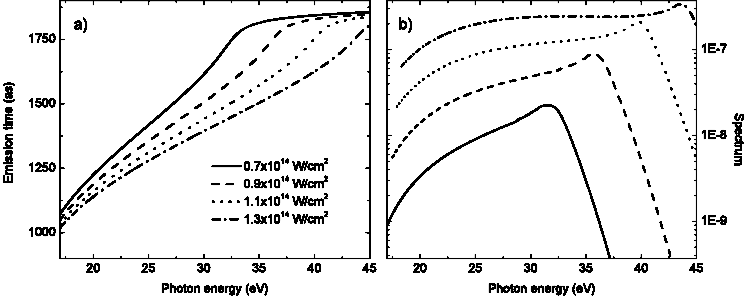
\includegraphics[width=0.8\columnwidth]{Figures/ThreeStep/gdd_argon.pdf}%
\caption{Temps d’émission (gauche) et intensité harmonique (droite) en fonction de l’énergie de photon harmonique et pour différentes intensités de génération. Calcul fait pour l’argon en ne considérant que la trajectoire courte de la GHOE. Tiré de \mycite{DivekiPhD2011}.}
\label{fig:diveki}
\end{figure}

Cette pente linéaire, couramment appelée \textit{atto-chirp}, est donc intrinsèque au mécanisme de génération lui-même \mycite{KazamiasPRA2004}. Elle peut être mesurée expérimentalement, par exemple par la technique RABBIT \mycite{DinuPRL2003,MairesseScience2003}, dont il sera question à la partie \ref{sec:omabbit}. Sa mesure permet également de la compenser, de sorte à comprimer les impulsions attosecondes générées.

\subsection{Phase spatiale des trajectoires quantiques}
\label{sec:phase_spatiale}
Nous avons jusqu'à présent considéré un unique atome émettant un rayonnement harmonique. En réalité, le faisceau de génération a une extension transverse bien plus large qu'un atome, le rayonnement émis est donc la somme cohérente de la contribution de chaque atome unique. Si le faisceau de génération a un profil d'intensité transverse gaussien, son intensité n'est pas uniforme. Nous allons voir que cela se traduit par une phase spatiale non homogène dans l'émission harmonique. On utilise les coordonnées cylindriques $(r,\theta,z)$. En un point $(r,\theta)$ dans le plan transverse, la phase du champ harmonique pour la trajectoire $j$ est donnée par :
\begin{equation}
\phi^j_q = \omega_q t_r - \int_{t_i}^{t_r}\left(\frac{({\bm{p}+\bm{A(t')}})^2}{2}+I_p\right)\rmd t',
\end{equation} 
où $t_i,\;t_r$ et $\bm{p}$ sont les solutions des équations de phase stationnaire. La phase dépend de l'intensité via le potentiel vecteur $\bm{A}(t)$. 

Sur la figure \ref{fig:varju}, tirée de \mycite{VarjuJMO2005}, est tracée $\phi^j_q$ en fonction de l'intensité $I$ pour l'harmonique 19 et pour les deux premières trajectoires quantiques. On observe une dépendance quasiment linéaire, de pente beaucoup plus forte pour la trajectoire longue. Pour les harmoniques loin de l'énergie de coupure, on approxime une dépendance linéaire :
\begin{equation}
\phi^j_q = - \alpha_q^j I,
\label{eq:alphaI}
\end{equation}
où $\alpha_q^j$ est le coefficient de proportionnalité exprimé en $\si{\radian\cm\squared\per\W}$. Cette phase est appelée \textit{phase atomique}. $\alpha_q^{\text{courte}}$ est de l'ordre de $\SI{-1}{\radian\cm\squared\per\W}$ tandis que $\alpha_q^{\text{longue}}\sim\SI{-25}{\radian\cm\squared\per\W}$. Sur le panneau de droite de la figure \ref{fig:varju} est tracé $\partial\phi^j_q/\partial I$ en fonction de l'ordre harmonique. $\alpha_q^{\text{courte}}$ est donc une fonction croissante de l'ordre harmonique, tandis que $\alpha_q^{\text{longue}}$ est décroissante. Dans la coupure, les deux trajectoires se confondent et convergent vers $\approx \SI{-12}{\radian\cm\squared\per\W}$\par
Si on considère maintenant la phase macroscopique du faisceau $\phi^j_q(r,\theta)$ pour une intensité gaussienne, on aura une courbure de phase : la dépendance en intensité du dipôle harmonique modifie la divergence de chaque harmonique. Pour les harmoniques les plus basses, les trajectoires longues auront une divergence bien plus grande que les courtes. Quand l'ordre harmonique augmente, la divergence des trajectoires courtes (resp. longues) augmente (resp. diminue) jusqu'à se confondre à la coupure. Cet effet est bien visible sur les spectres expérimentaux présentés plus loin (figure \ref{Fig:SpectrumGAr}). Il jouera également un rôle central dans la GHOE par un faisceau de Laguerre-Gauss (partie \ref{sec:pmodes}).

\begin{figure}[!ht]
\centering
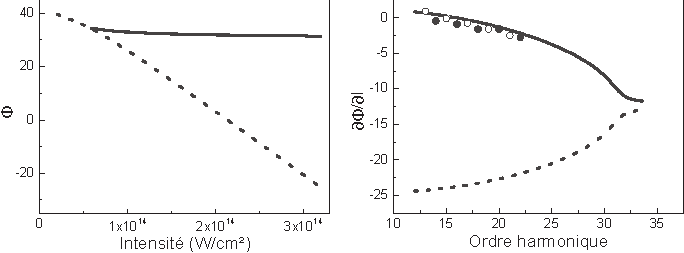
\includegraphics[width=1\columnwidth]{Figures/ThreeStep/alphaI_varju.pdf}%
\caption{Variation de la phase $\phi^j_q$ avec l'intensité (gauche). Le calcul est réalisé pour l'harmonique 19. Variation de $\partial\phi^j_q/\partial I$ avec l'ordre harmonique (droite), à une intensité de $\SI{1.5e15}{\W\per\cm\squared}$. Les lignes continues (resp. pointillées) correspondent aux trajectoires courtes (resp. longues).}
\label{fig:varju}
\end{figure}

\subsection{Accord de phase}
Ces considérations nous amènent à discuter d'un dernier point : l'accord de phase dans la GHOE. Nous avons déjà mentionné que le rayonnement était la somme cohérente de la contribution de chaque atome dans la zone d'interaction. Cette somme doit être réalisé selon la dimension transverse, $(r,\theta)$, et longitudinale, $z$. Si les différentes contributions ne sont pas en phase, des interférences destructives empêcheront l'émission macroscopique de rayonnement XUV. La compréhension de ce phénomène est essentielle pour expliquer les propriétés macroscopiques du rayonnement \mycite{SalieresPRL1995} et pour optimiser le rendement du processus \mycite{KazamiasPRL2003}.

Notons $\bm{k}_q$ le vecteur d'onde de l'harmonique d'ordre $q$ et $\bm{k}_1$ celui du faisceau gaussien de génération. \`A ces deux quantités s'ajoutent des termes de désaccord de phase dus à la phase atomique ainsi qu'à la dispersion électronique et ionique, que l'on note $\Delta \psi_q(r,\theta)$. La condition d'accord de phase pour l'harmonique $q$ s'écrit alors \mycite{BalcouPRA1997} :
\begin{equation}
\bm{k}_q(r,\theta,z) = q\bm{k}_1(r,\theta,z) + \Delta \psi_q(r,\theta,z)
\end{equation}
\mycite{BalcouPRA1997} évaluent le désaccord de phase $|\delta \bm{k}_q| = |\bm{k}_q-q\bm{k}_1 - \Delta \psi_q|$, en négligeant les effets de dispersion sur le laser. La figure \ref{fig:balcou} montre ce désaccord de phase pour les trajectoires courtes et longues. 

\begin{figure}[!ht]
\centering
\includegraphics[width=1\columnwidth]{Figures/ThreeStep/phasematching_balcou.pdf}%
\caption{Désaccord de phase pour les trajectoires longues (gauche) et courtes (droite). Les zones les plus claires indiquent un bon accord de phase. Les pointillés verticaux indiquent les positions des optima de génération d'harmonique. Les flèches représentent la direction d'émission du champ harmonique. Le calcul a été réalisé à une intensité de de \SI{6e14}{\W\per\cm\squared} dans le néon, pour l'harmonique 45. Le paramètre confocal est de 5 mm. Tiré de \mycite{BalcouPRA1997}.}
\label{fig:balcou}
\end{figure}

\'Etudions le cas de la trajectoire longue. On observe une structure particulière, en forme de "moustache de morse". On a deux zones notée B et D où le désaccord de phase est minimisé. La zone notée B est située sur l'axe optique mais est très fine, tandis que la zone D est assez étendue et est située en dehors de l'axe optique. De par le volume disponible, la génération d'harmonique proviendra principalement de la zone D. Les flèches indiquent une émission très divergente, ce qui est dû à l'effet de la phase atomique décrit plus haut. Notons également que la zone D se situe en amont de $z=0$, position du foyer du laser de génération. Pour la trajectoire courte (panneau de droite), le comportement est plus simple : on a un maximum du désaccord de phase vers $z\approx-0.5$ mm, qui diminue ensuite dans toutes les directions. Si on s'éloigne trop du foyer laser, l'intensité devient trop faible pour avoir une génération efficace. \mycite{BalcouPRA1997} montrent que l'optimum se situe à $z=3$ mm, où on a un désaccord faible sur un grand volume. 

En conclusion, nous avons mis en évidence deux familles de trajectoires électroniques, qui donnent lieu à deux composantes dans l'émission harmoniques de propriétés différentes. Finalement, nous avons vu que l'accord de phase permet de favoriser l'une ou l'autre : la trajectoire courte sera accordée lorsque le foyer optique se situe en amont du jet de gaz, tandis que la longue le sera lorsqu'il se situe en aval. Pour une description plus complète de la théorie de la GHOE, on se reportera à \mycite{ScrinziJPB2006} et à \mycite{SmirnovaIvanov2014}. Le modèle SFA présenté ici est la base des calculs numériques présentés plus loin (partie \ref{sec:sfa}), qui prendront en compte tous les effets de propagation et d'accord de phase dans le milieu. Dans la suite de cette partie, nous expliquons comment réaliser une expérience de GHOE dans le cas habituel d'un faisceau de génération gaussien.

\chapter{Aspects expérimentaux de la génération d'harmoniques d'ordre élevé}
\label{Sec:HHG_G}
\section{Système laser}
\label{sec:laser}
Toutes les expériences présentées dans ce chapitre et dans la partie \ref{PA:OAM_HHG} ont été réalisées sur le laser LUCA (Laser Ultra-Court Accordable) du LIDYL au CEA Saclay. Il s'agit d'un laser basé sur la technique "Chirped Pulse Amplification" utilisant le titane saphir comme milieu à gain. Partant d'un oscillateur femtoseconde oscillant autour de 800 nm, le faisceau est étalé temporellement avant d'être amplifié d'abord dans un amplificateur régénératif, puis dans un amplificateur multi-passages. Il est finalement recomprimé dans un compresseur à réseaux \mycite{StricklandOC1985}. La spécificité de ce système est l'insertion récente, juste avant la compression, d'un étage de filtrage modal \mycite{MahieuAPB2015}. Il s'agit d'une fibre creuse de 30 cm de long et $\SI{128}{\micro\metre}$ de diamètre dans laquelle le faisceau est injecté avant d'être collimaté de nouveau. Ceci a pour effet de sélectionner un mode de propagation très proche d'un mode gaussien pur. Finalement on obtient des impulsions dont l'intensité a une enveloppe temporelle gaussienne de largeur à mi-hauteur $\tau = 50$ fs et un profil spatial gaussien de largeur $w_0 = 15$ mm à $\frac{1}{e^2}$. La longueur d'onde utilisée est 792 nm, et l'énergie par impulsion est de 35 mJ pour un taux de répétition de 20 Hz. 

\section{Génération d'harmoniques d'ordre élevé}
Nous commençons par mettre en forme le faisceau laser : son diamètre est ajusté à l'aide d'un iris et son énergie est ajustée grâce à un atténuateur constitué d'une lame demi-onde et d'une paire de polariseur croisés. \`{A} la sortie de cet atténuateur, la polarisation du laser est verticale (S). Le faisceau est ensuite focalisé par une lentille dans un jet de gaz délivré par une vanne pulsée à la fréquence du laser par un système piezo-électrique (Attotech). L'utilisation d'une vanne pulsée permet de n'envoyer du gaz que lorsque le faisceau laser est présent, ce qui limite la pression résiduelle dans les chambres à vide. Ainsi, on peut atteindre une pression assez élevée ($\simeq$10 mbar) dans la région focale sans que l'émission harmonique ne soit réabsorbée par le gaz résiduel. Un autre paramètre important est le diamètre de l'orifice de la vanne (ici, 150 $\si{\micro\metre}$) : en choisissant un diamètre faible, on crée une extension supersonique du gaz ce qui garantit une longueur d'interaction avec le laser courte dans la direction longitudinale. On s'approche ainsi des conditions idéales d'un plan d'atomes, ce qui limite l'importance des effets d'accord de phase dans la GHOE. \par
Le choix du gaz dépend de l'expérience réalisée : on peut par exemple utiliser une molécule dont on étudie la réponse - c'est le principe de la spectroscopie harmonique. Dans notre cas le gaz n'est pas l'objet d'étude et on préférera utiliser un système simple, facile à se procurer, et ayant une grande section efficace. Le gaz le plus courant est l'Argon, qui est peu coûteux et génère de manière très efficace. Son potentiel d'ionisation est de 15.76 eV, ce qui donne une énergie de coupure assez faible et qui empêche de générer des ordres harmoniques très élevés. Dans les cas où on désire générer des ordres élevés et nombreux, on pourra utiliser d'autres gaz rares comme le Néon ($I_p$ = 21.6 eV), bien que la génération soit moins efficace.

Pour notre système, les paramètres nominaux sont :
\begin{itemize}
\item Le diamètre avant focalisation \O{} $\approx$ 10-15 mm,
\item L'énergie par impulsion de l'ordre de E = 1-3 mJ,
\item La lentille de longueur focale f = 1 m. \\
\end{itemize}
Pour connaître la valeur de l'intensité pic au foyer, le profil du faisceau après focalisation peut être calculé numériquement. Le champ avant la lentille est défini dans les coordonnées cylindriques $(R,\theta)$ par :
\begin{equation*}
E(R,\theta) = \sqrt{I_0} \exp{\left(-\frac{R^2}{w_0^2}\right)}\times\delta(\frac{\mbox{\O}}{2}-R),
\end{equation*}
où $w_0$ est la largeur du faisceau collimaté avant l'iris, \O{}  est le diamètre de l'iris, $\delta$ est la fonction de Heaviside, et $I_0 = \frac{2E\sqrt{\frac{4\log{2}}{\pi}}}{\tau\pi w_0^2}$.
La focalisation d'un faisceau par une lentille mince peut être calculée par une transformée de Fourier (voir \mycite{Goodman}, un des ouvrages de référence pour l'optique de Fourier, et \mycite{Tan} pour des exemples d'implémentations numériques). Ces calculs permettent d'étudier l'influence des différents paramètres. Par exemple, on peut faire varier le diamètre de l'iris : la Figure \ref{Fig:IrisScan} montre le profil du faisceau au foyer quand \O{} varie entre 5 et 25 mm. On voit alors que l'intensité pic au foyer part d'une valeur $<10^{13}$ et monte jusqu'à $\SI{10e14}{W/cm²}$. On se trouve donc parfaitement dans le régime d'intensité nécessaire à la génération d'harmonique : l'intensité est suffisante pour enclencher une ionisation tunnel mais reste assez faible pour ne pas ioniser et dépléter tout le milieu.

\begin{figure}[!ht]
\centering
\def\svgwidth{\columnwidth}
\import{Figures/Iris_Scan/}{Fig_IrisScan.pdf_tex}
\caption{\'{E}volution du foyer lorsqu'on varie la taille de l'iris. De gauche à droite : (1) profil transverse de l'intensité au foyer, (2) intensité pic, (3) taille du waist. Les paramètres sont les suivants : E = 1 mJ, $w_0$ = 15 mm, $\tau$ = 50 fs, $\lambda$ = 792 nm, f = 1 m et \O{} variant de 5 à 25 mm par pas de 1 mm. Le calcul est réalisé sur une grille de 1025x1025 points correspondant à une taille réelle de 5*\O{}.}
\label{Fig:IrisScan}
\end{figure}

Les harmoniques d'ordre élevé du laser infrarouge sont ainsi générées par le gaz injecté près du foyer de la lentille. Pour leur détection et caractérisation, nous avons utilisé d'une part un spectromètre électronique à temps de vol, d'autre part un spectromètre de photons. Le premier requiert un rayonnement focalisé alors que le second accepte en entrée un rayonnement divergent. Afin de pouvoir utiliser ces deux diagnostics successivement, avant d'entrer dans le spectromètre, le rayonnement XUV est ré-imagé par un dispositif composé de deux optiques (représentées plus bas sur la figure \ref{Fig:ExpG}) :
\begin{enumerate}
\item Un miroir torique en or de 50 cm de focale. Le miroir travaille à $11.5\degres$ d'incidence rasante ($78.5\degres$ par rapport à la normale au miroir), ce qui permet d'avoir une réflectivité importante et plate sur la gamme spectrale considérée (voir Figure \ref{Fig:TorR}).

\begin{figure}[!ht]
\centering
\def\svgwidth{0.6\columnwidth}
\import{Figures/Reflect_Torique/}{torR.pdf_tex}
\caption{Réflectivité calculée du miroir torique en or à un angle d'incidence de $11.5\degres$. (CXRO, \mycite{Henke1993}).}
\label{Fig:TorR}
\end{figure}
Le miroir torique est utilisé dans une configuration 2f-2f de sorte à garder un rapport\shorthandoff{:} 1:1 \shorthandon{:}entre le foyer de génération et le second foyer. \`{A} la position de ce second foyer nous pouvons placer le spectromètre à temps de vol, qui sert dans le cas d'une mesure RABBIT (voir la partie \ref{sec:omabbit}). Un autre avantage de cette imagerie est d'éloigner la zone de génération, où la pression est élevée, du spectromètre de photons, qui requiert un vide de l'ordre de $10^{-5}$ mbar pour que les détecteurs fonctionnent.\\

\item La deuxième optique est une lame de Si$\mbox{O}_{\mbox{2}}$, qui joue le rôle de filtre de l'infrarouge de génération. La lame de silice est traitée antireflet pour l'infrarouge grâce à un dépôt de multicouches. La dernière de ces couches est en silice, ce qui, combiné à une bonne qualité de surface permet de réfléchir efficacement le rayonnement harmonique. La Figure \ref{Fig:SilR}, tirée de \mycite{MairessePhD}, présente la réflectivité de la lame pour le rayonnement harmonique et infrarouge. La réflectivité dans l'extrême ultra violet (XUV) est donc supérieure à 50\% jusqu'à l'ordre $\approx 37$, tandis que moins de 10\% de l'infrarouge est réfléchi. Le filtrage de l'infrarouge de génération est souvent crucial : il constitue un bruit de mesure non négligeable, sans compter qu'il peut facilement endommager des optiques ou des détecteurs en aval s'il est focalisé.

\begin{figure}[!ht]
\centering
\def\svgwidth{\columnwidth}
\import{Figures/Reflect_Silice/}{silR.pdf_tex}
\caption{Réflectivité de la lame de silice. \`{A} gauche, transmission et réflectivité à 800 nm en fonction de l'angle d'incidence rasante. Les pointillés repèrent notre angle de $11.5\degres$. \`{A} droite, réflectivité XUV mesurée (cercles bleus) et donnée par le CXRO (ligne violette) (\mycite{Henke1993}). Figure adaptée de \mycite{MairessePhD}.}
\label{Fig:SilR}
\end{figure}
\end{enumerate}

Comme nous le verrons plus loin, pour l'étude des faisceaux de Laguerre-Gauss, il sera crucial d'imager le spectre harmonique, c'est-à-dire de séparer les différents ordres harmoniques et de mesurer leurs propriétés spatiales. C'est le rôle du spectromètre de photons. Environ 50 cm en aval du second foyer, les harmoniques sont dispersées par un réseau à pas variable cylindrique Hitachi 001-0437 (voir \mycite{KitaAO1983} pour des détails sur son fonctionnement). Comme pour les réseaux à pas fixe, l'angle de réflexion d'un rayonnement monochromatique de longueur d'onde $\lambda$ est donné par la formule :
\begin{equation*}
m\lambda=\frac{\sin{\alpha}+\sin{\beta}}{\sigma},
\end{equation*}
où $m$ est l'ordre de diffraction considéré (généralement 1), $\sigma$ le nombre de trait par mètre (1200 traits/mm dans notre cas), $\alpha$ et $\beta$ les angles d'incidence et de réflexion, définis par rapport à la normale au réseau (la documentation donne $\alpha = 87$\degres{} pour un fonctionnement optimal).\par
Le réseau de diffraction est cylindrique, le rendant focalisant uniquement dans la dimension horizontale. Un rayonnement gaussien de faible largeur spectrale $\Delta\lambda$ et de largeur spatiale $w(z)$ formera donc dans le plan focal du réseau une fine ligne verticale de largeur proportionnelle à $\Delta\lambda$ et de hauteur $w(z)$. On image ainsi à la fois les dimensions spectrale et spatiale, si on suppose la symétrie cylindrique. Ce spectre est imagé par des galettes de micro-canaux couplées à un écran de phosphore, lui-même observé par une caméra CCD Basler A102f. 

L'intégralité du dispositif expérimental est représenté sur la Figure \ref{Fig:ExpG}.

\vspace{\baselineskip}
\begin{figure}[!ht]
\centering
\def\svgwidth{\columnwidth}
\import{Figures/Setup_G/}{setupG_wbitmap.pdf_tex}
\caption{Dispositif expérimental de génération et détection d'harmoniques d'ordre élevé.}
\label{Fig:ExpG}
\end{figure}

Les figures \ref{Fig:SpectrumGAr} et \ref{Fig:SpectrumGNe} présentent des spectres obtenus avec ce dispositif en utilisant respectivement l'argon et le néon comme gaz de génération. On observe les ordres harmoniques allant de 13 à 29 dans l'argon, et de 13 à 57 dans le néon. Le potentiel d'ionisation du Néon, plus élevé que celui de l'argon, a permis d'utiliser une intensité plus importante sans ioniser complètement le milieu. Conformément à la loi de coupure on obtient dans ce cas un spectre plus étendu. Sur le spectre de l'argon, on observe clairement les deux premières trajectoires quantiques de la GHOE (voir partie \ref{sec:thTraj}) : une contribution sur l'axe correspond à la trajectoire courte et une plus divergente et moins intense correspond à la trajectoire longue. Dans le cas du néon, les conditions d'accord de phase utilisées favorisent la trajectoire courte. On remarque également que la divergence de la trajectoire courte (resp. longue) augmente (rep. diminue) avec l'ordre harmonique, jusqu'à ce que les deux trajectoires se confondent dans la coupure. Notons finalement la présence sur le spectre du néon de pics satellites autour des harmoniques les plus basses : il s'agit des harmoniques plus élevées diffractées au second ordre par le réseau.
\begin{figure}[!ht]
\centering
\def\svgwidth{\columnwidth}
\import{Figures/Spectrum_G/}{Spectrum_G_Ar.pdf_tex}
\caption{Spectre d'harmoniques d'ordre élevé générées dans l'argon à partir d'un mode laser gaussien.}
\label{Fig:SpectrumGAr}
\end{figure}
\begin{figure}[!ht]
\centering
\def\svgwidth{\columnwidth}
\import{Figures/Spectrum_G/}{Spectrum_G_Ne.pdf_tex}
\caption{Spectre d'harmoniques d'ordre élevé générées dans le néon à partir d'un mode laser gaussien.}
\label{Fig:SpectrumGNe}
\end{figure}

%\part{Le moment angulaire de la lumière}
\label{PA:LightAM}
\chapter{Le moment angulaire en physique classique}
\label{CH:ClassicAM}
Dans ce chapitre, nous nous attacherons d'abord à définir le moment angulaire (MA) classiquement, dans le cas d'un objet quelconque puis pour le champ électromagnétique, en utilisant l'optique maxwellienne. Nous étudierons ensuite l'équation d'onde et le moment angulaire de plusieurs de ses solutions, mettant en évidence deux types de MA de nature différente. Pour comprendre la natures de ces MA, nous étudierons le concept de moment angulaire en mécanique quantique, où on trouvera deux composantes du moment angulaire : le moment angulaire de spin (MAS) et le moment angulaire orbital (MAO). Le champ électromagnétique sera traité comme un système quantique, ce qui nous permettra de construire des champs pour lesquels le MAS et le MAO sont connus. En particulier, nous détaillerons la forme et les propriétés de ces champs. Nous terminerons par une discussion de l'échange de moment angulaire lors d'une interaction entre un laser et une molécule. Cette présentation nous fournira les outils utiles à l'analyse des expériences décrites dans le chapitre suivant.
\newpage
\section{Mécanique Lagrangienne}
\subsection{L'\'{e}quation de Lagrange}
\label{sec:lagrange}
En mécanique classique, l'évolution d'un objet est décrite par les lois de Newton. Pour un objet ponctuel, on a $\bm{F}=m\bm{\ddot{x}}$, où $\bm{F}$ est la somme des forces appliquées à cet objet, $m$ sa masse et $\bm{\ddot{x}}$ son accélération. Dans le cas d'objets plus complexes tels que ceux qui nous intéresserons dans ce chapitre, une description plus adaptée est celle développée par J.-L. Lagrange en 1764. Initialement utilisé pour l'étude de la libration de lune, ce formalisme a très largement dépassé son origine pour devenir une méthode générale de résolution de problèmes dynamiques. Le système y est décrit par un ensemble de \textit{coordonnées généralisées}, qui définissent l'espace des configuration. 

Par exemple, considérons un ensemble de particules soumises à un ensemble de forces conservatives décrites par un potentiel. De manière générale, on peut décrire l'état du système par un ensemble de coordonnées. Si on choisit les coordonnées cartésiennes dans un référentiel inertiel ${x_i}$, $i\in[1,\;N]$, l'équation de Newton s'écrit :
\begin{equation}
\label{eq:newton}
\forall i,\;m\ddot{x}_i = F_i.
\end{equation}
Remarquons que le terme de gauche est la dérivée de la quantité de mouvement $p_i=m\dot{x}_i=\partial T/\partial\dot{x}_i$, où $T$ est l'énergie cinétique. Le terme droite est la dérivée de l'énergie potentielle, $\partial U/\partial x_i$. Dans ces coordonnées, $T$ est indépendant de $x_i$ et $U$ est indépendant de $\dot{x}_i$. On définit alors le \textbf{Lagrangien} $L=T-U$, qui est une fonction des $x_i$ et des $\dot{x}_i$. On réécrit alors \ref{eq:newton} :
\begin{equation}
\label{eq:lag}
\frac{d}{dt}\frac{\partial L}{\partial \dot{x}_i}-\frac{\partial L}{\partial x_i}=0,
\end{equation}
qui est appelée \textbf{équation de Lagrange}. Montrons que cette équation est valable quelles que soient les coordonnées généralisée utilisée pour décrire le système. Supposons que l'espace des configurations soit décrit par ${q_j}$, $j\in[1,\;N]$, qui s'écrivent en fonction des coordonnées cartésiennes ${x_i}$ et du temps :
\begin{equation*}
\begin{split}
\forall j, q_j=q_j(x_1,\ldots,x_N,t)\text{ et inversement, }
\end{split}
\begin{split}
\forall i, x_i=x_i(q_1,\ldots,q_N,t).
\end{split}
\end{equation*}
Réécrivons l'équation de Lagrange \ref{eq:lag} en fonction des ${q_j}$. On a : 
\begin{equation}
\label{eq:lag1}
\frac{\partial L}{\partial \dot{x}_i} = \sum_j \frac{\partial L}{\partial q_j} \frac{\partial q_j}{\partial \dot{x}_i}+ \sum_j\frac{\partial L}{\partial \dot{q}_j}\frac{\partial \dot{q}_j}{\partial \dot{x}_i}.
\end{equation}
$q_j$ ne dépend que de $x_i$ et $t$, donc ${\partial q_j}/{\partial \dot{x}_i}=0$ et le premier terme s'annule. De plus,
\begin{equation}
\dot{q}_j = \sum_i \frac{\partial q_j}{\partial x_i}\dot{x}_i+\frac{\partial q_j}{\partial t}\text{,  donc  }
\frac{\partial \dot{q}_j}{\partial \dot{x}_i}=\frac{\partial q_j}{\partial x_i}.
\label{eq:lag3}
\end{equation}
\ref{eq:lag1} donne donc :
\begin{equation}
\label{eq:lag2}
\frac{\partial L}{\partial \dot{x}_i} = \sum_j\frac{\partial L}{\partial \dot{q}_j}\frac{\partial q_j}{\partial x_i}.
\end{equation}
L'équation de Lagrange en coordonnées cartésiennes comprend la dérivée temporelle de cette expression, qui s'écrit :
\begin{align*}
\frac{d}{dt}\frac{\partial L}{\partial \dot{x}_i} &= 
\sum_j\left(\frac{d}{dt}\frac{\partial L}{\partial \dot{q}_j}\right)\frac{\partial q_j}{\partial x_i}+
\sum_j\frac{\partial L}{\partial \dot{q}_j}\left(\frac{d}{dt}\frac{\partial q_j}{\partial x_i}\right) \\
&=\sum_j \left(\frac{d}{dt}\frac{\partial L}{\partial \dot{q}_j}\right)\frac{\partial q_j}{\partial x_i}+\sum_j\frac{\partial L}{\partial \dot{q}_j}\left(\sum_k \frac{\partial^2q_j}{\partial x_i \partial x_k}\dot{x}_k + \frac{\partial^2q_j}{\partial x_i \partial t}\right).
\end{align*}
Par ailleurs, le second terme de l'équation de Lagrange s'écrit :
\begin{align*}
\frac{\partial L}{\partial x_i}&= \sum_j \frac{\partial L}{\partial q_j} \frac{\partial q_j}{\partial x_i}+ \sum_j\frac{\partial L}{\partial \dot{q}_j}\frac{\partial \dot{q}_j}{\partial x_i} \\
&=\sum_j \frac{\partial L}{\partial q_j} \frac{\partial q_j}{\partial x_i}+ \sum_j\frac{\partial L}{\partial \dot{q}_j}\left(\sum_k \frac{\partial^2q_j}{\partial x_i \partial x_k}\dot{x}_k + \frac{\partial^2q_j}{\partial x_i \partial t}\right),
\end{align*}
où on a utilisé \ref{eq:lag3}. On connaît maintenant tous les termes de l'équation de Lagrange en fonction des ${q_j}$, et en les soustrayant un terme s'annule, ce qui donne :
\begin{equation*}
\sum_j\left(\frac{d}{dt}\frac{\partial L}{\partial \dot{q}_j}-\frac{\partial L}{\partial q_j}\right)\frac{\partial q_j}{\partial x_i}=0.
\end{equation*}
$\frac{\partial q_j}{\partial x_i}$ est non singulière puisque son inverse est $\frac{\partial x_i}{\partial q_j}$, on obtient donc l'équation de Lagrange en coordonnées généralisées : 
\begin{equation}
\label{eq:lagq}
\frac{d}{dt}\frac{\partial L}{\partial \dot{q}_i}-\frac{\partial L}{\partial q_i}=0.
\end{equation}
Nous avons donc démontré que l'équation de Lagrange est invariante par changement des coordonnées utilisées pour décrire le système, ce qui en fait une formulation très pratique. 

\subsection{Symétries du Lagrangien et lois de conservation}
\label{sec:symlagrange}
L'équation de Lagrange permet d'obtenir des résultats généraux assez directement, tels que des lois de conservation. Une coordonnée $q_k$ est dite \textit{ignorable} ou \textit{cyclique} si le Lagrangien $L$ ne dépend pas de $q_k$. L'équation de Lagrange donne alors :
\begin{equation*}
\frac{d}{dt}\frac{\partial L}{\partial \dot{q}_k} = \frac{\partial L}{\partial q_k} = 0.
\end{equation*}
On définit naturellement la grandeur 
\begin{equation*}
P_k\equiv\frac{\partial L}{\partial \dot{q}_k},
\end{equation*}
appelé \textit{moment généralisé conjugué} de $q_k$, et qui est une constante du mouvement. Nous allons utiliser ce point pour établir trois lois de conservation : l'énergie, la quantité de mouvement et le moment angulaire.

\subsubsection{\'{E}nergie et translation dans le temps}
La dérivée temporelle du Lagrangien s'écrit : 
\begin{align*}
\frac{dL}{dt}&=\sum_i\frac{\partial L}{\partial q_i}\frac{\partial q_i}{\partial t}+\sum_i\frac{\partial L}{\partial \dot{q}_i}\frac{\partial \dot{q}_i}{\partial t}+\frac{\partial L}{\partial t}\\
&= \sum_i\left(\frac{d}{dt}\frac{\partial L}{\partial \dot{q}_i}\right)\frac{\partial q_i}{\partial t}+\sum_i\frac{\partial L}{\partial \dot{q}_i}\frac{\partial \dot{q}_i}{\partial t}+\frac{\partial L}{\partial t}\\
&= \sum_i\frac{d}{dt}\left(\frac{\partial L}{\partial \dot{q}_i}\dot{q}_i\right)+\frac{\partial L}{\partial t}.
\end{align*}
Soit :
\begin{equation*}
\frac{d}{dt}\left(\sum_i\frac{\partial L}{\partial \dot{q}_i}\dot{q}_i-L\right)+\frac{\partial L}{\partial t}=0.
\end{equation*}
On définit alors la \textit{fonction énergie}\footnote{La fonction énergie semble avoir la même définition que l'Hamiltonien $H$ du système. Ils sont en effet égaux en valeur mais de nature différente : $h$ est une fonction des $N$ variables ${q_i}$, de leurs dérivées et éventuellement le temps, tandis que $H$ est une fonction de $2N$ variables ${q_i,p_i}$ et éventuellement du temps. Cette distinction est centrale pour la définition de la physique Hamiltonienne.} ou \textit{invariant de Jacobi} :
\begin{equation*}
h(q,\dot{q},t) = \sum_i\frac{\partial L}{\partial \dot{q}_i}\dot{q}_i-L,
\end{equation*}
on a donc 
\begin{equation*}
\frac{dh}{dt} = -\frac{\partial L}{\partial t}
\end{equation*}
On voit que si le Lagrangien ne dépend pas explicitement du temps, i.e. est invariant par translation temporelle, alors $h$ est conservé. Dans de nombreux cas, $h$ peut se réduire à l'énergie mécanique du système (voir p. 62 de \mycite{Goldstein2001}). Le résultat obtenu est alors la \textit{conservation de l'énergie mécanique}. 


\subsubsection{Quantité de mouvement et translation dans l'espace}
Considérons maintenant un système invariant par translation dans l'espace. C'est le cas d'une particule libre, ou encore de $N$ particules reliées par des interactions ne dépendant que de leur coordonnées relatives $\left|\bm{r}_i-\bm{r}_j\right|$. 
On note $\bm{r}_i(t)$ la trajectoire des particules et on considère une translation infinitésimale du système de coordonnées : $\bm{r}_i\rightarrow \bm{r}_i+\epsilon$. Le changement du Lagrangien vaut :
\begin{align*}
\delta L =\sum_i \epsilon\cdot\frac{\partial L}{\partial \bm{r}_i}= \epsilon\cdot\frac{d}{dt}\sum_i \frac{\partial L}{\partial {\dot{\bm{r}}}_i}
\end{align*}
Si le système est invariant par rapport à la translation, alors $\delta L=0$ et la quantité de mouvement totale
\begin{equation*}
\bm{P}\equiv\sum_i\frac{\partial L}{\partial \dot{\bm{r}}_i}
\end{equation*}
est conservée. Si l'invariance n'est vraie que dans une direction, alors seulement la composante de $\bm{P}$ dans cette direction sera conservée.


\subsubsection{Moment angulaire et rotation}
Enfin, considérons un système invariant par rotation autour d'un axe $\bm{u}$. Prenons une rotation infinitésimale d'angle $\delta\theta$ et notons $\delta\bm{\theta}=\bm{u}\delta\theta$. Si on choisit l'origine du repère sur l'axe de rotation, le changement pour chaque vecteur de coordonnées est $\delta\bm{r}_i(t) = \delta\bm{\theta}\times\bm{r}_i(t)$. De même, $\delta\bm{\dot{r}}_i(t) = \delta\bm{\theta}\times\bm{\dot{r}}_i(t)$. Le changement du Lagrangien est :
\begin{align*}
\delta L &=\sum_i \left(\delta\bm{\theta}\times\bm{r}_i(t)\right)\cdot\frac{\partial L}{\partial \bm{r}_i}+\sum_i \left(\delta\bm{\theta}\times\bm{\dot{r}}_i(t)\right)\cdot\frac{\partial L}{\partial \bm{\dot{r}}_i}\\
&=\delta\bm{\theta}\cdot\sum_i\left(\bm{r}_i(t)\times\frac{d}{dt}\frac{\partial L}{\partial {\dot{\bm{r}}}_i}
+\bm{\dot{r}}_i(t)\times\frac{\partial L}{\partial \bm{\dot{r}}_i}\right)\\
&=\delta\bm{\theta}\cdot\sum_i\frac{d}{dt}\left(\sum_i \bm{r}_i(t)\times\frac{\partial L}{\partial \bm{\dot{r}}_i}\right)
\end{align*}
où on a permuté circulairement les produits mixtes et utilisé l'équation de Lagrange. Si le Lagrangien est invariant par rotation, alors $\delta L = 0$ et on note $\bm{J}$ la quantité conservée suivante :
\begin{equation}
\bm{J}\equiv\sum_i \bm{r}_i(t)\times\frac{\partial L}{\partial \bm{\dot{r}}_i}=\sum_i \bm{r}_i\times\bm{p}_i.
\label{eq:defJ}
\end{equation}
$J$ est le \textit{moment angulaire} du système. Il est clair que sa valeur dépend du choix du centre du système de coordonnées. Si on applique $\bm{r}_i\rightarrow \bm{r}_i+\bm{a}$, alors $\bm{J}\rightarrow \bm{J}+\bm{a}\times\bm{P}$. Notons que dans le référentiel du centre de masse (c.d.m.), $\bm{P}=0$. $\bm{J}$ est alors indépendant du choix de l'origine des coordonnées. Pour des raisons qui paraîtront claires plus tard, notons $\bm{S}$ la valeur de $\bm{J}$ dans le référentiel du c.d.m. Dans un référentiel où le c.d.m se déplace à une vitesse uniforme $\bm{V}$, 
\begin{align*}
\bm{J}&=\sum_i \left(\bm{r}_i+\bm{V}t\right)\times\left(\bm{p}_i+m_i\bm{V}\right)\\
&= \sum_i\bm{r}_i\times\bm{p}_i+\bm{V}t\times\bm{P}+\sum_i m_i\bm{r}_i\times\bm{V} \\
&= \bm{S} + M \bm{R}_{cdm}\times\bm{V} = \bm{S} + \bm{R}_{cdm}\times\bm{P}.
\end{align*}
où $M=\sum_i m_i$ est la masse totale du système et $\bm{R}_{cdm}$ la position du centre de masse. On décompose donc le moment angulaire total en deux parties : $\bm{S}$, qui est indépendante du choix du repère, et $\bm{R}_{cdm}\times\bm{P}$.

\section{Les propriétés mécaniques de la lumière}
Comme nous l'avons fait pour la matière, nous établissons ici les expressions de l'énergie, de la quantité de mouvement et du moment angulaire associé à un rayonnement électromagnétique.

\subsection{L'énergie du champ électromagnétique} 
Définir l'énergie du champ électromagnétique a donné lieu à de vifs débats à la fin du XIXème siècle, liés aux discussions sur la propagation d'une onde dans le vide. Dans une série de travaux pionniers, John H. Poynting a largement clarifié les dicussions au sujet de l'énergie des ondes électromagnétiques, la pression de radiation, et même le moment angulaire de la lumière. Poynting faisait partie d'un groupe de physiciens mené par Heaviside, Fitzgerald, Lodge et Hertz qui travaillèrent à développer la théorie de Maxwell après sa mort en 1873. Nous reprenons ici la démarche de son article de 1884 \mycite{Poynting1884}, qui amène à une expression de la densité d'énergie et du flux d'énergie d'un champ électromagnétique.

Considérons une distribution de charges et de courants contenus dans un volume $V$. En un court temps $\rmd t$, une charge bougera de $\bm{v}\rmd t$. En utilisant l'expression de la force de Lorentz, le travail effectué sur la charge sera
\begin{equation*}
\rmd W = \bm{F}\cdot\bm{\rmd l} = q(\bm{E}+\bm{v}\times\bm{B})\cdot\bm{v}\rmd t = q\bm{E}\cdot \bm{v} \rmd t,
\end{equation*}
où l'on retrouve que la force magnétique ne fournit pas de travail. Notons ensuite $\rho$ la densité de charge dans le volume ($q = \rho \rmd V$) et $\bm{J} =\rho \bm{v}$ la densité de courant. En intégrant sur le volume V, on obtient
\begin{equation*}
\frac{\rmd W}{\rmd t} = \int_V \bm{E} \cdot \bm{J} \rmd V.
\end{equation*}
$\rmd W/\rmd t$ est le taux auquel le travail est fourni, c'est-à-dire la puissance délivrée au système. $\bm{E} \cdot \bm{J}$ est donc la puissance délivrée par unité de volume, que l'on peut exprimer en utilisant l'équation de Maxwell-Ampère :
\begin{align*}
\bm{E} \cdot \bm{J} &= \frac{1}{\mu_0}\bm{E} \cdot (\bm{\nabla} \times \bm{B})-\epsilon_0\bm{E}\cdot\frac{\partial\bm{E}}{\partial t}\\
&= \frac{1}{\mu_0}\bigl[\bm{B} \cdot (\bm{\nabla} \times \bm{E})-\bm{\nabla} \cdot (\bm{E} \times \bm{B})\bigr]-\epsilon_0\bm{E}\cdot\frac{\partial\bm{E}}{\partial t}\\
&= \frac{1}{\mu_0}\bigl[-\bm{B} \cdot \frac{\partial\bm{B}}{\partial t}-\bm{\nabla} \cdot (\bm{E} \times \bm{B})\bigr]-\epsilon_0\bm{E}\cdot\frac{\partial\bm{E}}{\partial t}
\end{align*}
On note que $\bm{B} \cdot \frac{\partial\bm{B}}{\partial t} = \frac{1}{2}\frac{\partial\bm{B^2}}{\partial t}$ et $\bm{E} \cdot \frac{\partial\bm{E}}{\partial t} = \frac{1}{2}\frac{\partial\bm{E^2}}{\partial t}$ et on obtient
\begin{equation*}
\bm{E} \cdot \bm{J} = -\frac{1}{2}\frac{\partial}{\partial t}\biggl(\epsilon_0\bm{E^2}+\frac{1}{\mu_0}\bm{B^2}\biggl)-\frac{1}{\mu_0}\bm{\nabla} \cdot (\bm{E} \times \bm{B})
\end{equation*}
En intégrant cette équation sur le volume $V$ et en utilisant le théorème d'Ostrogradski sur le dernier terme, elle se réécrit
\begin{equation}
\frac{\partial}{\partial t}\int_V\frac{1}{2}\biggl(\epsilon_0\bm{E^2}+\frac{1}{\mu_0}\bm{B^2}\biggl)\rmd V+\frac{1}{\mu_0} \oint_S(\bm{E} \times \bm{B})\cdot\bm{\rmd S}=-\frac{\rmd W}{\rmd t},
\label{eq:continuityE}
\end{equation}
On identifie deux quantités : 
\begin{equation}
U=\frac{1}{2}\biggl(\epsilon_0\bm{E^2}+\frac{1}{\mu_0}\bm{B^2}\biggr) \mbox{   et   } \bm{\Pi} = \frac{1}{\mu_0}\bm{E}\times\bm{B}
\label{Def.Poynting}
\end{equation}
$U$ est la \textbf{densité d'énergie} (énergie par unité de volume) et $\bm{\Pi}$ est la \textbf{densité de flux d'énergie} (énergie par unité de surface par unité de temps). L'équation \ref{eq:continuityE} est donc une équation de conservation de l'énergie qui se comprend ainsi :

Le taux de variation de l'énergie électromagnétique dans V + L'énergie qui sort du volume en traversant la surface S = L'opposé du travail total effectué par le champ sur les sources dans V.

$\bm{\Pi}$ est connu sous le nom de \textbf{vecteur de Poynting}. De manière intéressante, si on considère une onde plane se propageant selon un vecteur d'onde $\bm{k}$, on voit que $\bm{\Pi}$ est parallèle à $\bm{k}$. Ce n'est pas le cas de manière générale : $\bm{k}$ pointe dans la direction de la vitesse de phase alors que $\bm{\Pi}$ pointe dans celle de la vitesse de groupe. De nombreux exemples montrent que ces quantités sont distinctes, tel que la biréfringence ou le phare attoseconde (\mycite{VincentiPRL2012}). 

\subsection{La quantité de mouvement de la lumière}
Nous avons démontré la conservation de l'énergie du système combiné du champ et des particules. De la même façon, la quantité de mouvement de ce système doit être conservée. On note $\bm{P}_{part}$ la somme des quantités de mouvement des particules dans le volume V. La seconde loi de Newton donne :
\begin{equation*}
\frac{d\bm{P}_{part}}{dt}=\int_V \rho \bm{E} + \bm{J}\times\bm{B}\;\rmd V.
\end{equation*} 
On utilise l'équation de Maxwell-Gauss et de Maxwell-Ampère pour écrire :
\begin{align*}
\rho \bm{E} + \bm{J}\times\bm{B} &= \frac{1}{\mu_0} \bm{E}\cdot(\bm{\nabla}\cdot\bm{E})+\epsilon_0 \bm{B}\times\frac{\partial \bm{E}}{\partial t}-\frac{1}{\mu_0}\bm{B}\times(\bm{\nabla}\times\bm{B})\\
&= \frac{1}{\mu_0} \bm{E}\cdot(\bm{\nabla}\cdot\bm{E})+\epsilon_0 
\left(-\frac{\partial}{\partial t}(\bm{E}\times\bm{B})+\bm{E}\times\frac{\partial \bm{B}}{\partial t}\right)
-\frac{1}{\mu_0}\bm{B}\times(\bm{\nabla}\times\bm{B})\\
&= \frac{1}{\mu_0} \bm{E}\cdot(\bm{\nabla}\cdot\bm{E})+\epsilon_0\left(-\frac{\partial}{\partial t}(\bm{E}\times\bm{B})-\bm{E}\times(\bm{\nabla}\times\bm{E})\right)
-\frac{1}{\mu_0}\bm{B}\times(\bm{\nabla}\times\bm{B}).
\end{align*} 
Finalement,
\begin{equation*}
\frac{d\bm{P}_{part}}{dt}+\epsilon_0\frac{d}{dt}\int_V (\bm{E}\times\bm{B})\; \rmd V=\int_V \left[\frac{1}{\mu_0} \bm{E}\cdot(\bm{\nabla}\cdot\bm{E})-\epsilon_0\bm{E}\times(\bm{\nabla}\times\bm{E})
-\frac{1}{\mu_0}\bm{B}\times(\bm{\nabla}\times\bm{B})\right]\rmd V.
\end{equation*} 

Comme démontré dans la section 6.9 de \mycite{Jackson1999}, le terme de droite est le flux du quantité de mouvement vers l'extérieur du volume V à travers la surface S. On identifie donc finalement la quantité de mouvement totale du champ électromagnétique :
\begin{align}
\bm{P}_{champ} &= \epsilon_0\frac{d}{dt}\int_V (\bm{E}\times\bm{B})\; \rmd V \nonumber\\
&= \frac{\bm{\Pi}}{c^2} \mbox{, où $\bm{\Pi}$ est donné par \ref{Def.Poynting}.}
\label{eq:defP}
\end{align}

C'est l'essence de la démarche utilisée par Henri Poincaré en 1900 \mycite{poincare1900}, où il discute de la \textit{``quantité de mouvement de [...] notre fluide fictif''}. Dans ce même article, Poincaré parle de la force exercée par la lumière sur la matière, notion déjà présente chez Maxwell et même chez Kepler appelée \textit{pression électromagnétique}. On l'appelle aujourd'hui plus couramment \textit{pression de radiation}. Poynting développa considérablement ce concept par la suite \mycite{poynting1903}, et nota que malgré sa faible valeur comparée à la force de gravitation, elle pourrait avoir d'importantes conséquences en astronomie. \`{A} raison : par exemple, si la pression de radiation n'avait pas été prise en compte lors du programme Viking, les deux sondes envoyées sur Mars auraient raté l'orbite de la planète d'environ 15000 kilomètres \mycite{Hecht2001}.

\subsection{Le moment angulaire de la lumière}
Poynting, en plus de ces contributions majeures, a été le premier à envisager l'existence du moment \textit{angulaire} de la lumière. Il fit l'analogie entre une onde électromagnétique polarisée circulairement et une onde élastique de torsion, suggérant que la lumière possède un moment angulaire et peut fournir un couple à la matière \mycite{PoyntingPRSL1909}. Il propose à la fin de son article un dispositif expérimental constitué d'une série de lames quart d'ondes, permettant de démultiplier cet effet jusqu'à le rendre mesurable. Il conclut toutefois avec pessimisme que \textit{``even with such multiplications, my present experience of light forces does not give me much hope that the effect could be detected, if it has the value suggested by the mechanical model''}.

Il aurait donc probablement été heureux d'apprendre qu'en 1936, R. A. Beth observa cet effet avec un schéma légèrement modifié \mycite{BethPR1936}, confirmant ainsi l'existence du moment angulaire de la lumière. \mycite{DelannoyAPL2005} réalisèrent une expérience similaire en utilisant de la soie d'araignée.\par
L'expression de la densité de moment angulaire du champ est directement obtenue en utilisant la définition \ref{eq:defJ} et l'expression \ref{eq:defP}:
\begin{equation}
\bm{J}(\bm{r})=\bm{r}\times\bm{\bm{P}_{champ}}=\frac{\bm{r}\times\bm{\Pi}}{c^2} = \epsilon_0\bm{r}\times(\bm{E}\times\bm{B})
\label{Eq.DefJEM}
\end{equation}

C'est l'expression classique du moment angulaire du champ électromagnétique, la quantité qui nous intéressera pendant la majorité de cette thèse. Nous allons maintenant étudier le moment angulaire de différentes solutions de l'équation d'onde.

\chapter{L'équation d'onde et les modes du champ}
\label{ch:modes}
\section{Ondes planes et polarisation}
\subsection{L'équation d'Helmholtz}
Par simplicité, nous ne considérerons pas la présence de densités de charges ou de courant. Dans ce cas, les équations de Maxwell donnent les équations d'onde :
\begin{align*}
&\nabla^2\bm{E}-\frac{1}{c^2}\frac{\partial^2}{\partial t^2}\bm{E}=0,
&\nabla^2\bm{B}-\frac{1}{c^2}\frac{\partial^2}{\partial t^2}\bm{B}=0.
\end{align*}
On considère maintenant des faisceaux monochromatiques de fréquence angulaire $\omega$. On introduit la notation complexe :
\begin{equation*}
\begin{split}
\bm{E}=\text{Re}[\bm{\mathcal{E}}\exp{(-\rmi\omega t)}]
\end{split}
\quad\text{et}\quad
\begin{split}
\bm{B}=\text{Re}[\bm{\mathcal{B}}\exp{(-\rmi\omega t)}],
\end{split}
\end{equation*}
qui permet d'obtenir l'équation d'Helmhotz :
\begin{align}
&\nabla^2\bm{\mathcal{E}}+k^2\bm{\mathcal{E}}=0,\nonumber\\
&\nabla^2\bm{\mathcal{B}}+k^2\bm{\mathcal{B}}=0,
\label{eq:helmhotz}
\end{align}
où $k=\omega/c$ est le nombre d'onde, norme du vecteur d'onde $\bm{k}$. On considère alors l'ansatz $\bm{\mathcal{E}}=\bm{\mathcal{E_0}}\rme^{\pm\rmi\bm{k}\cdot\bm{r}} = \bm{\mathcal{E_0}}\rme^{\pm\rmi(k_x x + k_y y + k_z z)}$. En l'insérant dans \ref{eq:helmhotz}, on obtient 
\begin{equation*}
k_x^2+k_y^2+k_z^2=\frac{\omega^2}{\rmc^2}
\end{equation*}
On suppose $k_x$, $k_y$, $k_z$ réels et on obtient 
\begin{equation*}
\bm{E}=\text{Re}[\mathcal{E_0}\exp{(\pm\rmi\bm{k}\cdot\bm{r}-\rmi\omega t)}],
\end{equation*}
qui sont appelées les ondes planes. Les solutions avec un signe $+$ (resp. $-$) se propagent dans la direction de (resp. inversement à) $\bm{k}$. Pour que ces solutions vérifient les équations de Maxwell, il reste à vérifier qu'elles sont de divergence nulle : $\bm{\nabla}\cdot\bm{E} = 0$. Par conséquent, $\bm{k}\cdot\bm{\mathcal{E_0}}= 0$ : le champ électrique est nécessairement perpendiculaire à $\bm{k}$, on parle d'onde transverse électrique. La direction du champ $\bm{B}$ est donnée par l'équation de Maxwell-Faraday : en notation complexe, $\bm{\nabla}\times\bm{\mathcal{E}}=-\rmi\omega\bm{\mathcal{B}}$. Ainsi, $\bm{B}$ est perpendiculaire à $\bm{E}$ et $\bm{k}$.

\subsection{La polarisation des ondes planes}
On choisit un repère cartésien tel que $\bm{k}=\bm{e_z}$. Un champ électrique transverse s'écrit :
\begin{equation*}
\bm{E}=\begin{pmatrix}
E_{0x}\cos{(\omega t-kz)}\\
E_{0y}\cos{(\omega t-kz-\phi)}\\
0
\end{pmatrix}
\end{equation*}
Le champ électrique décrit donc une ellipse dans le plan transverse. S'il la parcourt dans le sens trigonométrique autour de $\bm{k}$, on dit que la polarisation est elliptique gauche (PEG). Inversement, dans le sens des aiguille d'une montre la polarisation est elliptique droite (PED). On peut se placer dans le repère des axes de l'ellipse de sorte à ce que le champ s'écrive :
\begin{equation*}
\bm{E}=\begin{pmatrix}
E_{0x}\cos{(\omega t-kz)}\\
\pm E_{0y}\sin{(\omega t-kz)}\\
0
\end{pmatrix}
\end{equation*}
Le signe $+$ représente une PEG et $-$ une PED. Dans le cas particulier où $E_{0x}=E_{0y}$, l'ellipse devient un cercle et on dit que la polarisation est circulaire gauche (PCG) ou droite (PCD). Enfin, notons que la phase $\phi$ peut être nulle. Dans ce cas, la polarisation est rectiligne. Cette polarisation peut être construite en effectuant la somme d'une PEG et d'une PED. Inversement, une onde polarisée elliptiquement peut être vue comme la superposition de deux polarisations rectilignes.

\subsection{Moment angulaire d'une onde plane circulaire}
\label{sec:ma_circ}
Intéressons nous maintenant au moment angulaire porté par ces ondes planes. L'équation \ref{eq:defJ} donne son moment angulaire selon l'axe de propagation: 
\begin{align*}
\bm{J_z}&=(\bm{r}\times\bm{\Pi})\cdot\bm{e_z}\\
&=\frac{1}{\mu_0}(\bm{r}\times[\bm{E}\times\bm{B}])\cdot\bm{e_z}
\end{align*}
Il est clair que pour une onde plane $\bm{J_z}$ s'annule. Ceci contredit ce qui est observé dans l'expérience de Beth \mycite{BethPR1936} déjà mentionnée. En fait, ce cas est singulier : $\Pi_x$ et $\Pi_y $ sont nuls alors que l'extension transverse de l'onde est infinie. On est donc confrontés à une indétermination du type $0\times \infty$. 
Ce problème peut être résolu en restreignant le problème à un volume $V$ où l'on prend en compte rigoureusement les effets de bords, puis en faisant tendre les dimensions du volume vers l'infini : voir \mycite{StewartEJP2005}. Une autre approche intéressante est celle de \mycite{MansuripurOE2005}, qui considère 4 ondes planes se propageant avec un angle $\theta$ par rapport à $z$ dans chacun des quadrants de $(x,y)$. Chacune de ces ondes ayant un vecteur d'onde formant un angle avec $z$, $\bm{J_z}$ est non nul. Quand on somme le moment angulaire de ces 4 ondes, si $\theta$ est assez petit on obtient une quantité ne dépendant pas de $\theta$. Il reste ensuite à faire tendre $\theta$ vers 0 pour retrouver l'onde plane comme cas limite, avec un moment angulaire non nul.

Remarquons pour terminer que dans l'expérience de Beth, la lumière transmet du moment angulaire à un objet qui se met à tourner \textit{sur lui-même}, et pas par rapport au centre du faisceau. Ceci est cohérent avec la structure d'une onde plane : dans le plan transverse, son profil ne dépend pas du tout des coordonnées $(x,y)$. C'est bien sa polarisation, c'est-à-dire sa structure vectorielle intrinsèque, qui lui donne du moment angulaire. 

\section{L'approximation paraxiale}
En optique géométrique, un rayon est appelé \textit{paraxial} son inclinaison par rapport à l'axe optique est faible. En optique ondulatoire paraxiale, le spectre angulaire d'une onde doit être composé d'ondes planes paraxiales par rapport à la direction de propagation de l'onde. Cette condition est vérifiée dans la plupart des expériences de GHOE. Nous allons voir qu'elle permet de simplifier l'équation d'Helmholtz et d'en trouver des solutions.\par
On commence par transformer l'équation d'Helmholtz vectorielle en équation scalaire. Pour ce faire, on considère une onde de polarisation transverse à l'axe optique. On écrit alors:
\begin{equation}
\bm{\mathcal{V}}=\bm{t}\xi(\bm{r},z),
\label{eq:parax1}
\end{equation}
où $\bm{\mathcal{V}}$ est une grandeur vectorielle telle que le champ électrique, le champ magnétique ou le vecteur potentiel, $\bm{t}$ le vecteur de polarisation transverse unitaire et $\xi$ une grandeur scalaire fonction des deux coordonnées de l'espace transverse. En injectant \ref{eq:parax1} dans l'équation de Helmholtz, on obtient :
\begin{equation}
\nabla^2{\xi}+k^2{\xi}=0.
\label{eq:parax2}
\end{equation}
Pour une onde paraxiale, le vecteur d'onde $\bm{k}$ est principalement dirigé sur l'axe optique $\bm{e_z}$ :
\begin{equation*}
k_z = \sqrt{k^2-\kappa^2}\approx k-\frac{\kappa^2}{2k}.
\label{eq:parax3}
\end{equation*}
On choisit l'ansatz suivant :
\begin{equation}
\xi(\bm{r})=u(\bm{r},z)\exp{(\rmi k z)}.
\label{eq:parax4}
\end{equation}
$u(\bm{r},z)$ est une fonction d'amplitude. Elle peut varier avec la distance $z$, par diffraction ou effets de propagation, mais ces variations resteront faibles comparées à celles de $\exp{(\rmi k z)}$. On injecte \ref{eq:parax4} dans l'équation \ref{eq:parax2} pour obtenir :
\begin{equation}
\nabla_t^2 u+\frac{\partial^2}{\partial z^2} u + 2\rmi k \frac{\partial}{\partial z} u =0.
\label{eq:parax5}
\end{equation}
L'approximation paraxiale consiste à négliger $\frac{\partial^2}{\partial z^2} u$ par rapport aux autres termes de \ref{eq:parax5}, puisque $u$ varie lentement avec $z$. Comparons les différents termes :
\begin{equation}
\left|\frac{\partial^2}{\partial z^2} u\right|\ll k\left| \frac{\partial}{\partial z} u\right|
\label{eq:para6}
\end{equation}
Cette inégalité est vérifiée si le profil varie lentement avec $z$. En effet, la dérivée seconde de $u$ sera plus faible que sa dérivée première multipliée par le nombre d'onde.

\begin{equation}
\left|\frac{\partial^2}{\partial z^2} u\right|\ll\left|\nabla_t^2 u \right|
\label{eq:para7}
\end{equation}
Cette condition est problématique si on l'applique à l'équation d'Helmholtz pour le champ électrique. Un champ électrique dans le vide a une divergence nulle, ce qui implique que sa divergence dans la direction transverse est nulle : $\nabla_{\bm{t}} E=0$. Le Lapacien transverse est alors également nul, ce qui contredit l'inégalité \ref{eq:para7}. \mycite{DavisPRA1979} montre que ce problème peut être contourné en considérant à la place le potentiel vecteur $\bm{A}$ dans la jauge de Lorentz. Il est défini par :
\begin{equation}
\bm{B} = \bm{\nabla}\times\bm{A},
\label{eq:para8}
\end{equation}
ce qui avec l'équation de Maxwell-Faraday permet d'écrire : 
\begin{equation}
\bm{\nabla}\left(\bm{E}+\frac{\partial}{\partial t}\bm{A}\right) = 0.
\label{eq:para9}
\end{equation}
Il existe donc un potentiel scalaire $\Phi$ défini par :
\begin{equation}
\nabla\Phi=-\left(\bm{E}+\frac{\partial}{\partial t}\bm{A}\right).
\label{eq:para10}
\end{equation}
Les potentiels $\Phi$ et $\bm{A}$ ne sont pas définis de manière unique. Pour les fixer, on utilise une condition de jauge. La jauge de Lorentz est donné par :
\begin{equation}
\bm{\nabla}\cdot\bm{A}+\frac{1}{\rmc^2}\frac{\partial}{\partial t}\Phi=0.
\label{eq:para11}
\end{equation}
Avec cette condition et les équations de Maxwell, on obtient une équation d'Helmholtz pour le potentiel vecteur :
\begin{equation*}
\nabla^2\bm{A}+k^2\bm{A}=0,
\label{eq:para12}
\end{equation*}
où on a utilisé l'ansatz $\bm{A}=\text{Re}[\bm{\mathcal{A}}\exp{(-\rmi\omega t)}]$. L'inégalité \ref{eq:para7} est alors vérifiée avec $\bm{\mathcal{V}} = \bm{A}=\bm{t}\xi(\bm{r},z)=\bm{t}u(\bm{r},z)\exp{(\rmi k z)}$. On peut donc négliger $\frac{\partial^2}{\partial z^2} u$ et on obtient l'équation d'onde paraxiale :
\begin{equation}
\nabla_t^2 u+2\rmi k\frac{\partial}{\partial z}{u}=0.
\label{eq:para13}
\end{equation}
Une fois $\bm{A}$ obtenu, on peut retrouver les champs électrique et magnétique. Avec les notations complexes $\bm{E}=\text{Re}[\bm{\mathcal{E}}\exp{(-\rmi\omega t)}]$, $\bm{B}=\text{Re}[\bm{\mathcal{B}}\exp{(-\rmi\omega t)}]$ et $\Phi=\text{Re}[\phi\exp{(-\rmi\omega t)}]$, \ref{eq:para10} se réécrit :
\begin{align}
\bm{\mathcal{E}}&=-\nabla\phi +\rmi\omega\bm{\mathcal{A}}\\
&=-\bm{\nabla}\left(-\frac{\rmc^2\bm{\nabla}\cdot\bm{\mathcal{A}}}{\rmi \omega}\right)+\rmi\omega\bm{\mathcal{A}}\\
&=\rmi\omega\left(\bm{\mathcal{A}}+\frac{\bm{\nabla}(\bm{\nabla}\cdot\bm{\mathcal{A}})}{k^2}\right),
\label{eq:para14}
\end{align}
et 
\begin{equation}
\bm{\mathcal{B}} = \bm{\nabla}\times\bm{\mathcal{A}}.
\label{eq:para15}
\end{equation}

\section{Les modes de Hermite-Gauss et de Laguerre-Gauss}
\subsection{Modes de Hermite-Gauss}
Une solution de l'équation d'onde paraxiale \ref{eq:para13} couramment employé est la famille des modes de Hermite-Gauss (HG). On se place en coordonnées cartésiennes et comme expliqué plus haut, on écrit le vecteur potentiel :
\begin{equation*}
\bm{A}=\bm{e_x}u(x,y,z)\exp{(\rmi k z)},
\end{equation*}
où on a choisit la polarisation transverse $\bm{t}$ selon $\bm{e_x}$. Les modes de HG sont obtenus en séparant les variables transverses :
\begin{equation*}
u^{HG}_{nm}(x,y,z)=u^{HG}_{n}(x,z)u^{HG}_{m}(y,z),
\end{equation*}
où $n$ et $m$ sont les indices du mode dans chacune des directions transverses. $u^{HG}_{n}$ et $u^{HG}_{m}$ obéissent chacun à l'équation d'onde paraxiale à une dimension ; par exemple selon $x$ on a :
\begin{equation*}
\left(\nabla_t^2 +2\rmi k\frac{\partial}{\partial z}\right)u^{HG}_{n}(x,z)=0.
\end{equation*}
On vérifie que le champ suivant est une solution normalisée ce cette équation :
\begin{align}
u^{HG}_{n}(x,z)&=\frac{C_n^{HG}}{\sqrt{w(z)}}\exp{\left[\rmi k \frac{x^2 z}{2(z_R^2 + z^2)}\right]}\exp{\left(-\frac{x^2}{w^2(z)}\right)}\\
&\times \exp{\left[-\rmi\left(n+\frac{1}{2}\right)\chi(z)\right]}H_n\left(\frac{\sqrt{2}x}{w(z)}\right).
\label{eq:hgmodes}
\end{align}
Dans cette expression on a noté :
\begin{itemize}
\renewcommand{\labelitemi}{$\bullet$}
\setlength\itemsep{1em}

\item $C_n^{HG}=\sqrt{1/(2^n n!)}(2/\pi)^{(1/4)}$ la constante de normalisation
\item $w(z) = w_0 \sqrt{1+(z/z_R)^2}$ la largeur à 1/e du faisceau à une position z donnée. $w_0=w(0)$ est sa largeur au foyer et est appelé le \textit{waist} du mode. $z_R = \pi w_0/\lambda$ est la longueur de Rayleigh.
\item $\chi(z)=\tan{(z/z_R)}$ est la phase de Gouy, qui décrit le saut de phase de $\pi$ d'un faisceau au passage du foyer.
\item $H_n$ est le polynôme de Hermite d'ordre $n$.
\end{itemize}

On remarquera que le mode $(0,0)$ n'est autre que le mode Gaussien usuel. Grâce aux propriétés d'orthogonalité des polynômes de Hermite, ces modes forment une base complète du champ. Tout champ électrique peut donc se décomposer comme une somme de modes de Hermite-Gauss. Quelques uns de ces modes sont représentés sur la figure \ref{Fig:hgmodes}.

\begin{figure}[!ht]
\centering
\def\svgwidth{\columnwidth}
\import{Figures/Mode_Converter/}{HG_Modes.pdf_tex}
\caption{Modes de Hermite-Gauss pour différentes valeurs de $(n,m)$. De gauche à droite, $(n,m) =$ (0,0), (1,0), (0,1), (2,0), (2,1), (3,3). Ces profils représentent à la fois l'intensité et la phase du mode : la couleur d'un pixel est donnée par la phase en ce point (de 0 à $2\pi$) tandis que la luminosité d'un pixel est l'intensité. En pratique, on trace la phase en deux dimensions puis on multiplie la valeur RGB de chaque point par l'intensité normalisée.}
\label{Fig:hgmodes}
\end{figure}

\subsection{Modes de Laguerre-Gauss}
\label{sec:LGmodes}
Les modes de HG sont fondamentaux en optique et particulièrement en physique des lasers, mais ils ne présentent pas de moment angulaire particulier, au contraire des modes de Laguerre-Gauss que nous présentons ici. Ils apparaissent naturellement en coordonnées cylindriques, notées $(r,\theta,z)$. L'équation d'onde paraxiale s'écrit :
\begin{equation*}
\left(\frac{1}{r}\frac{\partial}{\partial r} + \frac{\partial^2}{\partial^2 r} + \frac{1}{r^2}\frac{\partial^2}{\partial^2 \theta} + 2\rmi k\frac{\partial}{\partial z}\right)u^{LG}_{\ell, p}=0.
\end{equation*}
La solution normalisée de cette équation est donnée par : 
\begin{align}
{u^{LG}_{\ell,p} }\left( {r,\theta ,z} \right) &= {\;}\frac{C_{\ell,p}}{w(z)}
{\left( {\frac{r\sqrt{2}}{{w\left(z\right)}}} \right)^{\left| \ell  \right|}}
\exp{\left(- \frac{{{r^2}}}{{{{w^2(z)}}}}\right)}
L_p^{\left| \ell  \right|}\left(\frac{2r^2}{w^2(z)}\right)\nonumber\\
&\times
\exp{({\rmi}\ell \theta )}
\exp{\left(-{\rmi}k\frac{r^2}{2R(z)}\right)}
\exp{(-{\rmi}kz)}
\exp{(\rmi(2p+\left|\ell\right|+1)\chi(z))},
\label{eq:lgmodes}
\end{align} 
où on a noté les paramètres :
\begin{itemize}
\renewcommand{\labelitemi}{$\bullet$}
\setlength\itemsep{1em}
\item $\ell$ l'index azimutal du mode,
\item $p$ l'index radial du mode,
\item $R(z)=z\left[1+\left(\frac{z_R}{z}\right)^2\right]$ est le rayon de courbure.
\item $C_{\ell,p}$ est une constante de normalisation qui vaut $C_{\ell,p}=\sqrt{2p!/\left[\pi(1+\delta_{0\ell})(p+\left|l\right|)!\right]}$, où $\delta_{0\ell}$ est le delta de Kronecker.
\item $L_p^{\left| \ell  \right|}$ est le polynôme de Laguerre généralisé, d'où ces modes tiennent leur nom. 
\item Les grandeurs $w(z)$ et $\chi(z)$ sont les mêmes que celles données plus haut (\ref{eq:hgmodes}).
\end{itemize}

On utilise ensuite \ref{eq:para14} et \ref{eq:para15} pour obtenir le champ électromagnétique. \mycite{AroraIEE1994} montrent que dans l'approximation paraxiale, les composantes du champ s'écrivent :
\begin{align*}
\mathcal{E}_x &= \rmi \omega
\left(\mathcal{A}_x+\frac{1}{k^2}\frac{\partial^2 \mathcal{A}_x}{\partial x^2}\right)\approx \rmi\omega u^{LG}_{\ell,p}e^{-\rmi k z} \\
\mathcal{E}_y &= \frac{\rmi \omega}{k^2}
\frac{\partial^2 \mathcal{A}_x}{\partial y \partial x}\approx 0 \\
\mathcal{E}_z &= \frac{\rmi \omega}{k^2}
\frac{\partial^2 \mathcal{A}_x}{\partial z \partial x}\approx 
\frac{\omega}{k}\frac{\partial \mathcal{A}_x}{\partial x}\\
&= \frac{\omega e^{-\rmi k z}}{k}\left(\cos{\theta}\frac{\partial u^{LG}_{\ell,p}}{\partial r}-\frac{\sin \theta}{r} \frac{\partial u^{LG}_{\ell,p}}{\partial \theta}\right)\\
\mathcal{B}_x &= 0 \\
\mathcal{B}_y &= \frac{\partial \mathcal{A}_x}{\partial z} \approx -\rmi k u^{LG}_{\ell,p} e^{-\rmi k z}\\
\mathcal{B}_z &= -\frac{\partial \mathcal{A}_x}{\partial y}
=-e^{-\rmi k z}\left(\sin{\theta}\frac{\partial u^{LG}_{\ell,p}}{\partial r}-\frac{\cos \theta}{r} \frac{\partial u^{LG}_{\ell,p}}{\partial \theta}\right)\\
\end{align*}

On note que le champ électrique a une composante non nulle selon l'axe de propagation. C'est une condition nécessaire à la présence de moment angulaire : si le champ est purement transverse et d'extension finie, $\bm{r}\times(\bm{E}\times\bm{B})\cdot\bm{e_z}$ s'annule et le moment angulaire est nul. La composante dominante est celle selon $x$. En pratique, il est courant de ne considérer qu'elle, on écrira alors $\mathcal{LG}_{(\ell,p)} \approx E_x \bm{x}$ \mycite{LaxPRA1975}. Le champ électrique est alors égal à $u^{LG}_{\ell,p}$ à une constante de normalisation près. On obtient à partir de $E$ le profil d'intensité et de phase de ces modes,  tracés pour différentes valeurs de $\ell$ et $p$ sur la figure \ref{Fig:LGModes}.

\begin{figure}[!ht]
\centering
\def\svgwidth{\columnwidth}
\import{Figures/LG_Modes/}{LG_Modes.pdf_tex}
\caption{Profils transverses des modes de Laguerre-Gauss tracés pour différentes valeurs de $(\ell,p)$. De haut en bas et de gauche à droite, $(\ell,p) =$ (0,0), (1,0), (-2,0), (3,0), (1,1), (1,2), (3,5), (5,10). Ces profils représentent à la fois l'intensité et la phase du mode : la couleur d'un pixel est donnée par la phase en ce point (de 0 à $2\pi$) tandis que la luminosité d'un pixel est l'intensité. En pratique, on trace la phase en deux dimensions puis on multiplie la valeur RGB de chaque point par l'intensité normalisée.}
\label{Fig:LGModes}
\end{figure}

On voit directement à quoi correspondent les index azimutaux et radiaux d'un mode : $\ell$ est le nombre de sauts de phase effectués quand on va de $\theta = 0$ à $2\pi$, tandis que $p+1$ est le nombre d'anneaux concentriques du mode.  Une caractéristique importante des modes de Laguerre-Gauss est le zéro d'intensité en leur centre pour $\ell \neq 0$. C'est une conséquence du terme $\exp{({\rmi}\ell \theta )}$ : en $r=0$, la phase n'est pas définie, ce qui se traduit nécessairement par un zéro d'intensité. 

De même que les modes de HG, les modes de Laguerre-Gauss constituent une base orthonormée : 
\begin{align}
&\int_{r=0}^{\infty}\int_{\theta=0}^{2\pi}{\mathcal{LG}_{\ell,p} r\mathrm{d}r\mathrm{d}\theta} = 1, \mbox{ et}\nonumber\\ 
&\int_{r=0}^{\infty}\int_{\theta=0}^{2\pi}{\mathcal{LG}_{\ell_1,p_1} \mathcal{LG}^{*}_{\ell_2,p_2} r\mathrm{d}r\mathrm{d}\theta} = \delta_{\ell_1\ell_2}\delta_{p_1p_2}.
\label{Eq:orthoLG}
\end{align}
Remarquons ici l'importance de deux paramètres non mentionnés dans ces équations : la largeur $w(z)$ et le rayon de courbure $R(z)$ du mode. En effet, la relation d'orthogonalité \ref{Eq:orthoLG} n'est valable que si les deux modes en question ont les mêmes $w(z)$ et $R(z)$. Une décomposition s'effectue donc pour un choix de ces paramètres, on parle parfois de choix de la base Gaussienne équivalente. Ces deux paramètres peuvent être combinés dans le \textit{rayon de courbure complexe} $q$:
\begin{equation*}
q = z + \mathrm{i}z_r = z + \mathrm{i}\frac{\pi w_0^2}{\lambda},
\end{equation*}
On travaillera souvent avec des champs au foyer, dont le rayon de courbure est infini. On a donc $q = \mathrm{i}\frac{\pi w_0^2}{\lambda}$ et le seul paramètre ajustable restant est $w_0$, le waist Gaussien.

Pour choisir $w(z)$, il faut pouvoir le relier à une quantité physique. Intéressons nous pour commencer au cas d'un mode $(\ell,\;0)$, dont le profil transverse ne présente qu'un seul anneau. Une grandeur facilement mesurable est le rayon de cet anneau, défini par la distance à l'origine $r_\mathrm{max}$ pour laquelle l'intensité est maximale. Remarquons que $\forall\ell, \;L_0^{\left| \ell  \right|}\left(\frac{2r^2}{w^2(z)}\right) = 1$, ce qui permet d'écrire l'intensité :
\begin{equation*}
{I_\ell }(r,\theta ,z) = \frac{C_{\ell,0}^2}{{{w}^2\left( {z} \right)}}{\left( {\frac{r\sqrt{2}}{{w\left( z \right)}}} \right)^{2\left| \ell  \right|}}{e^{\left( { - \frac{{2{r^2}}}{{{w^2}\left( {\lambda ,z} \right)}}} \right)}}
\end{equation*}
Le maximum d'intensité le long d'un rayon est obtenue pour $\partial {I_\ell }/\partial r = 0$, i.e. 
\begin{equation*}
	\left( {\frac{{2\left| \ell  \right|}}{r} - \frac{{4r}}{{{w^2}\left( z \right)}}} \right){\left( {\frac{r}{{w\left( z \right)}}} \right)^{2\left| \ell  \right|}}{e^{\left( { - \frac{{2{r^2}}}{{{w^2}\left( z \right)}}} \right)}} = 0
\end{equation*}
Dont la solution est :
\begin{equation}
{r_{{\mathrm{max}}}} = w\left( {z} \right)\sqrt {\frac{{\left| \ell  \right|}}{2}}.
\label{Eq:rmax_LG}
\end{equation}
Ce qui permet de déterminer de manière univoque $w(z)$ si on connaît $\ell$.

Le cas $p\neq 0$ est plus compliqué à cause du terme $L_p^{\left| \ell  \right|}\left(\frac{2r^2}{w^2(z)}\right)$ qui n'est pas nul. On peut quand même écrire l'équation vérifiée par $r_\mathrm{max}$ :
\begin{equation*}
 \left[{\frac{{2\left| \ell  \right|}}{r} - \frac{{4r}}{{{w^2}\left( z \right)}}}\right]L_p^{\left| \ell  \right|}\left(\frac{2r^2}{w^2(z)}\right)
	- \frac{8r}{w^2(z)} L_{p-1}^{\left| \ell \right|+1}\left(\frac{2r^2}{w^2(z)}\right)
	= 0
\end{equation*}
où on a utilisé la relation $\frac{d}{dx}\left[L_{p}^{\left| \ell \right|}(x)\right] = -L_{p-1}^{\left| \ell \right|+1}(x)$. Cette équation peut être résolue au cas par cas mais ne semble pas présenter de solution générale.

\subsection{Moment angulaire d'un faisceau de Laguerre-Gauss}
Le lien entre modes de Laguerre-Gauss et moment orbital angulaire est dû à \mycite{AllenPRA1992}, même si l'existence des modes de Laguerre-Gauss comme solutions de l'équation d'onde paraxiale était connue avant leur travail. La présence de moment angulaire peut être classiquement en s'intéressant à la forme bien particulière du vecteur de Poynting d'un mode de Laguerre-Gauss.\par
Pour visualiser ce lien, commençons par calculer les fronts d'ondes d'un mode de Laguerre-Gauss, qui sont normaux au vecteur de Poynting.
Un front d'onde est par définition une surface d'équiphase. En reprenant l'expression \ref{eq:lgmodes}, on obtient directement leur définition :
\begin{equation*}
\ell\theta-k\frac{r^2}{2R(z)}-kz+\psi _{\ell ,p} = \mathrm{C}^\mathrm{ste}.
\end{equation*}
Commençons par considérer un faisceau collimaté : le rayon de courbure est alors infini et la phase de Gouy est constante. L'équation prend alors la forme très simple d'une surface \textit{hélicoïdale}. Ces surfaces sont tracées sur la figure \ref{Fig:LGwf} pour $\ell = 1,2,3$. Le front d'onde d'un mode d'indice $\ell$ est donc constitué de $\ell$ hélices entremêlées.
\begin{figure}[!ht]
\centering
\def\svgwidth{\columnwidth}
\import{Figures/LG_Wavefront/}{LG_Wf.pdf_tex}
\caption{Fronts d'ondes de modes de Laguerre-Gauss pour $\ell=1,2,3$. Les échelles dans la direction de propagation selon pas les mêmes - elles sont précisées par rapport à la longueur d'onde $\lambda$.}
\label{Fig:LGwf}
\end{figure}

Il est alors facile de visualiser le vecteur de Poynting : il est normal à la surface d'onde en tout point, comme on le voit sur la Figure \ref{Fig:LGPoynting}. On voit bien que pour une distance $r$ fixée par rapport au centre, ce vecteur décrit une spirale autour de l'axe de propagation. $\bm{\Pi}$ donnant la direction de propagation de l'énergie, il est assez intuitif dans cette image qu'un mode de Laguerre-Gauss puisse transmettre un mouvement de rotation à un objet.

\begin{figure}[!ht]
\centering
\def\svgwidth{0.7\columnwidth}
\import{Figures/LG_Poynting/}{LG_Poynting.pdf_tex}
\caption{Vecteur de Poynting d'un mode de Laguerre-Gauss $\ell=1$. Sa définition est $\bm{\Pi} \propto \bm{E}\times\bm{B}$. Le trait rose pointillé représente l'évolution de sa direction au cours de la propagation pour une distance $r$ choisie.}
\label{Fig:LGPoynting}
\end{figure}

On peut calculer explicitement l'expression du vecteur de Poynting. On obtient \mycite{AllenPRA1992} :
\begin{equation*}
\bm{\Pi} = \rmc\left|\mathcal{LG}_{\ell,p}\right|^2\left(\frac{zr}{z_R^2+z^2}\bm{e_r}+\frac{\ell}{kr}\bm{e_\theta}+\bm{e_z}\right).
\end{equation*}
Cette expression, contrairement aux deux figures tracées plus haut, prend en compte le rayon de courbure du faisceau, ce qui explique la composante selon $\bm{e_r}$. La composante selon $\bm{e_\theta}$ est source de moment angulaire, et celle selon $\bm{e_z}$ est simplement la quantité de mouvement portée par l'onde. Pour un faisceau collimaté, on obtient directement l'angle entre le vecteur de Poynting et l'axe de propagation :
\begin{equation*}
\alpha \sim \tan{\alpha} = \frac{\ell}{kr}.
\end{equation*}
Pour un rayon donné, le vecteur de Poynting forme donc un angle constant avec l'axe de propagation. Cet angle est communément appelé angle d'inclinaison (\textit{pitch angle} en anglais), et a été mesuré expérimentalement \mycite{LeachOE2006}.\par
Dans \mycite{PadgettOC1995}, les auteurs remarquent qu'étudier le vecteur de Poynting pour un $r$ constant n'a pas vraiment de sens pour un faisceau divergent. Si on a affaire à un faisceau qui diverge, le chemin ``emprunté'' par l'énergie du champ n'est pas donné par l'expression ci-dessus. Il faut plutôt choisir un rayon $r(z)$ tel que $r(z)/w(z)$ soit constant au court de la propagation.\par
Pour un mode $p=0$, il est assez naturel de choisir $r_\mathrm{max}(z)$, défini plus haut (\ref{Eq:rmax_LG}). En substituant cette expression, on peut montrer \mycite{PadgettOC1995} qu'après une propagation jusqu'à l'abscisse $z$, le vecteur de Poynting en $r_\mathrm{max}$ a tourné exactement de $\arctan{(z/z_R)}$ autour de l'axe optique. Cette rotation ne dépend pas de $\ell$ : le vecteur de Poynting en $r_\mathrm{max}$ tourne donc toujours exactement de $\pi$ au passage du foyer. 

Ces représentations du vecteur de Poynting illustrent le lien entre MAO et faisceaux de LG, mais elles peuvent également le démontrer quantitativement. $\bm{\Pi}$ donne en effet directement la densité de moment angulaire $\bm{J} = \bm{r}\times\bm{\Pi}/\rmc^2$ (\ref{Eq.DefJEM}) :
\begin{equation*}
\bm{J} = \left|\mathcal{LG}_{\ell,p}\right|^2\left(-\frac{\ell}{\omega}\frac{z}{r}\bm{e_r}+\frac{r}{c}\left(\frac{z^2}{z^2+z_R^2} -1\right)\bm{e_\theta}+\frac{\ell}{\omega}\bm{e_z}\right).
\end{equation*}
Les termes selon $\bm{e_r}$ et $\bm{e_\theta}$ sont symétriques par rapport à l'axe, ils s'annulent donc lorsqu'on intègre sur le profil transverse du faisceau. Il ne reste donc que la composante selon $\bm{e_z}$. 

On remarque ici une différence avec le cas de l'onde plane polarisée circulairement présenté à la page \pageref{sec:ma_circ}. \`{A} cause de la dépendance spatiale de $\mathcal{LG}_{\ell,p}$, $\bm{J}$ dépend de la coordonnée radiale. Des expériences réalisées montrent un effet similaire : \mycite{heprl1995} ont mis en rotation des particules avec un faisceau de LG, qui tournaient \textit{autour} du centre du faisceau, et non pas sur elle-mêmes. 

On en conclut qu'il y a deux types de moment angulaires de nature différente. Pour expliquer cette différence, il est nécessaire d'adopter une description quantique. 
On peut déjà noter que le rapport entre le flux de moment angulaire et le flux d'énergie est $J_z/(\Pi_z/\rmc) = \ell/\omega$. Si on considère le champ comme constitué de $N$ photons, et qu'on note $J_{avg}$ le moment angulaire moyen par photon, alors le moment angulaire total du champ est $NJ_{avg}$. L'énergie totale vaut $N\hbar\omega$, donc le rapport entre moment angulaire et énergie vaut $J_{avg}/(\hbar\omega)$. Pour être en accord avec le résultat classique, on obtient $J_{avg} = \ell\hbar$. Il reste à savoir si le moment angulaire est une quantité bien définie pour un photon, et si chacun des photons du champ porte effectivement $\ell\hbar$. Autrement dit, il faut comprendre comment se manifeste la grandeur macroscopique $J_z$ au niveau microscopique. 



\chapter{Le moment angulaire en mécanique quantique}
Dans cette partie nous discuterons de la définition du moment angulaire en mécanique quantique. Comme nous le verrons, cette approche est complémentaire de la précédente.

\section{Symétries et lois de conservation}
\label{symqm}
Nous avons déjà vu en mécanique Lagrangienne (partie \ref{sec:symlagrange}) que les grandeurs conservées du système étaient reliées à ses symétries. Nous étudierons ici ce lien dans une approche quantique.

\subsection{Définition d'une symétrie}
\subsubsection{Symétries du système}
Commençons par définir la symétrie d'un système quantique. Notons $\ket{\psi_1}$ son état de départ et $\ket{\psi_2}$ son état après un temps $t$. \par
L'opérateur d'\textit{évolution} ou de \textit{translation temporelle}, que l'on note $\hat{U}$, est défini par :
\begin{equation*}
\ket{\psi_2}=\hat{U}(t,0)\ket{\psi_1}.
\end{equation*}
Appliquons maintenant un certain nombre d'opérations sur le système, telles que des rotations, des translations, des inversions, etc. On fait alors correspondre au point $\bm{r_0}(x,y,z)$ de l'espace le point $\bm{r'_0}(x',y',z')$. On note $\mathcal{Q}$ cette opération :
\[  \bm{r'_0} = \mathcal{Q} \bm{r_0}.\]
Dans ces nouvelles coordonnées, l'état du système devient $\forall\;\bm{r},\;\psi'(\bm{r}) = \psi(\mathcal{Q}^{-1}\bm{r})$, où $\psi$ est la fonction d'onde initiale. On définit alors l'opérateur $\hat{Q}$ associé à l'opération géométrique $\mathcal{Q}$. $\hat{Q}$ agit dans l'espace des états : 
\[\ket{\psi'} = \hat{Q}\ket{\psi}.\]

Si le système est symétrique par rapport à $\hat{Q}$, alors il évolue de la même façon qu'on l'applique ou non. On note $\ket{\psi'_1}=\hat{Q}\ket{\psi_1}$ et $\ket{\psi'_2}=\hat{Q}\ket{\psi_2}$. Si le système est symétrique par rapport à $\hat{Q}$, ce schéma est vérifié :

\begin{displaymath}
    \xymatrix{
        \ket{\psi_1} \ar[r]^{\hat{Q}} \ar[d]_{\hat{U}} & \ket{\psi'_1} \ar[d]^{\hat{U}} \\
        \ket{\psi_2} \ar[r]_{\hat{Q}}       & \ket{\psi'_2} }
\end{displaymath}

On a alors :
\begin{align*}
\ket{\psi'_2}&=\hat{U}\ket{\psi'_1}, \mbox{ soit}\\
\hat{Q}\ket{\psi_2}&=\hat{U}\hat{Q}\ket{\psi_1}, \mbox{ ou encore}\\
\hat{Q}\hat{U}\ket{\psi_1}&=\hat{U}\hat{Q}\ket{\psi_1}.
\end{align*}
On en conclut que $\hat{U}$ et $\hat{Q}$ commutent.

Pour un temps infinitésimal $\rmd t$, l'équation de Schrödinger donne :
\[\ket{\psi(t+\rmd t)} = \hat{U}(t+dt,t)\ket{\psi(t)} = (\hat{1}-\frac{\rmi}{\hbar} \hat{H}\rmd t)\ket{\psi(t)},\]
où $\hat{H}$ est l'hamiltonien du système. Ceci montre que $\hat{H}$ et $\hat{Q}$ commutent :
\begin{equation*}
[\hat{H},\hat{Q}]=0,
\end{equation*}
Les symétries du système sont donc toutes les opérations qui commutent avec son hamiltonien.

\subsubsection{Symétries d'un état}
Un état $\ket{\psi_1}$ est dit symétrique par rapport à l'opérateur $\hat{Q}$ si $\hat{Q}\ket{\psi_1}$ et $\ket{\psi_1}$ sont physiquement les mêmes. Autrement dit, ces états sont égaux à facteur de phase près :
\[\hat{Q}\ket{\psi_1} = e^{\rmi\delta}\ket{\psi_1}.\]

\subsection{Relation entre symétrie et loi de conservation}
Considérons un état $\ket{\psi_1}$ symétrique par rapport à $\hat{Q}$. On suppose que le système est également symétrique. Après un temps $t$, on obtient l'état $\ket{\psi_2}$ :
\begin{align*}
\ket{\psi_2}&=\hat{U}(t,0)\ket{\psi_1}\\
\hat{Q}\ket{\psi_2}&=\hat{Q}\hat{U}(t,0)\ket{\psi_1}\\
&=\hat{U}(t,0)\hat{Q}\ket{\psi_1} \mbox{ en utilisant la symétrie du système,}\\
&=\hat{U}(t,0)e^{\rmi\delta}\ket{\psi_1}=e^{\rmi\delta}\hat{U}(t,0)\ket{\psi_1}\\
&=e^{\rmi\delta}\ket{\psi_2}.
\end{align*}

On vient de vérifier qui si la propriété de symétrie de l'état est vraie initialement, elle est vraie à n'importe quel autre instant. On a donc une \textit{une loi de conservation} des symétries. Si le système est initialement dans un état à caractère symétrique \textbf{et} que l'hamiltonien du système est symétrique par rapport à cette opération, \textbf{alors} l'état du système aura ce même caractère symétrique à tout instant. C'est de cette relation que découlent les lois de conservation en mécanique quantique que nous détaillons ci-dessous.

\subsection{La parité et l'opérateur inversion}
Commençons par appliquer notre résultat au cas de l'opérateur inversion $\hat{P}$, associé à l'opération géométrique qui change $(x,y,z)$ en $(-x,-y,-z)$. Supposons que l'on ait un état symétrique par rapport à $\hat{P}$ : 
\begin{equation*}
\hat{P}\ket{\psi_1} = e^{\rmi\delta}\ket{\psi_1}.
\end{equation*}
Si on applique deux fois l'opérateur, on obtient bien sûr l'état de départ
\begin{equation*}
\ket{\psi_1} = \hat{P}\cdot\hat{P}\ket{\psi_1} = (e^{\rmi\delta})^2\ket{\psi_1}.
\end{equation*}
On en déduit que $(e^{\rmi\delta})^2=1$, c'est à dire $e^{\rmi\delta}=\pm1$. On voit donc que seulement deux cas sont possibles :
\begin{equation*}
\hat{P}\ket{\psi_1} = \ket{\psi_1} \mbox{ ou } \hat{P}\ket{\psi_1} = -\ket{\psi_1}.
\end{equation*}

Si $\hat{P}\ket{\psi_1}= \ket{\psi_1}$, on dit que $\ket{\psi_1}$ est de parité \textit{paire}, et si $\hat{P}\ket{\psi_1}= -\ket{\psi_1}$, on dit que $\ket{\psi_1}$ est de parité \textit{impaire}. $\hat{P}$ est également appelé opérateur parité. Notons que la grande majorité des lois physiques sont symétriques par rapport à $\hat{P}$. En fait, seule l'interaction faible ne respecte pas cette propriété\footnote{Cette violation de la parité dans l'interaction faible est importante dans l'étude de molécules chirales, dont il sera question à la partie \ref{part:pecd}. En effet, elle induit une différence d'énergie entre deux énantiomères \mycite{yamagata1966}, qui pourrait être à l'origine de l'homochiralité de la vie \mycite{bonner2000}.}. Pour tout ce qui va nous intéresser par la suite, on considérera toujours que l'hamiltonien de notre système est symétrique par rapport à $\hat{P}$. On en conclut que si le système a une parité définie à un instant, alors il gardera la même parité. C'est ce qu'on appelle \textit{la conservation de la parité}, très importante dans les interactions lumière-matière.

\subsection{Le moment angulaire et l'opérateur rotation}
Nous pouvons appliquer la même démarche cette fois en utilisant l'opérateur rotation $\hat{R}_z(\theta)$, associé à la rotation géométrique du système d'un angle $\theta$ autour de l'axe $z$, notée $\mathcal{R}_z(\theta)$. Dans un problème à symétrie cylindrique, un tel opérateur laisse le système inchangé, à un terme de phase près :
\begin{equation*}
\hat{R}_z(\theta)\ket{\psi_1}=e^{\rmi\delta}\ket{\psi_1}.
\end{equation*}
Si on applique deux fois $\hat{R}_z(\theta)$, ce qui revient à appliquer $\hat{R}_z(2\theta)$, on obtient :
\begin{equation*}
\hat{R}_z(\theta)\hat{R}_z(\theta)\ket{\psi_1}=\hat{R}_z(\theta)e^{\rmi\delta}\ket{\psi_1}=e^{\rmi\delta}\hat{R}_z(\theta)\ket{\psi_1}=e^{\rmi 2 \delta}\ket{\psi_1}.
\end{equation*}
La phase $\delta$ est donc nécessairement proportionnelle à $\theta$. Ainsi,
\begin{equation}
\hat{R}_z(\theta)\ket{\psi_1}=e^{\rmi m\theta}\ket{\psi_1},
\label{Eq.DefMQuantum}
\end{equation}
où le facteur de proportionnalité $m$ est un nombre réel.

Nous savons donc que si le système est symétrique par rapport à la rotation autour de l'axe $z$, et que l'état initial vérifie \ref{Eq.DefMQuantum}, alors cette relation reste vraie au cours du temps. La quantité $m$ est donc importante : c'est une constante du mouvement. Nous verrons juste après que $m$ est en fait le moment angulaire du système par rapport à l'axe $z$

Le raisonnement effectué en utilisant $\hat{P}$ et $\hat{R}_z(\theta)$ pour démontrer la conservation respectivement de la parité et du moment angulaire s'applique pour d'autres opérateurs. Ainsi, la symétrie par rapport à $\hat{D}_x(a)$, opérateur qui translate le système d'une distance $a$ selon l'axe $x$, donne la conservation de $\hbar k_x$, la quantité de mouvement selon x. De même, $\hat{D}_t(\tau)$, l'opérateur de translation temporelle $\tau$, donne la conservation de $\omega \hbar$, l'énergie du système.

\section{L'opérateur moment angulaire}
Nous avons démontré dans la partie précédente que la quantité $m$ était une grandeur constante du mouvement. Nous allons la relier au moment angulaire.

De façon classique, la composante selon $x$ du moment angulaire $\bm{\cJ}$ s'écrit (voir section \ref{eq:defJ}) :
\begin{equation*}
\cJ_x=yp_z-zp_Y.
\end{equation*}
Pour obtenir une observable quantique, $y$, $z$, $p_y$ et $p_z$ sont remplacés par les observables $\hat{y}$, $\hat{z}$, $\hat{p}_y$ et $\hat{p}_z$. $\hat{y}$ et $\hat{p}_z$, de même que $\hat{z}$ et $\hat{p}_y$, commutent, on obtient donc directement l'opérateur $\hat{J}_x$ :
\begin{equation*}
\hat{J}_x=\hat{y}\hat{p}_z-\hat{z}\hat{p}_y.
\end{equation*}
En prenant en compte les autres composantes de $\bm{\cJ}$ on obtient 
\begin{equation*}
\bm{\hat{J}}=\bm{\hat{r}}\times\bm{\hat{p}},
\end{equation*}
où $\bm{\hat{r}}$ et $\bm{\hat{p}}$ sont les observables de position et d'impulsion habituelles. \`A partir de leurs règles de commutation canoniques, les relations de commutation pour les composantes de $\bm{\hat{J}}$ sont :
\begin{equation}
\begin{alignedat}{6}
&[\hat{J}_x,\hat{J}_y&&]~&&=~&&\rmi\hbar &&\hat{J}_z&&\\
&[\hat{J}_y,\hat{J}_z&&]~&&=~&&\rmi\hbar &&\hat{J}_x&&\\
&[\hat{J}_z,\hat{J}_x&&]~&&=~&&\rmi\hbar &&\hat{J}_y&&
\end{alignedat}
\label{Eq.CommutJ}
\end{equation}

Nous sommes partis d'un moment angulaire classique pour obtenir les relations \ref{Eq.CommutJ}. Nous allons démontrer qu'elles sont bien plus générales que cela : elles définissent en fait un opérateur moment angulaire en mécanique quantique, même s'il n'a pas forcément d'équivalent en mécanique classique. 

Considérons l'opérateur de rotation d'angle infinitésimal $\rmd\theta$, $\hat{R}_z(\rmd\theta)$. Il est défini par l'opération géométrique $\mathcal{R}_z(\rmd\theta)$ :
\[\psi'(\bm{r}) = \psi(\mathcal{R}_z^{-1}(\rmd\theta)\bm{r}).\]

\begin{figure}[!ht]
\centering
\def\svgwidth{0.6\columnwidth}
\import{Figures/Rotation/}{rotation.pdf_tex}
\label{Fig:Rotation}
\end{figure}

Les composantes de $\mathcal{R}_z^{-1}(\rmd\theta)\bm{r}$ s'écrivent :
\[\mathcal{R}_z^{-1}(\rmd\theta)\bm{r} = \mathcal{R}_z(-\rmd\theta)\bm{r} = (\bm{r}-\rmd\theta\bm{z}\times\bm{r}).\]
Si on note (x,y,z) les coordonnées cartésiennes, on a :
\[\psi'(x,y,z) = \psi(x+\rmd\theta y,\;y-\rmd\theta x,\;z).\]
Au premier ordre,
\begin{align*}
\psi'(x,y,z) &= \psi(x,y,z)+\rmd\theta\left[y\frac{\partial\psi}{\partial x}-x\frac{\partial\psi}{\partial y}\right]\\
&= \psi(x,y,z)-\rmd\theta\left[x\frac{\partial}{\partial y}-y\frac{\partial\psi}{\partial x}\right]\psi(x,y,z)
\end{align*}
On reconnaît alors l'opérateur $\hat{J_z}$ présenté plus haut exprimé en représentation $\ket{\bm{r}}$. Ainsi, $\forall\;\ket{\psi}$,
\begin{align*}
\ket{\psi'}&=\left(1-\frac{\rmi}{\hbar}\rmd\theta\hat{J_z}\right)\ket{\psi}\\
&=\hat{R}_z(\rmd\theta)\ket{\psi}
\end{align*}
Ceci est valable en choisissant n'importe quel axe de rotation $\bm{u}$. On obtient donc :
\begin{equation}
\hat{R}_{\bm{u}}(\rmd\theta) = 1-\frac{\rmi}{\hbar}\rmd\theta\bm{\hat{J}}\cdot\bm{u}.
\label{eq:qmrot1}
\end{equation}

Pour un état symétrique selon $\hat{R}_z$ on a également la relation \ref{Eq.DefMQuantum} :
\begin{align*}
\hat{R}_z(\rmd\theta)\ket{\psi}~&=~e^{\rmi m\rmd\theta}\ket{\psi}\\
~&=(1+\rmi m\rmd\theta)\ket{\psi}
\end{align*}
On obtient donc : 
\begin{equation*}
\hat{J}_z\ket{\psi} = m\hbar\ket{\psi},
\end{equation*}
où le signe $(-)$ a été omis puisqu'il n'est qu'une question de définition. Nous avons obtenu le résultat recherché : pour un état de bonne symétrie, la quantité $m\hbar$ est bien la valeur propre de l'opérateur moment angulaire $\hat{J}_z$, et c'est une grandeur conservée. Terminons par retrouver les relations de commutations \ref{Eq.CommutJ}.

Pour ce faire, on utilise l'égalité suivante (démontrée p. 699-700 de \mycite{cohen}), valable au premier ordre par rapport à $\rmd\theta$ et $\rmd\theta'$ :
\[\mathcal{R}_y(-\rmd\theta')\mathcal{R}_x(\rmd\theta)\mathcal{R}_y(\rmd\theta')\mathcal{R}_x(-\rmd\theta)=\mathcal{R}_z(-\rmd\theta\rmd\theta').\]
Cette relation illustre la structure non-commutative du groupe des rotations géométriques. Le passage de $\mathcal{R}$ à $\hat{R}$ conserve la loi de groupe (voir 3.b.$\gamma$ de \mycite{cohen}), cette relation est donc valable pour les opérateurs $\hat{R}$. On substitue alors leur expression \ref{eq:qmrot1} :
\[\left[1+\frac{\rmi}{\hbar}\rmd\theta'\hat{J_y}\right]
\left[1-\frac{\rmi}{\hbar}\rmd\theta\hat{J_x}\right]
\left[1-\frac{\rmi}{\hbar}\rmd\theta'\hat{J_y}\right]
\left[1+\frac{\rmi}{\hbar}\rmd\theta\hat{J_x}\right] = 
1-\frac{\rmi}{\hbar}\rmd\theta\rmd\theta'\hat{J_z}. \]
Il reste à développer l'expression de gauche et à identifier les termes à l'ordre $\rmd\theta\rmd\theta'$, on obtient alors directement :
\[[\hat{J}_x,\hat{J}_y]~=~\rmi\hbar \hat{J}_z.\]
En permutant les axes $x$, $y$ et $z$, on retrouve ainsi toutes les relations de commutation \ref{Eq.CommutJ}, cette fois-ci en utilisant uniquement la structures des rotations géométriques. 

\section{Moment angulaire de spin et moment angulaire orbital}
Nous avons mis en avant le lien fort entre symétries du système et moment angulaire. Ceci permet de définir le moment angulaire quantiquement, sans qu'il ait forcément d'équivalent classique. \`A partir d'ici, nous définirons un moment angulaire \textbf{orbital} comme un moment ayant un équivalent en mécanique classique, et un moment angulaire \textbf{de spin} comme un effet purement quantique. Nous les noterons respectivement $\bm{\hat{L}}$ et $\bm{\hat{S}}$. On peut alors montrer en utilisant les règles d'additions des moments angulaires (Chapitre X de \mycite{cohen}) que le moment angulaire total du système est donné par :
\begin{equation}
\bm{\hat{J}}=\bm{\hat{L}}+\bm{\hat{S}}.
\label{Eq.JegalLplusS}
\end{equation}
Le concept de spin a été initialement proposé par G. Uhlenbeck et S. Goudsmit en 1925, alors étudiants de P. Ehrenfest, pour expliquer une séries de résultats expérimentaux inattendus tels que l'effet Zeeman anomal ou l'expérience de Stern et Gerlach. 

Pour décrire complètement l'état d'un système quantique, on peut rajouter aux coordonnées spatiales de nombreux paramètres, dont la variable de spin. Puisqu'il ne dépend pas des coordonnées spatiales, $\bm{\hat{S}}$ est également appelé moment angulaire \textit{intrinsèque}. C'est un opérateur qui n'agit pas sur les coordonnées spatiales, contrairement à $\bm{\hat{L}}$. 
Dans la partie suivante, nous décrirons plus précisément chacun de ces deux moments angulaires.

\chapter{Séparation entre moment orbital et moment de spin de la lumière}
Dans cette partie nous identifierons les composantes intrinsèques et extrinsèques du moment angulaire de la lumière, d'abord classiquement puis quantiquement.

\section{Moments intrinsèque et extrinsèque d'un champ classique}
Nous avons vu dans la partie \ref{CH:ClassicAM} que le moment angulaire d'un champ classique s'écrivait 
\begin{equation}
\bm{J}=\int{\epsilon_0\bm{r}\times(\bm{E}\times\bm{B})\rmd\bm{r}}.
\label{Eq.JClassEM}
\end{equation} 
Nous cherchons à identifier deux contributions à $\bm{J}$, dont l'une serait intrinsèque, c'est-à-dire dépendante de l'origine des coordonnées. On pourrait alors écrire $\bm{J}=\bm{L}+\bm{S}$. Pour y parvenir, nous séparons $\bm{E}$ et $\bm{B}$ en leurs parties longitudinales et transverses. Un champ $\bm{U}$ est longitudinal (resp. transverse) s'il vérifie $\bm{\nabla}\times\bm{U}=0$ (resp. $\nabla\cdot\bm{U}=0$). On note :
\begin{equation*}
\bm{E}=\bm{E}_{\parallel}+\bm{E}_{\bot} \text{ et } \bm{B}=\bm{B}_{\parallel}+\bm{B}_{\bot},
\end{equation*}
où $\parallel$ et $\bot$ représentent respectivement la composante longitudinale et transverse d'un champ.
L'équation de Maxwell-Thomson, $\nabla\cdot\bm{B}=0$, montre que le champ magnétique est purement transverse : $\bm{B}=\bm{B}_{\bot}$. \par

\subsubsection{Composante longitudinale}
Considérons maintenant le système {lumière+particules}. La contribution de $E_{\parallel}$ au moment angulaire du système s'écrit : 
\begin{align}
\bm{J}_{\parallel}&=\int{\epsilon_0\bm{r}\times(\bm{E}_{\parallel}\times\bm{B})\rmd\bm{r}}\nonumber\\
&=\epsilon_0\int{\bm{r}\times(\bm{E}_{\parallel}\times\left[\bm{\nabla}\times\bm{A}_{\bot}\right])\rmd\bm{r}}\nonumber\\
&=\epsilon_0\int{\left(\sum_{a=x,y,z} E^a_{\parallel}(\bm{r}\times\bm{\nabla})A^a_{\bot}-\bm{r}\times(\bm{E}_{\parallel}\cdot\bm{\nabla})\bm{A}_{\bot}\right)\rmd\bm{r}}.
\label{eq:Jlong1}
\end{align}
Le terme de droite se réécrit :
\begin{align*}
\int{\bm{r}\times(\bm{E}_{\parallel}\cdot\bm{\nabla})\bm{A}_{\bot})\rmd\bm{r}}&=
\int{-\bm{E}_{\parallel}\cdot\bm{r}\times(\bm{\nabla}\cdot\bm{A}_{\bot})\rmd\bm{r}}\nonumber\\
&=\int{-\bm{E}_{\parallel}\cdot\left(\bm{\nabla}\left[\bm{r}\times\bm{A}_{\bot}\right]-\left[\bm{\nabla}\cdot\bm{r}\right]\times\bm{A}_{\bot}\right)\rmd\bm{r}}\nonumber\\
&=\int{\left[\bm{E}_{\parallel}\cdot\bm{\nabla}(\bm{r}\times\bm{A}_{\bot})-\bm{E}_{\parallel}\times\bm{A}_{\bot}\right]\rmd\bm{r}}
\end{align*}
On intègre ensuite le premier terme de cette relation par partie :
\begin{equation*}
\int{\bm{E}_{\parallel}\cdot\bm{\nabla}(\bm{r}\times\bm{A}_{\bot})\rmd\bm{r}}=
\int{-(\bm{\nabla}\cdot\bm{E}_{\parallel})(\bm{r}\times\bm{A}_{\bot})\rmd\bm{r}}+\oint_{\partial V}{\bm{E}_{\parallel}(\bm{r}\times\bm{A}_{\bot})\rmd S}
\label{eq:Jlong5}
\end{equation*}
L'intégrale de surface s'annule si $\bm{E}$ tend vers zéro suffisamment rapidement. De plus, l'équation de Maxwell-Gauss donne 
$(\bm{\nabla}\cdot\bm{E}_{\parallel}) = \rho/\epsilon_0$. On réécrit maintenant l'équation \ref{eq:Jlong1} en remplaçant $\bm{E}_{\parallel}$ par $-\bm{\nabla}\Phi$, où $\Phi$ est le potentiel vecteur dans la jauge de Coulomb.
\begin{equation}
\bm{J}_{\parallel}=\int{\left[-\epsilon_0\sum_{a=x,y,z}(\nabla^a\Phi)(\bm{r}\times\bm{\nabla})A^a_{\bot}
+\rho(\bm{r}\times\bm{A}_{\bot})
-\epsilon_0(\bm{\nabla}\Phi)\times\bm{A}_{\bot}
\right]\rmd\bm{r}}
\label{eq:Jlong2}
\end{equation}
Montrons maintenant que le premier et le dernier terme de cette expression s'annulent. En les intégrant par partie et en considérant les intégrales de surface nulles, on obtient :
\begin{align}
\int[\sum_{a=x,y,z}(\nabla^a\Phi)(\bm{r}\times\bm{\nabla})A^a_{\bot}+(\bm{\nabla}\Phi)\times\bm{A}_{\bot}]\rmd\bm{r}
&=\int[\sum_{a=x,y,z}\Phi\nabla^a(\bm{r}\times\bm{\nabla})A^a_{\bot}+\Phi(\bm{\nabla}\times\bm{A}_{\bot})]\rmd\bm{r}.
\label{eq:Jlong3}
\end{align}
De plus,
\begin{align*}
\sum_{a=x,y,z}\Phi\nabla^a(\bm{r}\times\bm{\nabla})A^a_{\bot}=\Phi(\bm{r}\times\bm{\nabla})(\bm{\nabla}\cdot\bm{A}_{\bot})-\Phi(\bm{\nabla}\times\bm{A}_{\bot})
\end{align*}
Dans la jauge de Coulomb, $\bm{\nabla}\cdot\bm{A}_{\bot}=0$, donc le premier terme est nul. Le second s'annule avec le dernier terme de \ref{eq:Jlong3}. Il ne reste donc qu'un terme à \ref{eq:Jlong2} :
\begin{equation}
\bm{J}_{\parallel}=\int{\rho(\bm{r}\times\bm{A}_{\bot})\rmd\bm{r}}
\label{eq:Jlong4}
\end{equation}
$\bm{A}_{\bot}$ est invariant par transformation de jauge (voir I.B.4 de \mycite{Cohen1997}), donc l'expression \ref{eq:Jlong4} l'est aussi.

\subsubsection{Composante transverse}
Le calcul réalisé pour la composante longitudinale est valable en remplaçant $\bm{E}_{\parallel}$ par $\bm{E}_{\bot}$. On a de plus $\bm{\nabla}\cdot\bm{E}_{\bot}=0$, donc l'intégration par partie \ref{eq:Jlong5} donne zéro. Il reste alors :
\begin{align*}
\bm{J_{\bot}}&=\int{\epsilon_0\bm{r}\times(\bm{E_{\bot}}\times\bm{B})\rmd\bm{r}}\nonumber\\
&=\epsilon_0\int{\bigl[\sum_{a=x,y,z} \bm{E^a_{\bot}}(\bm{r}\times\bm{\nabla})\bm{A^a_{\bot}}+\bm{E_{\bot}}\times\bm{A_{\bot}}\bigr]\rmd\bm{r}}
\label{eq:Jtran}
\end{align*}
$\bm{J_{\parallel}}$ dépend de la densité de charge $\rho$, elle est donc reliée aux particules présentes dans le volume. Par contre, $\bm{J_{\bot}}$ ne dépend que du champ électromagnétique. On remarque que le premier terme dépend explicitement de $\bm{r}$ alors que le second dépend de la nature vectorielle du champ (et donc de sa polarisation) mais pas du choix de l'origine des coordonnées du système. Par analogie avec les opérateurs quantiques, on identifie donc une partie orbitale et une partie de spin :
\begin{equation}
\begin{aligned}[c]
\bm{L}&=\epsilon_0\int{\rmd\bm{r}\sum_{a=x,y,z} \bm{E^a_{\bot}}(\bm{r}\times\bm{\nabla})\bm{A^a_{\bot}}}
\end{aligned}
\qquad
\begin{aligned}[c]
\bm{S}&=\epsilon_0\int{\rmd\bm{r}\bm{E_{\bot}}\times\bm{A_{\bot}}}
\end{aligned}
\label{SeparationJS_classique}
\end{equation} 
 
Ces résultats permettent de définir $\bm{L}$ et $\bm{S}$ pour un faisceau donné. Dans le paragraphe suivant nous reviendrons au niveau microscopique et définirons le MAO et MAS d'un photon.

\section{Le moment angulaire du photon}
\subsection{Exemple de quantification : ensemble d'oscillateurs harmoniques matériels}
Expliquons le processus de quantification sur l'exemple simple d'un ensemble de $N$ oscillateurs harmoniques indépendants, de même masse $m$ mais de pulsations différentes $\omega_{i},\;i=1\ldots N$. On commence par écrire l'énergie du système :
\begin{equation}
H = \sum_{i=1\ldots N}\left(\frac{1}{2 m} p_i^2+\frac{1}{2} m \omega_i^2x_i^2\right),
\label{eq:oscharm1}
\end{equation}
où $x_i$ et $p_i$ sont la position et l'impulsion de la particule $i$, les variables classiques conjuguées. On les remplace par les \textit{opérateurs} $\hat{x}_i$ et $\hat{p}_i$, qui obéissent aux règles de commutation canoniques :
\begin{equation*}
\left[\hat{x}_i,\hat{p}_{i'}\right]=\rmi\hbar\delta_{ii'},
\end{equation*}
où $\delta$ est le delta de Kronecker. On obtient alors l'hamiltonien du système $\hat{H}$, dont on doit chercher les valeurs et vecteurs propres. Pour ce faire, on introduit les opérateurs de \textit{création} et d'\textit{annihilation}, qui sont conjugués hermitiques et s'expriment respectivement :
\begin{align*}
\hat{a}^{\dag}_{i} &= \frac{1}{\sqrt{2}}\left(\sqrt{\frac{m\omega_i}{\hbar}}\hat{x}_i-\frac{\rmi}{\sqrt{\hbar m \omega_i}}\hat{p}_{i}\right)\\
\hat{a}_{i} &= \frac{1}{\sqrt{2}}\left(\sqrt{\frac{m\omega_i}{\hbar}}\hat{x}_i+\frac{\rmi}{\sqrt{\hbar m \omega_i}}\hat{p}_{i}\right)\\
\end{align*}
On inverse ces relations pour exprimer $\hat{x}_i$ et $\hat{p}_i$ :
\begin{align*}
\hat{x}_i &= \sqrt{\frac{\hbar}{2m\omega_i}}\left(\hat{a}_{i}+\hat{a}^{\dag}_{i}\right)\\
\hat{p}_i &= \frac{1}{\rmi}\sqrt{\frac{\hbar m\omega_i}{2}}\left(\hat{a}_{i}-\hat{a}^{\dag}_{i}\right)\\
\end{align*}
L'hamiltonien prend alors la forme intéressante :
\begin{equation*}
\hat{H}=\sum_i \frac{\hbar\omega_i}{2}\left(\hat{a}^{\dag}_{i}\hat{a}_{i}+\hat{a}_{i}\hat{a}^{\dag}_{i}\right)
=\sum_i \hbar\omega_i\left(\hat{a}^{\dag}_{i}\hat{a}_{i}+\frac{1}{2}\right),
\end{equation*}
où on a utilisé la règle de commutation $\left[\hat{a}_{i},\hat{a}^{\dag}_{i'}\right] = \delta_{ii'}$ facilement obtenue à partir de celles de $\hat{x}_i$ et $\hat{p}_i$. On introduit alors $\hat{N}_i=\hat{a}^{\dag}_{i}\hat{a}_{i}$, appelé opérateur \textit{nombre}. Le spectre de cet opérateur est l'ensemble des nombres entiers $n_i$ non-négatifs (voir section V.B.2 de \mycite{cohen}). On en conclut que l'énergie du système est quantifiée et vaut :
\begin{equation*}
E = \sum_{i=1\ldots N} \hbar \omega_i (n_i + \frac{1}{2}).
\end{equation*}


\subsection{La quantification du champ électromagnétique}
\label{sec:quant_EM}
Le champ électromagnétique peut être traité de façon analogue à l'ensemble d'oscillateurs harmoniques. Pour ce faire, on l'exprime en fonction de $N$ modes, qui seront analogues aux $N$ oscillateurs. Nous avons déjà détaillé ce problème au chapitre \ref{ch:modes}. Nous avons vu qu'on part du vecteur potentiel $\bm{A}$ et qu'on l'exprime sur une base de notre choix, telle que les ondes planes, les modes de Laguerre-Gauss, de Hermite-Gauss, etc. On considère des modes purement transverses, qu'on note $\bm{F}_i$. Dans la jauge de Coulomb, $\bm{A}$ est également transverse et s'écrit :
\begin{equation}
\bm{A}=\sum_{i}{\mathcal{A}_i (a_{i}\bm{F}_i+a^*_{i}\bm{F}^*_i}),
\label{A_decomp_Flambda}
\end{equation}
où $a_{i}$ est une amplitude complexe sans dimension et $\mathcal{A}_i=\sqrt{\frac{\hbar}{2\epsilon_0\omega_i}}$ est une constante de normalisation. 

De manière générale, il est intéressant de choisir une base $\bm{F}_i$ adaptée aux grandeurs physiques que l'on mesure. Dans une approche quantique, on choisit un ensemble d'opérateurs hermitiens qui commutent et on cherche leurs fonctions propres communes. Par exemple, si on choisit les opérateurs d'impulsion $\hat{p}_x$, $\hat{p}_y$, $\hat{p}_z$ et l'opérateur de spin, les fonctions propres communes sont les ondes planes progressives. Les valeurs propres sont alors $k_x$, $k_y$, $k_z$, et l'hélicité $\alpha = \pm 1$. On indexera par la suite $\bm{F}_i$ par l'ensemble $\beta$ de ces valeurs propres : pour les ondes planes, la base est $\bm{F}_{\beta},\;\beta=k_x,\;k_y,\;k_z,\;\alpha$.

L'énergie du rayonnement peut alors s'écrire en fonction de $\bm{A}$. \mycite{aspect2005-2} montrent qu'elle prend la même forme que l'énergie de l'ensemble d'oscillateurs harmoniques \ref{eq:oscharm1} avec $\bm{A}$ comme analogue de la position et $\bm{E}_{\bot}$ celui de l'impulsion. On peut alors définir les opérateur de création et d'annihilation de la même façon qu'auparavant pour obtenir l'hamiltonien sous la forme :
\begin{equation*}
\hat{H}=\sum_{\beta} \hbar\omega_{\beta}\left(\hat{a}^{\dag}_{\beta}\hat{a}_{\beta}+\frac{1}{2}\right),
\end{equation*}
Tout comme $\hat{x}_i$ et $\hat{p}_i$ auparavant, les opérateurs associées aux grandeurs physiques s'expriment en fonction des $\hat{a}^{\dag}_{\beta}$ et $\hat{a}_{\beta}$ (voir \mycite{VanEnk1994}) :
\begin{align*}
\hat{\bm{A}} &= \sum_{\beta}{\mathcal{A}_{\beta} (\hat{a}_{\beta}\bm{F}_{\beta}+\hat{a}^{\dag}_{\beta}\bm{F}^*_{\beta}}) \\
\hat{\bm{E}}_{\bot} &= \sum_{\beta}{\rmi \omega_{\beta}\mathcal{A}_{\beta} (\hat{a}_{\beta}\bm{F}_{\beta}-\hat{a}^{\dag}_{\beta}\bm{F}^*_{\beta}}) \\
\hat{\bm{B}} &=\sum_{\beta}{\mathcal{A}_{\beta} (\hat{a}_{\beta}\bm{\nabla}\times\bm{F}_{\beta}+\hat{a}^{\dag}_{\beta}\bm{\nabla}\times\bm{F}^*_{\beta}})
\label{eq:Qfields}
\end{align*}
Précisons la forme de l'espace dans lequel évolue le champ. Nous avons déjà introduit l'opérateur nombre $\hat{N}_{\beta}=\hat{a}^{\dag}_{\beta}\hat{a}_{\beta}$, dont les valeurs propres sont les entiers positifs ou nuls $n_{\beta}$. On note ses vecteurs propres $\ket{n_{\beta}}$. Ces vecteurs forment une base des états du champ dans le mode ${\beta}$. Les modes $\bm{F}_{\beta}$ constituant une base complète, on voit que les états propres de $\hat{H}$ sont les produits tensoriels entre tous les états $\ket{n_{\beta}}$ : $\ket{n_{\beta_1}}\otimes\ket{n_{\beta_2}}\otimes\ldots$. En fait, chaque état peut être vu comme un ensemble de particules indépendantes comportant $n_{\beta_1}$ particules dans le mode ${\beta_1}$, $n_{\beta_2}$ dans le mode ${\beta_2}$, etc. Ces particules sont appelées \textbf{photons}\footnote{Comme pour toute particule, on peut définir la fonction d'onde d'un photon. Il faut cependant effectuer une distinction importante avec le cas d'une particule telle qu'un atome. En effet, le photon se déplace à la vitesse de la lumière, ce qui oblige à utiliser une description relativiste. Dans ce cas, la fonction d'onde ne peut pas être vue comme l'amplitude de probabilité de trouver le photon à un endroit donné. En effet, on vient de voir que l'énergie du photon s'écrit $E = \hbar\omega = \hbar\left|\bm{k}\right|\rmc=\left|\bm{p}\right|\rmc$. On peut alors écrire l'incertitude sur la position du photon comme :
\begin{equation*}
\Delta x \sim \hbar\rmc/E = \hbar/p.
\end{equation*}
$\Delta x$ est donc de l'ordre de grandeur de la longueur de de Broglie de la particule, soit dans le cas du photon la longueur d'onde de la lumière. On voit donc que la position d'un photon n'a de sens que si le problème est grand comparé à la longueur d'onde, ce qui revient en fait à passer à la limite classique.} et décrivent les excitations élémentaires de chacun des modes du champ quantifié. L'opérateur de création $\hat{a}^{\dag}_{\beta}$ augmente le nombre de photon dans le mode ${\beta}$ d'une unité, tandis que $\hat{a}_{\beta}$ le diminue.

\subsection{Opérateurs de moment angulaire}
Ayant obtenu les expressions des opérateurs associés au champ électromagnétique, calculons celles des opérateurs de moment angulaire orbital et de spin. On utilise les expressions trouvées classiquement (équation \ref{SeparationJS_classique}), par exemple pour $S$ : 
\begin{equation*}
\bm{S}=\epsilon_0\int{\rmd\bm{r}\bm{E_{\bot}}\times\bm{A_{\bot}}}
\end{equation*}
On subsistue alors les expressions quantifiées (\ref{eq:Qfields}) de $\bm{E_{\bot}}$ et $\bm{A_{\bot}}$ :
\begin{equation*}
\hat{\bm{S}}= \epsilon_0 \sum_{\beta,\beta '} \rmi \omega_{\beta}\mathcal{A}_{\beta}\mathcal{A}_{\beta '}\int{\rmd\bm{r}
[\hat{a}_{\beta}\bm{F}_{\beta}-\hat{a}^{\dag}_{\beta}\bm{F}^*_{\beta}]\times[\hat{a}_{\beta '}\bm{F}_{\beta '}+\hat{a}^{\dag}_{\beta '}\bm{F}^*_{\beta '}}]\\
\end{equation*}
\mycite{VanEnk1994} montre qu'on obtient les résultats suivants pour $\hat{\bm{S}}$ et $\hat{\bm{L}}$ :
\begin{equation}
\begin{aligned}[c]
\hat{\bm{L}}=\frac{1}{2}\sum_{\beta,\beta'}{(a^{\dag}_{\beta}a_{\beta'}+a_{\beta'}a^{\dag}_{\beta})}\bra{\bm{F}_\beta}\hat{\mathcal{L}}\ket{\bm{F}_{\beta'}}
\end{aligned}
\qquad
\begin{aligned}[c]
\hat{\bm{S}}=\frac{1}{2}\sum_{\beta,\beta'}{(a^{\dag}_{\beta}a_{\beta'}+a_{\beta'}a^{\dag}_{\beta})}\bra{\bm{F}_\beta}\hat{\mathcal{S}}\ket{\bm{F}_{\beta'}},
\end{aligned}
\label{eqLS_QED}
\end{equation}
où on a utilisé les opérateurs de la mécanique quantique pour le moment angulaire orbital et de spin d'une particule de spin 1, définis par :
\begin{equation}
\begin{aligned}
\hat{\mathcal{L}}~=~-i\hbar(\bm{r}\times\bm{\nabla}),\\
(\hat{\mathcal{S}}_k)_{ij}~=~-i\hbar\epsilon_{ijk},
\end{aligned} 
\label{defLS_hat}
\end{equation}
où $i,j,k=x,y,z$ et $\epsilon_{ijk}$ est le symbole de Levi-Civita.

\'{E}tudions maintenant les relations de commutations de $\hat{\bm{S}}$ et $\hat{\bm{L}}$. L'opérateur moment angulaire total est donné par $\hat{\bm{J}} = \hat{\bm{S}}+\hat{\bm{L}}$. On peut montrer \mycite{LenstraPRA1982} que $\hat{\bm{J}}$ génère bien des rotations dans l'espace et vérifie les règles de commutations \ref{Eq.CommutJ} qui définissent un opérateur moment angulaire.\\
Ce n'est pas le cas de l'opérateur $\hat{\bm{S}}$. Il suffit pour s'en rendre compte de choisir la base des ondes planes pour décomposer le champ. On choisit les $\bm{F}_{\beta}$ avec $\beta={k_x,k_y,k_z,\alpha}$, ce qui permet d'écrire $\bm{F}_{\bm{k}\alpha}=\bm{\epsilon}_{\bm{k}\alpha}e^{\rmi \bm{k}\cdot\bm{r}}$, où $\bm{\epsilon}_{\bm{k}\alpha}$ est un vecteur unitaire. On réécrit alors l'équation \ref{eqLS_QED} :
\begin{align}
\hat{\bm{S}} &= \frac{1}{2}\sum_{\bm{k}\alpha,\bm{k'}\alpha'}{(a^{\dag}_{\bm{k}\alpha}a_{\bm{k'}\alpha'}+a_{\bm{k'}\alpha'}a^{\dag}_{\bm{k}\alpha})}\int{\rmd\bm{r}\;\bm{\epsilon}_{\bm{k}\alpha}e^{\rmi \bm{k}\cdot\bm{r}}\times\bm{\epsilon}_{\bm{k'}\alpha '}e^{\rmi \bm{k'}\cdot\bm{r}}}\\
&= \frac{1}{2}\sum_{\bm{k}\alpha,\bm{k'}\alpha'}{(a^{\dag}_{\bm{k}\alpha}a_{\bm{k'}\alpha'}+a_{\bm{k'}\alpha'}a^{\dag}_{\bm{k}\alpha})}\bm{\epsilon}_{\bm{k}\alpha}\times\bm{\epsilon}_{\bm{k'}\alpha '}
\int{\rmd\bm{r}\;e^{\rmi \bm{k}\cdot\bm{r}}e^{\rmi \bm{k'}\cdot\bm{r}}}\\
&= \frac{1}{2}\sum_{\bm{k}\alpha,\bm{k'}\alpha'}{(a^{\dag}_{\bm{k}\alpha}a_{\bm{k'}\alpha'}+a_{\bm{k'}\alpha'}a^{\dag}_{\bm{k}\alpha})}\bm{\epsilon}_{\bm{k}\alpha}\times\bm{\epsilon}_{\bm{k'}\alpha '}\delta_{\bm{k}\bm{k'}}\\
&= \frac{1}{2}\sum_{\bm{k}\alpha,\alpha'}{\bm{\epsilon}_{\bm{k}\alpha}\times\bm{\epsilon}_{\bm{k}\alpha '}(a^{\dag}_{\bm{k}\alpha}a_{\bm{k}\alpha'}+a_{\bm{k}\alpha'}a^{\dag}_{\bm{k}\alpha})}\\
\label{eqS_planewave}
\end{align}

On voit que $\hat{\bm{S}}$ n'est constitué que des opérateurs \textit{nombres} définis plus haut. Par conséquent, toutes ses composantes commutent. Autrement dit, $[S_i,S_j] = 0 \;\forall(i,j)$. $\hat{\bm{S}}$ n'est donc pas un opérateur moment angulaire. Les relations de commutations pour $\hat{\bm{L}}$ peuvent être directement obtenues en utilisant celles de $\hat{\bm{J}}$ et $\hat{\bm{S}}$, et on trouve également que $\hat{\bm{L}}$ n'est pas un moment angulaire, et que $\hat{\bm{L}}$ et $\hat{\bm{S}}$ ne commutent pas. 

Ce résultat peut paraître étonnant : la séparation de $\hat{\bm{L}}$ n'est donc pas possible pour le champ électromagnétique. Ce problème est en fait lié au fait que le photon se déplace à la vitesse de la lumière. En effet, le moment angulaire de spin peut être vu comme le moment angulaire de la particule dans le référentiel dans lequel elle est au repos. Un tel référentiel n'existe pas pour le photon. Une autre façon de le voir consiste à utiliser le lien entre rotations et moment angulaire. Pour qu'un opérateur soit un moment angulaire de spin, il doit générer des rotations de la polarisation par rapport à un axe quelconque. Dans le cas du photon, c'est seulement vrai autour de l'axe de propagation : il ne peut y avoir de symétrie autour de tous les axes puisqu'il existe toujours un axe privilégié. Ainsi, seul le moment angulaire \textit{total} du champ a un sens.

Toutefois, il est possible de montrer \mycite{VanEnk1994} que les composantes de $\hat{\bm{S}}$ et de $\hat{\bm{L}}$ selon $\bm{k}$ génèrent bien des rotations autour de $\bm{k}$. Si l'onde se propage selon une direction $z$ bien définie, c'est-à-dire que $k\approx k_z$, alors la séparation $J_z = S_z + L_z$ est justifiée. $S_z$ et $L_z$ constituent alors des observables qui commutent, et il est possible de chercher des fonctions de bases qui sont des états propres communs à ces deux opérateurs.

\chapter{Modes du champ portant du moment angulaire}
Au chapitre \ref{ch:modes}, nous avons remarqué que deux formes de champ particulières portaient du moment angulaire : les ondes polarisées circulairement et les modes de Laguerre-Gauss. Nous disposons maintenant des outils pour chercher des solutions de l'équation d'onde pour lesquelles le photon a un moment angulaire défini.

\section{\'Etats propres de moment angulaire}
On cherche une base des états du champ dans laquelle le moment angulaire de spin et orbital sont bien définis. Les solutions de ce problème doivent être fonctions propres des opérateurs correspondant. On choisit donc les observables $\hat{S}_z$ et $\hat{L}_z$. On rajoute $\hat{P}_z$, la quantité de mouvement selon $z$, et $\bm{\hat{P}}^2$. Les solutions $\bm{F}_{\beta}$ doivent alors vérifier :
\begin{align*}
\hat{S}_z\ket{\bm{F}_{\beta}} &= s\ket{\bm{F}_{\beta}}\\
\hat{L}_z\ket{\bm{F}_{\beta}} &= (m-s)\ket{\bm{F}_{\beta}}\\
\hat{P}_z\ket{\bm{F}_{\beta}} &= k_z\ket{\bm{F}_{\beta}}\\
\bm{\hat{P}}^2\ket{\bm{F}_{\beta}} &= k^2\ket{\bm{F}_{\beta}} = (k_t^2+k_z^2)\ket{\bm{F}_{\beta}}
\end{align*}
où $s$ est le moment angulaire de spin, $m$ est le moment angulaire total, $k_z$ est le nombre d'onde longitudinal et $k_t$ est le nombre d'onde transverse. La résolution de ce problème est détaillée dans \mycite{VanEnk1994}, qui montrent que ces équations permettent de définir une base $\bm{F}_{s,m,k_z,k_t}$. L'expression de ces fonctions de base est donnée en coordonnées cartésiennes :
\begin{equation}
\begin{aligned}
F_{\beta}^x ~&= ~\frac{k_z - sk}{k}f(k_t,k_z,m+1)+\frac{k_z + sk}{k}f(k_t,k_z,m-1),\\
F_{\beta}^y ~&= ~-i\left[\frac{k_z - sk}{k}f(k_t,k_z,m+1)-\frac{k_z + sk}{k}f(k_t,k_z,m-1)\right],\\
F_{\beta}^z ~&= ~\frac{k_t}{\sqrt{2}k}f(k_t,k_z,m).
\end{aligned}
\label{eqAMModes}
\end{equation}
avec
\begin{equation}
f(k_t,k_z,m) = J_m(k_t\rho)\exp{(\rmi k_zz)}\exp{(\rmi m\phi)},
\label{eqModeFcn}
\end{equation}
où $(\rho,\phi)$ sont les coordonnées cylindriques et où $J_m$ est la fonction de Bessel de première espèce d'ordre $m$. Les fonctions $J_m$ sont représentées pour $m=0\ldots4$ sur la Figure \ref{Fig:BesselFcn}. 

\begin{figure}[!ht]
\centering
\def\svgwidth{0.8\columnwidth}
\import{Figures/Bessel_Functions/}{Bessel_Fcn.pdf_tex}
\caption{Fonctions de Bessel de première espèce $J_m(x)$ tracées pour $m=0\ldots4$ et $x=-10\ldots10$.}
\label{Fig:BesselFcn}
\end{figure}

Quand on applique les opérateurs de moment angulaire à ces fonctions fonctions $\bm{F}_{\beta}$, on obtient :
\begin{equation}
\begin{alignedat}{1}
\hat{J}_z\ket{\bm{F}_{\beta}} &= m\ket{\bm{F}_{\beta}}\\
\hat{S}_z\ket{\bm{F}_{\beta}} &= \frac{sk_z\hbar}{k}\ket{\bm{F}_{\beta}}\\
\hat{L}_z\ket{\bm{F}_{\beta}} &= m\hbar-\frac{sk_z\hbar}{k}\ket{\bm{F}_{\beta}}.
\end{alignedat}
\label{eq.VP_AM}
\end{equation}
On a donc bien trouvé des fonctions propres de ces opérateurs. Remarquons toutefois que $\frac{sk_z\hbar}{k}$ est une quantité continue : encore une fois, $S_z$ et $L_z$ ne sont pas des opérateurs de moment angulaire dans le cas général, sans quoi leurs valeurs propres seraient discrètes. \par
Nous pouvons maintenant étudier le moment angulaire porté par une onde plane circulaire ou un mode de Laguerre-Gauss. Nous retrouverons ainsi les résultats obtenus classiquement au chapitre \ref{ch:modes}, mais ils auront cette fois un sens au niveau microscopique.

\section{Moment angulaire de spin et polarisation de la lumière}
Commençons par le moment angulaire de spin. Remarquons d'abord que $s$ n'apparaît pas dans le profil transverse des modes $\bm{F}_{\beta}$, mais plutôt dans les relations entre les différentes composantes du champ. C'est assez naturel, puisque le spin est relié à la structure vectorielle du champ et donc à sa polarisation. Nous avions déjà observé ce point dans le cas classique, où la contribution du moment angulaire de spin s'écrit $\bm{S}=\epsilon_0\int{\rmd\bm{r}\bm{E_{\bot}}\times\bm{A_{\bot}}}$ (\ref{SeparationJS_classique}).

Une onde plane progressive selon $z$ et polarisée circulairement a une extension transverse infinie, et vérifie $k_t = 0$, ou $k = k_z$. Les expressions \ref{eqAMModes} se simplifient :
\begin{equation*}
\begin{aligned}
F_{\beta}^x ~&= ~(1-s)f(0,k_z,m+1)+(1+s)f(0,k_z,m-1),\\
F_{\beta}^y ~&= ~-\rmi\left[(1-s)f(0,k_z,m+1)-(1+s)f(0,k_z,m-1)\right],\\
F_{\beta}^z ~&= 0
\end{aligned}
\end{equation*}
On retrouve bien que $F_{\beta}^z$ s'annule. Remarquons ensuite que $f(0,k_z,i) \propto J_i(0)$. Ainsi, $f(0,k_z,i)$ est non nul si et seulement si $i = 0$. Les seules valeurs de $m$ pour lesquelles le champ n'est pas totalement nul sont donc $m=\pm 1$. On trouve donc deux solutions :
\[
\begin{array}{|c|c|}
	\hline
	m = 1 &m = -1 \\
	\hline
	F_{\beta}^x ~= ~(1+s)f(0,k_z,m-1) & F_{\beta}^x ~= ~(1-s)f(0,k_z,m+1)\\
		F_{\beta}^y ~= ~\rmi(1+s)f(0,k_z,m-1) & F_{\beta}^y ~= ~-\rmi(1-s)f(0,k_z,m+1)\\
		\hline
\end{array}\]

On trouve ainsi les valeurs de $s$ pour que le champ ne soit pas nul :
\[
\begin{array}{|c|c|}
		\hline
		m = 1,\;s = 1&m = -1,\;s = -1\\
		\hline
		F_{\beta}^x ~= ~\rmi F_{\beta}^y ~= \exp{(\rmi k_zz)} & F_{\beta}^x ~= ~-\rmi F_{\beta}^y ~= \exp{(\rmi k_zz)}\\
		\text{Onde circulaire gauche} & \text{Onde circulaire droite}\\
		\hline
\end{array}\]
Nous avons ainsi retrouvé les polarisations circulaires droites et gauches, contenues dans les fonctions $\bm{F}_{\beta}$. On obtient également leur moment angulaire en tant que valeur propre des opérateurs agissant sur l'espace $\ket{n_1}\otimes\ket{n_2}\otimes\ldots$ du champ quantifié :
\begin{equation*}
\begin{aligned}[c]
&\text{Circulaire Gauche}\\
&J_z\ket{L} = m\hbar\ket{L} = \hbar\ket{L},\\
&S_z\ket{L} = \frac{sk_z\hbar}{k}\ket{L} = \hbar\ket{L},\\
&L_z\ket{L} = m\hbar-\frac{sk_z\hbar}{k}\ket{L} = 0.
\end{aligned}
\qquad
\begin{aligned}[c]
&\text{Circulaire Droite}\\
&J_z\ket{R} = m\hbar\ket{R} = -\hbar\ket{R},\\
&S_z\ket{R} = \frac{sk_z\hbar}{k}\ket{R} = -\hbar\ket{R},\\
&L_z\ket{R} = m\hbar-\frac{sk_z\hbar}{k}\ket{R} = 0.
\end{aligned}
\end{equation*}
La séparation du moment angulaire en parties spin et orbitale est ici justifiée, ce qui est cohérent avec le fait qu'on obtienne des valeurs propres discrètes pour ces opérateurs.

\section{Moment angulaire orbital et modes de Laguerre-Gauss}
\label{sec:oamLG}
Appliquons maintenant la même démarche aux modes de Laguerre-Gauss. Nous avons vu que ces modes étaient solution de l'équation d'Helmholtz paraxiale (voir partie \ref{sec:LGmodes}), ce qui amène à considérer $k_t \ll k$. Sans perte de généralité, supposons $s=1$, c'est-à-dire une onde polarisée circulaire gauche. Dans les conditions paraxiales, les expressions \ref{eqAMModes} s'écrivent :
\begin{equation*}
\begin{aligned}
F_{\beta}^x ~&\approx ~ f(k_t,k_z,m-1),\\
F_{\beta}^y ~&\approx ~\rmi f(k_t,k_z,m-1),\\
F_{\beta}^z ~&\approx 0
\end{aligned}
\end{equation*}
Les $\bm{F}_{\beta}$ constituent une base, on peut donc y décomposer le champ de LG. Pour chaque composante du champ $a=x,y,z$, on écrit :
\begin{align}
\mathcal{LG}_{\ell,p}^a &= \sum_{\beta} \Braket{\mathcal{LG}_{\ell,p}^a|F_{\beta}^a}\ket{F_{\beta}^a} \nonumber\\
&= \sum_{\beta} \left[\int_{\rho,\phi}{(\mathcal{LG}_{\ell,p}^a)^*\cdot F_{\beta}^a\;\rmd V}\right]\ket{F_{\beta}^a}.
\label{eq:lg_quant1}
\end{align}
Remarquons maintenant que $\mathcal{LG}_{\ell,p}^a \propto e^{\rmi \ell \phi}$ et $F_{\beta}^a \propto e^{\rmi (m-1) \phi}$. Ainsi, l'intégrale dans \ref{eq:lg_quant1} est non nulle si et seulement si $m = \ell+1$. On obtient donc le moment angulaire d'un mode de Laguerre-Gauss polarisé circulairement gauche : son MAS vaut $s\hbar=\hbar$, son MA total vaut $m\hbar=(\ell+s)\hbar$, et son MA orbital vaut $(m-s)\hbar = \ell\hbar$. 

De même que pour les ondes planes polarisées circulairement, les valeurs propres sont ici discrètes. Dans l'approximation paraxiale, la séparation $J_z=L_z+S_z$ est également légitime. Ainsi, on peut générer un mode ne portant que du moment angulaire orbital : la somme de deux modes de LG de même $\ell$, l'un polarisé gauche et l'autre droit, donne un MAS de 0 et un MAO de $\ell$.  


\chapter{Règles de sélection du moment angulaire dans la photoionisation}
\label{sec:selectionrules}

\section{Transitions multipolaires}
Nous étudions ici le rôle respectif du MAO et du MAS dans une interaction entre la lumière et un atome. Notons $\ket{\psi_i}$ l'état initial de l'atome. Il peut émettre ou absorber un photon d'énergie $\hbar\omega$ et passer à l'état final $\ket{\psi_f}$. Cette transition doit bien sûr vérifier la conservation de l'énergie : $\hbar\omega = \Delta E$, où $\Delta E$ est la différence d'énergie entre les deux états atomiques. On considère le système {atome + champ électromagnétique}, dont l'hamiltonien prend la forme :
\[ H = H_{champ} + H_{atome} + H_{int},\]
où $H_{champ}$ et $H_{atome}$ sont les hamiltoniens du champ et de l'atome non perturbés, et $H_{int}$ est l'hamiltonien d'interaction. Pour une particule de charge $q$, de masse $m$, de position $\bm{r}$ et de moment canonique $\bm{p}$, il s'écrit dans la jauge de Coulomb :
\begin{equation}
H_{int} = -\frac{q}{m}\bm{A}(\bm{r},t)\cdot\bm{p}+\frac{q^2}{2m}\bm{A}(\bm{r},t)\cdot\bm{A}(\bm{r},t)+q\Phi(\bm{r},t),
\label{eq:hint}
\end{equation}
où $\bm{A}$ et $\Phi$ sont les potentiels vecteurs et scalaires définis page \pageref{eq:para10}. L'hamiltonien d'interaction total est obtenu en sommant ceux des $N$ particules. 

Pour simplifier le problème, intéressons-nous aux échelles de grandeur. L'extension typique d'une fonction d'onde électronique autour d'un atome, qu'on note $a$, est de l'ordre de l'angström, c'est-à-dire 3 ou 4 ordres de grandeur plus faible que la longueur d'onde du champ $\lambda$. On a donc $a/\lambda\ll 1$. Notons $\bm{R_0}$ la position du centre de masse de l'atome. On effectue alors un développement limité  des champs électromagnétiques en terme de $a/\lambda$ au voisinage de $\bm{r} = \bm{R_0}$. Ce développement s'écrit, par exemple pour $\bm{E}$ :
\begin{equation}
\bm{E}(\bm{r}) = \bm{E}(R_0)+(\bm{r}\cdot\bm{\nabla})\bm{E}(R_0)+\frac{1}{2!}(\bm{r}\cdot\bm{\nabla})^2\bm{E}(R_0)+\ldots
\label{eq:dvpmt_E}
\end{equation}
On en déduit $\bm{A}$ et $\Phi$, qu'on réinjecte dans \ref{eq:hint} pour obtenir $H_int$ comme un développement limité en puissances de $\bm{r}$. Ce développement se réécrit \mycite{barron} :
\begin{equation}
H_{int} = q_{tot} \Phi(R_0,t) - \bm{p}\cdot\bm{E}(R_0,t)-\bm{m}\cdot\bm{B}(R_0,t)-[\bm{\check{Q}}\bm{\nabla}]\cdot\bm{E}(R_0,t)-\ldots,
\label{eq:hint2}
\end{equation}
où on a noté
\begin{align*}
&\text{La charge totale du système } \; &q_{tot} &= \sum_n q_n\\
&\text{Le moment dipolaire électrique total} \; &\bm{p} &= \sum_n q_n\bm{r}_n\\
&\text{Le moment dipolaire magnétique total} \; &\bm{m} &= \sum_n (q_n/2m_n)\bm{r}_n\times\bm{p}_n\\
&\text{Le moment quadripolaire électrique total} \; &\bm{\check{Q}} &= \sum_n (q_n/2)\bm{r}_n\cdot\bm{r}_n\\
\end{align*}
On vient de réaliser une \textit{expansion multipolaire} du champ électromagnétique. Le premier terme de \ref{eq:hint2} disparaît pour un système neutre. Les suivants décrivent respectivement une interaction dipolaire électrique, une dipolaire magnétique, une quadripolaire électrique, puis tous les $2^j$-polaires électriques et magnétiques. $a/\lambda$ étant faible, le premier terme non nul domine en général tous les suivants et on dit que la transition $i\rightarrow f$ est $2^j$-polaire électrique ou magnétique.

\section{Règles de sélection}
Un photon absorbé ou émis dans une transition $2^j$-polaire a des propriétés particulières. On montre en effet \mycite{Landau1982a} qu'il a une parité $P=(-1)^j$ pour un multipôle électrique, $P=(-1)^{j+1}$ pour un multipôle magnétique, et un moment angulaire égal à $j$. Bien sûr, la transition $i\rightarrow f$ doit respecter la conservation de la parité et du moment angulaire (voir section \ref{symqm}). Ceci impose des conditions à $\psi_i$ et $\psi_f$, appelées \textit{règles de sélection}. Si $l_i$, $\pi_i$, $l_f$, $\pi_f$ sont les moment angulaires et parités de $\psi_i$ et $\psi_f$, elles s'écrivent :
\begin{align*}
l_f-l_i=\pm j\;\text{ et }\;\pi_f=P\pi_i.
\end{align*}
Si ces règles ne sont pas vérifiées, la transition est interdite et l'élément de matrice de transition $\Braket{\psi_f|H_{int}|\psi_i}$ est nul.

De manière intéressante, on voit que dans une transition quadripolaire électrique, deux unités de moment angulaire peuvent être échangés entre le champ et l'atome. Bien sûr, le photon ne peut porter qu'un moment angulaire de spin $s=1$. Il est donc tentant de penser que la seconde unité de moment angulaire est fournie par le moment angulaire \textit{orbital}. Dans la partie suivante, nous verrons que ce n'est pas nécessairement le cas.

\section{Rôle du moment angulaire orbital dans une transition multipolaire}
Considérons donc un champ portant du moment angulaire orbital. Dans les coordonnées cylindriques, nous l'écrivons :
\[\bm{E}(r,\theta,z,t) = \bm{u} f(r)e^{\rmi(kz-\omega t)}e^{\rmi\ell\theta}\]
où $\bm{u}$ est le vecteur unitaire selon la polarisation du champ, $f(r)$ est le profil transverse du champ qui ne dépend que de $r$, et $e^{\rmi\ell\theta}$ est la phase hélicoïdale donnant un MAO de $\ell$ au champ (voir section \ref{sec:oamLG}).

On considère un système hydrogénoïde à deux particules : un électron et un neutron sans spin, notés 1 et 2. On note leurs vecteurs positions $\bm{q}_i$. Le centre de masse du système est alors en $\bm{Q} = (m_1 \bm{q}_1+m_2 \bm{q}_2)/M$, et la coordonnée interne du système est $\bm{q} = \bm{q}_1-\bm{q}_2$. Nous verrons qu'il est essentiel ici de considérer $\bm{Q}$ comme un variable quantique et non pas de la laisser fixe.

Dans ces conditions, le système {atome + champ} est par les variables quantiques suivantes :
\begin{itemize}
\renewcommand{\labelitemi}{$\bullet$}
\setlength\itemsep{1em}
\item Les opérateurs nombres $\ket{\hat{N}_{\beta}}$ décrivent l'état du champ quantifié, qui a un MAO de $\ell$ (voir section \ref{sec:quant_EM}). 
\item Le centre de masse de coordonnées $\bm{Q}=(Q,\phi_Q,z_Q)$ est libre de se translater ou de tourner. On note $P_Q$ sa quantité de mouvement et $L_Q$ son moment angulaire. Ce sont les coordonnées \textit{externes} du système.
\item Les nombres quantiques internes sont ceux d'un état hydrogénoïde. On les note $\ket{\psi_i}=\ket{n_i,l_i,m_i}$ pour l'état initial et $\ket{\psi_f}=\ket{n_f,l_f,m_f}$ pour l'état final. On note la coordonnée interne $\bm{q} = (q,\phi_q,z_q)$.
\end{itemize}


Le couplage lumière-matière est décrit par l'élément de matrice de transition suivant :
\begin{equation}
\mathcal{M}_{if}=\Braket{P'_Q,\;L'_Q\; ;\psi_f\; ;\hat{N}'_{\beta}\;|\;H_{int}\;|\;P_Q,\;L_Q\; ;\psi_i\; ;\hat{N}_{\beta}}
\label{eq:matrixelement}
\end{equation}

Le calcul est réalisé dans \mycite{BabikerPRL2002}, en négligeant les effets du champ magnétique et en effectuant un développement limité au voisinnage de $Q$. La forme de la solution est :
\begin{equation}
H_{int} = \alpha\bm{u}\cdot\bm{q}(1+\beta q_z)\times\left(\chi e^{\rmi\ell\phi_Q}+\delta q_{\parallel}\left[\epsilon e^{\rmi(\ell-1)\phi_Q}e^{\rmi \phi_q}+\gamma e^{\rmi(\ell+1)\phi_Q}e^{-\rmi \phi_q}\right]\right)+\text{c.c.},
\label{eq:hint3}
\end{equation}
$\alpha,\;\beta,\;\chi,\;\delta,\;\epsilon,\;\gamma$ étant des facteurs dont l'expression complète n'est pas essentielle.

On obtient bien un développement en puissance des composantes cartésiennes de $q$. On peut donc identifier les transitions multipolaires et trouver lorsque l'élément de matrice de transition \ref{eq:matrixelement} est non nul.

(1) Transition dipolaire électrique : on considère la partie de \ref{eq:hint3} linéaire en $\bm{q}$ : 
\[H^{dipole}_{int} = \alpha\bm{u}\cdot\bm{q}\times\chi e^{\rmi\ell\phi_Q}+\text{c.c.}.\]
On effectue alors l'intégrale sur toutes les coordonnées pour calculer l'élément de matrice de transition. Le terme intéressant ici est $e^{\rmi\ell\phi_Q}$. En effet, en calculant $\mathcal{M}_{if}$, ce terme intervient dans $\Braket{L'_Q|e^{\rmi\ell\phi_Q}|L_Q}$. On obtient une intégrale de la forme :
\[\ldots\int_{\phi_Q=0}^{2\pi} e^{-\rmi\L'_Q\phi}e^{\rmi\ell\phi}e^{\rmi\L_Q\phi} \rmd\phi\]
Cette intégrale est non nulle si et seulement si $L'_Q+\ell-L_Q=0$. On voit donc que le MAO du champ, $\ell$, est transféré au centre de masse de position $\bm{Q}$. Les règles de sélection internes ne sont quant à elles pas modifiées par la présence de MAO.

(2) Transition quadripolaire électrique : on étudie la partie quadratique en $\bm{q}$. On obtient trois termes différents :
\begin{itemize}
\renewcommand{\labelitemi}{$\bullet$}
\setlength\itemsep{1em}
\item $H^{quad,1}_{int} = \alpha\bm{u}\cdot\bm{q}\beta q_z \times\chi e^{\rmi\ell\phi_Q}+\text{c.c.}.$ 
\item $H^{quad,2}_{int} = \alpha\bm{u}\cdot\bm{q} \times \delta q_{\parallel}\epsilon e^{\rmi(\ell-1)\phi_Q}e^{\rmi \phi_q}+\text{c.c.}.$
\item $H^{quad,3}_{int} = \alpha\bm{u}\cdot\bm{q} \times \delta q_{\parallel}\gamma e^{\rmi(\ell+1)\phi_Q}e^{-\rmi \phi_q}+\text{c.c.}.$
\end{itemize}

$H^{quad,1}_{int}$ ne présente qu'un terme de phase en $\phi_Q$. Les conclusions sont donc identiques à celles avec $H^{dipole}_{int}$ : le MAO du champ est transféré au centre de masse.\par
Au contraire, $H^{quad,2}_{int}$ et $H^{quad,3}_{int}$ sont différents. Pour le premier, la phase est $e^{\rmi(\ell-1)\phi_Q}e^{\rmi \phi_q}$. Le calcul de $\Braket{L'_Q|e^{\rmi(\ell-1)\phi_Q}|L_Q}$, intégrale selon l'angle externe, va donner la règle de sélection :
\[L'_Q-L_Q=\ell-1\]
et celui de $\Braket{{n_f,l_f,m_f}|e^{\rmi\phi_q}|n_i,l_i,m_i}$, cette fois-ci une intégrale sur l'angle interne, donne :
\[l_f-l_i = 1\]
Le champ de MAO $\ell$ transfère donc $(\ell-1)$ unités de moment angulaire à la dynamique externe, et une unité à la dynamique interne. De même, dans le terme $H^{quad,3}_{int}$, il transfère $(\ell+1)$ à la dynamique externe, et prélève une unité à la dynamique interne.

Ces résultats démontrent un comportement très riche entre dynamiques externes et internes d'un atome, tant est que l'on puisse réaliser des transitions quadripolaires électriques. Le transfert de MAO vers la dynamique externe de l'atome est maintenant couramment utilisé en manipulation de micro-particules, où il permet de faire tourner la particule autour de l'axe de propagation de la lumière \mycite{heprl1995}. Au contraire, si le MAO est transféré à la dynamique interne de l'atome, il sera mis en rotation autour de son propre axe.\par
Le couplage entre moments internes et externes a été utilisé notamment par \mycite{MuthukrishnanJOB2002}, qui ont même pu intriquer ces deux quantités. On peut également citer le travail théorique de \mycite{MondalPRA2014}, qui propose un schéma d'orientation de molécules froides par un faisceau de Laguerre-Gauss basé sur un transfert de MAO entre dynamique externe et interne.

Notons toutefois que ces deux travaux utilisent des atomes ou des molécules froides pour circonvenir au problème de la faible probabilité d'effectuer une transition quadripolaire électrique. En effet, si un atome est suffisamment refroidi, sa longueur de de Broglie se rapproche de la longueur d'onde optique, rendant les termes d'ordre supérieurs en $a/\lambda$ plus importants. \mycite{schmiegelowEPJ2012} montrent que le poids du terme quadripolaire évolue en $a/w_0$. Une autre piste serait de diminuer la longueur d'onde du rayonnement. Comme on le verra dans la partie suivante, la génération d'harmonique d'ordre élevé permet de générer des champs portant du MAO à des longueurs d'onde très faibles.

Pour comprendre de manière intuitive les conclusions obtenues, considérons un faisceau de Laguerre-Gauss, dont l'expression est donnée par l'équation \ref{eq:lgmodes}. Si un atome de taille $a$ est placé à une distance $r\gg a$ du centre, la phase du faisceau est localement plate à l'échelle de l'atome. On retrouve donc le comportement d'une onde plane, où aucun MAO n'est transféré à l'atome. Si au contraire on veut que l'atome puisse ``voir'' la phase hélicoïdale, il faut le placer très près du centre, où le gradient de phase est le plus important. Malheureusement, c'est aussi là où l'intensité du faisceau tend vers zéro, rendant le transfert expérimental de MAO vers la dynamique interne de l'atome difficile. Une étude théorique à ce sujet a été effectuée par \mycite{PiconOE2010} : les auteurs considèrent un faisceau ultraviolet portant du MAO interagissant avec un atome à un électron. Ils observent une modification des règles de sélection, mais en utilisant une intensité pic gigantesque, inatteignable en pratique.

Illustrons pour finir les conclusions de cette partie en citant le travail de \mycite{schmiegelowarxiv2015}. Pour observer des échanges de MAO supérieurs à 1, les auteurs ont utilisé un ion refroidi placé au centre du faisceau et une focalisation proche de la limite de diffraction. On vérifie facilement qu'au centre du faisceau le gradient d'un champ de Laguerre-Gauss est maximal, et c'est précisément lui qui intervient dans une transition quadripolaire. Les auteurs démontrent très joliment que ce gradient est suffisant pour exciter un ion \textit{in the dark} en mesurant une oscillation de Rabi (voir la figure \ref{Fig:Schmiegelow}), au point d'être capable de mesurer spatialement l'amplitude et le gradient du champ en déplaçant l'ion dans le faisceau.
\newpage

\begin{figure}[!ht]
\centering
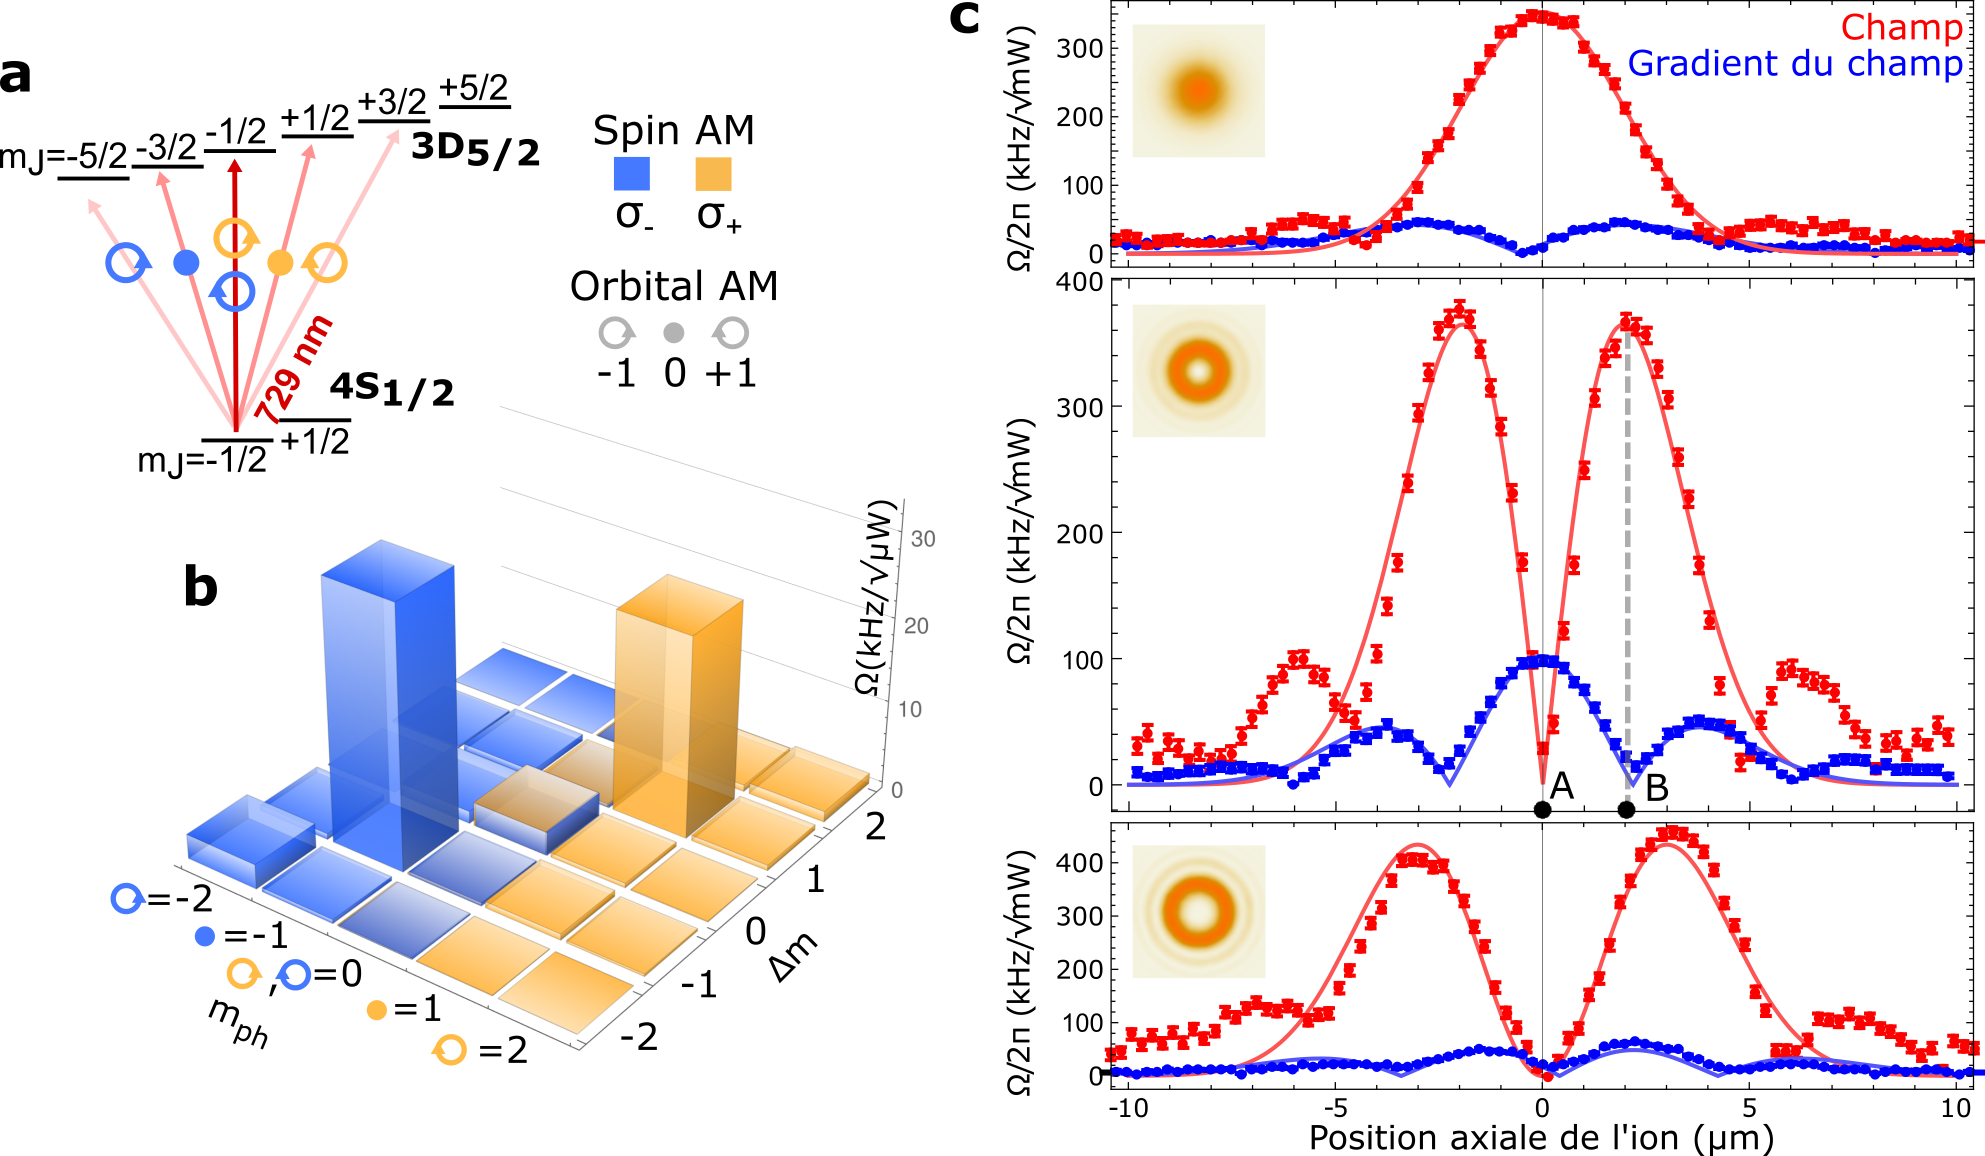
\includegraphics[width=0.9\columnwidth]{Figures/schmiegelow.png}
\caption{Observation de transition quadripolaire. (a) Transitions possibles mettant en jeu le MAS et le MAO. (b) Amplitudes de transition mesurées en utilisant une oscillation de Rabi. (c) Amplitude de transition dipolaire (rouge) et quadripolaire (bleu) en fonction de la position transverse de l'ion. Ces amplitudes sont reliées respectivement à l'amplitude du champ et du gradient du champ.}
\label{Fig:Schmiegelow}
\end{figure}


Nous avons maintenant terminé cette partie sur le concept de moment angulaire de la lumière. Nous avons introduit les définitions nécessaires et construit des champs électromagnétiques réalisables en pratiques dans lesquelles le moment angulaire est contrôlé. Dans le chapitre III, nous étudierons expérimentalement la génération de modes de Laguerre-Gauss à partir d'un laser infrarouge Gaussien, avant d'utiliser ces modes pour générer des harmoniques d'ordre élevé. Dans le chapitre IV, nous nous intéresserons au cas du moment angulaire de spin, c'est-à-dire de faisceaux polarisés circulairement. Nous chercherons à générer des harmoniques d'ordre élevé polarisées circulairement et à les utiliser dans l'étude de molécules chirales.
%\chapter{Le moment angulaire orbital dans la génération d'harmoniques d'ordre élevé}
\label{CH:OAM_HHG}
%
\section{Revue des utilisations pratiques des modes de Laguerre-Gauss}
\subsection{Le domaine visible et infrarouge}
\subsection{De plus courtes longueurs d'ondes : perspectives d'applications dans l'extrême ultra-violet}
\subsection{Des durées ultra-brèves : utilisations possibles d'impulsions attosecondes portant du moment angulaire orbital}

\section{Génération d'harmoniques d'ordre élevé à partir de modes de Laguerre-Gauss}

Ayant passé en revue les utilisations envisagées de faisceaux de Laguerre-Gauss de durées ultra-brève et dans le domaine de l'extrême ultra-violet (XUV), nous décrirons ici comment les générer de manière expérimentale. Nous commencerons par détailler notre dispositif de génération d'harmoniques d'ordre élevé dans le cas habituel d'un mode laser Gaussien, puis expliquerons comment passer au cas Laguerre-Gaussien avant de donner les résultats obtenus.

\subsection{Le cas Gaussien : Aspects expérimentaux de la génération d'harmoniques d'ordre élevé}
\label{Sec:HHG_G}
\subsubsection{Système laser}
Toutes les expériences présentées dans ce chapitre ont été réalisées sur le laser LUCA (Laser Ultra-Court Accordable) du LIDYL au CEA Saclay. Il délivre des impulsions ayant une enveloppe temporelle gaussienne de largeur à mi-hauteur $\tau = 50$ fs et une enveloppe spatiale gaussien de largeur à mi-hauteur $w_0 = 15$ mm à $\frac{1}{e^2}$. La longueur d'onde utilisée est 800 nm, et le taux de répétition est de 20 Hz. Ce système dispose d'une fibre utilisée pour filtrer spatialement le faisceau, ce qui garantit un profil très proche d'un mode gaussien pur \mycite{MahieuAPB2015}. Le prix à payer est une diminution de l'énergie par impulsion, qui atteint quand même environ 35 mJ après la fibre et le dernier étage de compression.

\subsubsection{Génération d'harmoniques d'ordre élevé}
Nous commençons par mettre en forme le faisceau laser : son diamètre est ajusté à l'aide d'un iris et son énergie est ajustée grâce à un atténuateur constitué d'une lame demi-onde et d'une paire de polariseur croisés. \`{A} la sortie de cet atténuateur, la polarisation du laser est verticale (S). Le faisceau est ensuite focalisé par une lentille dans un jet de gaz délivré par une vanne pulsée à la fréquence du laser par un système piezo-électrique (Attotech). L'utilisation d'une vanne pulsée permet de n'envoyer du gaz que lorsque le faisceau laser est présent, ce qui limite la pression résiduelle dans les chambres à vide. Ainsi, on peut atteindre une pression assez élevé (XXX) dans la région focale sans que l'émission harmonique ne soit réabsorbée par le gaz résiduel. Un autre paramètre important est le diamètre de l'orifice de la vanne (ici, 150 $\mu m$) : en choisissant un diamètre faible, on crée une extension supersonique du gaz ce qui garantit une longueur d'interaction faible avec le laser. On s'approche ainsi des conditions idéales d'un plan d'atomes, ce qui limite l'importance des effets d'accord de phase dans la GHOE. \par
Le choix du gaz dépend de l'expérience réalisée : on peut par exemple utiliser une molécule dont on étudie la réponse, on parle alors de spectroscopie harmonique. Le gaz n'est pas l'objet d'étude dans notre cas, on préférera donc choisir un système simple, facile à se procurer, et ayant une grande section efficace. Le gaz le plus courant est l'Argon, qui est peu coûteux et génère de manière très efficace. Son potentiel d'ionisation est de 15.76 eV, ce qui donne une énergie de coupure assez faible et qui empêche de générer des ordres harmoniques très élevés. Dans les cas où on désire générer des ordres élevés et nombreux, on pourra utiliser d'autres gaz rares comme le Néon ($I_p$ = 21.6 eV) même si la génération sera moins efficace.

Pour notre système, les paramètres nominaux sont :
\begin{itemize}
\item Le diamètre avant focalisation \O{} $\approx$ 10-15 mm,
\item L'énergie par impulsion de l'ordre de E = 1 mJ,
\item La lentille de longueur focale f = 1 m. \\
\end{itemize}
Pour calculer la valeur de l'intensité pic au foyer, on peut calculer le profil du faisceau après focalisation, par exemple par un calcul numérique. Le champ avant la lentille est défini dans les coordonnées cylindriques $(R,\theta)$ par :
\begin{equation*}
E(R,\theta) = \sqrt{I_0} \exp{\left(-\frac{R^2}{w_0^2}\right)}\times\delta(\frac{\mbox{\O}}{2}-R),
\end{equation*}
où $w_0$ est la largeur du faisceau collimaté avant l'iris, \O{}  est le diamètre de l'iris, $\delta$ est la fonction de Heaviside, et $I_0 = \frac{2E\sqrt{\frac{4\log{2}}{\pi}}}{\tau\pi w_0^2}$.
La focalisation d'un faisceau par une lentille mince peut être calculée par une transformée de Fourier (voir \mycite{Goodman}, un des ouvrages de référence pour l'optique de Fourier, et \mycite{Tan} pour des exemples d'implémentations numériques). Il est alors simple de voir l'effet des différents paramètres expérimentaux. Par exemple, on peut faire varier le diamètre de l'iris : la Figure \ref{Fig:IrisScan} montre le profil du faisceau au foyer quand \O{} varie entre 5 et 25 mm. On voit alors que l'intensité pic au foyer évolue entre 0 et 10 $\times 10^{14} \mbox{W/cm}^2$. On se trouve donc parfaitement dans le régime d'intensité nécessaire à la génération d'harmonique : l'intensité est suffisante pour enclencher une ionisation tunnel mais reste assez faible pour ne pas ioniser et dépléter tout le milieu.

\begin{figure}[!ht]
\centering
\def\svgwidth{\columnwidth}
\import{Figures/Iris_Scan/}{Fig_IrisScan.pdf_tex}
\caption{\'{E}volution du foyer lorsqu'on varie la taille de l'iris. De gauche à droite : (1) profil transverse de l'intensité au foyer, (2) intensité pic, (3) taille du waist. Les paramètres sont les suivants : E = 1 mJ, $w_0$ = 15 mm, $\tau$ = 50 fs, $\lambda$ = 792 nm, f = 1 m et \O{} variant de 5 à 25 mm par pas de 1 mm. Le calcul est réalisé sur une grille de 1025x1025 points correspondant à une taille réelle de 5*\O{}.}
\label{Fig:IrisScan}
\end{figure}

Les harmoniques d'ordre élevé du laser infrarouge sont ainsi générées par le gaz situé près du foyer de la lentille. Ce rayonnement XUV est ensuite ré-imagé par un dispositif composé de deux optiques :
\begin{enumerate}
\item Un miroir torique en or de 50 cm de focale. Le miroir travaille à $11.5\degres$ d'incidence rasante ($78.5\degres$ si on défini l'angle par rapport à la normale au miroir), ce qui permet d'avoir une réflectivité importante et plate sur la gamme spectrale considérée (voir Figure \ref{Fig:TorR}).

\begin{figure}[!ht]
\centering
\def\svgwidth{0.6\columnwidth}
\import{Figures/Reflect_Torique/}{torR.pdf_tex}
\caption{Réflectivité calculée du miroir torique en or à un angle d'incidence de $11.5\degres$. (CXRO, \mycite{Henke1993}).}
\label{Fig:TorR}
\end{figure}

Le miroir toroïdal est positionné dans une configuration 2f-2f de sorte à garder un rapport 1:1 entre le foyer de génération et le second foyer. Ré-imager le foyer de génération est utile car on peut focaliser le rayonnement harmonique dans un deuxième dispositif, comme par exemple un spectromètre à temps de vol dans le cas d'une mesure RABBIT (voir ChapitreXX et YY). Un autre avantage est qu'il éloigne la zone de génération, où la pression est élevée, de la zone de détection, qui requiert souvent un vide de qualité pour que les détecteurs fonctionnent.\\

\item La deuxième optique est une lame de Si$\mbox{O}_{\mbox{2}}$, qui réalise le rôle de filtrage de l'infrarouge de génération. La lame de silice est traitée antireflet pour l'infrarouge grâce à un dépôt de multicouches. La dernière de ces couches est en silice, ce qui combiné à une bonne qualité de surface permet de réfléchir efficacement le rayonnement harmonique. La Figure \ref{Fig:SilR}, tirée de \mycite{MairessePhD} présente la réflectivité de la lame pour le rayonnement harmonique et infrarouge. La réflectivité dans l'XUV est donc supérieure à 50\% jusqu'à l'ordre $\approx 37$, tandis que moins de 10\% de l'infrarouge est réfléchi. Le filtrage de l'infrarouge de génération est souvent crucial : il constitue un bruit de mesure non négligeable, sans compter qu'il peut facilement endommager des optiques ou des détecteurs en aval s'il est focalisé.

\begin{figure}[!ht]
\centering
\def\svgwidth{\columnwidth}
\import{Figures/Reflect_Silice/}{silR.pdf_tex}
\caption{Réflectivité de la lame de silice. \`{A} gauche, transmission et réflectivité à 800 nm en fonction de l'angle d'incidence rasante. Les pointillés repèrent notre angle de $11.5\degres$. \`{A} droite, réflectivité XUV mesurée (cercles) et donnée par le CXRO (lignes) (\mycite{Henke1993}). Figure adaptée de \mycite{MairessePhD}.}
\label{Fig:SilR}
\end{figure}
\end{enumerate}

Nous souhaiterions ensuite pouvoir imager le spectre harmonique, c'est-à-dire séparer les différents ordres harmoniques et mesurer leurs propriétés spatiales. Un peu après le second foyer, les harmoniques sont dispersées par un réseau à pas variable Hitachi 001-0437 (voir \mycite{KitaAO1983} pour des détails sur son fonctionnement). L'angle de réflexion d'un rayonnement monochromatique de longueur d'onde $\lambda$ est donné par la formule des réseau :
\begin{equation*}
m\lambda=\frac{\sin{\alpha}+\sin{\beta}}{\sigma},
\end{equation*}
où $m$ est l'ordre de diffraction considéré (généralement 1), $\sigma$ le nombre de trait par mètre (1200 traits/mm dans notre cas), $\alpha$ et $\beta$ les angles d'incidence et de réflexion, définis par rapport à la normale au réseau (la documentation donne $\alpha = 87$\degres{} pour un fonctionnement optimal).\par
Le réseau de diffraction est cylindrique : il est focalisant dans la dimension horizontale mais est plan dans la direction verticale. Un rayonnement gaussien de faible largeur spectrale $\Delta\lambda$ et de largeur spatiale $w(z)$ formera donc dans le plan focal du réseau une fine ligne verticale de largeur proportionnelle à $\Delta\lambda$ et de hauteur $w(z)$. On image ainsi à la fois les dimensions spectrale et spatiale, si on suppose la symétrie cylindrique. Ce spectre est imagé par des galettes de micro-canaux couplées à un écran de phosphore, lui-même observé par une caméra CCD Basler A102f. 

L'intégralité du dispositif expérimental est représenté sur la Figure \ref{Fig:ExpG}.
\newpage
\vspace{\baselineskip}
\begin{figure}[!ht]
\centering
\def\svgwidth{\columnwidth}
\import{Figures/Setup_G/}{setupG_wbitmap.pdf_tex}
\caption{Dispositif expérimental de génération et détection d'harmoniques d'ordre élevé.}
\label{Fig:ExpG}
\end{figure}

Les figures \ref{Fig:SpectrumGAr} et \ref{Fig:SpectrumGNe} présentent des spectres obtenus avec ce dispositif en utilisant respectivement l'argon et le néon comme gaz de génération. On observe les ordres harmoniques allant de 13 à 29 dans l'argon, et de 13 à 57 dans le néon, la différence d'énergie de coupure étant attendue puisque le néon a un $I_p$ plus élevé. Sur le spectre de l'argon, on observe clairement les deux trajectoires quantiques de la GHOE : une contribution sur l'axe correspond à la trajectoire courte et une plus divergente et moins intense correspond à la trajectoire longue. Dans le cas du néon, les conditions d'accord de phase utilisées favorisent la trajectoire courte. On remarque également que la divergence de la trajectoire courte (resp. longue) augmente (rep. diminue) avec l'ordre harmonique, jusqu'à ce que les deux trajectoires se confondent dans la coupure. Notons finalement la présence sur le spectre du néon de pics satellites autour des harmoniques les plus basses : il s'agit des harmoniques plus élevées diffractées au second ordre par le réseau.
\begin{figure}[!ht]
\centering
\def\svgwidth{\columnwidth}
\import{Figures/Spectrum_G/}{Spectrum_G_Ar.pdf_tex}
\caption{Spectre d'harmoniques d'ordre élevé générées dans l'argon à partir d'un mode laser gaussien.}
\label{Fig:SpectrumGAr}
\end{figure}
\begin{figure}[!ht]
\centering
\def\svgwidth{\columnwidth}
\import{Figures/Spectrum_G/}{Spectrum_G_Ne.pdf_tex}
\caption{Spectre d'harmoniques d'ordre élevé générées dans le néon à partir d'un mode laser gaussien.}
\label{Fig:SpectrumGNe}
\end{figure}

\subsection{Génération de modes de Laguerre-Gauss dans le visible et proche infrarouge}
Ayant décrit la génération ``habituelle'' d'harmoniques d'ordre élevé, décrivons maintenant l'expérience où le laser générateur possède un mode de Laguerre-Gauss, dont l'expression a été donnée au chapitre précédent (équation \ref{eq:lgmodes}). Les modes de Laguerre-Gauss possèdent un moment angulaire orbital bien défini grâce à leur phase hélicoïdale. Plus précisément, c'est le terme $e^{\rmi\ell\theta}$, également présent dans les modes de Bessel, qui leur confère cette propriété. Il sera question de l'index radial $p$ des modes de Laguerre-Gauss plus loin dans cette thèse, mais il n'a pour l'instant pas d'importance pour notre problème. La première question est donc de savoir comment produire un mode de Laguerre-Gauss d'index $(\ell_{IR},0)$ dans l'infrarouge. 

\subsubsection{Superposition de modes de Hermite-Gauss}
\label{sec:hg_modes}
Les faisceaux de LG étant des modes du champ électromagnétique, on peut d'abord penser à modifier le laser lui-même pour qu'il lase directement dans le mode désiré. En introduisant des éléments absorbants dans la cavité, il est a priori possible d'interdire la génération d'un mode Gaussien. En pratique, il est assez compliqué de sélectionner un mode de LG. Il est par contre assez simple de sélectionner un des modes de \textit{Hermite-Gauss}, qui sont les solutions de l'équation d'onde en coordonnées cartésiennes. Ces modes sont souvent appelés modes $\mbox{TEM}_{nm}$, pour ``Transverse Electro-Magnetic'', dont le mode Gaussien $\mbox{TEM}_{00}$ n'est simplement que le mode d'index le plus bas. Quelques uns de ces modes sont représentés sur la figure \ref{Fig:hgmodes}. En insérant simplement un fil vertical (resp. horizontal) dans la cavité laser, on bloque la génération du $\mbox{TEM}_{00}$ et on obtient un mode $\mbox{TEM}_{01}$ (resp. $\mbox{TEM}_{10}$).

\begin{figure}[!ht]
\centering
\def\svgwidth{\columnwidth}
\import{Figures/Mode_Converter/}{HG_Modes.pdf_tex}
\caption{Modes de Hermite-Gauss pour différentes valeurs de $(n,m)$. De gauche à droite, $(n,m) =$ (0,0), (1,0), (0,1), (2,0), (2,1), (3,3). Le code couleur est le même que celui de la figure \ref{Fig:LGModes} : la couleur donne la phase et la luminosité l'intensité.}
\label{Fig:hgmodes}
\end{figure}

Les faisceaux de Hermite-Gauss constituent également une base des modes du champ, dans laquelle on peut donc écrire les modes de Laguerre-Gauss. On peut montrer (\mycite{BeijersbergenOC1993}) que les composantes du mode $\mathcal{LG}_{\ell,p}$ sont égales aux composantes d'un mode $\mbox{TEM}_{nm}$ incliné à 45\degres{} avec $p = \mathrm{min}(m,n)$ et $\ell=m-n$, la seule différence étant l'ajout d'une phase de $\pi/2$ entre les différentes composantes successives. Par exemple pour $\ell = 1$,
\begin{align*}
\mbox{TEM}_{n,m}^{45\mbox{\degres}}&=\frac{1}{\sqrt{2}}\mbox{TEM}_{01}+\frac{1}{\sqrt{2}}\mbox{TEM}_{10} \mbox{ et}\\
\mathcal{LG}_{1,0}&=\frac{1}{\sqrt{2}}\mbox{TEM}_{01}+\frac{\rmi}{\sqrt{2}}\mbox{TEM}_{10}.
\end{align*}
Pour $\ell = 2$, 
\begin{equation*}
\mathcal{LG}_{2,0}=\frac{1}{2}\mbox{TEM}_{02}+\frac{\rmi}{\sqrt{2}}\mbox{TEM}_{11}-\frac{1}{\sqrt{2}}\mbox{TEM}_{20}
\end{equation*}
et ainsi de suite.
Comme dit plus haut, il est possible de générer un mode $\mbox{TEM}_{n,m}$ en cavité, il reste seulement à l'incliner à 45\degres par rapport au repère choisi. Pour contrôler la phase entre les composantes relatives, les auteurs de \mycite{BeijersbergenOC1993} ont montré qu'on pouvait utiliser des lentilles cylindriques. En effet, une lentille cylindrique convergente ne focalise qu'une seule des composantes cartésiennes, qui va subir un déphasage au passage du foyer dû à la phase de Gouy. On recollimate ensuite le faisceau avec une deuxième lentille cylindrique de même focale $f$. La phase ajoutée est ajustée en changeant la distance entre ces deux lentilles; pour obtenir $\pi/2$ il faut choisir $\sqrt{2}f$. La Figure \ref{Fig:Modeconv} illustre le principe de ce dispositif, appelé convertisseur de mode.

\begin{figure}[!ht]
\centering
\def\svgwidth{0.5\columnwidth}
\import{Figures/Mode_Converter/}{mode_converter.pdf_tex}
\caption{Schéma de fonctionnement d'un convertisseur de mode : en partant d'un $\mbox{TEM}_{01}$ incliné à 45\degres, on obtient un mode $\mathcal{LG}_{1,0}$. Tiré de \mycite{PadgettAllen1999}.}
\label{Fig:Modeconv}
\end{figure}

L'intérêt de ce dispositif est de créer des modes purs : on obtient exactement le faisceau de Laguerre-Gauss recherché. Il présente cependant deux inconvénients : (1) il faut disposer d'un mode $\mbox{TEM}_{0\ell}$ au départ, ce qui devient compliqué dès que $\ell$ augmente. De plus, il est peu pratique de devoir modifier la cavité laser, particulièrement dans le cas des lasers de puissances utilisés pour la HHG. (2) Le faisceau est focalisé dans une dimension entre les deux lentilles. La puissance fournie par notre laser imposerait de réaliser la conversion dans une enceinte à vide, sans quoi la focalisation dans l'air détruira le profil spatial et temporel du faisceau. Pour ces raisons, nous avons choisi une méthode plus flexible et plus adapté à un laser de puissance.

\subsubsection{Utilisation d'une lame de phase à spirale}
Cette technique est probablement la façon la plus intuitive d'ajouter le terme de phase qui nous intéresse au faisceau. Pour rajouter une phase $e^{\rmi\ell\theta}$, il suffit d'utiliser une lame de verre transparente dont l'épaisseur varie proportionnellement à $\theta$. On forme ainsi une \textit{lame de phase à spirale} (Spiral Phase Plate, SPP), concept proposé dans \mycite{BeijersbergenOC1994} et représenté sur la Figure \ref{Fig:SPP}.\par
\begin{figure}[!ht]
\centering
\def\svgwidth{0.5\columnwidth}
\import{Figures/SPP/}{SPP.pdf_tex}
\caption{Lame de phase à spirale. La flèche rouge représente le trajet d'un rayon optique. Adapté de \mycite{YaoAOP2011}.}
\label{Fig:SPP}
\end{figure}
La lame présente une discontinuité pour $\theta=0$\degres, dont la hauteur h permet de contrôler le moment angulaire orbital transféré au faisceau pour une longueur d'onde donnée. Si cette hauteur est assez faible pour que l'on reste dans le régime paraxial, on peut considérer que la lame agit uniquement sur la phase du faisceau incident. Ainsi si on choisit 
\begin{equation*}
h = \frac{\ell\lambda}{n-1},
\end{equation*}
où $n$ est l'indice de réfraction du milieu, pour un champ d'entrée $u(r,\theta,z)$ on obtient directement après la lame $u' = u\exp{(-\rmi \ell \theta)}$.	Il est donc non seulement possible de passer d'un mode Gaussien à un mode Laguerre-Gaussien, mais encore de changer l'indice d'un mode déjà Laguerre-Gaussien.\par
La lame de phase illustre joliment la création de MAO : si on considère une onde plane arrivant perpendiculairement à la surface plane de la lame, le rayon qui sort de la lame sera dévié par réfraction à travers la surface hélicoïdale. Cette réfraction se fait dans la direction azimutale, le moment linéaire de la lumière acquière donc une composante azimutale, synonyme de moment angulaire. Plus précisément, pour un rayon $r$ donné, l'angle de la surface	vaut $h/(2\pi r)$. Si on applique la loi de Snell-Descartes on obtient que le rayon est dévié d'un angle $\alpha = (n-1)\ell\lambda/(2\pi r(n-1)) = \ell/(k_0r)$. Le moment linéaire par photon vaut $\hbar k_0$, donc le moment angulaire par photon vaut $r\times\hbar k_0\times\ell/(k_0r) = \ell\hbar$.


Si le principe d'une SPP est simple, sa construction est beaucoup plus compliquée. Les tolérances sur la valeur de h et la régularité de la surface sont très strictes aux longueurs d'ondes optiques, sans quoi la qualité du mode de sortie sera détériorée (si h n'est pas adapté, on peut même créer des modes d'indice non entier, cf. \mycite{LeachNJP2004}). D'ailleurs, lors des premiers travaux sur le sujet (\mycite{BeijersbergenOC1994}), la température de la lame était ajustée pour accorder précisément la hauteur de la lame à la longueur d'onde. La technique a évolué et il est maintenant possible de créer des SPP de très bonne qualité \mycite{OemrawsinghAO2004}.

Enfin, remarquons que même pour une SPP parfaite, la conversion d'un mode à l'autre n'est jamais idéale. La SPP agit sur la phase du faisceau, mais ne modifie pas le profil d'intensité. Ainsi, à sa sortie le champ électrique a la bonne phase mais pas la distribution d'intensité d'un mode de Laguerre-Gauss (termes sur la première ligne de l'équation \ref{eq:lgmodes}). La conséquence est que le champ $u_{exp}$ créé n'est pas un mode pur du champ, mais une superposition de modes de Laguerre-Gauss de différents indices. Ainsi, son intensité sera fortement modulée au cours de la propagation selon la phase entre ces différents modes. Le cas qui nous intéresse principalement est la conversion d'un mode Gaussien vers un mode LG. Dans ce cas, cette superposition s'écrit :
\begin{align}
\begin{split}
u_{exp}(r,\theta,z) &= \sum_{p=0}^\infty\sum_{\ell=-\infty}^\infty{\Braket{u_{exp}(r,\theta,z)|\mathcal{LG}_{\ell,p}(r,\theta,z)} \ket{\mathcal{LG}_{\ell,p}(r,\theta,z)}}\\
&=\sum_{p=0}^\infty\sum_{\ell=-\infty}^\infty{\Braket{TEM_{00}(r,\theta,z)\cdot e^{\rmi\ell'\theta}|\mathcal{LG}_{\ell,p}(r,\theta,z)} \ket{\mathcal{LG}_{\ell,p}(r,\theta,z)}},
\end{split}
\label{Eq:decompLG}
\end{align}
où $\ell'$ est l'indice azimutal correspond à la hauteur de la SPP. Les coefficients sont simplement donnés par le produit scalaire ci-dessus. On remarque qu'il a la forme suivante :
\begin{equation*}
\Braket{TEM_{00}(r,\theta,z)\cdot e^{\rmi\ell'\theta}|\mathcal{LG}_{\ell,p}(r,\theta,z)} = \int_{r=0}^\infty\int_{\theta=0}^{2\pi}{\ldots \; e^{\rmi(\ell'-\ell)\theta}r\rmd r \rmd \theta},
\end{equation*}
l'intégrale selon $\theta$ s'annule donc dès que $\ell\neq\ell'$. Les modes de la superposition ont donc tous le même index azimutal mais des $p$ différents. Ces coefficients peuvent être calculés numériquement, par exemple \mycite{BeijersbergenOC1994} obtiennent pour le cas $\ell' = 1$ les valeurs présentées dans le Tableau \ref{Tab:DecompBei}. On conclut donc que le faisceau est composé majoritairement du mode $\mathcal{LG}_{1,0}$. Les valeurs deviennent moins bonne lorsqu'on augmente $\ell$, par exemple un Gaussien passant à travers une lame dessinée pour ajouter $\Delta\ell =2$ n'est composé qu'à 50\% du mode $\mathcal{LG}_{2,0}$ recherché.
\begin{center}
  \begin{tabular}{ c | c | c | c | c | c | c }
    \hline
		& $p = 0$ & 1 & 2 & 3 & 4 & 5 \\ \hline
    $\ell=1$ & 78.5 & 9.82 & 3.68 & 1.92 & 1.17 & 0.79 \\ \hline
  \end{tabular}
	\caption{Décomposition du champ obtenu en passant un mode Gaussien pur à travers une lame de phase à spirale. D'après \mycite{BeijersbergenOC1994}.}
	\label{Tab:DecompBei}
\end{center}
Pour finir, mentionnons une technique permettant de relâcher un peu les contraintes de fabrication d'une SPP : il est possible de discrétiser la pente de phase, ce qui rend la lame plus facile à construire et donc plus accessible. Cette technique est détaillée dans \mycite{SuedaOE2004}, où les auteurs calculent l'influence du nombre de points de discrétisation sur la pureté modale obtenue :
\begin{center}
  \begin{tabular}{c | c | c | c | c | c}
    \hline
		Nombre de points de discrétisation & $\infty$ & 32 & 16 & 8 & 4 \\ \hline
    Efficacité $\mathcal{LG}_{0,0}\rightarrow\mathcal{LG}_{1,0}$ & 78.5 & 78.3 & 77.5 & 74.6 & 63.7 \\ \hline
  \end{tabular}
	\caption{Efficacité de conversion d'une lame de phase à spirale $\Delta\ell=1$ en fonction du niveau de discrétisation. D'après \mycite{SuedaOE2004}.}
	\label{Tab:DecompSueda}
\end{center}
La qualité du mode obtenue est donc très correcte même jusqu'à 8 niveaux. Les auteurs montrent également que ces lames de phase sont adaptées à des utilisations avec des faisceaux courts et intenses, contrairement à la plupart des autres méthodes. Pour ces raisons, nous avons finalement choisi d'utiliser une lame de phase discrétisée sur 16 niveaux, et disposons de lames $\Delta\ell = 1$ et $\Delta\ell = 2$ à 800 nm, ce qui nous permet d'aller jusqu’à $\ell = 3$ en les mettant l'une après l'autre.

\subsubsection{Résultats expérimentaux sur la création de modes de Laguerre-Gauss dans l'infrarouge}
Même si le système laser a été décrit plus haut, notons encore une fois l'importance du filtrage spatial installé sur notre chaîne : il nous garantit un mode Gaussien très pur, ce qui favorise grandement la création de modes Laguerre-Gaussien de qualité. \par
Les lames de phases utilisées ont été construites par la société Silios Technologies et font 17 mm de diamètre. Elle ou elles sont insérées directement après l'iris et avant la lentille. Le faisceau étant bien collimaté, nous n'avons pas observé de différence notable selon le placement de la lame. Il est intéressant d'observer l'intensité du faisceau un peu après le passage dans la lame : 

\begin{figure}[!ht]
\centering
\def\svgwidth{0.4\columnwidth}
\import{Figures/SPP/}{Beam_1m_After_SPP.pdf_tex}
\caption{Intensité transverse après être passée dans une lame de phase à spirale $\Delta\ell = 1$. Le faisceau est d'abord diaphragmé par un iris de diamètre 10 mm, la distance d'observation après la lame est de 1 m.}
\label{Fig:BeamAfterSPP}
\end{figure}

On observe 16 ``pétales'' sur les bords du faisceau, qui correspondent à la diffraction par les 16 marches de la lame. On voit également la singularité de phase déjà formée, qui donne un zéro d'intensité au centre. Clairement, l'intensité du faisceau est encore très loin de celle d'un mode de Laguerre-Gauss : il n'y a que dans le champ lointain que le faisceau prendra la forme désirée. Dans notre cas, cela se passe au foyer de la lentille de génération. Nous imageons ce foyer à l'aide d'une caméra CCD Imagine Source équippée d'un objectif x5 et d'un tube de 160 mm. La figure \ref{Fig:LGFocus} présente les résultats obtenus.\par
\begin{figure}[!ht]
\centering
\def\svgwidth{0.8\columnwidth}
\import{Figures/IRFocus/}{SPP1focus.pdf_tex}
\caption{Intensité laser au foyer d'une lentille de 1m, après passage à travers (1) une lame de phase $\Delta\ell = 1$, (2) une lame de phase $\Delta\ell = 2$, et (3) les deux lames placées successivement.}
\label{Fig:LGFocus}
\end{figure}
On mesure le diamètre de l'anneau, défini comme la distance entre les deux maxima d'intensité le long d'une ligne radiale, et on obtient 200, 280 et 400 \si{\um} pour $\ell=$1, 2, 3. Ceci est cohérent avec la dépendance en $\sqrt{\ell}$ attendue (voir équation \ref{Eq:rmax_LG}), mais ne constitue pas une mesure directe du MAO porté par le faisceau. Pour ce faire, il existe de nombreuses techniques développées dans le domaine visible et infrarouges dont le but est toujours de révéler le terme de phase $\mathrm{e}^{\rmi\ell\theta}$. Pour révéler cette phase spatiale, il est naturel d'essayer d'observer des interférences, soit avec un autre faisceau - l'interférence avec un gaussien donne une ``fourche'' d'ordre $\ell$ \mycite{bazhenov1990} - ou bien du faisceau avec lui même, c'est-à-dire sa diffraction. De nombreux objets diffractifs ont été utilisés, par exemple une fente \mycite{ghai2009} ou des fentes de Young \mycite{sztul2006}, avec lesquelles le signe et la parité de $\ell$ se retrouvent dans le décalage des franges, ou bien des objets plus compliqués tels que des grilles de pupilles \mycite{berkhout2008} qui donnent directement la valeur de $\ell$. On peut également mentionner les ouvertures bloquant une partie angulaire du faisceau, ce qui se répercute sur le contenu modal du faisceau à travers la relation d'incertitude $\Delta\ell\Delta\phi > K$ déjà mentionnée (TODO). Certaines méthodes sont généralisables au cas d'un photon unique et ont permis de mesurer de l'intrication entre différents états de moment orbital angulaire \mycite{MairNature2001} ainsi qu'un équivalent angulaire au paradoxe EPR \mycite{LeachScience2010}. \par 
Nous avons choisi d'utiliser une ouverture en triangle, qui donne une figure de diffraction assez surprenante : on obtient une grille de points diffractés en forme de triangle, dont l'orientation donne le  signe de $\ell$ alors que le nombre de points donne $\left|\ell\right|$ : sur l'arête extérieure au triangle, on a $\left|\ell\right|+1$ points \mycite{HickmannPRL2010}. Après être passé dans la SPP, le faisceau est diffracté par une ouverture triangulaire dont la taille est ajustable à l'aide d'un système motorisé conçu par M. Bougeard. On choisit l'ouverture de l'ordre du waist du faisceau, ce qui permet d'observer la figure de diffraction en imageant le foyer d'une lentille de focale f=1m. La figure \ref{Fig:Triangle} illustre le principe et les résultats de cette expérience. 

\begin{figure}[!ht]
\centering
\def\svgwidth{1.0\columnwidth}
\import{Figures/Triangle/}{triangle.pdf_tex}
\caption{Mesure directe du moment angulaire orbital porté par le faisceau infrarouge à l'aide d'une ouverture triangulaire.}
\label{Fig:Triangle}
\end{figure}

Nous avons pu vérifier la validité de cette méthode pour des moments angulaires plus élevés. Pour les obtenir, le champ infrarouge $E_{800}$ est doublé à l'aide d'un cristal de BBO (bêta-borate de baryum). On obtient un champ à 400 nm, dont l'amplitude est donné par la loi habituelle de l'optique non-linéaire perturbative $E_{400}\propto E_{800}^2\propto \rme^{2\rmi\ell_{IR}\theta}$. Le MAO du faisceau est ainsi doublé, comme vérifié expérimentalement par \mycite{DholakiaPRA1996}. Les résultats obtenus après diffraction par la fente triangulaire sont présentés sur la figure \ref{Fig:Triangle400}. 

\begin{figure}[!ht]
\centering
\def\svgwidth{0.5\columnwidth}
\import{Figures/Triangle/}{triangle400.pdf_tex}
\caption{Mesure directe du moment angulaire orbital porté par le champ obtenu après doublage du faisceau infrarouge dans un cristal de BBO.}
\label{Fig:Triangle400}
\end{figure}

Ceci constitue donc une preuve directe que le faisceau est composé très majoritairement du mode $\mathcal{LG}_{\ell,0}$. Bien sûr, on ne s'attend quand même pas à ce que les modes obtenus soient purs, du fait de la lame de phase mais également à cause de l'iris qui limite la dimension transverse du faisceau. On peut évaluer numériquement l'effet de tous ces éléments : on effectue un calcul de propagation de la même façon qu'expliqué en page \pageref{Fig:IrisScan}, cette fois en rajoutant l'effet de la lame de phase discrète. Une fois le foyer obtenu, on calcule sa décomposition dans la base des modes de Laguerre-Gauss en évaluant numériquement les coefficients du type \ref{Eq:decompLG}. Comme noté page \pageref{Eq:rmax_LG}, les modes de Laguerre-Gauss ne constituent une base que pour une valeur de $w(z)$ donnée. Il faut donc choisir cette valeur avant d'effectuer la décomposition. On fait l'hypothèse que le mode obtenu est assez proche d'un mode pur $(\ell,0)$ pour que son rayon soit donné par l'équation \ref{Eq:rmax_LG}, ce qui nous permet de fixer $w(z)$. La figure \ref{Fig:DecompIR} montre l'intensité au foyer et les coefficients de la décomposition ainsi obtenus. On voit que le foyer est composé du mode $\mathcal{LG}_{\ell,0}$ à 72, 48 et 42\% pour $\ell=1,2,3$ respectivement. On observe également l'apparition d'un deuxième anneau pour $\ell =2$ et 3, dû au vignetage du faisceau par l'iris et cohérent avec la présence de davantage de modes $p$. \par

\begin{figure}[!ht]
\centering
\def\svgwidth{\columnwidth}
\import{Figures/Mode_Decomposition_IR/}{mode_L123.pdf_tex}
\caption{Intensité laser au foyer d'une lentille de 1m, après passage à travers (1) une lame de phase $\Delta\ell = 1$, (2) une lame de phase $\Delta\ell = 2$, et (3) les deux lames placées successivement.}
\label{Fig:DecompIR}
\end{figure}

Nous concluons donc que même si le contenu modal devient moins pur à mesure que $\ell$ augmente, le mode dominant reste celui qui nous intéresse. La GHOE étant un processus très non-linéaire, c'est lui qui contribuera majoritairement. 

\subsection{Génération d'harmoniques d'ordre élevé d'un faisceau de Laguerre-Gauss}
\subsubsection{Contraintes expérimentales}
Une fois qu'on dispose d'un faisceau infrarouge de MAO défini, l'expérience ne diffère en principe pas du cas Gaussien présenté dans la partie \ref{Sec:HHG_G}. En pratique, un problème important subsiste : celui de l'intensité pic. Nous avons vu que pour générer des harmoniques d'ordre élevé, l'intensité au foyer doit être de l'ordre de $\SI{1e14}{W/cm^2}$. Pour un mode de Laguerre-Gauss d'index $(\ell,0)$, l'intensité maximale est obtenue en $r_\mathrm{max}$ (équation \ref{Eq:rmax_LG}) :
\begin{align*}
I_\ell(r_\mathrm{max},z=0) &= \frac{C_{\ell,0}^2}{{w_0}^2}{\left( {\frac{r_\mathrm{max}\sqrt{2}}{{w_0}}} \right)^{2\left| \ell  \right|}}{e^{\left( { - \frac{{2{{r_\mathrm{max}}^2}}}{{{{w_0}^2}}}} \right)}}\\
&= \frac{2}{\pi(1+\delta_{0\ell})\left| \ell  \right|!{w_0}^2}\ell^{\left| \ell  \right|}{e^{-\ell}}
\end{align*}
La formule de Stirling donne $\left| \ell  \right|!\approx\sqrt{2\pi\left| \ell  \right|}\left| \ell  \right|^{\left| \ell  \right|}e^{-\left| \ell  \right|}$. Elle est valable respectivement à 8\%, 4\% et 2.6\% près pour $\ell=1,\;2,\;3$. On peut donc approximer :
\begin{equation*}
I_\ell(r_\mathrm{max},z=0) \approx \frac{2}{\pi{w_0}^2}\frac{1}{\sqrt{2\pi\left| \ell  \right|}}\text{ pour }\ell\neq0. 
\end{equation*}  
L'intensité pic évolue donc en $1/\sqrt{\left| \ell  \right|}$, la génération est donc de plus en plus compliquée à mesure que le MAO de l'infrarouge $\ell_{IR}$ augmente. Si on évalue l'expression exacte ci-dessus, on obtient :

\begin{center}
  \begin{tabular}{ c | c | c | c | c }
    \hline
		$\ell_{IR}$ & 0 & 1 & 2 & 3 \\ \hline
    $I_{\mathrm{max}}$ & 1 & 0.7358 & 0.5413 & 0.4481 \\ \hline
  \end{tabular}
	\caption{Intensité pic d'un mode de Laguerre-Gauss en fonction de $\ell$. Les intensités sont normalisées à celle du mode $\ell = 0$.}
\end{center}
Nous avons la chance de disposer d'un laser assez énergétique (jusqu'à 35 mJ disponibles), qui comme on le verra est suffisant pour générer jusqu'à $\ell_{IR}=3$. Il est égalemen

La seconde contrainte expérimentale est due au système d'imagerie. Comme démontré plus haut, le faisceau infrarouge est constitué d'un mode de Laguerre-Gauss principal. Le principe de conservation du moment angulaire nous amène à penser que les harmoniques générées doivent également porter du MAO, et prendront donc problablement la forme de modes de Laguerre-Gauss. Nous avons vu dans la partie \ref{sec:hg_modes} que les modes de Laguerre-Gauss peuvent être vus comme la superposition de plusieurs modes d'Hermite-Gauss et que le déphasage entre ces modes était crucial. En particulier, le convertisseur de mode présenté sur la figure \ref{Fig:Modeconv} repose sur l'utilisation de lentilles cylindriques pour contrôler la phase d'un seul des modes de Hermite-Gauss. On comprend donc que n'importe quel élément optique focalisant différemment les deux composantes cartésiennes du champ va modifier la phase relatives des modes HG et détruire le mode de Laguerre-Gauss. Dans notre dispositif présenté sur la figure \ref{Fig:ExpG}, on trouve deux éléments problématiques :
\begin{itemize}
\item Les optiques de focalisation peuvent être astigmatiques. En particulier, la lentille de focalisation et le miroir torique doivent être alignés parfaitement, sans quoi notre mode en sera perturbé.\\
\item Le réseau de diffraction du spectromètre est un réseau cylindrique, il va donc systématiquement détruire le profil du faisceau au passage de son foyer. 
\end{itemize}

L'effet du réseau de diffraction cylindrique peut être calculé. Par exemple, \mycite{VaityPLA2013} proposent d'utiliser l'astigmatisme introduit par une lentille inclinée pour mesurer le MAO porté par un faisceau. Nous adaptons ici leur formalisme au cas de notre réseau de diffraction. Considérons par simplicité un faisceau collimaté incident sur le réseau de diffraction. Pour décrire sa propagation, on peut utiliser les matrices de transfert. La matrice totale du système est
\begin{equation*}
M_{\mathrm{tot}} = M_{z_1}\cdot M_{\mathrm{r\acute{e}seau}}\cdot M_{z_0}\;,
\end{equation*}
où $z_0$ est la distance de propagation en amont du réseau, $z_1$ la distance en aval, $M_z$ et $M_{\mathrm{r\acute{e}seau}}$ décrivent respectivement la propagation sur une distance $z$ et la focalisation par le miroir :
\begin{equation*}
M_z = \left(
\begin{array}{cc}
	I & zI \\
	0 & I
\end{array} \right)\text{ avec } 
I = \left(
\begin{array}{cc}
	1 & 0 \\
	0 & 1
\end{array} \right)
\end{equation*}


\begin{equation*}
M_{\mathrm{r\acute{e}seau}} = \left(
\begin{array}{cc}
	I & 0 \\
	-C/f & I
\end{array} \right)\text{ avec } 
C = \left(
\begin{array}{cc}
	1 & 0 \\
	0 & 0
\end{array} \right).
\end{equation*}
$f$ est la longueur focale effective du réseau dans la direction horizontale. En fonction nominal, le réseau focalise horizontalement les harmoniques dans un plan appelé ''spectral'' situé 235 mm en aval \mycite{KitaAO1983}. Comme on considère ici un faisceau collimaté, on prendra $f$ = 235 mm.
\`{A} partir de $M_{\mathrm{tot}}$, l'équation (8) de \mycite{VaityPLA2013} donne l'expression analytique du champ à une distance $z_1$ du réseau. On y trouve un terme Gaussien elliptique et sans surprise, un polynôme de Hermite. Pour évaluer cette expression, choisissons par exemple l'harmonique 11 et supposons qu'elle porte un moment angulaire orbital bien défini. Considérons qu'elle soit collimaté et que son waist soit égal à 10 mm. La figure \ref{Fig:gratingfocus} représente l'intensité obtenue pour $z_1$ variant autour de 235 mm, en supposant $\ell_{11} = 3$ ou 11. Nous voyons d'abord qu'à l'écart du foyer, l'anneau est simplement focalisé dans la dimension spectrale (noter les échelles différentes en $x$ et $y$), puis qu'au foyer le faisceau prend la forme d'un mode de Hermite-Gauss d'index $\ell_{11}$ tourné à 45$\deg$ par rapport à l'axe du réseau. On ne peut donc pas imager le spectre harmonique en ce point comme dans le cas Gaussien. Cependant, si on s'écarte trop du plan spectral du réseau, les harmoniques ne sont plus séparées spatialement. De plus, leur intensité est moindre, ce qui rend la mesure plus difficile. Le compromis finalement choisi est de placer le détecteur 8 cm en amont du plan focal, ce qui donne des harmoniques séparées et un effet cylindrique peu visible.

\begin{figure}[!ht]
\centering
\def\svgwidth{1.1\columnwidth}
\import{Figures/Gratingfocus/}{gratingfocus.pdf_tex}
\caption{Intensité de l'harmonique 11 au voisinage du foyer du réseau de diffraction cylindrique, en supposant $\ell_{11} = 3$ (ligne du haut) et $\ell_{11} = 11$ (ligne du bas). La position longitudinale $z$ est indiquée au dessus des images. La dimension verticale est celle non focalisée par le réseau, et est donc plusieurs ordres de grandeurs plus large que la dimension horizontale. Notons également que l'échelle horizontale change d'une image à l'autre, de sorte à garder une image résolue.}
\label{Fig:gratingfocus}
\end{figure}

La dernière contrainte expérimentale est celle de la divergence du faisceau 

\subsubsection{Résultats}
Nous présentons ici les spectres obtenus après les modifications expliquées ci-dessus effectuées. De plus, pour éviter que le



\section{Conservation du moment angulaire orbital dans la GHOE}
\subsection{Interprétation des résultats observés à partir de calculs analytiques}
\subsection{Simulations numériques de la propagation de modes de Laguerre-Gauss}
\subsection{Calculs SFA : une simulation complète de l'expérience réalisée}

\section{Rôle des trajectoires quantiques dans la GHOE à partir de faisceaux de Laguerre-Gauss}
\subsection{Observation des contributions des différentes trajectoires quantiques à partir des calculs numériques}
\subsection{Observation expérimentale de ces contributions}
\subsection{Interprétation des résultats obtenus : le rôle de l'index radial des modes de Laguerre-Gauss}

\section{Le profil spatio-temporel des impulsions générées : les ``light springs''}
\subsection{Mesure de la phase spectrale de l'impulsion à partir de la technique RABBIT}
\subsection{Reconstruction du profil spatio-temporel de l'émission}

\section{Contrôle complet du moment orbital angulaire de l'émission dans un schéma à deux faisceaux}
\subsection{Lois de conservations dans un schéma à deux faisceaux}
\subsection{Dispositif colinéaire}
\subsection{Dispositif non colinéaire}

\section{Le reste?}
\subsection{Le FEL?}
\partimage[width=1\columnwidth]{Figures/PartImages/FigCh4.png}
\part{Polarisation circulaire, molécules chirales et harmoniques d'ordre élevé}
\label{PA:Spin_HHG}
\chapter{Génération d'harmoniques d'ordre élevé polarisées elliptiquement}
\label{CH:Circular_HHG}
Dans cette partie nous présenterons comment générer des harmoniques d'ordre élevé portant du moment angulaire de spin, c'est-à-dire ayant une polarisation elliptique. Pour commencer nous donnerons le formalisme utile à la description d'ondes polarisées, puis étudierons le mécanisme de GHOE dans un atome ou une molécule quand le laser de génération est polarisé elliptiquement. Nous verrons que le transfert de moment angulaire n'est pas efficace dans le schéma habituel de GHOE et mentionnerons les solutions existantes, avant d'en démontrer une nouvelle qui utilise une résonance de l'atome ou la molécule de génération.

\section{Formalisme pour la description d'ondes polarisées elliptiquement}
\label{sec:polardef}
Comme on l'a vu dans la partie \ref{sec:circpolar}, le champ électrique d'une onde polarisée elliptiquement décrit une ellipse au cours de sa propagation. Soit $(x,y,z)$ un repère cartésien tel que $z$ soit selon la direction de propagation et $x$ soit selon l'axe majeur de l'ellipse. Un champ elliptique monochromatique s'écrit :
\begin{equation}
\bm{E}=\begin{pmatrix}
E_{x}\cos{(\omega t-kz)}\\
E_{y}\sin{(\omega t-kz)}\\
0
\end{pmatrix}=E_{0}
\begin{pmatrix}
\cos{(\omega t-kz)}\\
\epsilon\sin{(\omega t-kz)}\\
0
\end{pmatrix},
\label{eq:jones}
\end{equation}
où $\epsilon = E_{y}/E_{x}$ est appelé ellipticité du champ. $\epsilon$ varie de 0 pour une polarisation linéaire à 1 pour une polarisation circulaire.  On a vu que si $\epsilon>0$ (resp. $<0$), l'onde était elliptique gauche (resp. droite) et porte un moment angulaire de spin de $\epsilon\hbar$ (resp. $-\epsilon\hbar$) par photon. 

\begin{figure}[!ht]
\centering
\def\svgwidth{0.6\columnwidth}
\import{Figures/Polar/}{polarellipse.pdf_tex}
\caption{Définition des différents paramètres de l'ellipse de polarisation.}
\label{Fig:polarellipse}
\end{figure}
Dans un repère où $x$ et $y$ ne sont pas selon les axes de l'ellipse, on note $\eta$ l'angle entre l'axe $x$ et l'axe majeur de l'ellipse (voir figure \ref{Fig:polarellipse}). L'ellipticité est déterminée par le rapport des axes mineurs et majeurs de l'ellipse, $b$ et $a$ : $\epsilon = b/a$. On note $\chi$ l'angle tel que $\tan\chi = \epsilon = b/a$. Comme les amplitudes du champ selon les axes de l'ellipse sont déphasées de $\pi/2$, $a$ et $b$ peuvent être vus comme les parties réelle et imaginaire d'un vecteur de polarisation complexe et unitaire $\bm{\Pi}$. Le champ s'écrit alors :
\[\bm{E} = E_x \bm{e_x} + E_y \bm{e_y} = E_0(\Pi_x \bm{e_x} + \Pi_y \bm{e_y}).\] 
Il sera utile d'utiliser les \textit{paramètres de Stokes}, définis comme :
\begin{align}
s_0 &= E_xE_x^*+E_yE_y^* =E_0^2,\nonumber\\
s_1 &= E_xE_x^*-E_yE_y^* =E_0^2\cos 2\chi\cos 2\eta ,\nonumber\\
s_2 &= -\left(E_xE_y^*+E_yE_x^*\right)=E_0^2\cos 2\chi\sin 2\eta,\nonumber\\
s_3 &= -\rmi\left(E_xE_y^*-E_yE_x^*\right)=E_0^2\sin 2\chi,	
\label{eq:stokes1}
\end{align}
où nous avons utilisés les conventions de signe de \mycite{barron}. Pour une onde monochromatique, ces paramètres donnent $E_0$, $\chi$ et $\eta$, ou de manière équivalente, l'intensité $I_0$, l'ellipticité $\epsilon$ et $\eta$. Ils caractérisent donc totalement le champ électrique. Il ne sont pas indépendants : on a $s_0^2 = s_1^2+s_2^2+s_3^2$. 

En pratique, les ondes utilisées ne sont que \textit{quasi}-monochromatiques. Elles possèdent une largeur spectrale $\Delta\omega$ non nulle, à l'intérieur de laquelle les différentes composantes fréquentielles ne possèdent pas forcément les mêmes polarisations et phases. Le vecteur du champ électrique apparent, somme de toutes les composantes fréquentielles, ne décrit alors plus une ellipse. Dans le cas extrême, il ne présente aucune direction préférentielle : on parle alors de lumière \textit{non polarisée}. De manière générale, le vecteur du champ électrique n'évolue pas complètement régulièrement ou irrégulièrement, la lumière est alors dite \textit{partiellement} polarisée.

Dans une expérience, le temps d'observation est en général long comparé à $1/\Delta\omega$. Les paramètres de Stokes doivent donc être définis à partir de la moyenne temporelle des quantités définies en \ref{eq:stokes1}. Ces expressions font intervenir les produits des composantes de $\bm{\Pi}$. Pour une lumière complètement polarisée,
\[\overline{\Pi_x \Pi^*_y} = \Pi_x \Pi^*_y,\]
et on retrouve les mêmes propriétés que pour une onde monochromatique. \`{A} l'autre extrême, si la lumière est non polarisée, toutes les orientations de $\bm{\Pi}$ sont équiprobables :
\[\overline{\Pi_x \Pi^*_y} = 0.\]
Les paramètres de Stokes deviennent donc $S_0 = E_0^2$ et $s_1^2 = s_2^2 = s_3^2 = 0$. Dans le cas d'une lumière partiellement polarisée, on obtient donc $s_0^2 > s_1^2+s_2^2+s_3^2$. On introduit alors le degré de polarisation de la lumière $P$, défini comme 
\[P = \frac{\sqrt{s_1^2+s_2^2+s_3^2}}{s_0}.\] $P$ varie entre $0$ pour une lumière non polarisée et $1$ pour une polarisation complète. Une lumière partiellement polarisée peut être séparée entre une composante non polarisée et une complètement polarisée, dont les paramètres d'ellipse sont bien définis. On les retrouve à partir des paramètres de Stokes :
\begin{align}
s_0 &= E_0^2,\nonumber\\
s_1 &= PE_0^2\cos 2\chi\cos 2\eta ,\nonumber\\
s_2 &= PE_0^2\cos 2\chi\sin 2\eta,\nonumber\\
s_3 &= PE_0^2\sin 2\chi,	
\label{eq:stokes2}
\end{align}
Les paramètres de l'onde s'obtiennent en inversant \ref{eq:stokes2} :
\begin{align}
E_0^2 &= s_0,\nonumber\\
\eta &= \frac{1}{2} \arctan\left(\frac{s_2}{s_1}\right),\nonumber\\
\chi &= \frac{1}{2} \arctan\left(\frac{s_3}{\sqrt{s_1^2+s_2^2}}\right),\nonumber\\
P &= \sqrt{s_1^2+s_2^2+s_3^2}/s_0
\label{eq:stokes2inv}
\end{align}

L'onde est maintenant complètement décrite par $E_0$, $\chi$, $\eta$ et $P$. Cette description est similaire à celle d'un système en mécanique quantique. En effet, une description vectorielle telle que l'expression \ref{eq:jones} (appelé vecteur de Jones) ne peut décrire qu'une polarisation complète. Une polarisation partielle est une superposition incohérente de polarisations complètes, bien décrite par le formalisme de Stokes. De la même manière, un état quantique pur est décrit par une fonction d'onde, analogue du vecteur de Jones. Un état quantique mixte, qui est une superposition d'états purs, doit être décrit par une matrice densité, analogue du vecteur de Stokes. Cette analogie n'est pas fortuite : la lumière provient généralement d'une transition entre deux états quantiques, par exemple d'un atome. Les propriétés de polarisation de la lumière découlent alors de la cohérence entre ces états, comme décrit en détail dans \mycite{fano1957}. 

Pour terminer, notons qu'en plus d'une inhomogénéité temporelle, la polarisation partielle de la lumière peut également découler d'une inhomogénéité spatiale : si les paramètres de l'ellipse varient avec la coordonnée transverse et que l'expérience moyenne spatialement ces différentes contributions, on aura $P<1$.

\section{GHOE à partir d'un faisceau infrarouge polarisé elliptiquement}
\label{sec:ghoepolar}
Dans la partie précédente, nous avons démontré qu'en donnant du moment angulaire orbital à l'infrarouge de génération, il était transmis au rayonnement harmonique. Ce principe devrait s'appliquer au moment angulaire de spin, qui doit être conservé dans le processus. 

\subsection{Résultats de la littérature}
\mycite{budilPRA1993} ont réalisé la première expérience à ce sujet. Ils ont généré les harmoniques d'ordre élevé d'un laser Cr:LiSAF et mesuré l'intensité de chaque harmonique en fonction de l'ellipticité de l'infrarouge. Le résultat pour le néon est présenté sur la figure \ref{Fig:budil}.
\begin{figure}[!ht]
\centering
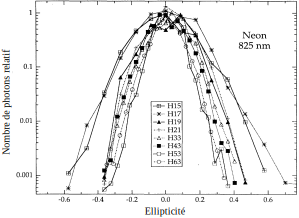
\includegraphics[width=0.6\columnwidth]{Figures/Polar/Intensity_f_ellipticity_budil}%
\caption{Intensité normalisée des harmoniques produites dans le néon en fonction de l'ellipticité. Tiré de \mycite{budilPRA1993}}%
\label{Fig:budil}%
\end{figure}

On observe une décroissance de l'intensité harmonique en fonction de l'ellipticité. Cet effet est marqué : on perd environ un ordre de grandeur en intensité quand $|\epsilon_{IR}| = 0.2$. On remarque également que cette décroissance est de plus en plus piquée lorsque l'ordre harmonique augmente.

\'{E}tudions ensuite les résultats de \mycite{AntoinePRA1997}. Les auteurs se sont cette fois intéressés à l'état de polarisation du rayonnement harmonique en fonction de l'ellipticité de l'infrarouge. Ces expériences ont été réalisées sur une version antérieure du système laser que nous avons utilisé dans la partie III. Pour caractériser le rayonnement, les auteurs mesurent des \textit{lois de Malus}, méthode optique qui sera présentée plus loin (section \ref{sec:resonant_argon_exp}). Comme on le verra, cette technique est incapable de mesurer le degré de polarisation $P$. Elle ne donne qu'une borne supérieure sur l'ellipticité, atteinte uniquement lorsque la lumière est complètement polarisée. Ce point est crucial dans le cas de la GHOE : comme expliqué dans la partie \ref{sec:introHHG}, le dipôle de chaque ordre harmonique dépend de l'intensité infrarouge. Le champ émis sera donc non homogène en polarisation spatialement et temporellement, donc nécessairement partiellement polarisé.

La figure \ref{fig:antoinepra} présente quelques résultats extraits de \mycite{AntoinePRA1997}. On y voit l'évolution de l'ellipticité des harmoniques et de l'angle d'orientation de l'ellipse $\eta$, pris par rapport à un axe de référence fixe. L'ellipticité mesurée n'étant qu'une borne supérieure de l'ellipticité vraie, on la note $\epsilon^{max}_q$. La figure \ref{fig:antoinepra} inclut un résultat numérique qui donne lui accès à $P$ et donne une idée de la quantité de lumière non-polarisée.

\begin{figure}[!ht]
\centering
\def\svgwidth{\columnwidth}
\import{Figures/Polar/}{antoinePRA.pdf_tex}
\caption{\`{A} gauche, mesure de l'ellipticité des harmoniques 17 et 23 générées dans l'argon par un champ infrarouge elliptique. Carrés rouges : mesures expérimentales de $\epsilon^{max}_q$ par loi de Malus. Comme expliqué plus haut, ce n'est qu'une borne supérieure sur la vraie valeur de l'ellipticité. En traits rouges, même quantité obtenue par le calcul. En pointillés noirs, véritable ellipticité obtenue par le calcul. En traits-pointillés verts, degré de polarisation obtenu par le calcul. \`{A} droite, mesure de l'angle de rotation de l'ellipse (carrés rouges) et même quantité obtenue par le calcul (traits rouges). Adapté de \mycite{AntoinePRA1997}.}
\label{fig:antoinepra}
\end{figure}

On fait les observations suivantes :
\begin{itemize}
\renewcommand{\labelitemi}{$\bullet$}
\setlength\itemsep{1em}
\item $\epsilon^{max}_q$ est une fonction croissante de $\epsilon_{IR}$ sur l'intervalle parcouru.
\item $|\epsilon^{max}_q|$ augmente plus rapidement avec $|\epsilon_{IR}|$ pour l'harmonique plus basse.
\item Le rayonnement est de moins en moins polarisé à mesure que $|\epsilon_{IR}|$ augmente. Cet effet est plus fort pour l'harmonique basse.
\item Cette diminution de $P$ s'accompagne d'une ellipticité vraie plus faible. Pour l'harmonique la plus basse, l'ellipticité vraie est presque \textit{deux fois inférieure} à l'ellipticité mesurée.
\item $\eta$ est également une fonction croissante de $\epsilon_{IR}$.
\item $\eta$ augmente plus rapidement pour l'harmonique basse.
\end{itemize}
\vspace{\baselineskip}
Ces deux travaux démontrent deux résultats généraux. En premier lieu, on voit que l'ellipticité de l'infrarouge est bien transférée au champ harmonique. Toutefois, l'ellipticité harmonique semble toujours rester inférieure à celle du laser générateur. Deuxièmement, le rendement harmonique décroît exponentiellement avec l'ellipticité de l'infrarouge. Nous concluons donc qu'il est très difficile d'obtenir un rayonnement ultraviolet d'ellipticité significative tout en gardant un niveau de signal suffisant. Dans la section suivante, nous expliquons les effets physiques à l'origine de ces propriétés.

\subsection{Description théorique de la GHOE en polarisation elliptique}
Dans le modèle à trois étapes (voir section \ref{sec:threestep}), la polarisation du champ intervient dans le calcul de la trajectoire électronique dans le continuum. On note $(x,y)$ la position dans le plan transverse de l'électron, que l'on considère classiquement. Sa trajectoire dans un champ complètement polarisé est donnée par :
\[\left\{
\begin{array}{l}
  \ddot{x}(t) = -\frac{qE_0}{m}\cos\omega t \\
  \ddot{y}(t) = -\epsilon\frac{qE_0}{m}\sin\omega t,
\end{array}
\right.\]
avec $q$ et $m$ la charge et la masse de l'électron, et $\epsilon$ et $\omega$ l'ellipticité et la fréquence angulaire du champ. L'équation selon $x$ se résoud exactement de la même façon que pour une polarisation linéaire : on suppose $x(t_i) = \dot{x}(t_i) = 0$, où $t_i$ est le temps d'ionisation, et pour chaque $t_i$, on obtient l'instant de recombinaison $t_r$.

Selon la dimension $y$, l'électron doit bien sûr être émis au niveau du noyau : $y(t_i) = 0$. Cependant, si on suppose que $\dot{y}(t_i) = 0$, l'équation $y(t_r) = 0$ n'a pas de solution : l'électron 'rate' l'atome et ne peut pas recombiner, comme illustré sur la figure \ref{fig:ellgruson}.

\begin{figure}[!ht]
\centering
\def\svgwidth{0.7\columnwidth}
\import{Figures/Polar/}{trajClassique.pdf_tex}
\caption{Trajectoire classique d'un électron dans un champ électrique elliptique, en supposant $x(t_i) = \dot{x}(t_i) = 0$ et $y(t_i) = \dot{y}(t_i) = 0$. La longueur d'onde est 800 nm et l'éclairement est $\SI{2e14}{W/cm^2}$. La polarisation du champ infrarouge est schématisée en gris. Adapté de \mycite{gruson}.}
\label{fig:ellgruson}
\end{figure}

Classiquement, la génération d'harmonique en polarisation elliptique est donc impossible. En vérité, le déplacement et la vitesse de l'électron selon l'axe $y$ sont trop faibles pour utiliser une description classique. Si on décrit cette dimension quantiquement, on a un paquet d'onde électronique émis lors de l'ionisation tunnel. Ce paquet d'onde est localisé spatialement autour de l'atome, sur une longueur $\Delta y$ dépendant de l'orbitale en jeu. Le moment cinétique selon $y$ est donc lui aussi confiné à une largeur $\Delta p_y$. La distribution de $p_y$ est centrée sur y=0 à $t=0$ et peut maintenant contenir des valeurs non nulles. \mycite{strelkov2006} démontre que pour avoir recombinaison, le moment cinétique initial doit valoir $p_y(t=0) = -\bar{y}/\tau$, où $\bar{y}$ est la quantité représentée sur la figure \ref{fig:ellgruson}, et $\tau$ le temps d'excursion total de l'électron. Ceci permet d'expliquer simplement le résultat de \mycite{budilPRA1993} présenté plus haut : si $\epsilon_{IR}$ augmente, $\bar{y}$ augmente également. Il faut donc un moment cinétique initial plus important pour avoir recombinaison, ce qui est moins probable puisque la distribution de $p_y(t=0)$ est centrée en y=0. Ceci explique la diminution du rendement harmonique avec l'ellipticité de l'infrarouge.

Pour comprendre qualitativement les résultats de \mycite{AntoinePRA1997}, on trace les trajectoires classiques de l'électron, cette fois avec la condition initiale $p_y(t=0) = -\bar{y}/\tau$ et avec les deux trajectoires quantiques.

\begin{figure}[!ht]
\centering
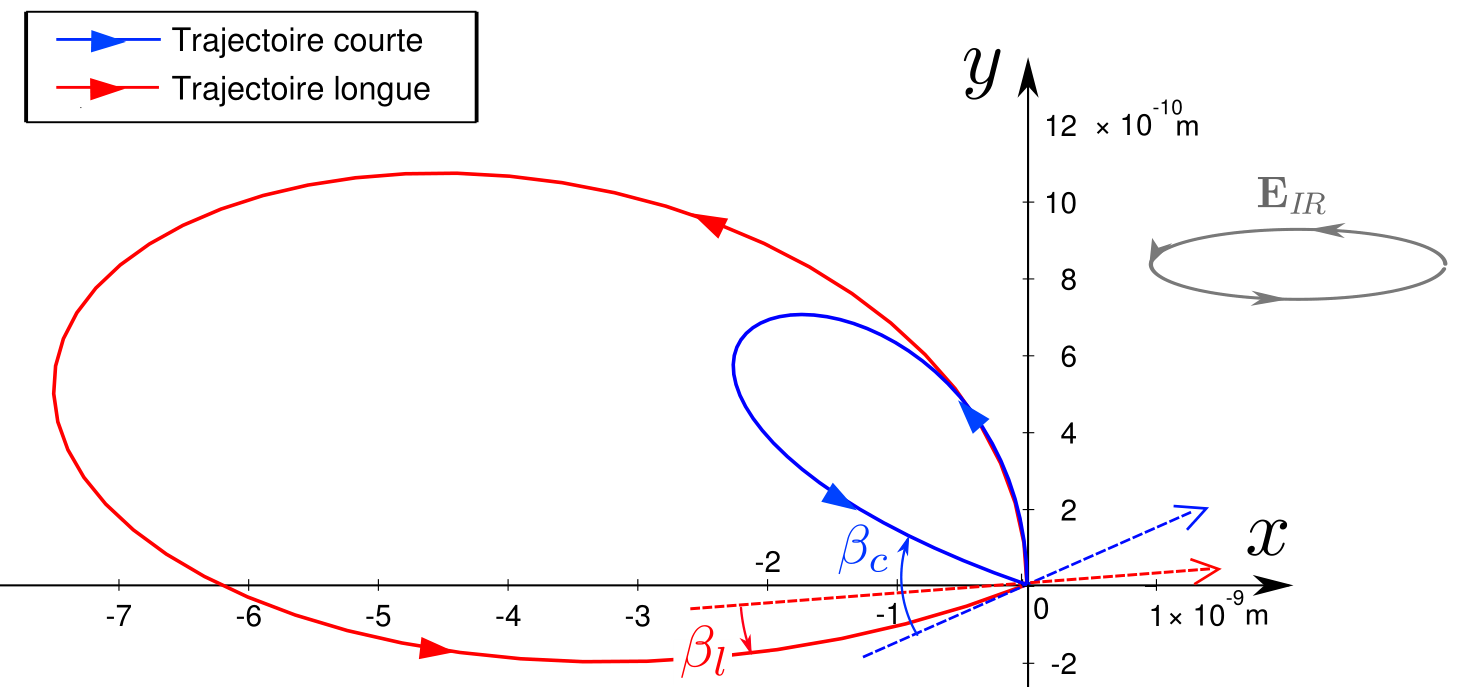
\includegraphics[width=0.9\columnwidth]{Figures/Polar/higuet.png}%
\caption{Trajectoires électroniques correspondant à l’harmonique 111 d'un laser à 1800 nm, pour un éclairement de $\SI{1e14}{W/cm^2}$ et une ellipticité de 0.2 (champ représenté en gris).
En ligne pointillée, la direction du champ à l’instant d’ionisation. On notera la différence entre les échelles
des axes $x$ et $y$. Tiré de \mycite{higuet}}
\label{fig:ellhiguet}%
\end{figure}

La figure \ref{fig:ellhiguet}, tirée de \mycite{higuet}, n'est pas directement comparable à la figure \ref{fig:ellgruson}, le calcul ayant été réalisé à une longueur d'onde plus élevée. Une longueur d'onde plus grande conduit à des trajectoires électroniques plus longues et à des effets plus marqués qu'à 800 nm.
On observe toutefois un effet intéressant : l'électron recombine sur l'atome avec un angle variable $\beta_{c/l}$ (pour trajectoire courte/longue). Cette angle est responsable de la rotation d'angle $\eta$ de l'ellipse harmonique. En effet, pour une orbitale de symétrie sphérique, l'axe principal de l'ellipse de polarisation du rayonnement harmonique est dirigé selon la direction de recollision de l'électron à la recombinaison \mycite{strelkov2006}. L'ellipse harmonique est donc tournée d'un angle $\beta_{c/l}\approx\eta$, qui dépend de l'ordre harmonique et de la trajectoire considérée. On remarque que $\beta_c$ et $\beta_l$ sont de signes différents, la dépendance de $\eta$ est donc de signe opposé pour la trajectoire longue. Ceci peut être mesuré expérimentalement (voir e.g. la figure 3.11 de \mycite{higuet}).\par
Enfin, cet angle explique également que le rayonnement harmonique soit elliptique. L'argument donné par \mycite{Strelkov2011} est le suivant : on considère un état lié $\psi_0(x,y,z) = \psi(x)\psi(y)\psi(z)$ et un paquet d'onde électronique. Ce paquet se déplace principalement dans la direction $x$ et possède une amplitude dans les deux autres dimensions : $\chi(x,y,z) = f(y,z)\exp(\rmi p_x x)$. Comme on l'a vu, l'amplitude $f(y,z)$ est initialement centrée en $y=0$ puis se décale selon $y$ au cours de la propagation. \`{A} la recombinaison, on peut faire un développement de Taylor de $f$ : $f(y,z) = f_0 + f_1 y$, où $f_1$ est relié à l'angle de recombinaison. Le moment dipolaire du système vaut 
\[\bm{d} = \int{\psi_0^* \bm{r} \chi \rmd\bm{r}} + \text{c.c.}\]
On obtient donc ses composantes cartésiennes :
\[d_x \propto f_0 \text{  et  } d_y \propto \rmi f_1.\]
On excite donc un dipôle dans les deux directions transverses, et leurs oscillations sont décalées de $\pi/2$. Le signal émis est donc polarisé elliptiquement.

\section{Méthodes existantes de génération d'harmoniques elliptiques}
Dans la partie précédente, nous avons expliqué le mécanisme de GHOE en polarisation elliptique et vu que le processus ne permettait pas un transfert direct et efficace de l'ellipticité de l'infrarouge vers l'ultraviolet. Nous présentons ici trois méthodes existantes pour circonvenir à ce problème. 

\subsection{Réflexion sur des surfaces métalliques}
\label{sec:metalsurface}
L'idée est ici de générer des harmoniques polarisée linéairement puis d'utiliser un dispositif similaire à une lame quart d'onde. Dans ces gammes spectrales, il est impossible de réaliser une lame quart-d'onde conventionnelle, mais on peut obtenir le même effet à partir de plusieurs surfaces métalliques. \par
On appelle plan d'incidence le plan formé par le vecteur d'onde du champ incident et le vecteur normal à la surface. Il est alors courant d'appeler $p$ la composante du champ \textit{parallèle} à ce plan et $s$ la composante perpendiculaire (\textit{senkrecht} en allemand). Selon le métal utilisé, ces deux composantes ne sont pas réfléchies également : la surface métallique présente une réflectivité selon chaque dimension, habituellement notées $R_p$ et $R_s$. De plus, elle introduit un déphasage entre ces deux composantes. Il est ainsi possible d'introduire un déphasage de $\pi/2$ en choisissant une bonne combinaison de miroirs. \mycite{VodungboOE2011} ont développé un dispositif à 4 miroirs de Mo/$\text{B}_\text{4}$C qui permettent d'obtenir les harmoniques 31 à 45 avec une ellipticité variant de 1 à 0.61. Ces caractéristiques sont très intéressantes, malgré un inconvénient majeur : la transmission du dispositif varie entre 2.6 et 3.7 \% sur la plage considérée. Ce type de dispositif a continué à être amélioré, \mycite{WillemsPRB2015} reportent par exemple une transmission de 10-30\% et une ellipticité de $\approx 0.8$ entre 45 et 70 eV.\par

Ces dispositifs sont assez difficiles à implémenter, ce qui couplé à leur faible transmission explique qu'ils ne soient pas très répandus aujourd'hui. 

\subsection{Génération dans des molécules alignées}
Considérons la GHOE avec un faisceau polarisé linéairement, cette fois dans un gaz de molécules diatomiques. Au niveau microscopique, l'orientation de l'axe de la molécule par rapport à la polarisation du laser joue un rôle crucial : l'angle de recombinaison de l'électron par rapport à cet axe modifie l'émission, exactement comme le champ elliptique représenté sur la figure \ref{fig:ellhiguet}. L'électron peut donc exciter les deux composantes du dipôle. L'interprétation est toutefois plus compliquée, puisque l'ellipticité obtenue dépend de la symétrie de ou des orbitales ionisées, de leur phases relatives ou encore de l'intensité de génération (voir \mycite{MairessePRL2010}). \par
\`{A} l'échelle macroscopique, toutes les orientations de molécules par rapport au laser sont équiprobables. On a donc un effet de moyenne, qui donne un rayonnement harmonique macroscopique polarisé linéairement. Il faut donc \textit{aligner} les molécules. Une technique courante est l'alignement impulsionnel, qui utilise une pré-impulsion quelques secondes avant l'impulsion de génération \mycite{RoscaPRL2001}. La figure \ref{fig:n2ell} présente deux exemples de résultats obtenus avec $\text{N}_\text{2}$, tirés de \mycite{ZhouPRL2009} et \mycite{MairessePRL2010}. Dans les deux cas, on observe un maximum d'ellipticité pour l'harmonique 23 et pour un angle d'alignement d'environ 60\degres.

\begin{figure}[!ht]
\centering
\def\svgwidth{1\columnwidth}
\import{Figures/Polar/}{n2ell.pdf_tex}
\caption{Mesures d'ellipticité en fonction de l'ordre harmonique et de l'angle d'alignement des molécules de $\text{N}_\text{2}$ par rapport à la polarisation du laser. \`{A} gauche, résultat tiré de \mycite{ZhouPRL2009}, où I = $\SI{2e14}{W/cm^2}$. \`{A} droite, résultat tiré de \mycite{MairessePRL2010}, où I = $\SI{8e13}{W/cm^2}$. Les ellipticités mesurées ici sont des bornes supérieures et non pas la vraie valeur.}
\label{fig:n2ell}
\end{figure}

Ce résultat s'explique en fait par la présence de plusieurs canaux d'ionisation et est donc très intéressant du point de vue de la spectroscopie harmonique. Il est toutefois assez peu flexible et nécessite d'aligner des molécules, et fournit une ellipticité modeste. De plus, l'utilisation d'une impulsion d'alignement a tendance à créer davantage d'inhomogénéités spatiales et temporelles, ce qui produit un rayonnement peu polarisé. Cette question est étudiée en détail expérimentalement dans la thèse de Vincent Gruson \mycite{gruson}.

\subsection{Manipulation de la trajectoire électronique par un champ bicolore}
Terminons par la méthode la plus récente, qui est peut-être la plus intuitive. Le principe est ici de contrôler optiquement la trajectoire électronique de sorte à ce que la recombinaison soit possible quelque soit l'ellipticité infrarouge. Une solution à ce problème a été initialement donnée par \mycite{EichmannPRA1995}. En utilisant un champ à deux couleurs d’ellipticités opposées et de deux longueurs d'onde commensurables, par exemple 400 et 800 nm, la GHOE est possible. L'expérience réalisée par \mycite{FleischerNP2014} montre que la génération est efficace dans ces conditions, et permet de générer des harmoniques paires et impaires d'ellipticité $|\epsilon^{max}_q|\approx 1$. \mycite{KfirNP2015} a mesuré l'hélicité (le signe de $\epsilon$) et montré que les ordres harmoniques étaient polarisés ainsi:
\[\left\{
\begin{aligned}
  \text{Si }q&=3m-1,\quad &\epsilon_q \approx \pm 1 \\
	&=3m+1, &\epsilon_q \approx \mp 1 \\
	&=3m, &\text{l'harmonique n'est pas générée},
\end{aligned}
\right.\]
où $\pm$ dépend de l'hélicité des champs générateurs. Cette méthode est très intéressante car elle produit un rayonnement fortement polarisé et intense. Elle a été utilisée avec succès par \mycite{KfirNP2015} pour réaliser des mesures de dichroïsme circulaire magnétique dans le cobalt, un effet voisin de ceux dont il sera question au chapitre \ref{sec:PECD}. Cette méthode est ainsi particulièrement adaptée à la spectroscopie de la phase solide.\par
La réponse d'une molécule est quant à elle plus difficile à interpréter. En effet, un grand nombre de degrés de liberté et différents canaux d'ionisation contribuent au spectre total, et il n'est jamais facile d'identifier chacune de ces contributions. 
On préférera donc avoir un rayonnement très simple, de sorte à exciter le moins d'effets possibles et de pouvoir les identifier. La technique présentée ici fournit un spectre harmonique dense fait d'harmoniques paires et impaires d'hélicité en alternance, ce qui est à l'opposé des besoins de la spectroscopie moléculaire.

\section{Une image photonique de la GHOE en polarisation elliptique}
Les travaux de \mycite{FleischerNP2014} que nous venons de mentionner ont suscité de nombreuses questions sur la conservation du moment angulaire de spin dans la GHOE. Avant ces travaux, la conservation du spin n'avait été étudiée ni théoriquement, ni expérimentalement.

Jusqu'à présent, nous avons utilisé une description macroscopique du champ électromagnétique. \`A l'étape de recombinaison de la GHOE, l'électron recombine sur l'état fondamental de l'atome. Le processus de GHOE peut être vu comme un processus \textit{paramétrique} dans lequel l'état initial et final sont les mêmes. On considère alors que chaque photon harmonique est issu de l'absorption et/ou de l'émission d'un certain nombre de photons du fondamental. Si la GHOE est effectivement un processus paramétrique, elle doit conserver l'énergie, la quantité de mouvement et les moments angulaires orbitaux et de spin. Nous avons pu observer la conservation des trois premières quantités au cours de cette thèse, et nous intéressons ici à la quatrième.

\mycite{FleischerNP2014} ont proposé un modèle simple prédisant le MAS de chaque harmonique dans leur dispositif à deux couleurs, en supposant la conservation du MAS. De manière surprenante, ils observèrent de très larges déviations à ce modèle et proposèrent deux mécanismes pour les expliquer : (1) l'électron ionisé emporte avec lui un moment angulaire de spin non nul, ce qui remet en question le fait que la GHOE soit un processus paramétrique, et (2) les différentes harmoniques sont émises de façon corrélées, ce qui empêche de considérer le moment angulaire de spin d'une harmonique seule.\par
\mycite{PisantyPRA2014} proposa ensuite un modèle différent, qui montra que les données de \mycite{FleischerNP2014} étaient cohérentes avec la conservation du MAS sans avoir à utiliser de tels arguments. Nous reprenons sa démarche pour expliquer le cas plus simple de la génération à un seul faisceau polarisé elliptiquement, déjà décrit macroscopiquement dans la partie \ref{sec:ghoepolar}, mais cette fois avec une image photonique.

On considère un champ d'ellipticité $\epsilon_0$ arbitraire. On décompose ce champ sur la base des ondes circulaires droites et gauches :
\begin{equation}
\bm{E} = \frac{E_0 e^{-\rmi\omega t}}{2\sqrt{2}}\left(\frac{1+\epsilon_0}{\sqrt{1+\epsilon_0^2}}\bm{e}_R+\frac{1-\epsilon_0}{\sqrt{1+\epsilon_0^2}}\bm{e}_L\right)+\text{c.c.},
\label{eq:Eell_RL}
\end{equation}
où $\bm{e}_{R/L}=(\bm{e}_x\pm\rmi\bm{e}_y)/\sqrt{2}$ sont les vecteurs unitaires complexes des polarisations circulaires droites et gauches.

Les composantes R et L du champ sont alors considérées séparément : on note $n_R$ et $n_L$ le nombre de photons respectif impliqués dans le processus. On note $q$ l'ordre harmonique, et la conservation de l'énergie s'écrit :
\[ q\hbar\omega = n_R\hbar\omega+n_L\hbar\omega, \]
soit $q = n_R + n_L$, ce qui est consistant avec la conservation de la parité car le nombre de photon absorbé est impair. On a donc un grand nombre de paires $(n_R,n_L)$ qui contribuent à l'émission de chaque harmonique $q$. On peut restreindre ces paires en écrivant la conservation du moment angulaire de spin pour chacune d'entre elles. En notant $s$ le MAS, on a :
\[s_{(n_R,n_L)} = n_R s_R + n_L s_L = n_R - n_L.\]
Le MAS d'un photon ne peut prendre que deux valeurs : $s_{(n_R,n_L)}=\pm1$, ce qui restreint les canaux possibles à 2 :
\[n_R = \frac{q+1}{2},\; n_L = \frac{q-1}{2}\quad\text{ou}\quad n_R = \frac{q-1}{2},\; n_L = \frac{q+1}{2}.\]

Ces deux canaux n'ont pas la même amplitude. Par simplicité, on suppose que l'amplitude d'un processus à n-photons évolue comme la $\text{n}^{i\`{e}me}$ puissance du champ fondamental. Cette approximation est un développement perturbatif à l'ordre le plus bas, qui a de nombreuses limitations pour la description de la GHOE, comme l'absence de plateau. On verra qu'elle permet toutefois de comprendre les comportements observés. Dans cette approximation, l'expression \ref{eq:Eell_RL} donne l'amplitude de chaque canal :
\[ E_{(n_R,n_L)} \propto \left(\frac{1+\epsilon_0}{\sqrt{1+\epsilon_0^2}}\right)^{n_R}\left(\frac{1-\epsilon_0}{\sqrt{1+\epsilon_0^2}}\right)^{n_L}\]
donc son intensité est :
\[ I_{(n_R,n_L)} \propto \left(\frac{1+\epsilon_0}{\sqrt{1+\epsilon_0^2}}\right)^{2n_R}\left(\frac{1-\epsilon_0}{\sqrt{1+\epsilon_0^2}}\right)^{2n_L}\]

On somme alors les deux canaux pondérés par $I_{(n_R,n_L)}$ pour obtenir la valeur moyenne du MAS de chaque harmonique :
\begin{align}
<s_q> &= \frac{I_{(\frac{q+1}{2},\frac{q-1}{2})} s_{(\frac{q+1}{2},\frac{q-1}{2})}+I_{(\frac{q-1}{2},\frac{q+1}{2})} s_{(\frac{q-1}{2},\frac{q+1}{2})}}{I_{(\frac{q+1}{2},\frac{q-1}{2})}+I_{(\frac{q-1}{2},\frac{q+1}{2})}}\nonumber\\
&= \frac{\left(\frac{1+\epsilon_0}{\sqrt{1+\epsilon_0^2}}\right)^{q+1}\left(\frac{1-\epsilon_0}{\sqrt{1+\epsilon_0^2}}\right)^{q-1}
-
\left(\frac{1+\epsilon_0}{\sqrt{1+\epsilon_0^2}}\right)^{q-1}\left(\frac{1-\epsilon_0}{\sqrt{1+\epsilon_0^2}}\right)^{q+1}
}{
\left(\frac{1+\epsilon_0}{\sqrt{1+\epsilon_0^2}}\right)^{q+1}\left(\frac{1-\epsilon_0}{\sqrt{1+\epsilon_0^2}}\right)^{q-1}
+
\left(\frac{1+\epsilon_0}{\sqrt{1+\epsilon_0^2}}\right)^{q-1}\left(\frac{1-\epsilon_0}{\sqrt{1+\epsilon_0^2}}\right)^{q+1}
}\nonumber\\
&= \frac{2\epsilon_0}{1+\epsilon_0^2}
\label{eq:mas_q}
\end{align}

On obtient également l'évolution de l'intensité harmonique en fonction de l'ellipticité comme la somme de l'intensité des deux canaux :
\begin{align}
I_q &= \frac{1}{2}\left[\left(\frac{1+\epsilon_0}{\sqrt{1+\epsilon_0^2}}\right)^{q+1}\left(\frac{1-\epsilon_0}{\sqrt{1+\epsilon_0^2}}\right)^{q-1}+\left(\frac{1+\epsilon_0}{\sqrt{1+\epsilon_0^2}}\right)^{q-1}\left(\frac{1-\epsilon_0}{\sqrt{1+\epsilon_0^2}}\right)^{q+1}\right]\nonumber\\
&= \left(\frac{(1+\epsilon_0)(1-\epsilon_0)}{\sqrt{1+\epsilon_0^2}}\right)^{q}\times\frac{1+\epsilon_0^2}{1-\epsilon_0^2}
\label{eq:I_q}
\end{align}

Ces deux quantités sont tracées sur la figure \ref{fig:mas_photon}. Ce modèle simple reproduit qualitativement les mesures de \mycite{AntoinePRA1997} et \mycite{budilPRA1993} (figures \ref{fig:antoinepra} et \ref{Fig:budil}) : l'ellipticité harmonique augmente avec l'ellipticité du fondamental, et l'efficacité du processus décroît exponentiellement. On retrouve également la décroissance de l'efficacité plus rapide pour les ordres plus élevés, due à au terme en puissance de $q$ dans l'équation \ref{eq:I_q}. Ce modèle ne décrit par contre pas l'évolution du MAS entre différents ordres harmoniques, l'équation \ref{eq:mas_q} ne dépendant pas de $q$.

\begin{figure}[!ht]
\centering
\def\svgwidth{1\columnwidth}
\import{Figures/Ell_Photon/}{I_photon.pdf_tex}
\caption{\'Evolution de l'intensité et du moment angulaire de spin harmonique en fonction de l'ellipticité du fondamental. Résultat d'un modèle perturbatif simple.}
\label{fig:mas_photon}
\end{figure}

\chapter{Harmoniques elliptiques produites par GHOE résonante}
Nous présentons ici notre méthode pour produire un rayonnement ultraviolet polarisé elliptiquement. Cette source a été développée pour l'étude de la photoionisation de molécules. Ces travaux, ainsi que la totalité du reste de ce chapitre, ont été réalisés au CELIA Bordeaux en collaboration avec l'équipe de Yann Mairesse. Les résultats correspondant aux parties \ref{sec:sf6ghoe} à \ref{sec:results_fenchone} ont été publiés dans \mycite{FerreNP2015}, Article \ref{pap:FerreNP2015} inclus dans cette thèse.

L'idée ici est de modifier la dynamique électronique dans la GHOE non pas en structurant le champ laser, mais en utilisant le potentiel de la molécule lui-même. En particulier, ce potentiel peut être structuré par la présence de \textit{résonances}. Ces phénomènes ont été très largement étudiés dans le cadre de la photoionisation, et se manifestent en général par une augmentation de la section efficace d'absorption pour une énergie de photon précise. Cette énergie résonante coïncide avec l'énergie nécessaire à un des canaux d'ionisation de la molécule, ce qui ouvre ce canal et augmente la section efficace. Cette augmentation dépend de la force d'oscillateur de cette transition. De nombreux mécanismes sont connus et documentés par des études réalisées sur synchrotron, peuvent impliquer un ou plusieurs électrons, ou encore apparaître en dessous ou au dessus du seuil d'ionisation.

La photoionisation est le processus conjugué à la recombinaison radiative. Il est donc naturel que des effets des résonances moléculaires soient visibles en GHOE, où la recombinaison joue un rôle central. Une résonance peut avoir des effets très variés sur la GHOE. L'étape résonante peut être soit l'ionisation, par exemple dans le cas d'une résonance multiphotonique \mycite{AckermannOE2012,ChuPRA2013}, soit à la recombinaison, qui peut être magnifiée par une résonance de forme ou par un piégeage dans un état de Rydberg \mycite{TaeibPRA2003,TudorovskayaPRA2011}. La présence d'une résonance empêche souvent de réaliser l'approximation de champ fort et met en défaut le modèle à trois étapes \mycite{StrelkovPRL2010}. Commençons par étudier le cas de l'argon.

\section{Génération résonante dans l'argon : cas des résonances sous le seuil}
\subsection{Mécanismes résonants autour du seuil}
La figure \ref{fig:ArIp} montre la section efficace de photoabsorption de l'argon. On y voit une série de pics d'absorption en dessous du seuil d'ionisation, qui correspondent aux états de Rydberg de l'atome.

\begin{figure}[!ht]
\centering
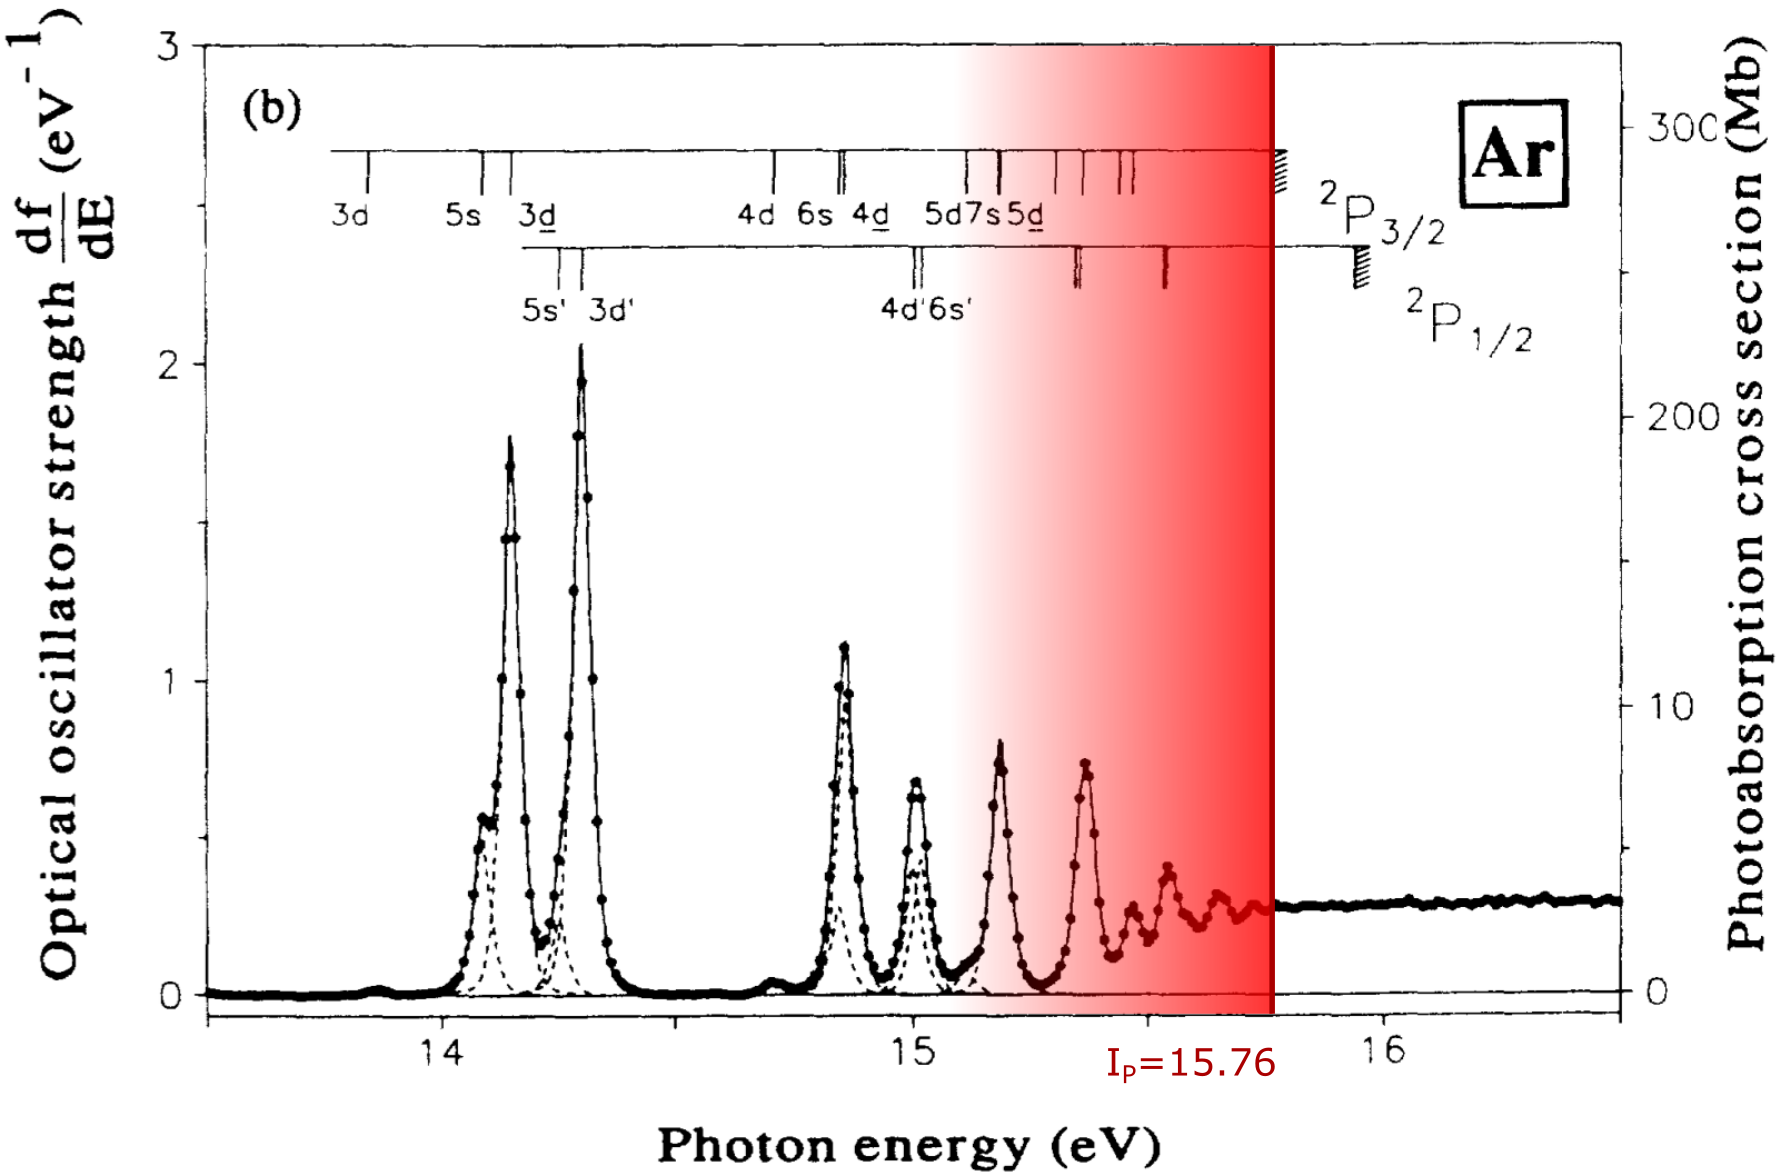
\includegraphics[width=0.9\columnwidth]{Figures/ResonantArgon/argon_spectrum.png}%
\caption{Section efficace de photoabsorption de l'argon dans la gamme 13.5-16.5 eV. Les lignes pointillées correspondent aux pics déconvolués. Tiré de \mycite{ChanPRA1992}.}
\label{fig:ArIp}%
\end{figure}

Nous allons voir que cette structure bien particulière donne lieu à plusieurs phénomènes intéressants. L'argon est un système de choix car son potentiel d'ionisation ($I_p = \SI{15.76}{eV}$) est très proche de l'énergie de 10 photons d'un laser Ti:Sa ($10\times 1.55 = 15.5$ eV). L'étude de la GHOE au voisinage du potentiel d'ionisation a été réalisée expérimentalement par \mycite{ChiniNP2014}, qui observèrent une émission à la fois en dessous et au dessus du seuil. Cette émission semble avoir des caractéristiques inhabituelles par rapport à la GHOE classique. En particulier, les auteurs remarquent une augmentation du signal avec la pression sans observer de phénomène de saturation, mais n'expliquent pas le mécanisme sous-jacent. Ensuite, \mycite{XiongPRL2014} et surtout \mycite{CampPRA2015} expliquent ce mécanisme en détail et montrent qu'il est lié à la présence des états de Rydberg de la figure \ref{fig:ArIp}. Deux effets distincts interviennent dans la génération.

Le premier est un mécanisme de GHOE résonante ayant lieu pendant l'ionisation de l'atome. Pendant la durée du pulse, tous les niveaux énergétiques de l'atome sont décalés par effet Stark. Pour les états de Rydberg de la figure \ref{fig:ArIp}, ce décalage vaut environ $U_p$, l'énergie pondéromotrice \mycite{GaardePRA2001,FiguieraPRA2002}. Ainsi, l'énergie d'un de ces niveaux peut devenir égale à l'énergie de $n$ photons infrarouges (dans notre cas, $n=10$). On a alors une résonance multi-photonique, qui augmente drastiquement l'intensité de la $n$-ième harmonique. La condition de résonance s'écrit : $n\hbar\omega = |E_R-E_0|+U_p$, où $E_R$ et $E_0$ sont respectivement les énergies de l'état fondamental et de l'état de Rydberg. Ce phénomène était déjà connu en ionisation au-dessus du seuil (ATI pour \textit{Above Threshold Ionization}) avec des impulsions courtes \mycite{FreemanPRL1987,AgostiniPRL1989}. On remarquera que pour l'argon, l'ordre harmonique résonant est le 10ème, qui n'est pas généré dans les conditions habituelles. Pour observer cet effet, on utilisera donc soit des impulsions infrarouges très courtes, soit on choisira une autre longueur d'onde de génération. Dans la suite, nous utiliserons une longueur d'onde de 400 nm, pour laquelle on a une résonance à 5 photons au seuil de l'argon.

Le second effet ne correspond pas à la GHOE, mais produit quand même un rayonnement ultraviolet dans cette région. Dans ce mécanisme, le faisceau infrarouge crée une superposition d'état cohérente entre l'état fondamental d'énergie $E_0$ et quelques états de Rydberg d'énergie $E_R$, via une transition multiphotonique. Le dipôle ainsi créé émet une radiation d'énergie $E_R-E_0$ pendant une durée correspond à la durée de vie de l'état de Rydberg, c'est-à-dire bien plus longtemps que l'émission harmonique. Ce rayonnement a donc une structure spectrale très fine. Ce processus s'appelle \textit{Free Induction Decay} ultraviolet (xFID) \mycite{BengtssonLarsenEtAl2015}, et était déjà connu en Résonance Magnétique Nucléaire \mycite{BlockPR1946} et dans l'infrarouge \mycite{BrewerPRA1972}. 

L'influence de ces deux effets a été étudiée expérimentalement en détail au CELIA Bordeaux par \mycite{beaulieuArXiv2016}. Des expériences réalisées à 800 nm ont permis d'observer les rayonnements issus de chacun de ces deux effets et d'étudier leurs propriétés de cohérence temporelle. Un spectre typique obtenu avec une impulsion de 7 fs est présenté sur la figure \ref{fig:xFID}. Les auteurs démontrent également la possibilité d'avoir ionisation à partir d'un état de Rydberg excité et recombinaison sur l'état fondamental, ce qui donne l'émission pointée par la ligne violette sur la figure \ref{fig:xFID}. 

\begin{figure}[!ht]
\centering
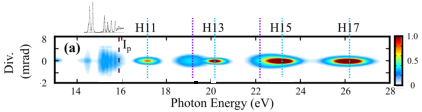
\includegraphics[width=1.1\columnwidth]{Figures/ResonantArgon/xFID.pdf}%
\caption{Spectre obtenu dans l'argon avec une impulsion de 7 fs à 800 nm. L'intensité est de $\SI{5.2e13}{W/cm^2}$. On observe le rayonnement xFID en dessous du seuil d'ionisation, que l'on compare avec le spectre d'absorption tiré de la figure \ref{fig:ArIp}. Ensuite, on observe les harmoniques non résonantes (lignes verticales bleues) ainsi que celles provenant d'états de Rydberg excités (lignes verticales violettes). Tiré de \mycite{beaulieuArXiv2016}.}
\label{fig:xFID}
\end{figure}

L'effet xFID est également très intéressant fondamentalement et permet de mesurer des observables similaires à celles obtenue en spectroscopie d'absorption transitoire attoseconde (ATAS, pour \textit{Attosecond Transient Absorption Spectroscopy}) \mycite{BeckNJP2014}. En collaboration avec Samuel Beaulieu, \'{E}tienne Bloch, Valérie Blanchet et Yann Mairesse, nous avons étudié ce point expérimentalement, cette fois avec une longueur d'onde de 400 nm et en choisissant des conditions de focalisation favorisant grandement le xFID. Ces expériences sont en cours d'analyse et ne seront pas présentées dans ce manuscrit. Nous nous intéressons maintenant à la polarisation du rayonnement au voisinage du seuil d'ionisation.

\subsection{Ellipticité du rayonnement près du seuil de l'argon}
\label{sec:resonant_argon_exp}
Pour avoir une résonance multiphonique au seuil de l'argon, nous choisissons de travailler à 400 nm. L'utilisation de cette longueur d'onde a deux autres avantages : (1) La GHOE est plus efficace, l'efficacité évolue en effet en $\lambda^{\simeq-6}$ \mycite{ShinerPRL2009}. (2) La largeur spectrale entre chaque harmonique est doublée et l'énergie de coupure diminue, on aura donc très peu d'harmoniques. Comme on le verra, ceci est très favorable dans les expériences de dichroïsme circulaire présentées plus loin. 

Ces expériences et toutes celles qui vont suivre ont été réalisées sur le système Aurore du CELIA Bordeaux, qui délivre des impulsions de 8mJ, 25 fs à environ 800 nm et à un taux de répétition de 1 kHz. Ce faisceau est ensuite doublé en fréquence par un BBO de type 1 et de $\SI{200}{\micro\meter}$ d'épaisseur. On mesure qu'à partir de 4 mJ du fondamental, on obtient 1 mJ à 404 nm. Le 800 nm restant est filtré à l'aide de miroir dichroïques, tandis que le 400 nm est focalisé par une lentille mince de Si$\text{O}_\text{2}$ de 50 cm de focale. Le reste du dispositif est similaire à celui présenté sur la figure \ref{Fig:ExpG} : des harmoniques sont générées dans un jet de gaz continu (ouverture de $\SI{300}{\micro\meter}$) puis imagées par un réseau de diffraction couplé à une galette de micro-canaux. 

Dans ce dispositif de GHOE assez typique, nous souhaitons rajouter une mesure de l'état de polarisation du rayonnement. Nous choisissons de mesurer des \textit{loi de Malus}. Habituellement, ces lois sont obtenues en mesurant l'intensité transmise par un polariseur parfait en fonction de l'angle du polariseur $\theta_p$ par rapport au champ électrique. Si le champ électrique est polarisé linéairement, l'intensité sera totalement transmise lorsque le polariseur est orienté parallèlement à la direction de polarisation du champ, et non transmise s'il est orthogonal. A contrario, si le champ est circulaire, l'intensité transmise ne variera pas en fonction de $\theta_p$. De manière générale, on obtient un signal oscillant de la forme 
\[I(\theta_p) = \epsilon^2+(1-\epsilon^2)\cos^2(\eta-\theta_p),\]
où $\epsilon$ et $\eta$ ont été définis dans la partie \ref{sec:polardef}. Remarquons que ce type de mesure est insensible à la partie non polarisée de la lumière, dont la contribution ne dépend pas de $\theta_p$. Ainsi, la valeur d'$\epsilon$ mesurée ici est encore une fois uniquement une borne supérieure, $\epsilon^{max}$. On voit donc que seulement pour une onde totalement polarisée, la mesure d'une loi de Malus donne accès à tous les paramètres de Stokes, définis plus haut. 

Il reste donc à réaliser un polariseur pour le rayonnement harmonique. Nous avons déjà mentionné que les surfaces métalliques présentaient des réflexions $R_s$ et $R_p$ différentes selon chaque dimension transverse (voir section \ref{sec:metalsurface}). Ainsi, en utilisant plusieurs de ces surfaces à la suite, on peut quasiment filtrer la composante $s$ ou $p$. Nous choisissons d'utiliser trois miroirs avec revêtement en or placés à 75\degres-60\degres-75\degres, ce qui donne un rapport total $R_s/R_p$ valant 5 à 20 pour la gamme spectrale étudiée. Enfin, plutôt que de motoriser et de faire tourner ce polariseur sous vide, on préfère tourner l'orientation du champ de génération et garder le polariseur fixe, ce qui est équivalent. Ce polariseur imparfait doit être pris en compte dans l'analyse de la loi de Malus (voir \mycite{AntoinePRA1997} ainsi que \mycite{gruson}), mais n'empêche pas de mesurer les paramètres recherchés, comme l'illustre la figure \ref{fig:malus} pour l'harmonique 5. Pour plus de détail sur ce dispositif de polarimétrie harmonique on se reportera à la thèse d'Amélie Ferré \mycite{ferre}.

\begin{figure}[!ht]
\centering
\def\svgwidth{0.7\columnwidth}
\import{Figures/ResonantArgon/}{malus.pdf_tex}
\caption{Lois de Malus pour l'harmonique 5 du faisceau à 404 nm. On mesure l'intensité transmise par le polariseur XUV en fonction de la direction de polarisation du champ de génération, lorsqu'il est polarisé linéairement (rouge) ou elliptiquement (vert). On voit que le champ harmonique est maximal en $\theta_p = \eta$, ce qui donne la direction de son ellipse de polarisation. Par ailleurs, on observe une diminution du contraste des oscillations avec $\epsilon_{IR}$, signe d'une ellipticité harmonique plus élevée. L'analyse des oscillations donne ici $\epsilon_q^{max} \simeq 0.6$ quand $\epsilon_{IR}=0.287$.}
\label{fig:malus}
\end{figure}

La figure \ref{fig:resonant_argon_exp} présente les résultats obtenus lorsque le laser de génération porte une ellipticité $\epsilon_{IR} = 0.4$. On observe les harmoniques 5, 7 et 9 du fondamental à 404 nm. Les harmoniques 7 et 9 présentent un profil gaussien spectralement, tandis que l'harmonique 5 est structurée. Cette structure est due au xFID, effet présenté plus haut. Le rayonnement xFID est superposé à l'émission harmonique, qui est résonante due à la résonance à 5 photons.  On mesure ensuite l'ellipticité en fonction de l'énergie de photon. On voit que l'ellipticité apparente des harmoniques non résonantes est de l'ordre de $\epsilon_{IR}$, tandis que celle de l'harmonique résonante est presque doublée (valeur maximale de 0.77).  

\begin{figure}[!ht]
\centering
\def\svgwidth{1\columnwidth}
\import{Figures/ResonantArgon/}{exp_result.pdf_tex}
\caption{Mesure d'ellipticité dans l'argon près du seuil d'ionisation. Le laser à 404 nm a une ellipticité de $\epsilon_IR=0.4$. Sur l'échelle de gauche (bleue), intensité en fonction de l'énergie de photon. On observe trois harmoniques, desquelles on mesure l'ellipticité apparente. On obtient les courbes rouges, échelle de droite.}
\label{fig:resonant_argon_exp}
\end{figure}

Pour confirmer que cette forte ellipticité est due à la présence de résonances, Bernard Pons et Baptiste Fabre, du CELIA Bordeaux, ont réalisé une étude théorique du problème. On résout l'équation de Schrödinger dépendante du temps (TDSE, \textit{Time-Dependant Schrödinger Equation}) à deux dimensions, en utilisant un potentiel de Coulomb de "cœur mou", qui reproduit la présence du potentiel d'ionisation et des états sous-jacents. La figure \ref{fig:resonant_argon_th_bound} illustre ce potentiel ainsi que le spectre harmonique obtenu. On observe des structures spectrales similaires à l'expérience, à la fois dans l'intensité et dans l'ellipticité de l'harmonique 5. L'ellipticité est en particulier très modulée, mais ne prend pas des valeurs aussi élevées que celles mesurées. Au contraire, elle devient même négative à 14 eV. Les calculs ont été répétés et ont permis d'observer qu'une très légère modification du potentiel atomique donnaient lieu à de très fortes modifications de l'ellipticité. On s'attend donc à n'avoir qu'un accord qualitatif.

\begin{figure}[!ht]
\centering
\def\svgwidth{1\columnwidth}
\import{Figures/ResonantArgon/}{th_result_bound.pdf_tex}
\caption{Résultat théorique en utilisant un potentiel de Coulomb de cœur mou. En haut, on représente le profil de ce potentiel, qui peut être ajusté pour obtenir la bonne valeur d'$\text{I}_{\text{p}}$. En bas, mêmes grandeurs que celles mesurées expérimentalement sur la figure \ref{fig:resonant_argon_exp}.}
\label{fig:resonant_argon_th_bound}
\end{figure}

En conclusion, nous voyons que la présence de résonances sous le seuil induit une modulation de l'ellipticité. Nous mesurons de plus qu'elle augmente très fortement. On obtient donc un rayonnement aux propriétés intéressantes sans véritable perte de signal : une mesure par une photodiode calibrée montre que l'harmonique 5 contient $\num{7e6}$ photons par impulsion. De plus, le caractère résonant de l'harmonique 5 fait qu'elle ne subit pas d'effet de réabsorption \mycite{ChiniNP2014}. Son flux peut donc être facilement augmenté par une pression de génération plus élevée.  Toutefois, cette méthode est restreinte à des énergies de photons relativement basses, correspondant au seuil d'ionisation du gaz utilisé. Les gaz habituellement utilisés pour avoir un flux important sont l'argon, $\text{I}_{\text{p}}=15.76$ eV, le krypton, $\text{I}_{\text{p}}=14$ eV, ou le xénon, $\text{I}_{\text{p}}=12.13$ eV. Il serait donc intéressant de généraliser notre approche à d'autres résonances d'énergie plus élevée. Dans la section suivante, nous étudions le cas de résonances dans le continuum.

\section{Génération autour d'une résonance dans le continuum}
Ces résonances se manifestent de la même façon que celles présentées plus haut : une augmentation de la section efficace de photoionisation. Nous nous intéressons au cas des \textit{résonances de forme} \mycite{Dehmer1972}, couramment observées dans le spectre de petites molécules. Bien qu'elles aient été observées assez tôt, leur interprétation et leur définition fait régulièrement débat, comme en témoigne l'article de \mycite{Piancastelli1999}, intitulé "\textit{The neverending story of shape resonances}" . Une interprétation courante est la suivante. Ces résonances sont dues à une barrière présente dans le potentiel moléculaire. Cette barrière est la résultante de forces attractives (e.g. coulombienne) et répulsives (effets d'écrantage, force centrifuge). Quand un photoélectron possède l'énergie correspond à cette barrière, il se retrouve dans un état métastable \mycite{simons1984roles}, piégé dans la barrière de potentiel, dont il finit par s'échapper par effet tunnel. La figure \ref{fig:shaperesonance} illustre ce principe : à l'énergie résonante, la fonction d'onde électronique est localisée sur le puit central et temporairement piégée.

\begin{figure}[!ht]
\centering
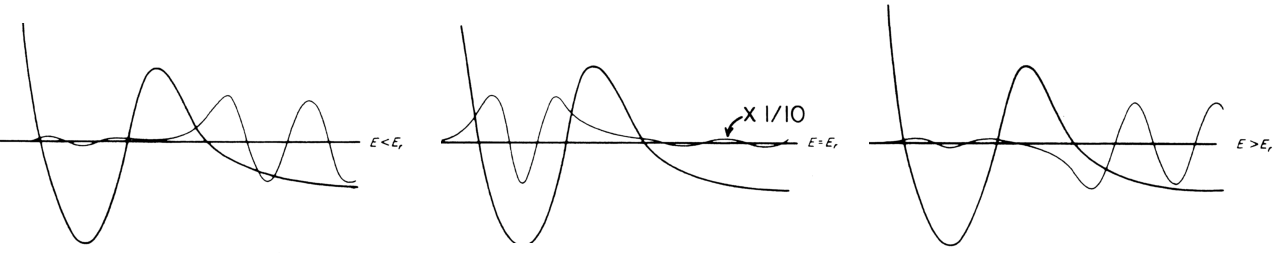
\includegraphics[width=1\columnwidth]{Figures/ResonantArgon/shape_resonance.pdf}%
\caption{Principe d'une résonance de forme. De gauche à droite, $E<E_r$, $E=E_r$ et $E>E_r$, où $E$ et $E_r$ sont les énergies du photoélectron et de la résonance. Tiré de \mycite{Piancastelli1999}.}
\label{fig:shaperesonance}
\end{figure}

De par sa nature, cette barrière de potentiel se situe relativement proche de la molécule. L'électron est ainsi spatialement localisé, ce qui augmente la densité électronique et produit en général un signal de photoionisation intense. Un autre intérêt de ces résonances et que la présence d'une barrière est liée à la forme de la molécule, d'où son nom. Ainsi, de nombreux travaux ont essayé de relier l'énergie des résonances de forme aux longueurs de liaisons de molécules adsorbées, méthodes astucieusement baptisées "\textit{Bond length with a ruler}" \mycite{StohrPRL1984}.

Nous étudions ici cet effet en ajoutant une barrière au potentiel de la figure \ref{fig:resonant_argon_th_bound} pour induire une résonance de forme vers l'énergie de l'harmonique 7. Ce potentiel ne correspond pas forcément à un système physique, mais nous permet de démontrer l'effet de la résonance du continuum. Le spectre obtenu est présenté sur la figure \ref{fig:resonant_argon_th_continuum}. On y voit le potentiel choisi, ainsi que la position de la résonance de forme. En orange, on représente une seconde résonance assez large du continuum, apparue après la modification du potentiel.

\begin{figure}[!ht]
\centering
\def\svgwidth{1\columnwidth}
\import{Figures/ResonantArgon/}{th_result_continuum.pdf_tex}
\caption{Résultat théorique en utilisant un potentiel de Coulomb de cœur mou auquel on ajoute une barrière. Le potentiel est représenté en haut de la figure. La ligne turquoise indique la position de la résonance de forme, tandis que la zone orange est une résonance large dans le continuum également apparue après modification du potentiel. En bas, mêmes grandeurs que celles mesurées expérimentalement sur la figure \ref{fig:resonant_argon_exp}.}
\label{fig:resonant_argon_th_continuum}
\end{figure}

Nous voyons donc que l'ellipticité de l'harmonique 7 et 9 sont significativement augmentés par la présence des deux résonances. La relation entre résonance et haute ellipticité est donc générale, ce qui permet de générer un rayonnement elliptique dans de nombreuses gammes énergétiques. Comment maintenant comprendre physiquement l'augmentation de cette ellipticité ? \mycite{StrelkovPRL2010} décrit théoriquement la GHOE près d'une résonance d'autoionisation, qui apparaît également lorsque le potentiel présente une barrière. Il montre que le modèle à trois étape habituel doit être modifié : au moment de la recombinaison, l'électron est piégé par la barrière de potentiel, le système se retrouve donc dans un état résonant du même type que celui de la figure \ref{fig:shaperesonance} avant de finalement se relaxer vers l'état fondamental en émettant un rayonnement XUV. Ce processus explique l'augmentation du signal harmonique près de la résonance par une forte section efficace de diffusion inélastique (qui contrôle le peuplement de l'état résonant) ainsi qu'une forte force d'oscillateur pour la transition entre l'état résonant et l'état fondamental.
Cette interprétation est tout à fait analogue à celle d'une résonance de forme en photoionisation donnée plus haut, ce qui illustre bien le caractère conjugué de ces deux effets.

Pour vérifier que l'ellipticité est bien créée par cette étape de piégeage, Bernard Pons et Baptiste Fabre ont effectué des calculs TDSE au moment de la recombinaison. On s'intéresse au paquet d'onde électronique d'abord ionisé, qui se propage puis recombine sur l'état fondamental. Le potentiel est le même que celui présenté sur la figure \ref{fig:resonant_argon_th_continuum}. Ce paquet d'onde $\Psi(\bm{r},t)$ se décompose sur une base d'états propres de l'hamiltonien du système (voir Supplementary Information de \mycite{FerreNP2015} pour plus de détails) :
\[ \Psi(\bm{r},t)=\sum_{E_n>0,l} a_{E_n,l}^{(o,e)}(t)\phi_{E_n,l}^{(o,e)}(\bm{r})e^{-(\rmi E_n t)},\]
où $\phi_{E_n,l}^{(o,e)}$ est l'état propre d'énergie $E_n$, positive puisqu'on cherche les électrons dans le continuum, de moment angulaire $l$, et $a_{E_n,l}^{(o,e)}$ est l'amplitude. $(o,e)$ correspondent à la symétrie de l'état par rapport à l'axe $\bm{e_x}$. Si on considère la recombinaison sur un état fondamental de symétrie $s$, seulement $\phi_{E_n,1}^{e}$ et $\phi_{E_n,1}^{o}$ contribuent. Ils correspondent respectivement à l'état propre parallèle $p_x$ et perpendiculaire $p_y$. La probabilité de trouver l'électron dans un de ces états est $P_{x,y}(E_n,t) = |a_{E_n,l}^{(o,e)}(t)|^2$. On choisit $E_n$ proche de l'énergie de résonance et on considère des instants proches de l'instant de recombinaison correspondant à l'harmonique 7. Les probabilités $P_x$ et $P_y$ sont représentées sur la figure \ref{fig:resonant_proba}.

\begin{figure}[!ht]
\centering
\def\svgwidth{1\columnwidth}
\import{Figures/ResonantArgon/}{electron_dynamics_resonance.pdf_tex}
\caption{\'{E}volution temporelle des probabilités $P_x$ (tirets bleus) et $P_y$ (traits pleins rouges) du paquet d'onde électronique arrivant sur un système présentant une résonance de forme. Le champ électrique a un cycle optique à 400 nm, une intensité pic de $\SI{10e14}{W/cm^2}$ et une ellipticité de 0.3.}
\label{fig:resonant_proba}
\end{figure}

Nous observons que la probabilité perpendiculaire $P_y$ augmente graduellement, jusqu'à dépasser $P_x$. Ceci signifie que la résonance de forme modifie géométriquement le paquet d'onde électrique alors qu'il s'approche de l'atome. Cette augmentation de $P_y$ se manifeste dans la GHOE par une augmentation de la composante perpendiculaire du champ émis et donc de son l'ellipticité.

\section{Application à la molécule de \sf6}
\label{sec:sf6ghoe}
Nous appliquons maintenant expérimentalement ce résultat. L'équipe du CELIA Bordeaux a étudié en détail la génération d'harmoniques dans un gaz de molécules de \sf6 (hexafluorure de soufre). Cette molécule a une structure octaédrique avec l'atome de soufre en son centre. Le panneau du haut de la figure \ref{fig:sf6_cross_section} montre la section efficace de photoionisation de \sf6. Le canal noté C correspond à une résonance d'autoionisation \mycite{fano1968}, tandis que le canal noté A est une résonance de forme. Un calcul numérique donne la contribution de ces canaux à la GHOE (panneau du bas), qui permet de voir que la génération autour des ordres 15 à 19 est dominée par ces deux canaux. On s'attend donc à avoir un transfert efficace d'ellipticité dans cette région spectrale.

\begin{figure}[!ht]
\centering
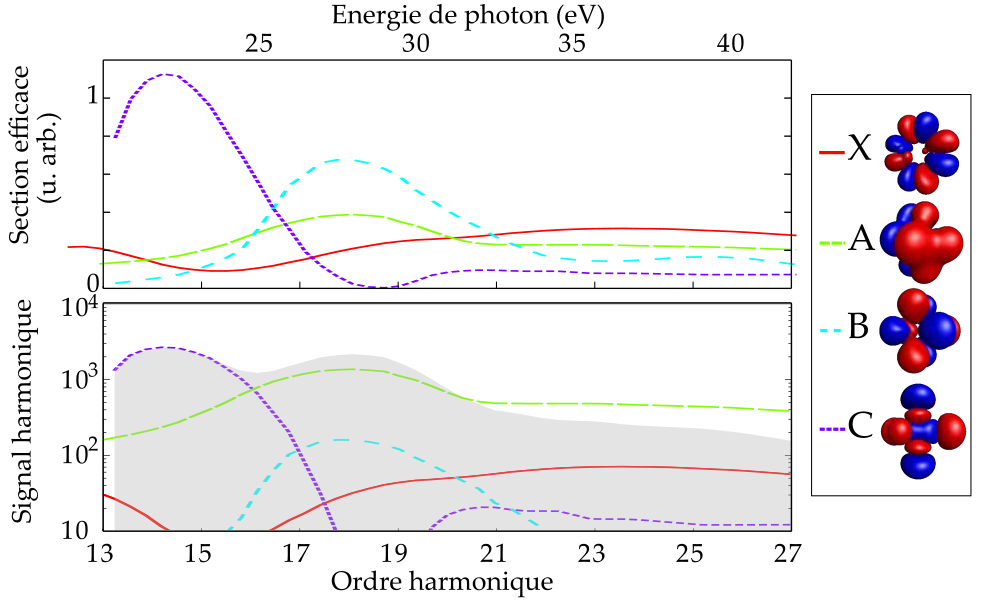
\includegraphics[width=.8\columnwidth]{Figures/SF6/sf6_cross_section.png}%
\caption{(Haut) Section efficace de photoionisation XUV de différents canaux d'ionisation. Extrait de \mycite{Yang98}. (Bas) Intensités des harmoniques générées par chaque canal, obtenues numériquement. La zone grisée est la superposition cohérente de tous les canaux d'ionisation. La longueur d'onde du champ de génération est 800 nm. (Droite) Orbitales moléculaires correspondant à chaque canal. Tiré de \mycite{FerreNC2015}.}
\label{fig:sf6_cross_section}
\end{figure}

Nous avons mesuré l'ellipticité apparente du rayonnement dans cette gamme spectrale en utilisant le polariseur décrit plus haut. Les résultats sont présentés sur la figure \ref{fig:sf6_ell}. Dans un premier temps, on utilise un champ de génération à 800 nm. On observe de très hautes valeurs d'ellipticité pour les harmoniques résonantes, atteignant presque 0.8 pour l'harmonique 15 avec seulement une ellipticité de génération de 0.2. 

\begin{figure}[!ht]
\centering
\def\svgwidth{1\columnwidth}
\import{Figures/SF6/}{sf6_ellipticite.pdf_tex}
\caption{En haut, signal harmonique produit dans \sf6 en variant l'ellipticité de génération $\epsilon_0$. En marron à jaune, impulsions de 800 nm, $\SI{1.3e14}{W/cm^2}$. En bleu foncé à clair, impulsions de 400 nm, $\SI{1.0e14}{W/cm^2}$. En bas, ellipticité apparente du rayonnement harmonique. L'erreur sur la mesure, déterminée en répétant les mesures, est de $\pm0.03$.}
\label{fig:sf6_ell}
\end{figure}

Pour les mêmes raisons qu'expliqué auparavant, il est avantageux d'utiliser un laser de génération à 400 nm. L'expérience montre que l'on garde une ellipticité très satisfaisante : les harmoniques 5 et 7 portent respectivement une ellipticité de $\simeq 0.75$ et $\simeq 0.5$ avec $\epsilon_0=0.45$. On dispose ainsi d'une source aux propriétés remarquables, le flux étant amélioré par la génération à 400 nm. Une mesure par une photodiode calibrée montre que l'harmonique 5 contient $\num{7e6}$ photons par impulsion quand $\epsilon_0=0.3$, c'est-à-dire $\num{2e9}$ photons par seconde. Cette valeur peut être encore augmentée en utilisant par exemple des impulsions plus énergétiques et une longueur focale plus élevée.

En conclusion, nous avons construit une source de rayonnement ultraviolet ultra-bref polarisé circulairement. Chaque harmonique considérée séparément a en effet une durée de l'ordre de la durée de l'impulsion de génération, c'est-à-dire $\simeq 20$ femtosecondes, ce qui en fait une alternative particulièrement intéressante aux sources synchrotrons malgré son flux moindre. Comparé aux lasers à électron libre, eux aussi capables de produire des polarisation circulaires \mycite{AllariaPRX2014}, le flux est bien sûr bien moindre, mais le taux de répétition et la résolution temporelle fournis par la GHOE sont très avantageux pour des mesures de spectroscopie moléculaire. Dans la suite nous démontrerons ce point en effectuant des expériences de photoionisation sur des molécules chirales. 
%
\chapter{Polarisation circulaire et chiralité}
\section{Définitions de la chiralité}
\subsection{Molécules chirales}
Le concept de polarisation de la lumière est historiquement lié à celui de la \textit{chiralité}. En 1808, Malus observa que la lumière réfléchie par une substance diaphane possédait une polarisation (mot qu'il introduisit en 1810). Cette polarisation était mise en évidence par une transmission à travers un cristal de calcite. Cette propriété fut observée par Arago dans des cristaux de quartz, avant d'être étudiée par Biot qui en 1812 montra que différents types de quartz tournaient la direction de polarisation soit à droite soit à gauche, propriété appelée \textit{activité optique}. Il mesura le même effet dans des substances organiques telles que des molécules de camphre. En 1848, Pasteur relia cette propriété optique à la géométrie du cristal ou de la molécule considérée. Il émit l'idée que certaines molécules existaient sous des formes géométriques dissymétriques tout en ayant les mêmes propriétés chimiques. Le mot de \textit{chiralité} fut introduit en 1893 par Lord Kelvin durant la deuxième "Robert Boyle Lecture" à l'université d'Oxford \mycite{kelvin1894} :
\begin{quotation}
I call any geometrical figure, or group of points, 'chiral', and say that it has chirality if its image in a plane mirror, ideally realized, cannot be brought to coincide with itself.
\end{quotation}
Le terme de chiralité dérive du mot grec sigifiant "main", un exemple d'objet chiral (voir figure \ref{fig:chirality}). Les deux formes possèdent un pouvoir rotatoire opposé et sont nommées \textit{énantiomères} (formes opposées en grec). On peut les nommer selon le signe de la rotation qu'ils imposent à la lumière : on parle alors de molécule dextrogyre (D ou +) ou lévogire (L ou -). Cependant, une même molécule peut imposer une rotation gauche ou droite selon la longueur d'onde de la lumière utilisée. On utilise donc également la configuration absolue de la molécule, définie à partir de sa structure tri-dimensionelle. On note alors les énantiomère R (rectus) et S (sinister). La configuration absolue d'une molécule est habituellement mesurée par diffraction X \mycite{Bijvoet1951}, par explosion coulombienne \mycite{pitzer2013} ou encore par spectroscopie micro-onde \mycite{patterson2013}.

\begin{figure}[!ht]
\centering
\includegraphics[width=.5\columnwidth]{Figures/Chirality/chirality_with_hands.pdf}%
\caption{Une molécule "chirale" n'est pas superposable à son image dans un miroir. De même que les mains gauches et droites ont un pouce et des doigts dans le même ordre, les molécules chirales ont les mêmes atomes dans le même ordre mais ne sont pas images l'une de l'autre dans un miroir.}
\label{fig:chirality}
\end{figure}

\subsection{La chiralité de la lumière}
Deux énantiomères ont les mêmes propriétés chimiques. Cependant, elles interagiront différemment avec un objet lui-même chiral. Par exemple, la plupart des récepteurs biologiques sont chiraux et réagiront très différemment à une protéine R ou S. Le contrôle et la mesure des propriétés chirales sont donc centraux dans l'industrie alimentaire, pharmaceutique et cosmétique. 

Les expériences mentionnées montrent que la lumière permet de caractériser une molécule chirale, ce qui implique que la lumière elle-même doit être un objet chiral. La définition donnée plus haut est insuffisante, car comme noté par Lord Kelvin dans ses \textit{Baltimore Lecture}, elle ne permet pas de distinguer les effets due à la chiralité de ceux dues à d'autres types de dissymétries telles que l'effet Faraday. \mycite{Barron1986} donne une définition généralisable à la chiralité de particules élémentaires telles qu'un photon :

\begin{quotation}
True chirality is exhibited by systems that exist in two distinct enantiomeric (enantiomorphic) states that are interconverted by space inversion, but not by time reversal combined with any proper spatial rotation.
\end{quotation}

Cette définition permet de distinguer la "vraie" chiralité de la fausse, c'est-à-dire une chiralité indépendante du temps. Les opérations spatiales et temporelles décrites sont représentées sur la figure \ref{fig:truefalsechir}, où elles sont notées T (inversion du temps), P (inversion de l'espace), et $\text{R}_{\pi}$ (rotation, ici d'angle $\pi$). 

\begin{figure}[!ht]
\centering
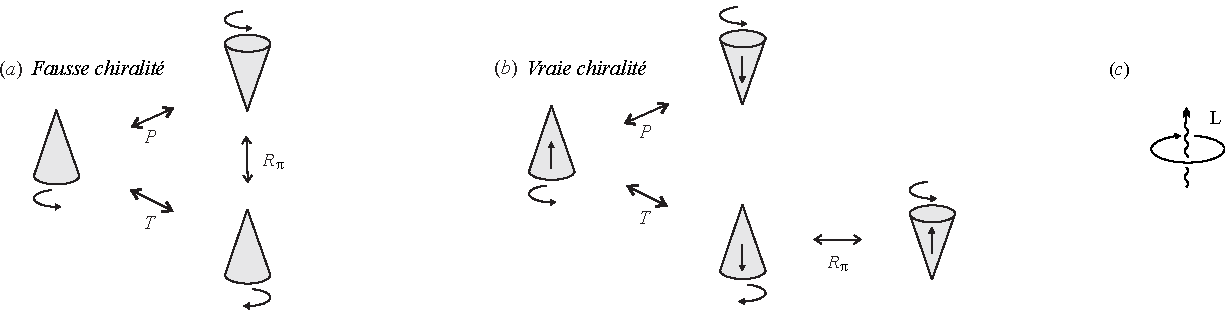
\includegraphics[width=.9\columnwidth]{Figures/Chirality/truefalsechir.pdf}%
\caption{Vraie et fausse chiralité. \textit{(a)} Cône en rotation immobile. P (inversion de l'espace) donne le même résultat que T (inversion du temps) suivi de $\text{R}_{\pi}$ (rotation d'angle $\pi$). \textit{(b)} Cône en rotation en translation. Il présente cette fois une vraie chiralité. \textit{(c)} Lumière polarisée circulairement : un photon est analogue au cône en translation. Tiré de \mycite{barron}.}
\label{fig:truefalsechir}
\end{figure}

Dans cette figure, on prend l'exemple d'un cône en rotation. Si le cône est immobile, P donne la même chose que T suivi de $\text{R}_{\pi}$, il ne présente pas de vraie chiralité. Au contraire, s'il est en translation, il a une vraie chiralité. Le cas du photon est similaire, l'hélicité du photon pouvant être vue classiquement comme une rotation. Le photon ne peut de plus pas être immobile, la lumière polarisée circulairement est donc chirale selon cette définition. Pour des molécules chirales, on appelle mélange \textit{racémique} un mélange composé d'autant de chacun des deux énantiomères. Ceci est analogue à une lumière polarisée linéairement, constituée d'autant de photons polarisés circulairement droit que gauche. 

La lumière polarisée circulairement est donc un outil de choix pour sonder et caractériser les molécules chirales. De nombreuses interactions sont possibles, nous décrirons dans la section suivante celle nommée dichroïsme circulaire, avant de présenter le dichroïsme circulaire de photoélectron, que nous mesurerons avec la source décrite dans la partie \ref{CH:Circular_HHG}.

\section{Dichroïsme circulaire d'absorption}
Fresnel expliqua le phénomène d'activité optique par une différence de vitesse de propagation de la composante circulaire droite (notée D) et gauche (G) d'une onde polarisée linéairement. Le milieu présente donc un indice de réfraction pour chaque composante. Considèrons un champ polarisé linéairement tel que les vecteurs champs électriques RCP et LCP soient parallèles à $z = 0$. Après une propagation sur une distance $L$, les champs auront tourné de $\theta^{G}=2\pi\rmc L/(\lambda v^{G})$ et $\theta^{R}=-2\pi\rmc L/(\lambda v^{RCP})$. L'angle de rotation de la direction du champ s'écrit alors :
\begin{align*}
\chi = \frac{1}{2}(\theta^{G}+\theta^{D}) &= \frac{\pi\rmc L}{\lambda}\left(\frac{1}{v^{G}}-\frac{1}{v^{D}}\right)\\
&= \frac{\pi}{\lambda}\left(n^{G}-n^{D}\right).
\end{align*}

Mais si $n^{G}$ et $n^{D}$ sont différents, le milieu doit également absorber différemment chaque composante du champ. Cet effet a été mesuré pour la première fois par \mycite{Haidinger1847} puis étudié par \mycite{Cotton1895}, qui le nomma \textit{dichroïsme circulaire}. Cet effet est toujours couramment utilisé avec des longueurs d'ondes visibles ou infrarouges. Il est généralement préféré à la mesure de l'activité optique car il évolue plus rapidement avec la longueur d'onde, et permet donc de distinguer plus facilement différentes bandes spectrales. Le dichroïsme circulaire est ainsi utilisé pour la détermination de structures de protéines, de changements de structures induits par par exemple le pH ou le solvant, de repliements/dépliements de protéines, ou encore de liaison de ligands.

L'absorption correspond à une transition d'un état initial vers un état excité. Lorsque la lumière traverse un ensemble de molécule, son intensité est gouvernée par la loi de Beer-Lambert, c'est-à-dire une décroissance exponentielle en fonction de la longueur parcourue. On note $\alpha^{D}$ et $\alpha^{G}$ les coefficients d'absorption de chacune des composantes du champ. Le dichroïsme circulaire vaut :
\[\Delta \alpha = \alpha^{G}-\alpha^{D}.\]
En pratique, on préfère utiliser le ratio entre le dichroïsme circulaire et l'absorption habituelle, appelé facteur de dissymétrie \mycite{Kuhn1930} : 
\begin{equation}
g = \frac{\alpha^{G}-\alpha^{D}}{\frac{1}{2}(\alpha^{G}+\alpha^{D})}.
\label{eq:kuhn}
\end{equation}

Relions $\alpha$ aux propriétés de la molécule. Pour une longueur de propagation $\delta z$ dans le milieu infinitésimale, l'intensité absorbée par unité de surface $\delta I$ s'écrit :
\begin{align*}
\frac{\delta I}{I} = \alpha c \delta z,
\end{align*}
où $c$ est le nombre de molécule par mètre cube. On note $w$ l'énergie moyenne absorbée par molécule, on a donc $\delta I = c \delta z w$. On obtient alors :
\begin{align}
\alpha = \frac{\delta I}{Ic \delta z} = \frac{c \delta z w}{Ic \delta z} = \frac{w}{I}.
\label{eq:cd1}
\end{align}
Notons qu'un facteur de proportionnalité s'ajoute à cette expression si on choisit d'utiliser un coefficient d'absorption molaire.

Considérons maintenant la transition électronique $i\rightarrow f$. \`A cette transition est associé un élément de matrice de transition qu'on note $V_{if}$. La bande d'absorption a un profil spectral qui donne la probabilité de transition en fonction de la fréquence, qu'on note $\rho(\omega)$. \mycite{schellman1975} montre que ces quantités sont reliés à $w$ par la relation :
\begin{equation}
w(\omega) = \frac{\pi \omega |V_{if}|^2 \rho(\omega)}{2\hbar}.
\label{eq:cd2}
\end{equation}

Il faut donc déterminer $V_{if}$ pour obtenir $\alpha$. Commençons dans l'approximation dipolaire électrique. Dans ce cas, le champ électrique se couple avec le moment dipolaire de la molécule : $V_{if} = -\bm{\mu}_{if}\cdot \bm{E}$, où $\mu_{if}$ est le moment dipolaire (voir partie \ref{sec:multipolar}). \mycite{schellman1975} montre que si le champ est polarisé circulairement droite ou gauche, on a $(V_{if}^{D/G})^2 = (\bm{\mu}_{if})^2E^2_0/3$, où la division par 3 provient d'une moyenne sur les orientation possibles des moments dipolaires.
On utilise alors les équations \ref{eq:cd1} et \ref{eq:cd2} :
\begin{align*}
\alpha^{D/G}(\omega) &= \frac{w^{D/G}(\omega)}{I} = \frac{\pi \omega |V_{if}^{D/G}|^2 \rho(\omega)}{2\hbar I} 
= \frac{\pi \omega |\mu_{if}E_0|^2 \rho(\omega)}{6\hbar I} 
= \frac{\pi \omega |\mu_{if}|^2 \rho(\omega)E^2_0}{6\hbar I} \\
&= \frac{4\pi^2 \omega |\mu_{if}|^2 \rho(\omega)}{3\hbar n \rmc} 
\end{align*}
On obtient donc directement le dichroïsme circulaire : $\Delta\alpha = \alpha^G-\alpha^D = 0$. Dans l'approximation dipolaire, le dichroïsme circulaire est donc nul. \par Il faut considérer le terme suivant du développement multipolaire : 
\[V_{if} = -\bm{\mu}_{if}\cdot \bm{E} - \bm{m}_{if}\cdot \bm{B}.\] 
\mycite{schellman1975} réalise le calcul de $V_{if}$ pour une polarisation circulaire :
\begin{align*}
(V_{if}^{D/G})^2 &= \frac{(\bm{\mu}_{if})^2E^2_0}{3}+\frac{(\bm{m}_{if})^2B^2_0}{3} \mp \frac{2}{3}\text{Im}(\bm{\mu}_{if}\cdot\bm{m}_{if})E_0B_0 \\
&= \frac{8\pi I}{3 \rmc}\left[\frac{(\bm{\mu}_{if})^2}{n} +  n(\bm{m}_{if})^2 \mp 2 \text{Im}(\bm{\mu}_{if}\cdot\bm{m}_{if})\right]. 
\end{align*}
Chacun des trois terme a sa propre probabilité de transition, qu'on note $\rho(\omega)$, $\tau(\omega)$ et $\sigma(\omega)$. On obtient donc pour le coefficient d'atténuation :
\begin{equation*}
\alpha^{D/G}(\omega) = \frac{4\pi^2 \omega}{3\hbar \rmc}\left[\frac{\rho(\omega)(\bm{\mu}_{if})^2}{n} +  n\tau(\omega)(\bm{m}_{if})^2 \mp 2 \sigma(\omega)\text{Im}(\bm{\mu}_{if}\cdot\bm{m}_{if})\right] 
\end{equation*}

Les trois termes obtenus correspondent à l'absorption dipolaire électrique, l'absorption dipolaire magnétique, et le dichroïsme circulaire. En effet, on obtient :
\[ \Delta \alpha = \alpha^G-\alpha^D = \frac{16\pi^2 \omega\sigma(\omega)\text{Im}(\bm{\mu}_{if}\cdot\bm{m}_{if})}{3\hbar \rmc}. \]
Le fait que l'on ait besoin d'utiliser l'approximation dipolaire magnétique pour observer du dichroïsme circulaire signifie que cet effet sera faible en général. Ainsi, le facteur d'asymétrie $g$ (équation \ref{eq:kuhn}) a des valeurs typiques de $10^{-5}\text{-}10^{-3}$ \mycite{Levi1980}. Ceci impose de réaliser des mesures à densité élevée, c'est-à-dire en phase liquide ou sur des films minces. La mesure est alors parasitée par la contribution du solvant ou du substrat, empêchant la mesure du dichroïsme de la molécule libre.
\clearpage
\section{Dichroïsme circulaire de photoélectron (PECD)}
\label{sec:PECD}
On s'intéresse désormais à un autre type de dichroïsme, qui comme nous allons voir a des propriétés très différentes. Jusque ici, nous avons présenté des techniques chiroptiques (terme désignant l'étude de molécule chirales par la lumière) dans le domaine visible ou proche infrarouge. Le passage à des énergies de photon plus élevées donne accès à un phénomène supplémentaire : la photoionisation. Nous allons donc décrire l'émission d'un électron par une molécule chirale suite à l'absorption de lumière polarisée circulairement. 

On considère une impulsion lumineuse se propageant selon la direction $e_z$. On place une molécule chirale au centre d'un repère sphérique $(r,\theta,\phi)$, où $r$ est la position du photoélectron, $\theta$ est l'angle par rapport à l'axe $e_z$, comme représenté sur la figure \ref{fig:geomPECD}.

\begin{figure}[!ht]
\centering
\def\svgwidth{0.5\columnwidth}
\import{Figures/PECD/}{geomPECD.pdf_tex}
\caption{Géométrie de photoionisation.}
\label{fig:geomPECD}
\end{figure}

Dans le cas de molécules chirales d'orientation aléatoire et d'un champ parfaitement polarisé, le phénomène ne dépend pas de $\phi$. En 1976, \mycite{RitchiePRA1976} obtint l'expression de la distribution angulaire des photoélectrons éjectés et montra qu'elle prend la forme suivante :
\begin{equation}
I^p(r,\theta) = b_0^p(r) + b_1^p(r) P_1(\cos\theta) + b_2^p(r) P_2(\cos\theta)
\label{eq:angulardistrib}
\end{equation}
où les $b_i$ sont des fonctions du potentiel moléculaire, de l'énergie $h\nu$ et de la polarisation $p$ du photon incident ($p = 0$, polarisation linéaire, $p =\pm1$ polarisation circulaire gauche/droite). Les $P_i$ sont les polynômes de Legendre, qui valent $P_1(x) = x$ et $P_2(x) = (3x^2-1)/2$. Il est important de noter que contrairement à celui du dichroïsme circulaire, ce calcul a été réalisé dans l'approximation dipolaire électrique. Le calcul complet des $b_i$ permet d'obtenir les propriétés suivantes :
\begin{align}
b_0^1 &= b_0^{-1} \nonumber\\
b_1^0 &= 0\nonumber\\
b_1^1 &= -b_1^{-1}\nonumber\\
b_2^1 &= b_2^{-1}.
\label{eq:bi}
\end{align}
$b_0$ est couramment appelé PES (Photo Emission Spectrum), et correspond simplement à la section efficace de photoionisation de la molécule. $b_2$ est souvent noté $\beta$ et appelé paramètre d'anisotropie. Quant à $b_1$, on remarque qu'il fait apparaître un dichroïsme :
\begin{equation}
I^{1}(r,\theta)-I^{-1}(r,\theta) = (b_1^1(r)-b_1^{-1}(r))P_1(\cos\theta) = 2b_1^1(r)\cos\theta
\label{eq:pecddef}
\end{equation}
On obtient donc une asymétrie autour de $\theta = 90\degres$, c'est-à-dire avant-arrière par rapport à la direction de propagation de la lumière. Cet effet est appelé dichroïsme circulaire de photoélectron (PECD, \textit{PhotoElectron Circular Dichroism}), et $b_1$ est le \textit{paramètre dichroïque}. On note souvent $PECD = 2b_1$. L'équation \ref{eq:bi} montre directement que le PECD change de signe si on change l'hélicité de la lumière. De même, le signe change si on change d'énantiomère.

\mycite{PowisJPCA2000} obtint théoriquement des asymétries allant jusqu'à 40\% de la section efficace totale. Des démonstrations expérimentales n'ont pas tardé à arriver, profitant du développement de sources synchrotrons fournissant de la lumière XUV polarisée circulairement. \mycite{BoweringPRL2001} ont mesuré le PECD du bromocamphre en 2001, avant que \mycite{GarciaJCP2003} étudient le camphre et \mycite{TurchiniJACS2004} le methyloxirane. L'asymétrie la plus haute aujourd'hui mesurée est de 32\% \mycite{DalyJCP2011}. Ces valeurs élevées s'expliquent par le caractère purement dipolaire électrique du PECD et permettent de réaliser des études chiroptiques en phase gazeuse.
Par la suite, l'étude du PECD a montré son impressionnante sensibilité aux finesses du potentiel moléculaire. Tout d'abord, $b_1$ est différent selon l'orbitale ionisée, comme démontré dans le camphre par \mycite{NahonJCP2006}. Ensuite, le PECD peut varier drastiquement avec des substitutions chimiques, comme illustré sur la figure \ref{fig:substitution}, tirée de \mycite{Tia2014}. On y voit qu'en changeant un élément de la molécule, la section efficace et le paramètre $\beta$ ne changent presque pas, car l'orbitale ionisée est localisé sur l'atome d'oxygène. Cependant, le paramètre $b_1$ évolue drastiquement, permettant de différencier les quatres molécules. Un autre exemple est celui des conformères, qui sont des molécules de même formule mais dont les atomes ont tourné autour d'une liaison chimique. Le PECD est également capable de distinguer ces deux molécules \mycite{GarciaPCCP2008}. Pour finir, il a récemment été observé que le PECD était sensible aux modes de vibration, c'est-à-dire aux mouvements des noyaux \mycite{GarciaNC2013}.

\begin{figure}[!ht]
\centering
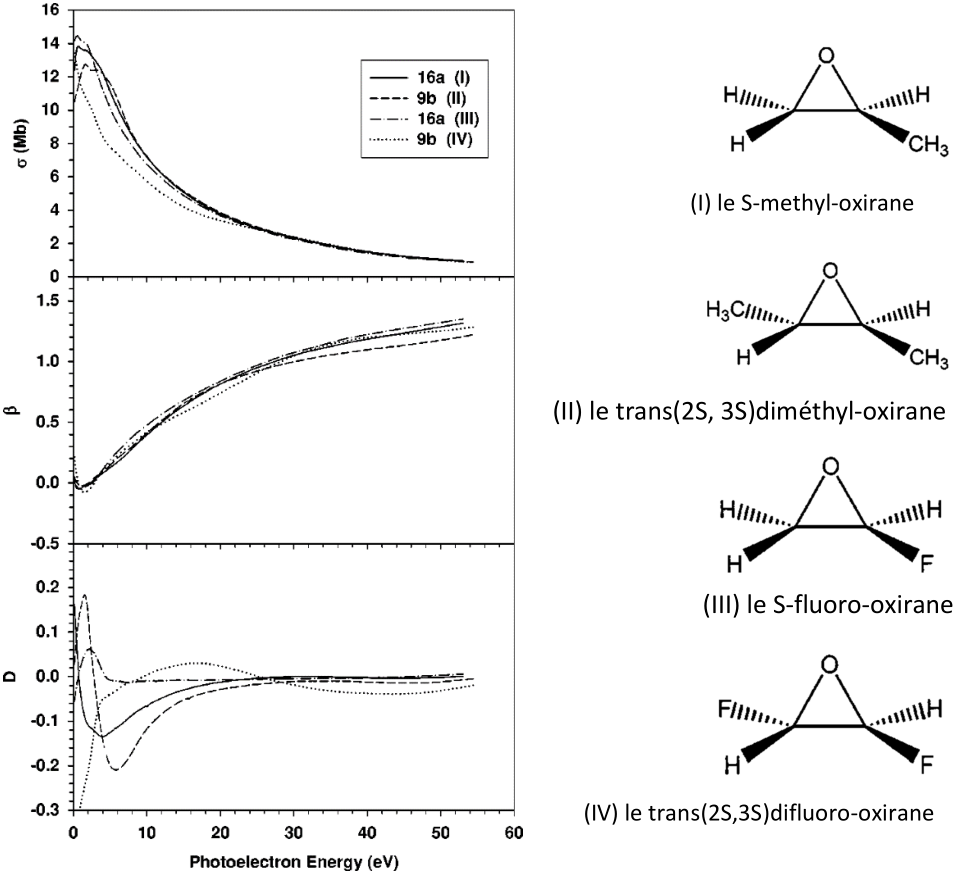
\includegraphics[width=.7\columnwidth]{Figures/PECD/substitution.png}%
\caption{Effet d'une substitution sur le PECD. Quatres molécules sont représentées à droite. \`A gauche, on voit leur section efficace de photoionisation $\sigma$, leur paramètre d'anisotropie $\beta$ et le paramètre dichroïque $b_1$, ici noté D. Tiré de \mycite{Tia2014}.}
\label{fig:substitution}
\end{figure}

Cette haute sensibilité au détails fins du potentiel moléculaire peut être expliquée dans un modèle où un électron diffuse sur la molécule après avoir été ionisé. On part d'un état initial où l'électron est lié, et on observe l'électron dans le continuum après qu'il ait diffusé sur le potentiel moléculaire. \mycite{DillDehmer1974} montrent que la fonction d'onde du photoélectron dans le continuum se décompose en différentes composantes de moment angulaire défini. Chacune de ces composante est déphasée différemment par le potentiel moléculaire. La phase de chaque composante $\ell$, que l'on note $\sigma_\ell$, est responsable d'interférences dans le continuum entre ondes partielles. Ainsi, une observable sera d'autant plus sensible au potentiel moléculaire qu'elle est sensible à des petites variations de $\sigma_\ell$. Le calcul de \mycite{RitchiePRA1976} donne les dépendances en $\sigma_\ell$ des $b_i$ :

\begin{itemize}
\renewcommand{\labelitemi}{$\bullet$}
\setlength\itemsep{1em}
\item $b_0$ ne dépend pas du tout de $\sigma_\ell$. La section efficace intégrée sur tout l'espace ne présente donc que peu d'information.
\item $b_2$ dépend de $\sigma_\ell$ pour une valeur de $\ell$ sur deux. Plus précisément, $b_2$ présente un terme $\cos(\sigma_\ell-\sigma_{\ell+2})$. $b_2$ fournit donc davantage d'information que la section efficace totale.
\item Le cas qui nous intéresse est celui de $b_1$, qui lui présente un terme $\sin(\sigma_\ell-\sigma_{\ell+1})$. Toutes les composantes $\ell$ influent donc sur sa valeur. De plus, on a une dépendance en sinus, qui varie significativement pour des petites valeurs de déphasage entre composantes $\ell$. Au contraire, le cosinus dans l'expression de $b_2$ est relativement plat au voisinnage de $\sigma_\ell-\sigma_{\ell+2} = 0$.
\end{itemize}

Nous avons jusque ici mentionné des études réalisées sur synchrotron. Ces travaux présentent une très bonne résolution spectrale, mais faute de source adaptée, aucune étude \textit{dynamique} du PECD n'a été réalisée. Nous allons utiliser la source présentée en partie \ref{CH:Circular_HHG} à cet effet.
%
\chapter{Mesures de PECD avec une source d'harmoniques d'ordre élevé}
\section{Dispositif expérimental}
\subsubsection{Source de lumière}
Nous utilisons la source décrite en partie \ref{CH:Circular_HHG}, dont nous rappelons brièvement les propriétés : le système laser Aurore délivre des impulsions à $\simeq$800 nm, qui sont doublées dans un cristal de BBO de type 1 de 200 $\si{\micro\metre}$. On dispose alors d'impulsions de 1 mJ à 404 nm à une fréquence de 1 kHz. Pour mesurer un PECD, il est pratique d'alterner successivement polarisations circulaires droite et gauche et de faire la différence entre elles, de sorte à éviter des effets de dérive lente. Pour ce faire, il faut alterner la polarisation du champ de génération à 404 nm. On utilise une lame demi-onde d'ordre 0 large bande placée avant une lame quart d'onde. L'orientation de la lame quart d'onde est fixe selon l'axe vertical. On peut ainsi tourner la lame demi-onde d'un angle $\pm\beta/2$ pour obtenir une ellipticité $\epsilon_0 = \pm \tan\beta$, tout en gardant l'axe de l'ellipse vertical après les lames d'onde. On choisit ici $\epsilon_0 = \pm 0.3$. La figure \ref{fig:waveplates} illustre le fonctionnement du dispositif. Le rayonnement est ensuite focalisé dans un jet de \sf6 par lentille de $\text{SiO}_2$ de 50 cm de focale. Les harmoniques générées sont alors polarisées elliptiquement et d'ellipticité de même signe que celui du fondamental. Les valeurs d'ellipticité apparentes ont été présentées plus haut (voir figure \ref{fig:sf6_ell}).

\begin{figure}[!ht]
\centering
\def\svgwidth{0.7\columnwidth}
\import{Figures/PECD/}{waveplates.pdf_tex}
\caption{Contrôle de l'état de polarisation du fondamental. De gauche à droite : état de polarisation avant les lames d'onde, état après une lame demi-onde d'angle $\pm\beta/2$, état après une lame quart d'onde orientée verticalement.}
\label{fig:waveplates}
\end{figure}

\subsubsection{Détection : spectromètre imageur de vecteur vitesse}
Le champ harmonique produit par les molécules de \sf6 est alors utilisé pour photoioniser un gaz de molécules chirales. Pour ne pas modifier l'état de polarisation du champ, on n'introduit aucune optique entre la source et la zone de détection. Seul un iris permet d'ajuster l'intensité envoyée dans le gaz de molécule. La mesure du PECD de ces molécules nécessite de connaître l'énergie et la direction d'émission des photoélectron créés lors de la photoionisation. Expérimentalement, ceci est réalisé à l'aide d'un spectromètre imageur de vecteur vitesse (VMI pour \textit{Velocity Map Imager}). 

Le fonctionnement de cet appareil est représenté sur la figure \ref{fig:vmi}. Le faisceau harmonique croise un jet moléculaire, dont le recouvrement définit la zone d'interaction. La photoionisation a lieu dans cette zone, et crée un nuage d'espèces chargées (ions et électrons). Autour de cette zone sont positionnées trois électrodes servant à collecter ces espèces chargées. Ces électrodes forment une \textit{lentille électrostatique} qui vient focaliser les espèces chargées sur un détecteur placé perpendiculairement à l'axe de propagation de la lumière, constitué de galettes de micro-canaux (MCP) et d'un écran de phosphore. L'électrode la plus éloignée du détecteur repousse les espèces et est donc appelée répulseur. L'électrode intermédiaire est appelée extracteur, tandis que la troisième est l'électrode de masse car son potentiel est nul. Le signe des potentiels permet de collecter les ions ou bien les électrons émis lors de l'interaction. 

\begin{figure}[!ht]
\centering
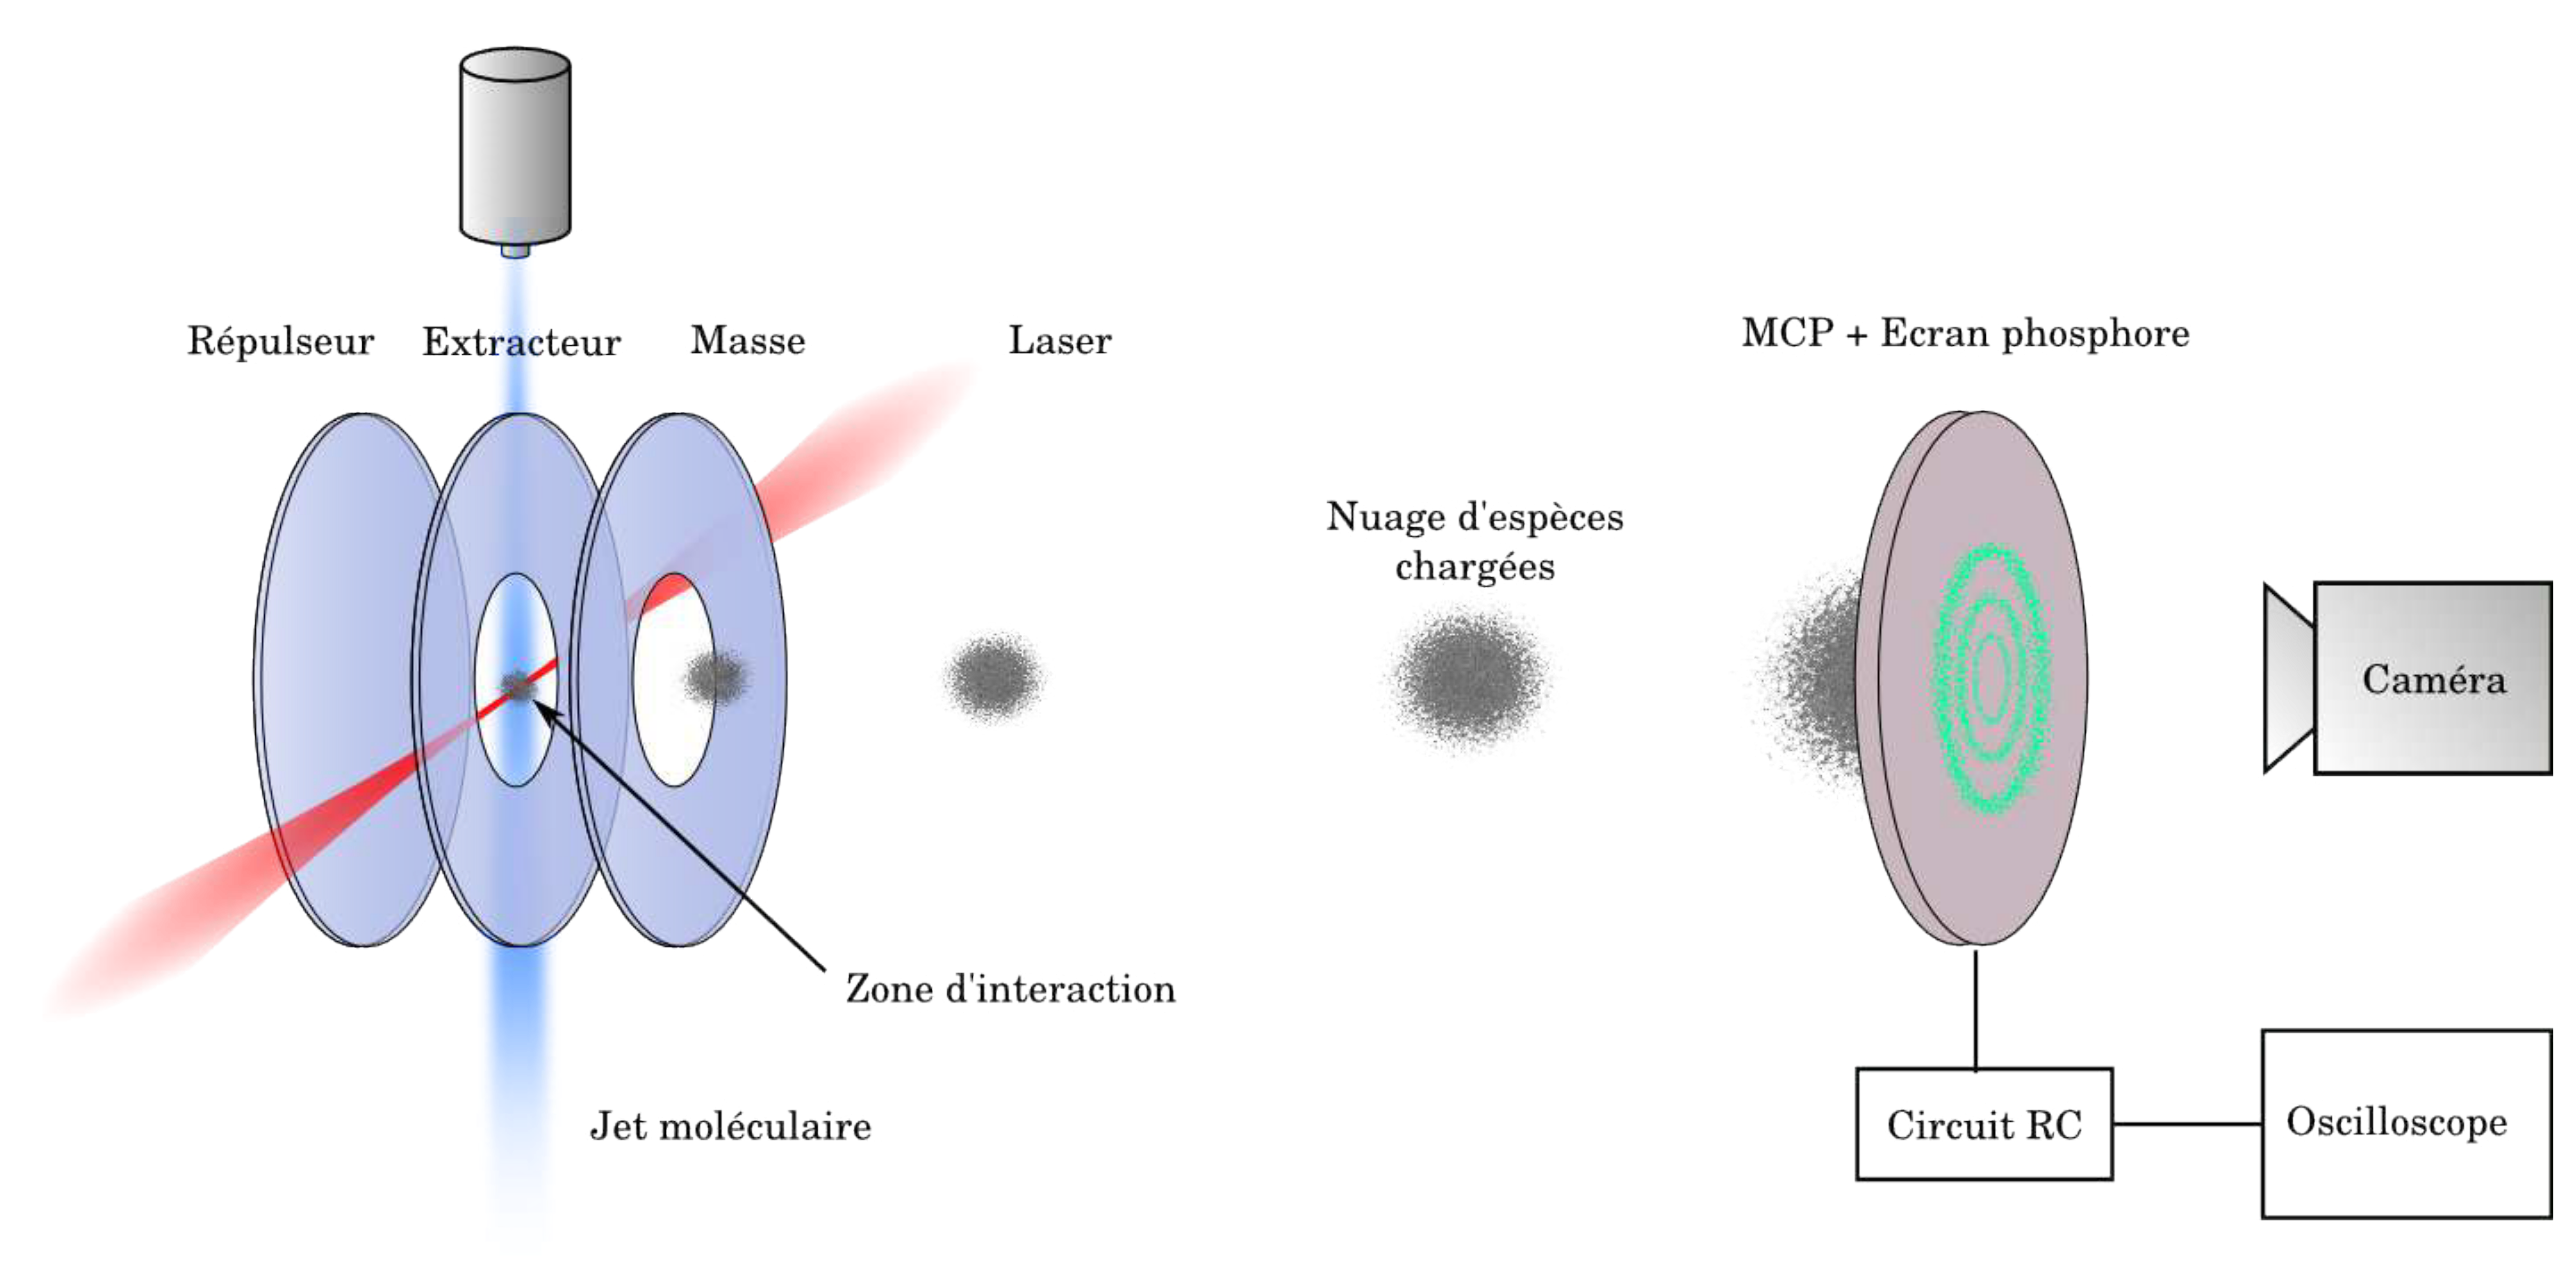
\includegraphics[width=1\columnwidth]{Figures/PECD/vmi.png}%
\caption{Schéma représentatif du fonctionnement d'un VMI (Spectromètre imageur de vecteur vitesse). Tiré de \mycite{handschin}.}
\label{fig:vmi}
\end{figure}

Les deux dernières électrodes de l'appareil sont percées en leur centre, amélioration majeure proposée par \mycite{EppinkParker1997}. L'instrument ainsi réalisé possède des propriétés remarquables. D'abord, les particules sont collectées dans un angle solide avoisinant les $4\pi$ stéradians. De plus, quand la lentille électrostatique est optimisée, toutes les particules de même vecteur vitesse sont focalisées en un unique point du détecteur, quelque soit le lieu où elles ont été émises. C'est cette propriété qui donne son nom à ce spectromètre de vecteur vitesse. On trouvera une discussion très détaillée sur la conception de cet appareil dans la thèse de C. Handschin \mycite{handschin}.

\section{Résultats dans la fenchone}
\label{sec:results_fenchone}
Nous choisissons un système déjà étudié sur synchrotron : la molécule de fenchone ($\text{C}_{10}\text{H}_{16}\text{O}$). Elle possède deux énantiomères, représentés sur la figure \ref{fig:fenchone}. On notera Fenchone (+) l'énantiomère de nom systématique  (1S,4R)-1,3,3-triméthylbicyclo[2.2.1]heptan-2-one et Fenchone (-) l'énantiomère (1R,4S)-1,3,3-triméthylbicyclo[2.2.1]heptan-2-one. L'orbitale moléculaire la plus haute occupée (HOMO) est d'énergie $\simeq$8.6 eV. Les suivantes sont HOMO-1 (10.4 eV), HOMO-2 (10.7 eV), HOMO-3 (11.2 eV), etc. Les valeurs de potentiel d'ionisation ont été obtenus expérimentalement sur synchrotron \mycite{PowisCPC2008}. On voit donc que la troisième harmonique, d'énergie 9 eV, est suffisante pour ioniser la HOMO.

\begin{figure}[!ht]
\centering
\def\svgwidth{0.7\columnwidth}
\import{Figures/PECD/}{fenchone.pdf_tex}
\caption{\'{E}nantiomères de la molécule de fenchone.}
\label{fig:fenchone}
\end{figure}

Pour la mesure de PECD, nous avons utilisé un VMI initialement développé par Valérie Blanchet et Charles Handschin. Un réservoir rempli d'un des deux énantiomères (fourni par Sigma-Aldrich, pureté énantiomérique $\simeq$99\%) est connecté à une buse métallique chauffée à 120\degres C de 300 $\si{\micro\metre}$ de diamètre, placée à 7 cm de la zone d'interaction. 

\begin{figure}[!ht]
\centering
\def\svgwidth{0.8\columnwidth}
\import{Figures/PECD/}{Setup_pecd.pdf_tex}
\caption{Principe de mesure de PECD avec une source d'harmoniques elliptiques.}
\label{fig:pecdsetup}
\end{figure}

La figure \ref{fig:pecdsetup} illustre le principe de l'intégralité du dispositif de mesure de PECD. On alterne successivement polarisation elliptique droite et gauche, en accumulant à chaque fois le signal pendant une dizaine de minutes. On fait ensuite la moyenne de toutes les images obtenues pour chaque polarisation, pour obtenir les grandeurs $I^{1}(r,\theta)$ et $I^{-1}(r,\theta)$, en reprenant les notations de la partie \ref{sec:PECD}. L'approche la plus directe consiste à calculer un paramètre d'asymétrie de Kuhn (voir équation \ref{eq:kuhn}) :
\[g(r,\theta) = 2\frac{I^{1}(r,\theta)-I^{-1}(r,\theta)}{I^{1}(r,\theta)+I^{-1}(r,\theta)}\]

On obtient alors l'image présentée en figure \ref{fig:asym_diff}. Les images des deux énantiomères sont presque parfaitement miroirs l'une de l'autre, ce qui valide la technique de mesure et démontre la qualité de notre source harmonique. Sur une image VMI, la coordonnée radiale $r$ est relié à l'énergie des photoélectrons détectés par une loi de la forme $E = a_0 r^2$. La constante $a_0$ est déterminée en mesurant la section efficace d'une espèce connue, dans notre cas l'argon. Cette constante dépend des tensions appliquées aux électrodes, c'est-à-dire de la focale de la lentille électrostatique du VMI. L'énergie maximale mesurable est donc déterminée par cette focale ainsi que par la taille du détecteur. 

\begin{figure}[!ht]
\centering
\def\svgwidth{0.8\columnwidth}
\import{Figures/PECD/}{asym_diff.pdf_tex}
\caption{Mesure de l'asymétrie avant-arrière pour les deux énantiomères de la fenchone étudiés. Extrait de \mycite{ferre}.}
\label{fig:asym_diff}
\end{figure}

Sur la figure \ref{fig:asym_diff}, on observe un pic d'asymétrie très fort ($\simeq$5\%) proche du centre, c'est-à-dire correspondant à des photoélectrons d'énergie faible. On distingue ensuite trois anneaux concentriques supplémentaires d'énergie plus élevée. Ces différents anneaux correspondent à des photoélectrons provenant de différentes orbitales moléculaires et/ou ionisés par des harmoniques différentes. On observe des inversions de signe entre les anneaux, résultat de la sensitivité du PECD aux états liés (i.e. orbitale ionisé) et aux états du continuum (i.e. à l'énergie de photon utilisée). 

On désire désormais extraire le paramètre $b_1(r)$ (équivalent à $b_1(E)$), ayant montré qu'il portait de nombreuses informations sur le potentiel moléculaire (voir partie \ref{sec:PECD}). Remarquons pour commencer qu'on utilise une galette de micro-canaux, détecteur à deux dimensions, pour mesurer une distribution de vecteur vitesse tridimensionnelle. Par exemple, si on suppose que les photoélectrons de même énergie sont émis de façon isotrope, on a une sphère 3D autour de la molécule ionisée, appelée sphère de Newton. Les différentes contributions donneront différentes sphères concentriques. La figure \ref{fig:sphere_projection} illustre la projection de ces sphères selon la dimension verticale $y$ ($z$ est l'axe optique et $x$ est l'axe du VMI). On voit que la projection est bien plus importante aux pôles qu'à l'équateur de la sphère. 

\begin{figure}[!ht]
\centering
\def\svgwidth{0.6\columnwidth}
\import{Figures/PECD/}{sphere_projection.pdf_tex}
\caption{Projection d'une sphère 3D sur un détecteur 2D. Une coupe selon l'axe $y$ de l'image 2D est tracée.}
\label{fig:sphere_projection}
\end{figure}

Pour passer de la figure 2D à la distribution 3D, on peut appliquer une transformée d'Abel inverse \mycite{heck1995}. Cette transformée requiert d'avoir une symétrie de révolution autour d'un axe contenu dans le plan du détecteur, ce qui est le cas de l'axe optique si on a une polarisation purement circulaire. Nous supposons donc que la polarisation du rayonnement est quasi-circulaire et utilisons un algorithme permettant de réaliser ce traitement de manière efficace, appelé pBasex \mycite{GarciaNahonPowis2004}. L'image \ref{fig:asym_diff} a été analysée en utilisant cette méthode par Gustavo A. Garcia et Laurent Nahon, ce qui dans l'approximation d'un rayonnement quasi-circulaire permet d'extraire $b_1(E)$. Le résultat est présenté sur la figure \ref{fig:pecdfenchone}, où on a noté $\text{PECD}(E) = 2b_1(E)$.

\begin{figure}[!ht]
\centering
\def\svgwidth{1\columnwidth}
\import{Figures/PECD/}{pecdfenchone.pdf_tex}
\caption{PECD mesuré dans la fenchone (+) (pointillés rouges) et (-) (traits bleus) par une source d'harmoniques produites dans \sf6par un champ à 400 nm avec $\epsilon_0=0.3$. Les lignes verticales montrent les différentes orbitales ionisés par les trois harmoniques utilisées.}
\label{fig:pecdfenchone}
\end{figure}

Dans cette figure, on observe différents maxima d'asymétrie, le premier à une énergie d'environ $3\hbar\omega - E_{HOMO}= 0.7$ eV. Les suivants sont environ à $5\hbar\omega - E_{HOMO-1}= 5.1$ eV, $5\hbar\omega - E_{HOMO}= 6.9$ eV, $7\hbar\omega - E_{HOMO-1}= 11.3$eV et $7\hbar\omega - E_{HOMO}= 13.1$ eV. Ces positions sont repérées par les pointillés verticaux. De manière intéressante, le PECD a un signe différent selon l'orbitale ionisée, ce qui est en accord avec des mesures synchrotron \mycite{PowisCPC2008} et met en avant la sensibilité du PECD. Le PECD prend des valeurs très importantes pour l'harmonique 3, ce qui peut être signe d'une très forte ellipticité. Malheureusement aucune mesure de polarimétrie optique n'a été réalisée sur cette harmonique faute de bande passante suffisante du détecteur. La question de l'état de polarisation du rayonnement sera abordée dans la partie suivante.

En conclusion, ces mesures démontrent la possibilité de mesurer un PECD à partir d'une source harmonique. Nous avons récemment étudié le phénomène de PECD dans d'autres régimes d'ionisation. En plus du régime d'ionisation à un photon présenté ici, nous avons mesuré le PECD de la fenchone en ionisation multi-photonique, en ionisation au-dessus du seuil et en ionisation tunnel. Le but est ici de démontrer l'universalité du phénomène de PECD et de montrer la complémentarité des informations obtenues dans les différents régimes d'ionisation. Nous avons de plus cherché à fournir un modèle physique commun à tous les régimes. Ces travaux font l'objet de l'article \ref{pap:BeaulieuNJP2016}, disponible à la fin du manuscrit.

Nous terminerons cette partie par une autre vision du PECD : à la place d'effectuer la spectroscopie d'une molécule grâce à la lumière, nous allons chercher à caractériser l'état de polarisation du rayonnement harmonique grâce à une molécule chirale.

\chapter{Le PECD comme outil de caractérisation du rayonnement}
\section{Le PECD en polarisation elliptique}
Jusqu'à présent, nous avons décrit le PECD en supposant que le rayonnement harmonique était quasi-circulaire. Ce n'est pas exact pour trois raisons :

\begin{itemize}
\renewcommand{\labelitemi}{$\bullet$}
\setlength\itemsep{1em}
\item L'ellipticité de chaque harmonique $\epsilon_q$ n'est pas égale à 1, comme le montrent les mesures optique de la figure \ref{fig:sf6_ell}, qui donnent une borne supérieure $\epsilon_q^{max}<1$. En terme de paramètres de Stokes, cela signifie $s_3<1$.
\item L'ellipse de polarisation du rayonnement produit par la GHOE résonante n'est pas verticale : comme le montre la figure \ref{fig:antoinepra}, l'ellipse est tournée d'un angle $\eta$ qui augmente avec l'ellipticité du fondamental $\epsilon_0$. On a donc à la fois $s_1$ et $s_2\neq 0$.
\item Le rayonnement n'est pas complètement polarisé : on a un degré de polarisation $P<1$. La valeur de $s_3$ est alors diminuée : $s_3 \rightarrow Ps_3$.
\end{itemize}


Nous devons calculer la distribution angulaire de photoélectron produite par ce rayonnement imparfait. Pour ce faire, il faut calculer la section différentielle de photoionisation dans le référentiel du laboratoire. Nous reprenons les notations de la partie \ref{sec:PECD}, où les coordonnées sphériques $(r,\theta,\phi)$ sont définies sur la figure \ref{fig:geomPECD}. Le calcul complet de la section différentielle de photoionisation dans ce cas est réalisé dans l'annexe de \mycite{ferre}. Elle est ensuite exprimée en fonction des paramètres de Stokes du rayonnement. L'expression finale est :
\begin{align}
\frac{\rmd\sigma^p}{\rmd\Omega_{\vec{k}}}(r,\theta,\phi) &\propto b_0^p(r)+s_3b_1^p(r)P_1(\cos\theta)+b_2^p(r)P_2(\cos\theta)\\
&+b_2'^p(r)\left[s_1\cos(2\phi)+s_2\sin(2\phi)\right]P_2^2(\cos\theta),
\label{eq:sigma_ell}
\end{align}

où $p=\pm1$ correspond à une polarisation elliptique gauche ou droite. On voit que $s_1$, $s_2$ et $s_3$ interviennent dans cette nouvelle expression. Dans la pratique, la mesure se fait en deux dimensions et intègre donc l'équation \ref{eq:sigma_ell} selon $\phi$. Avec notre convention d'angle, l'élément de volume infinitésimal s'écrit $\rmd V = r\rmd r \rmd \phi \sin\theta \rmd \theta$. Ainsi, l'image 2D obtenue correspond à :
\begin{equation*}
I^p(r,\theta) = \int_{\phi=0}^{2\pi}\frac{\rmd\sigma}{\rmd\Omega_{\vec{k}}}(r,\theta,\phi)\rmd\phi,
%\label{eq:sigma_ell}
\end{equation*}
On peut réécrire le terme de l'équation \ref{eq:sigma_ell} dépendant de $\phi$. On a (équation \ref{eq:stokes2}) :
\begin{align*}
s_1 &= Ps_0\cos 2\chi\cos 2\eta ,\\
s_2 &= Ps_0\cos 2\chi\sin 2\eta,
\end{align*}
où on rappelle que $\eta$ est l'angle de l'ellipse par rapport au repère cartésien, et l'ellipticité vaut $\epsilon=\tan\chi$. On réécrit donc :
\begin{align*}
\left[s_1\cos(2\phi)+s_2\sin(2\phi)\right] &= PS_0\cos 2\chi\left[\cos(2\eta)\cos(2\phi)+\sin(2\eta)\sin(2\phi)\right]\\
&= PS_0\cos 2\chi \cos(2(\phi+\eta)).
\end{align*}
Si on a une polarisation circulaire pure, $\epsilon = 1 = \tan\chi$, donc $\cos2\chi = 0$. Le terme en $b_2'$ est donc non nul seulement pour une polarisation elliptique. De plus, son intégrale selon $\phi$ s'annule. On retrouve donc l'image 2D mesurée expérimentalement :
\begin{equation*}
I^p(r,\theta) = \int_{\phi=0}^{2\pi}\frac{\rmd\sigma}{\rmd\Omega_{\vec{k}}}(r,\theta,\phi)\rmd\phi = b_0^p(r)+s_3b_1^p(r)P_1(\cos\theta)+b_2^p(r)P_2(\cos\theta),
\end{equation*}
On peut donc toujours calculer $\text{PECD} = I^1-I^{-1} = 2s_3b_1P_1(\cos\theta)$. Par contre, le terme dépendant de $\phi$ dans la section différentielle de photoionisation vient quand même briser la symétrie autour de l'axe optique. Cette brisure de symétrie est illustrée dans la figure \ref{fig:sphere_ell}. On y trace des isosurfaces de $\rmd\sigma/\rmd\Omega$, où on a choisi un profil gaussien de $b_0$, centré sur une énergie qui correspondrait à celle du photoélectron. Cette discussion ne concernant pas $b_2$, on le choisi nul, tandis que $b_1$ et $b_2'$ sont pris proportionnels à $b_0$. Leurs coefficients de proportionnalité sont choisis volontairement bien plus importants que dans un cas réel pour accentuer leurs effets. On voit que pour une polarisation linéaire, la distribution est isotrope. Pour une polarisation circulaire, elle est plus dirigée vers l'avant. Quand on considère une polarisation elliptique, on a une distribution plus complexe, non symétrique selon $\phi$ et qui dépend de $\eta$.

\begin{figure}[!ht]
\centering
\def\svgwidth{1\columnwidth}
\import{Figures/PECD/}{sphere_ellipse.pdf_tex}
\caption{Isosurfaces de la section efficace différentielle de photoionisation, pour une polarisation linéaire, circulaire et elliptique avec un angle de l'ellipse $\eta=0,\;45,\;90,\;135$\degres.}
\label{fig:sphere_ell}
\end{figure}

En conclusion, les hypothèses nécessaires à l'application des techniques usuelles d'inversion, comme pBasex, ne sont pas vérifiées. Cet algorithme ne donnera une valeur exacte que dans le cas d'une polarisation parfaitement circulaire. En particulier, il introduira un artefact sur la valeur de $b_0$, le spectre de photoémission. Par contre, $b_1$ peut toujours être retrouvé dans la différence $I^1-I^{-1}$. Pour effectuer une normalisation et exprimer $b_1$ en pourcentage, il faudrait diviser cette différence par $b_0$ mesuré en polarisation linéaire, comme suggéré dans le chapitre 5 de \mycite{ferre}.

Une fois ces précautions prises, on voit que le PECD dépend linéairement de $s_3$. En tant que phénomène chiroptique, le PECD est sensible à la \textit{vraie} ellipticité du rayonnement, contrairement aux méthodes optiques utilisées jusqu'à présent. On a donc la possibilité de caractériser complètement l'état de polarisation du rayonnement harmonique grâce au PECD. Pour ce faire, trois mesures sont nécessaires :
\begin{itemize}
\renewcommand{\labelitemi}{$\bullet$}
\setlength\itemsep{1em}
\item Une mesure de PECD de référence sur une source ayant $s_3 = 1$ et $P = 1$ à la même énergie de photon. 
\item Une mesure utilisant la source harmonique. Le rapport des PECD avec la mesure précédente donnera sa valeur de $s_3$.
\item Une mesure de loi de Malus sur la source harmonique dans les mêmes conditions, qui donnera $s_1$, $s_2$ et la borne supérieure de l'ellipticité. Le rapport entre cette borne supérieure et la véritable ellipticité donnera la valeur de $P$.
\end{itemize}
\vspace{12pt}
L'élément manquant est donc la mesure de référence sur une source complètement polarisée. Des études précédentes donnent des valeurs pour le PECD de la fenchone (\mycite{PowisCPC2008}) mais pas dans la gamme spectrale correspondant à notre spectre harmonique, en particulier aux énergies de photon faibles ($E_{H3} = 9.3$ eV). Ceci a motivé une campagne d'expériences au synchrotron SOLEIL en Février 2015, dont il est question dans la partie suivante.

\section{Mesures de référence sur synchrotron}
\subsection{La ligne DESIRS au synchrotron SOLEIL}
Sur un synchrotron, des paquets d'électrons sont d'abord accélérés dans un accélérateur linéaire avant de passer dans un onduleur, qui génère un champ magnétique perpendiculaire à la trajectoire des électrons. Le champ magnétique crée une oscillation du paquet d'électrons, qui s'accompagne d'une émission de lumière appelée rayonnement synchrotron. En jouant sur les paramètres des électrons, on peut modifier ceux de la lumière générée. Ainsi, il est possible d'obtenir un rayonnement ultra-violet intense et complètement accordable en énergie. De plus, si on applique des champs magnétiques différents selon les axes $x$ et $y$, on peut créer des oscillations selon chaque direction déphasées entre elles. On peut ainsi contrôler la polarisation de la lumière émise.

Nous avons réalisé une campagne sur la ligne DESIRS du synchrotron SOLEIL \mycite{NahonJSR2012}, ligne construite pour la spectroscopie et la mesure de dichroïsmes avec une haute résolution en énergie. Elle fournit un rayonnement d'énergie 5 à 40 eV, qui est sélectionné spectralement par une série de 4 réseaux de diffraction, permettant d'atteindre jusqu'à $\SI{54}{\micro\eV}$ de résolution à 13 eV.

Sur la ligne DESIRS, la polarisation de la lumière est contrôlée à l'aide de l'onduleur électromagnétique OPHELIE, représenté sur la figure \ref{fig:onduleur}. Les deux onduleurs croisés peuvent être translatés l'un par rapport à l'autre, de sorte à avoir un déphasage variable entre -90\degres et 90\degres. Les courants sont également ajustables pour contrôler l'amplitude des champs magnétiques appliqués. Pour la spectroscopie, il est important de caractériser l'état de polarisation de la lumière émise. Il peut varier à cause d'imperfections de l'onduleur, de la géométrie de la ligne optique, ou de dépôts sur les optiques utilisées. Pour ce faire, la ligne DESIRS est équipée d'un polarimètre VUV permettant de caractériser complètement l'état de la lumière, y compris le degré de polarisation \mycite{NahonAO2004}. Ce polarimètre est placé après un monochromateur et utilise 6 réflexions sur des prismes qui déphasent et analysent l'état du champ. Ce dispositif est unique au monde et est très efficace lorsqu'on dispose d'un flux tel que celui d'un synchrotron. Les paramètres de l'onduleur ont ainsi été optimisés jusqu'à obtenir des performances remarquables : le champ polarisé circulairement droit vérifie en moyenne $s_3/s_0=92.1\pm2.3$\% tandis que le polarisé circulairement gauche a $s_3/s_0=95.2\pm2.9$\% \mycite{NahonAO2004}.

\begin{figure}[!ht]
\centering
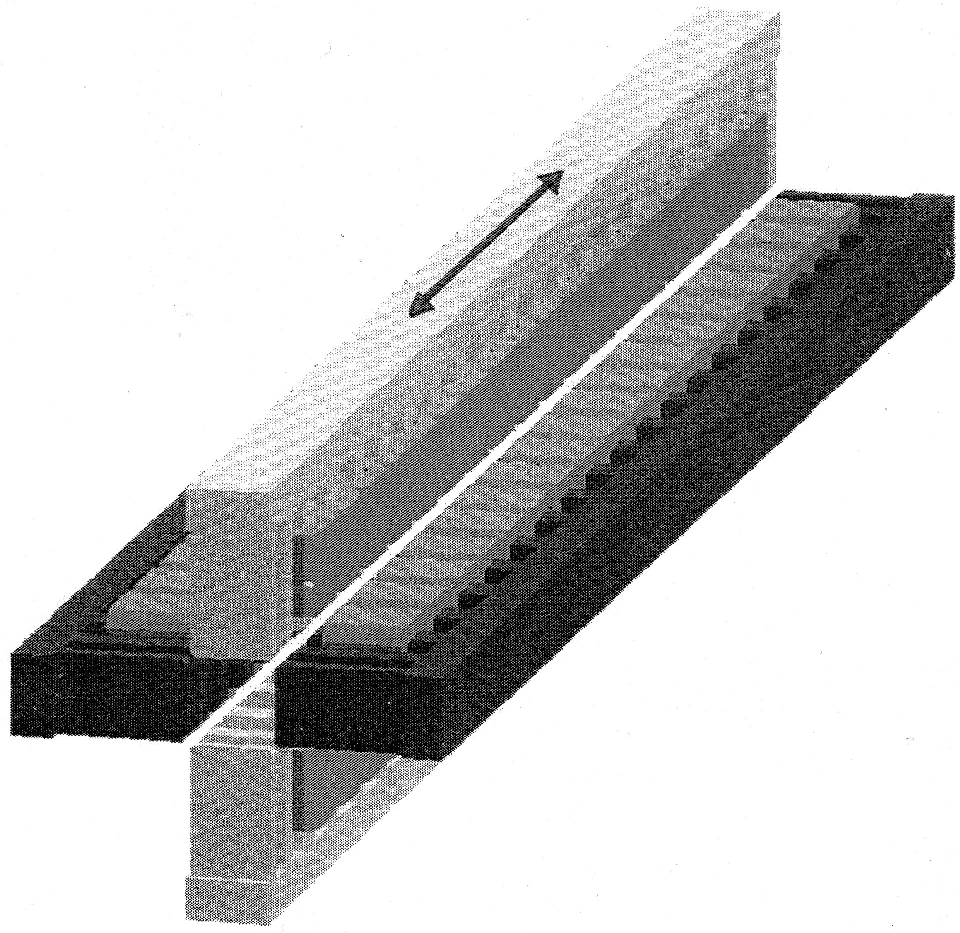
\includegraphics[width=0.4\columnwidth]{Figures/Soleil/onduleur.jpg}%
\caption{Schéma de l'onduleur croisé OPHELIE. Un onduleur peut être translaté par rapport à l'autre, permettant d'ajuster le déphasage entre les deux composantes de la lumière émise. Tiré de \mycite{NahonAO2004}.}
\label{fig:onduleur}
\end{figure}

Pour la mesure de PECD, le polarimètre est retiré et le champ est envoyé dans la zone d'interaction du spectromètre VMI Delicious. Ce spectromètre est amélioré par rapport à celui présenté plus haut car il est capable de mesurer à la fois la distribution de vecteur vitesse des électrons et le temps de vol des ions créés par le champ VUV. Le temps de vol donne la masse des ions, ce qui permet d'effectuer une analyse de corrélation et de sélectionner les électrons provenant d'une espèce donnée. On résout également les différents rapports de branchement de l'espèce chirale, même si nous ne nous sommes pas encore intéressés à cette quantité.

\subsection{Comparaison entre PECD en polarisation elliptique ou circulaire}
Commençons par étudier expérimentalement l'effet d'une polarisation elliptique sur la mesure de PECD. Comme expliqué plus haut, la polarisation du rayonnement synchrotron est modifiée en ajustant les paramètres de l'onduleur puis mesurée par le polarimètre VUV. On se place à une énergie de photon de 9.3 eV (énergie de la troisième harmonique dans la mesure réalisée au CELIA), et on choisit un rayonnement purement circulaire ou bien elliptique. Le champ elliptique a les paramètres de Stokes suivants :
\[ s_1=0.53\quad s_2=0.03\quad s_3=0.82, \]
ce qui correspond à une ellipse de polarisation tournée de $\eta=1.61$\degres~et d'ellipticité $\epsilon = 0.54$ (voir formules \ref{eq:stokes2inv}), tracée plus bas sur la figure \ref{fig:circ_ell_b0} .
 
On utilise un jet de fenchone (Sigma Aldrich). \`{A} cette énergie de photon, seule l'orbitale HOMO, d'énergie 8.6 eV, peut être ionisée. La figure \ref{fig:circ_ell_b0} présente le $b_0$ (spectre de photoémission) obtenu avec le rayonnement circulaire et elliptique. Le traitement utilise ici l'agorithme pBasex. L'échelle horizontale utilisée est l'énergie d'ionisation, définie comme $E_I = \hbar\omega - E_{\text{\'electron}}$. Les profils de $b_0$ sont remarquablement similaires. Leur amplitude est légèrement différente mais on rappelle que, pBasex ayant été utilisé, la valeur absolue de $b_0$ n'est pas correcte dans le cas elliptique.

\begin{figure}[!ht]
\centering
\def\svgwidth{0.8\columnwidth}
\import{Figures/Soleil/}{Circ_Ell_b0.pdf_tex}
\caption{Mesures de $b_0$ dans la fenchone réalisées sur la ligne DESIRS à une énergie de photon de 9.3 eV. En traits pleins, polarisation circulaire. En pointillés, polarisation elliptique. Les deux ellipses de polarisation correspondantes sont tracées à droite de la figure.}
\label{fig:circ_ell_b0}
\end{figure}

Sur la figure \ref{fig:circ_ell_b1} est représenté le paramètre dichroïque $b_1$ dans les cas circulaire et elliptique. On étudie ici la valeur de $b_1$ non normalisée par $b_0$, c'est-à-dire la simple différence $I^1-I^{-1}$. Les données pour le cas circulaire ont été prises dans la fenchone (+), tandis que celles du cas elliptique dans la fenchone (-). On a donc tracé $-b_1^{\text{circ}}$ et $b_1^{\text{ell}}$. En changeant d'énantiomère, on doit normalement mesurer une inversion parfaite de $b_1$. Au cours de cette campagne, nous avons observé une différence systématique entre les deux énantiomères. Une étude plus poussée, qui fait l'objet de l'article \ref{pap:NahonPCCP2016} \mycite{NahonNagGarciaEtAl2016}, a montré que cette différence était due à une différence de pureté énantiomérique des échantillons. Si l'échantillon de fenchone (+) était énantiopur à 99\%, celui de fenchone (-) ne l'était qu'à 82\%. Dans cette étude nous démontrons la possibilité de mesurer l'excès énantiomérique grâce au PECD avec une précision de $\pm1$\%. $b_1^{\text{ell}}$ ainsi que toutes les autres données dans la fenchone (-) ont donc été corrigées en fonction.

\begin{figure}[!ht]
\centering
\def\svgwidth{0.8\columnwidth}
\import{Figures/Soleil/}{Circ_Ell_b1.pdf_tex}
\caption{Mesures de $b_1$ dans la fenchone (-) pour des polarisations circulaires et elliptiques. Les barres d'erreurs sont issues d'une analyse statistique.}
\label{fig:circ_ell_b1}
\end{figure}

On voit que là où le signal est significatif (entre $\simeq8.5$ et $\simeq 9$ eV), les deux courbes de $b_1$ sont très ressemblantes, à un facteur de proportionnalité près. Sur la largeur à mi-hauteur du pic, on mesure $b_1^{\text{ell}}/b_1^{\text{circ}} = 0.83 \pm 0.03$. Rappelons qu'on a mesuré $s_3^{\text{ell}} = 0.82$ et que la ligne fournit en moyenne $s_3^{\text{circ}} \simeq 1$. Le PECD évoluant linéairement en $s_3$, on s'attend donc à une valeur théorique de $b_1^{\text{ell}}/b_1^{\text{circ}} \simeq 0.82$, ce qui est tout à fait dans notre intervalle de confiance. Nous avons donc vérifié expérimentalement la dépendance du PECD pour une polarisation imparfaite telle que celle du rayonnement harmonique.

\subsection{Mesures de $b_1$ aux énergies harmoniques}
Nous présentons ici les mesures réalisées aux énergies correspondant aux harmoniques de la source présentée à la partie \ref{sec:sf6ghoe} : 9.3 eV (H3), 15.5 eV (H5) et 21.7 eV (H7). Nous avons également mesuré le PECD de la fenchone aux énergies correspondant à H4 et H6, ainsi que dans la zone 9.3 à 11.5 eV. Ces mesures, non présentées ici, serviront de données de référence pour de futures expériences dans lesquelles on prévoit d'observer des dynamiques vibrationnelles grâce au PECD résolu en temps.

\begin{figure}[!ht]
\centering
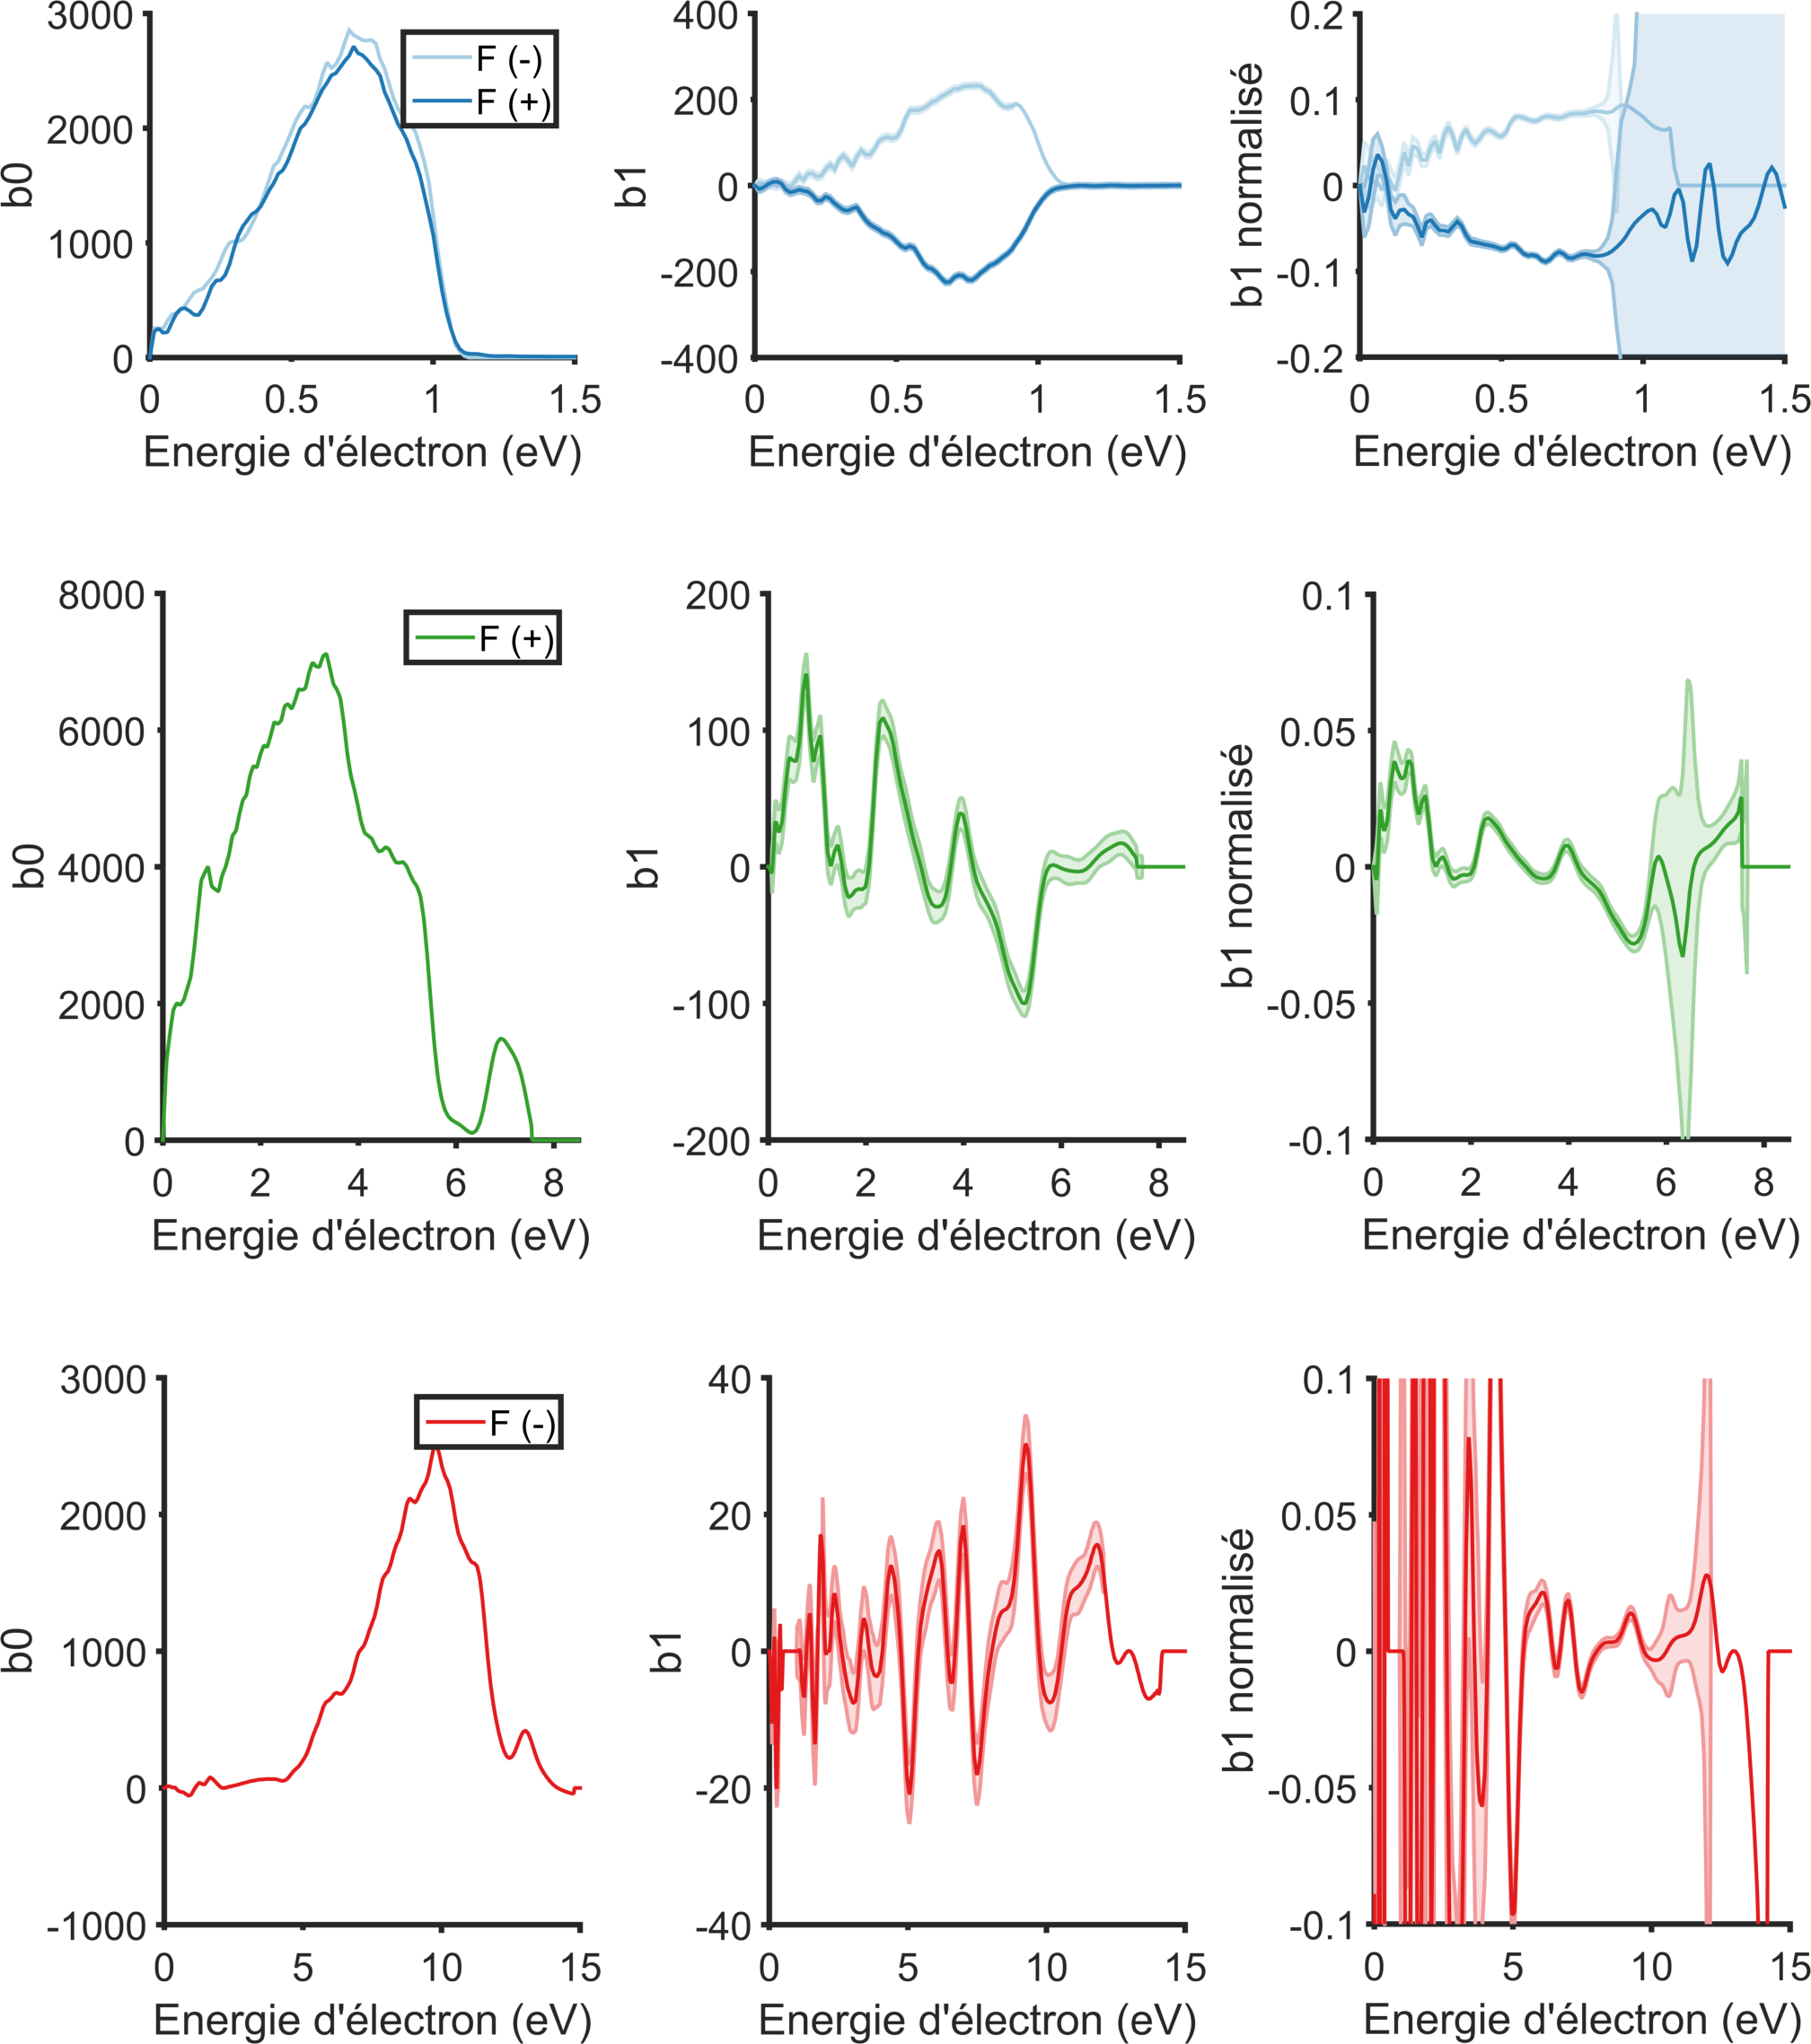
\includegraphics[width=1\columnwidth]{Figures/Soleil/Results_PECD.pdf}%
\caption{Résumé des mesures de PECD réalisées sur la ligne DESIRS. De gauche à droite : $b_0$ (spectre de photoémission), $b_1$, et $b_1$ normalisé par $b_0$. De haut en bas, énergies de photon égales à 9.3 eV, 15.5 eV et 21.7 eV. Pour la première énergie on a tracé la mesure pour les deux énantiomères.}
\label{fig:results_pecd}
\end{figure}

Dans la figure \ref{fig:results_pecd}, on trace $b_0$, $b_1$, et $b_1/b_0$ pour les trois énergies harmoniques et pour un ou deux énantiomère. La polarisation étant ici complètement circulaire, l'utilisation de pBasex est justifiée. Quand on augmente l'énergie de photon, l'énergie maximale de photoélectron observée augmente également. Dans tous les cas, on observe clairement l'ionisation depuis la HOMO, à une énergie égale à $\hbar\omega-I_P^\text{HOMO}$, c'est-à-dire $\simeq \SI{0.7}{eV},\; \SI{6.9}{eV},\text{ et }\SI{13.1}{eV}$ respectivement pour H3, H5 et H7. Pour les énergies de photons plus élevées, la contribution d'orbitales plus basses apparaît. Les énergies de ces orbitales sont de plus en plus proches, et leurs contributions sont sommées dans le $b_1$ observé. $b_1$ est différent pour chacune d'entre elles et peut changer de signe, ce qui explique les profils riches observés dans cette région. Précisons pour terminer qu'à cause de problèmes de calibration en énergie aux hautes énergies de photon, certaines courbes ont été interpolées pour être cohérentes avec potentiels d'ionisation des différentes orbitales publiés dans la littérature \mycite{PowisCPC2008}.
\newpage
\section{Comparaison entre mesures synchrotron et harmoniques}
\subsubsection{Formulation mathématique}
Nous dispose désormais des données synchrotron nécessaires à la caractérisation complète de l'état de polarisation du champ harmonique. Toutefois, nous allons voir que nos mesures harmoniques sont incomplètes. Nous illustrerons ici le principe à suivre mais nous pourrons pas donner de véritable valeurs numériques en l'état.

On considère donc le spectre constitué des 3 première harmoniques du fondamental à 400 nm. Quand il ionise la molécule de fenchone, on observe un spectre de photoémission qui est la somme de la contribution de chaque harmonique :
\[ b^{\text{GHOE}}_0(E) = \sum_{q={3,5,7}} s^{\text{GHOE},q}_0 \times b^{\hbar\omega=E_q}_0(E),\]
où $E_q$ et $s^{\text{GHOE},q}_0$ sont respectivement l'énergie et le $s_0$ (= l'intensité) de la q-ième harmonique.

Les trois mesures synchrotrons donnent quant à elles pour $q=3,5,7$ :
\[ b^{\text{Sync},q}_0(E) =  s^{\text{Sync},q}_0 \times b^{\hbar\omega=E_q}_0(E),\]

Notons les inconnues du problème $a_q = s^{\text{GHOE},q}_0/s^{\text{Sync},q}_0$ pour $q=3,5,7.$ On les obtient par un calcul d'ajustement, par exemple au sens des moindres carrés :
\begin{equation}
\min_{a_q} \sqrt{\int_{E=0}^{E_\text{max}} \left(b^{\text{GHOE}}_0(E)-\sum_{q={3,5,7}} a_q \times b^{\text{Sync},q}_0(E)\right)^2\rmd E}.
\label{eq:minb0}
\end{equation}

La figure \ref{fig:sumb0} présente le profil de $\sum_{q={3,5,7}} b^{\text{Sync},q}_0(E)$, en utilisant les $b_0$ mesurés à la partie précédente (voir figure \ref{fig:results_pecd}). Elle permet de voir les régions dans lesquelles contribuent chaque énergie de photon.

\begin{figure}[!ht]
\centering
\def\svgwidth{0.8\columnwidth}
\import{Figures/Soleil/}{sumPES.pdf_tex}
\caption{Sommes des $b_0$ mesurés au synchrotron à chaque énergie harmonique, en les supposant chacun normalisés et de poids égal.}
\label{fig:sumb0}
\end{figure}

De la même manière, le paramètre dichroïque $b_1$ s'écrit pour les harmoniques :
\[ b^{\text{GHOE}}_1(E) = \sum_{q={3,5,7}} s^q_3 s^{\text{GHOE},q}_0 \times b^{\hbar\omega=E_q}_1(E),\]
et pour les mesures synchrotron, où on considère $s_3=1$ :
\[ b^{\text{Sync},q}_1(E) =  s^{\text{Sync},q}_0 \times b^{\hbar\omega=E_q}_1(E).\]

La quantité à minimiser en fonction des trois inconnues $s_3^3,\;s_3^5,\;s_3^7$ est alors :
\begin{equation}
\min_{s_3^q} \sqrt{\int_{E=0}^{E_\text{max}} \left(b^{\text{GHOE}}_1(E)-\sum_{q={3,5,7}} s^q_3 \times a_q \times b^{\text{Sync},q}_1(E)\right)^2\rmd E}.
\label{eq:minb1}
\end{equation}

En pratique, on minimise à la fois les problèmes \ref{eq:minb0} et \ref{eq:minb1} :
\begin{equation}
\min_{a_q,\;s_3^q} \sqrt{
	\begin{aligned}
	\int_{E=0}^{E_\text{max}}&\alpha_0\left(b^{\text{GHOE}}_0(E)-\sum_{q={3,5,7}} a_q \times b^{\text{Sync},q}_0(E)\right)^2 \\
	&+ \alpha_1\left(b^{\text{GHOE}}_1(E)-\sum_{q={3,5,7}} s^q_3 \times a_q \times b^{\text{Sync},q}_1(E)\right)^2	\rmd E
	\end{aligned}
	}
\label{eq:min_total}
\end{equation}
où $\alpha_0$ et $\alpha_1$ sont les poids relatifs qu'on donne arbitrairement à l'ajustement du $b_0$ et du $b_1$. Cette procédure donnera la valeur optimale de $s_3^3,\;s_3^5$ et $s_3^7$, valeurs inaccessible par des méthodes optiques.

\subsubsection{Première application de la méthode}
Pour les données synchrotron, nous choisissons d'utiliser la mesure sur la fenchone (+) pour H5, et sur la fenchone (-) pour H3 et H7 où on inversera le $b_1$. Ces mesures sont les plus précises du fait d'un très bon niveau de signal, et ne présentent pas de problème de calibration. On prend également soin de corriger les mesures dans la fenchone (-) de l'erreur due à l'excès énantiomérique inférieur à 1.

Pour les données harmoniques, les seules dont nous disposons actuellement sont celles présentées sur la figure \ref{fig:pecdfenchone}. Le problème est qu'elles ont été obtenues par application de l'algorithme pBasex, qui introduit un artefact pour une polarisation non circulaire. On peut toujours étudier le $b_1$ non normalisé par $b_0$ (c'est-à-dire la différence directe entre les deux images), mais la formule \ref{eq:min_total} montre bien la nécessité de connaître $b_0$ pour comparer les deux mesures.

En plus de ce problème d'analyse, ces données ne sont pas parfaites : des zones du détecteurs étaient brûlées (visible sur la figure \ref{fig:pecdfenchone} vers 6 eV), et un bruit de fond n'a pas été correctement soustrait. Nous appliquerons donc le calcul présenté plus haut tout en gardant à l'esprit que les valeurs finales seront incorrectes. 

Le problème \ref{eq:min_total} est résolu au sens des moindres carrés par un algorithme à région de confiance réflectif \mycite{BranchColemanLi1999}. On restreint de plus le domaine d'énergie sur lequel on minimise la fonction, de sorte à ne garder que les pics significatifs. $b_1$ étant le paramètre qui nous intéresse le plus, on choisit des facteurs de pondération $\alpha_1/\alpha_0 = 100$. La figure \ref{fig:results_minim_P} illustre le résultat de l'algorithme, qui converge en quelques dizaines d'itérations, pour la fenchone (+). Les $b_1$ des mesures synchrotrons sont ensuite inversés pour analyser le cas de la fenchone (-), illustré sur la figure \ref{fig:results_minim_M}.

\begin{figure}[!ht]
\centering
\def\svgwidth{0.75\columnwidth}
\import{Figures/Soleil/}{results_minim_P.pdf_tex}
\caption{Détermination des $s_3$ harmoniques par comparaison avec les données synchrotron dans la fenchone (+). En traits pleins bleus, résultats de l'algorithme de minimisation. En pointillés rouges, mesures faites avec la source d'harmoniques d'ordre élevé. Les rectangles verts illustrent le domaine d'énergie où a été effectuée la minimisation. Les valeurs de $s_3$ obtenues sont indiquées.}
\label{fig:results_minim_P}
\end{figure}

\begin{figure}[!ht]
\centering
\def\svgwidth{0.75\columnwidth}
\import{Figures/Soleil/}{results_minim_M.pdf_tex}
\caption{Détermination des $s_3$ harmoniques par comparaison avec les données synchrotron dans la fenchone (-). En traits pleins bleus, résultats de l'algorithme de minimisation. En pointillés rouges, mesures faites avec la source d'harmoniques d'ordre élevé. Les rectangles verts illustrent le domaine d'énergie où a été effectuée la minimisation. Les valeurs de $s_3$ obtenues sont indiquées.}
\label{fig:results_minim_M}
\end{figure}

On note tout d'abord un accord très satisfaisant sur le $b_1$. Ceci démontre la possibilité d'effectuer des mesures précises de PECD avec une source harmonique. L'accord sur le $b_0$ est moins bon, du fait du choix d'un $\alpha_0\ll\alpha_1$. Les valeurs de $s_3$ obtenues sont précisées sur les figures. Précisons encore une fois que ces valeurs ne sont pas correctes à cause des artefacts sur $b_0$ introduits par l'utilisation de pBasex et les défauts expérimentaux. Ce point est bien visible puisque les valeurs de $s_3^5$ et $s_3^7$ diffèrent entre les deux énantiomères, alors que la source est restée la même entre les deux expériences.\par
Toutefois, nous montrons ici la possibilité de réaliser une caractérisation de l'état de polarisation du rayonnement. Pour l'obtenir complètement (ellipticité, dépolarisation, angle de l'ellipse), il faudrait en plus connaître les $s_1$ et $s_2$. Une nouvelle campagne d'expérience est prévue au CELIA Bordeaux, dans laquelle on réalisera les mesures pour l'instant manquantes :


\begin{itemize}
\renewcommand{\labelitemi}{$\bullet$}
\setlength\itemsep{1em}
\item Les données seront cette fois analysées par une autre méthode, en prenant en compte la polarisation elliptique du rayonnement. On obtiendra alors la véritable valeur de $b_0$, permettant de déterminer les $a_q$ correctement.
\item Le détecteur du VMI a été remplacé et ne présente plus de dommage.
\item Un polarimètre a été installé juste après le VMI. Il permet de réaliser des loi de Malus et de mesurer $s_1$, $s_2$, et la borne supérieure $s_3^{\text{max}}$. Il est également adapté à la mesure des paramètres de la troisième harmonique, ce qui n'était pas le cas jusqu'à présent (voir figure \ref{fig:sf6_ell}). Les mesures de PECD et de loi de Malus seront effectuées dans des conditions identiques, ce qui permettra de déterminer $\eta$, $P$, et $\epsilon$. 
\end{itemize}

\chapternonum{Conclusion et perspectives}
Dans cette partie, nous avons d'abord développé une source d'harmoniques d'ordre élevé polarisées elliptiquement. En plus du contrôle du moment angulaire orbital, démontré à la partie précédente, nous contrôlons ici le moment angulaire de spin dans le domaine ultraviolet. En tant qu'objet chiral, la lumière polarisée circulairement est sensible à la chiralité de molécules, ce que nous avons démontré en effectuant des mesures de dichroïsme circulaire de photoélectron. Nous avons réalisé ces mêmes mesures sur un synchrotron, source de lumière parfaitement caractérisée. La comparaison entre les deux montre d'abord que les deux sources donnent des mesures spectroscopiques comparables. Nous avons ensuite étudié la possibilité de caractériser l'état de polarisation de notre source harmonique grâce au PECD.

Au cours de ces études, nous nous sommes intéressés à la GHOE au voisinage de résonances atomiques et moléculaires. Ceci a permis à \mycite{beaulieuArXiv2016} d'expliquer le phénomène de xFID au voisinage du seuil d'ionisation de l'argon. Toujours dans le cadre de notre collaboration avec le CELIA Bordeaux, et en particulier avec Samuel Beaulieu, \'Etienne Bloch, Valérie Blanchet et Yann Mairesse, nous avons poursuivi l'étude de ce phénomène et réalisé des expériences pompe-sonde. Des expériences visant à mesurer des dynamiques transitoires de paquets d'ondes électroniques de Rydberg grâce à cet effet sont en cours au CELIA Bordeaux.

Quant au PECD, nous n'avons présenté qu'ici des mesures \textit{statiques}. Cette grandeur était jusque ici résolue en fréquence dans des expériences réalisées sur synchrotron. Nos travaux permettent de réaliser ces expériences sur une source ultra-brève et d'y ajouter une résolution temporelle. Nous avons commencé une série d'expériences pompe-sonde dans lesquelles on explore les dynamiques électroniques dans des potentiels chiraux. Dans un premier temps, nous nous sommes intéressés au cas plus simple à mettre en œuvre du PECD multi-photonique \mycite{LuxAC2012}. Nos résultats indiquent la possibilité de créer des densités et des courants chiraux, et de les sonder à l'échelle femtoseconde. Ces résultats constituent la première mesure \textit{dynamique} de PECD et feront l'objet d'une prochaine publication. Dans la suite logique de cette démarche, nous préparons des expériences pompe-sondes XUV-Infrarouge, où on pourrait observer des traces similaires au RABBIT (voir section \ref{sec:omabbit}). Nous pourrions ainsi mesurer des délais de photoionisation entre les différents canaux d'ionisation et observer l'effet temporel du potentiel chiral. 


%\partimage[width=1\columnwidth]{Figures/PartImages/FigCh4.png}
\part{Polarisation circulaire, molécules chirales et harmoniques d'ordre élevé}
\label{PA:Spin_HHG}
%\chapter{Génération d'harmoniques d'ordre élevé polarisées elliptiquement}
%\label{CH:Circular_HHG}
%%Dans cette partie nous présenterons comment générer des harmoniques d'ordre élevé portant du moment angulaire de spin, c'est-à-dire ayant une polarisation elliptique. Pour commencer nous donnerons le formalisme utile à la description d'ondes polarisées, puis étudierons le mécanisme de GHOE dans un atome ou une molécule quand le laser de génération est polarisé elliptiquement. Nous verrons que le transfert de moment angulaire n'est pas efficace dans le schéma habituel de GHOE et mentionnerons les solutions existantes, avant d'en démontrer une nouvelle qui utilise une résonance de l'atome ou la molécule de génération.
%
%\section{Formalisme pour la description d'ondes polarisées elliptiquement}
%\label{sec:polardef}
%%Comme on l'a vu dans la partie \ref{sec:circpolar}, le champ électrique d'une onde polarisée elliptiquement décrit une ellipse au cours de sa propagation. Soit $(x,y,z)$ un repère cartésien tel que $z$ soit selon la direction de propagation et $x$ soit selon l'axe majeur de l'ellipse. Un champ elliptique monochromatique s'écrit :
%%\begin{equation}
%%\bm{E}=\begin{pmatrix}
%%E_{x}\cos{(\omega t-kz)}\\
%%E_{y}\sin{(\omega t-kz)}\\
%%0
%%\end{pmatrix}=E_{0}
%%\begin{pmatrix}
%%\cos{(\omega t-kz)}\\
%%\epsilon\sin{(\omega t-kz)}\\
%%0
%%\end{pmatrix},
%%\label{eq:jones}
%%\end{equation}
%%où $\epsilon = E_{y}/E_{x}$ est appelé ellipticité du champ. $\epsilon$ varie de 0 pour une polarisation linéaire à 1 pour une polarisation circulaire.  On a vu que si $\epsilon>0$ (resp. $<0$), l'onde était elliptique gauche (resp. droite) et porte un moment angulaire de spin de $\epsilon\hbar$ (resp. $-\epsilon\hbar$) par photon. 
%%
%%\begin{figure}[!ht]
%%\centering
%%\def\svgwidth{0.6\columnwidth}
%%\import{Figures/Polar/}{polarellipse.pdf_tex}
%%\caption{Définition des différents paramètres de l'ellipse de polarisation.}
%%\label{Fig:polarellipse}
%%\end{figure}
%%Dans un repère où $x$ et $y$ ne sont pas selon les axes de l'ellipse, on note $\eta$ l'angle entre l'axe $x$ et l'axe majeur de l'ellipse (voir figure \ref{Fig:polarellipse}). L'ellipticité est déterminée par le rapport des axes mineurs et majeurs de l'ellipse, $b$ et $a$ : $\epsilon = b/a$. On note $\chi$ l'angle tel que $\tan\chi = \epsilon = b/a$. Comme les amplitudes du champ selon les axes de l'ellipse sont déphasées de $\pi/2$, $a$ et $b$ peuvent être vus comme les parties réelle et imaginaire d'un vecteur de polarisation complexe et unitaire $\bm{\Pi}$. Le champ s'écrit alors :
%%\[\bm{E} = E_x \bm{e_x} + E_y \bm{e_y} = E_0(\Pi_x \bm{e_x} + \Pi_y \bm{e_y}).\] 
%%Il sera utile d'utiliser les \textit{paramètres de Stokes}, définis comme :
%%\begin{align}
%%s_0 &= E_xE_x^*+E_yE_y^* =E_0^2,\nonumber\\
%%s_1 &= E_xE_x^*-E_yE_y^* =E_0^2\cos 2\chi\cos 2\eta ,\nonumber\\
%%s_2 &= -\left(E_xE_y^*+E_yE_x^*\right)=E_0^2\cos 2\chi\sin 2\eta,\nonumber\\
%%s_3 &= -\rmi\left(E_xE_y^*-E_yE_x^*\right)=E_0^2\sin 2\chi,	
%%\label{eq:stokes1}
%%\end{align}
%%où nous avons utilisés les conventions de signe de \mycite{barron}. Pour une onde monochromatique, ces paramètres donnent $E_0$, $\chi$ et $\eta$, ou de manière équivalente, l'intensité $I_0$, l'ellipticité $\epsilon$ et $\eta$. Ils caractérisent donc totalement le champ électrique. Il ne sont pas indépendants : on a $s_0^2 = s_1^2+s_2^2+s_3^2$. 
%%
%%En pratique, les ondes utilisées ne sont que \textit{quasi}-monochromatiques. Elles possèdent une largeur spectrale $\Delta\omega$ non nulle, à l'intérieur de laquelle les différentes composantes fréquentielles ne possèdent pas forcément les mêmes polarisations et phases. Le vecteur du champ électrique apparent, somme de toutes les composantes fréquentielles, ne décrit alors plus une ellipse. Dans le cas extrême, il ne présente aucune direction préférentielle : on parle alors de lumière \textit{non polarisée}. De manière générale, le vecteur du champ électrique n'évolue pas complètement régulièrement ou irrégulièrement, la lumière est alors dite \textit{partiellement} polarisée.
%%
%%Dans une expérience, le temps d'observation est en général long comparé à $1/\Delta\omega$. Les paramètres de Stokes doivent donc être définis à partir de la moyenne temporelle des quantités définies en \ref{eq:stokes1}. Ces expressions font intervenir les produits des composantes de $\bm{\Pi}$. Pour une lumière complètement polarisée,
%%\[\overline{\Pi_x \Pi^*_y} = \Pi_x \Pi^*_y,\]
%%et on retrouve les mêmes propriétés que pour une onde monochromatique. \`{A} l'autre extrême, si la lumière est non polarisée, toutes les orientations de $\bm{\Pi}$ sont équiprobables :
%%\[\overline{\Pi_x \Pi^*_y} = 0.\]
%%Les paramètres de Stokes deviennent donc $S_0 = E_0^2$ et $s_1^2 = s_2^2 = s_3^2 = 0$. Dans le cas d'une lumière partiellement polarisée, on obtient donc $s_0^2 > s_1^2+s_2^2+s_3^2$. On introduit alors le degré de polarisation de la lumière $P$, défini comme 
%%\[P = \frac{\sqrt{s_1^2+s_2^2+s_3^2}}{s_0}.\] $P$ varie entre $0$ pour une lumière non polarisée et $1$ pour une polarisation complète. Une lumière partiellement polarisée peut être séparée entre une composante non polarisée et une complètement polarisée, dont les paramètres d'ellipse sont bien définis. On les retrouve à partir des paramètres de Stokes :
%%\begin{align}
%%s_0 &= E_0^2,\nonumber\\
%%s_1 &= PE_0^2\cos 2\chi\cos 2\eta ,\nonumber\\
%%s_2 &= PE_0^2\cos 2\chi\sin 2\eta,\nonumber\\
%%s_3 &= PE_0^2\sin 2\chi,	
%%\label{eq:stokes2}
%%\end{align}
%%Les paramètres de l'onde s'obtiennent en inversant \ref{eq:stokes2} :
%%\begin{align}
%%E_0^2 &= s_0,\nonumber\\
%%\eta &= \frac{1}{2} \arctan\left(\frac{s_2}{s_1}\right),\nonumber\\
%%\chi &= \frac{1}{2} \arctan\left(\frac{s_3}{\sqrt{s_1^2+s_2^2}}\right),\nonumber\\
%%P &= \sqrt{s_1^2+s_2^2+s_3^2}/s_0
%%\label{eq:stokes2inv}
%%\end{align}
%%
%%L'onde est maintenant complètement décrite par $E_0$, $\chi$, $\eta$ et $P$. Cette description est similaire à celle d'un système en mécanique quantique. En effet, une description vectorielle telle que l'expression \ref{eq:jones} (appelé vecteur de Jones) ne peut décrire qu'une polarisation complète. Une polarisation partielle est une superposition incohérente de polarisations complètes, bien décrite par le formalisme de Stokes. De la même manière, un état quantique pur est décrit par une fonction d'onde, analogue du vecteur de Jones. Un état quantique mixte, qui est une superposition d'états purs, doit être décrit par une matrice densité, analogue du vecteur de Stokes. Cette analogie n'est pas fortuite : la lumière provient généralement d'une transition entre deux états quantiques, par exemple d'un atome. Les propriétés de polarisation de la lumière découlent alors de la cohérence entre ces états, comme décrit en détail dans \mycite{fano1957}. 
%%
%%Pour terminer, notons qu'en plus d'une inhomogénéité temporelle, la polarisation partielle de la lumière peut également découler d'une inhomogénéité spatiale : si les paramètres de l'ellipse varient avec la coordonnée transverse et que l'expérience moyenne spatialement ces différentes contributions, on aura $P<1$.
%%
%\section{GHOE à partir d'un faisceau infrarouge polarisé elliptiquement}
%\label{sec:ghoepolar}
%%Dans la partie précédente, nous avons démontré qu'en donnant du moment angulaire orbital à l'infrarouge de génération, il était transmis au rayonnement harmonique. Ce principe devrait s'appliquer au moment angulaire de spin, qui doit être conservé dans le processus. 
%
%\subsection{Résultats de la littérature}
%%\mycite{budilPRA1993} ont réalisé la première expérience à ce sujet. Ils ont généré les harmoniques d'ordre élevé d'un laser Cr:LiSAF et mesuré l'intensité de chaque harmonique en fonction de l'ellipticité de l'infrarouge. Le résultat pour le néon est présenté sur la figure \ref{Fig:budil}.
%%\begin{figure}[!ht]
%%\centering
%%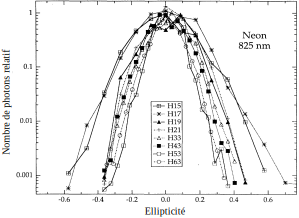
\includegraphics[width=0.6\columnwidth]{Figures/Polar/Intensity_f_ellipticity_budil}%
%%\caption{Intensité normalisée des harmoniques produites dans le néon en fonction de l'ellipticité. Tiré de \mycite{budilPRA1993}}%
%%\label{Fig:budil}%
%%\end{figure}
%%
%%On observe une décroissance de l'intensité harmonique en fonction de l'ellipticité. Cet effet est marqué : on perd environ un ordre de grandeur en intensité quand $|\epsilon_{IR}| = 0.2$. On remarque également que cette décroissance est de plus en plus piquée lorsque l'ordre harmonique augmente.
%%
%%\'{E}tudions ensuite les résultats de \mycite{AntoinePRA1997}. Les auteurs se sont cette fois intéressés à l'état de polarisation du rayonnement harmonique en fonction de l'ellipticité de l'infrarouge. Ces expériences ont été réalisées sur une version antérieure du système laser que nous avons utilisé dans la partie III. Pour caractériser le rayonnement, les auteurs mesurent des \textit{lois de Malus}, méthode optique qui sera présentée plus loin (section \ref{sec:resonant_argon_exp}). Comme on le verra, cette technique est incapable de mesurer le degré de polarisation $P$. Elle ne donne qu'une borne supérieure sur l'ellipticité, atteinte uniquement lorsque la lumière est complètement polarisée. Ce point est crucial dans le cas de la GHOE : comme expliqué dans la partie \ref{sec:phase_spatiale} le dipôle de chaque ordre harmonique dépend de l'intensité infrarouge. Le champ émis sera donc non homogène en polarisation spatialement et temporellement, donc nécessairement partiellement polarisé.
%%
%%La figure \ref{fig:antoinepra} présente quelques résultats extraits de \mycite{AntoinePRA1997}. On y voit l'évolution de l'ellipticité des harmoniques et de l'angle d'orientation de l'ellipse $\eta$, pris par rapport à un axe de référence fixe. L'ellipticité mesurée n'étant qu'une borne supérieure de l'ellipticité vraie, on la note $\epsilon^{max}_q$. La figure \ref{fig:antoinepra} inclut un résultat numérique qui donne lui accès à $P$ et donne une idée de la quantité de lumière non-polarisée.
%%
%%\begin{figure}[!ht]
%%\centering
%%\def\svgwidth{\columnwidth}
%%\import{Figures/Polar/}{antoinePRA.pdf_tex}
%%\caption{\`{A} gauche, mesure de l'ellipticité des harmoniques 17 et 23 générées dans l'argon par un champ infrarouge elliptique. Carrés rouges : mesures expérimentales de $\epsilon^{max}_q$ par loi de Malus. Comme expliqué plus haut, ce n'est qu'une borne supérieure sur la vraie valeur de l'ellipticité. En traits rouges, même quantité obtenue par le calcul. En pointillés noirs, véritable ellipticité obtenue par le calcul. En traits-pointillés verts, degré de polarisation obtenu par le calcul. \`{A} droite, mesure de l'angle de rotation de l'ellipse (carrés rouges) et même quantité obtenue par le calcul (traits rouges). Adapté de \mycite{AntoinePRA1997}.}
%%\label{fig:antoinepra}
%%\end{figure}
%%
%%On fait les observations suivantes :
%%\begin{itemize}
%%\renewcommand{\labelitemi}{$\bullet$}
%%\setlength\itemsep{1em}
%%\item $\epsilon^{max}_q$ est une fonction croissante de $\epsilon_{IR}$ sur l'intervalle parcouru.
%%\item $|\epsilon^{max}_q|$ augmente plus rapidement avec $|\epsilon_{IR}|$ pour l'harmonique plus basse.
%%\item Le rayonnement est de moins en moins polarisé à mesure que $|\epsilon_{IR}|$ augmente. Cet effet est plus fort pour l'harmonique basse.
%%\item Cette diminution de $P$ s'accompagne d'une ellipticité vraie plus faible. Pour l'harmonique la plus basse, l'ellipticité vraie est presque \textit{deux fois inférieure} à l'ellipticité mesurée.
%%\item $\eta$ est également une fonction croissante de $\epsilon_{IR}$.
%%\item $\eta$ augmente plus rapidement pour l'harmonique basse.
%%\end{itemize}
%%\vspace{\baselineskip}
%%Ces deux travaux démontrent deux résultats généraux. En premier lieu, on voit que l'ellipticité de l'infrarouge est bien transférée au champ harmonique. Toutefois, l'ellipticité harmonique semble toujours rester inférieure à celle du laser générateur. Deuxièmement, le rendement harmonique décroît exponentiellement avec l'ellipticité de l'infrarouge. Nous concluons donc qu'il est très difficile d'obtenir un rayonnement ultraviolet d'ellipticité significative tout en gardant un niveau de signal suffisant. Dans la section suivante, nous expliquons les effets physiques à l'origine de ces propriétés.
%
%\subsection{Description théorique de la GHOE en polarisation elliptique}
%%Dans le modèle à trois étapes (voir section \ref{sec:threestep}), la polarisation du champ intervient dans le calcul de la trajectoire électronique dans le continuum. On note $(x,y)$ la position dans le plan transverse de l'électron, que l'on considère classiquement. Sa trajectoire dans un champ complètement polarisé est donnée par :
%%\[\left\{
%%\begin{array}{l}
  %%\ddot{x}(t) = -\frac{qE_0}{m}\cos\omega t \\
  %%\ddot{y}(t) = -\epsilon\frac{qE_0}{m}\sin\omega t,
%%\end{array}
%%\right.\]
%%avec $q$ et $m$ la charge et la masse de l'électron, et $\epsilon$ et $\omega$ l'ellipticité et la fréquence angulaire du champ. L'équation selon $x$ se résoud exactement de la même façon que pour une polarisation linéaire : on suppose $x(t_i) = \dot{x}(t_i) = 0$, où $t_i$ est le temps d'ionisation, et pour chaque $t_i$, on obtient l'instant de recombinaison $t_r$.
%%
%%Selon la dimension $y$, l'électron doit bien sûr être émis au niveau du noyau : $y(t_i) = 0$. Cependant, si on suppose que $\dot{y}(t_i) = 0$, l'équation $y(t_r) = 0$ n'a pas de solution : l'électron 'rate' l'atome et ne peut pas recombiner, comme illustré sur la figure \ref{fig:ellgruson}.
%%
%%\begin{figure}[!ht]
%%\centering
%%\def\svgwidth{0.7\columnwidth}
%%\import{Figures/Polar/}{trajClassique.pdf_tex}
%%\caption{Trajectoire classique d'un électron dans un champ électrique elliptique, en supposant $x(t_i) = \dot{x}(t_i) = 0$ et $y(t_i) = \dot{y}(t_i) = 0$. La longueur d'onde est 800 nm et l'éclairement est $\SI{2e14}{W/cm^2}$. La polarisation du champ infrarouge est schématisée en gris. Adapté de \mycite{gruson}.}
%%\label{fig:ellgruson}
%%\end{figure}
%%
%%Classiquement, la génération d'harmonique en polarisation elliptique est donc impossible. En vérité, le déplacement et la vitesse de l'électron selon l'axe $y$ sont trop faibles pour utiliser une description classique. Si on décrit cette dimension quantiquement, on a un paquet d'onde électronique émis lors de l'ionisation tunnel. Ce paquet d'onde est localisé spatialement autour de l'atome, sur une longueur $\Delta y$ dépendant de l'orbitale en jeu. Le moment cinétique selon $y$ est donc lui aussi confiné à une largeur $\Delta p_y$. La distribution de $p_y$ est centrée sur y=0 à $t=0$ et peut maintenant contenir des valeurs non nulles. \mycite{strelkov2006} démontre que pour avoir recombinaison, le moment cinétique initial doit valoir $p_y(t=0) = -\bar{y}/\tau$, où $\bar{y}$ est la quantité représentée sur la figure \ref{fig:ellgruson}, et $\tau$ le temps d'excursion total de l'électron. Ceci permet d'expliquer simplement le résultat de \mycite{budilPRA1993} présenté plus haut : si $\epsilon_{IR}$ augmente, $\bar{y}$ augmente également. Il faut donc un moment cinétique initial plus important pour avoir recombinaison, ce qui est moins probable puisque la distribution de $p_y(t=0)$ est centrée en y=0. Ceci explique la diminution du rendement harmonique avec l'ellipticité de l'infrarouge.
%%
%%Pour comprendre qualitativement les résultats de \mycite{AntoinePRA1997}, on trace les trajectoires classiques de l'électron, cette fois avec la condition initiale $p_y(t=0) = -\bar{y}/\tau$ et avec les deux trajectoires quantiques.
%%
%%\begin{figure}[!ht]
%%\centering
%%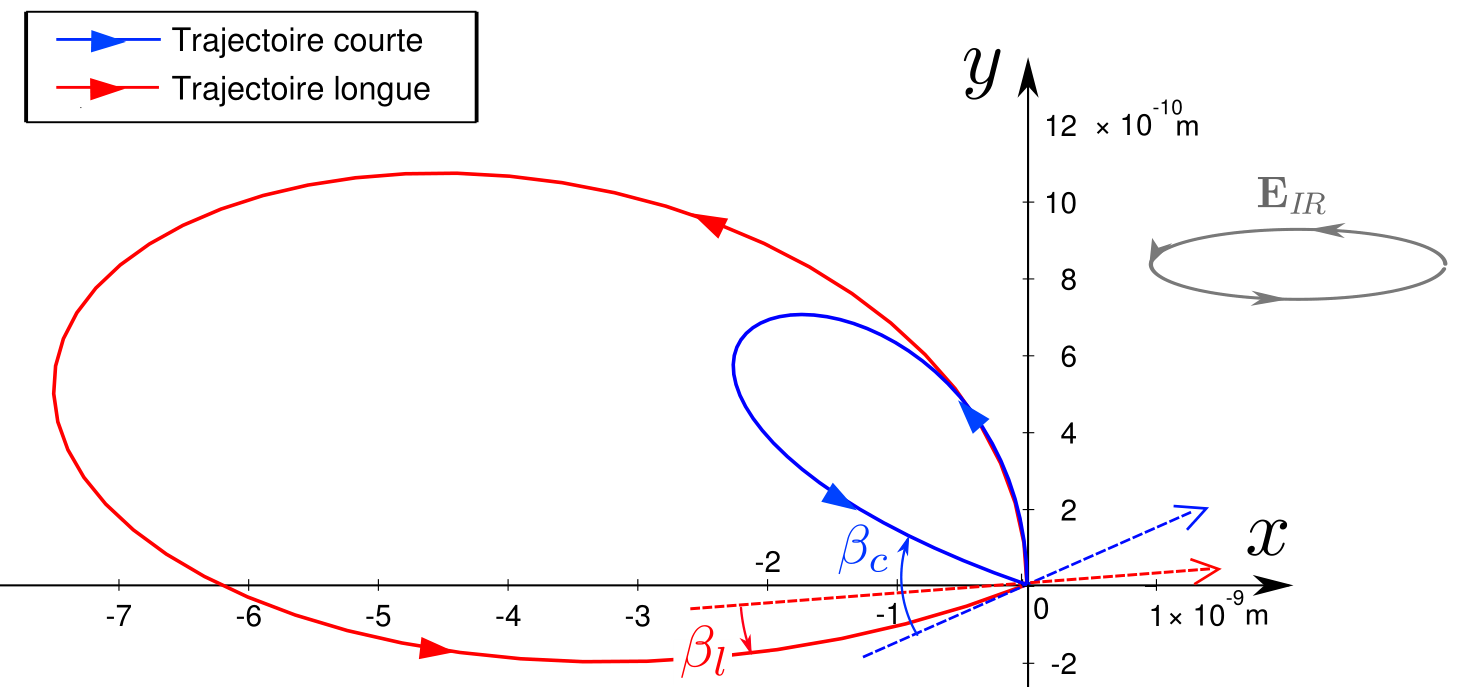
\includegraphics[width=0.9\columnwidth]{Figures/Polar/higuet.png}%
%%\caption{Trajectoires électroniques correspondant à l’harmonique 111 d'un laser à 1800 nm, pour un éclairement de $\SI{1e14}{W/cm^2}$ et une ellipticité de 0.2 (champ représenté en gris).
%%En ligne pointillée, la direction du champ à l’instant d’ionisation. On notera la différence entre les échelles
%%des axes $x$ et $y$. Tiré de \mycite{higuet}}
%%\label{fig:ellhiguet}%
%%\end{figure}
%%
%%La figure \ref{fig:ellhiguet}, tirée de \mycite{higuet}, n'est pas directement comparable à la figure \ref{fig:ellgruson}, le calcul ayant été réalisé à une longueur d'onde plus élevée. Une longueur d'onde plus grande conduit à des trajectoires électroniques plus longues et à des effets plus marqués qu'à 800 nm.
%%On observe toutefois un effet intéressant : l'électron recombine sur l'atome avec un angle variable $\beta_{c/l}$ (pour trajectoire courte/longue). Cette angle est responsable de la rotation d'angle $\eta$ de l'ellipse harmonique. En effet, pour une orbitale de symétrie sphérique, l'axe principal de l'ellipse de polarisation du rayonnement harmonique est dirigé selon la direction de recollision de l'électron à la recombinaison \mycite{strelkov2006}. L'ellipse harmonique est donc tournée d'un angle $\beta_{c/l}\approx\eta$, qui dépend de l'ordre harmonique et de la trajectoire considérée. On remarque que $\beta_c$ et $\beta_l$ sont de signes différents, la dépendance de $\eta$ est donc de signe opposé pour la trajectoire longue. Ceci peut être mesuré expérimentalement (voir e.g. la figure 3.11 de \mycite{higuet}).\par
%%Enfin, cet angle explique également que le rayonnement harmonique soit elliptique. L'argument donné par \mycite{Strelkov2011} est le suivant : on considère un état lié $\psi_0(x,y,z) = \psi(x)\psi(y)\psi(z)$ et un paquet d'onde électronique. Ce paquet se déplace principalement dans la direction $x$ et possède une amplitude dans les deux autres dimensions : $\chi(x,y,z) = f(y,z)\exp(\rmi p_x x)$. Comme on l'a vu, l'amplitude $f(y,z)$ est initialement centrée en $y=0$ puis se décale selon $y$ au cours de la propagation. \`{A} la recombinaison, on peut faire un développement de Taylor de $f$ : $f(y,z) = f_0 + f_1 y$, où $f_1$ est relié à l'angle de recombinaison. Le moment dipolaire du système vaut 
%%\[\bm{d} = \int{\psi_0^* \bm{r} \chi \rmd\bm{r}} + \text{c.c.}\]
%%On obtient donc ses composantes cartésiennes :
%%\[d_x \propto f_0 \text{  et  } d_y \propto \rmi f_1.\]
%%On excite donc un dipôle dans les deux directions transverses, et leurs oscillations sont décalées de $\pi/2$. Le signal émis est donc polarisé elliptiquement.
%
%\section{Méthodes existantes de génération d'harmoniques elliptiques}
%%Dans la partie précédente, nous avons expliqué le mécanisme de GHOE en polarisation elliptique et vu que le processus ne permettait pas un transfert direct et efficace de l'ellipticité de l'infrarouge vers l'ultraviolet. Nous présentons ici trois méthodes existantes pour circonvenir à ce problème. 
%
%\subsection{Réflexion sur des surfaces métalliques}
%\label{sec:metalsurface}
%%L'idée est ici de générer des harmoniques polarisée linéairement puis d'utiliser un dispositif similaire à une lame quart d'onde. Dans ces gammes spectrales, il est impossible de réaliser une lame quart-d'onde conventionnelle, mais on peut obtenir le même effet à partir de plusieurs surfaces métalliques. \par
%%On appelle plan d'incidence le plan formé par le vecteur d'onde du champ incident et le vecteur normal à la surface. Il est alors courant d'appeler $p$ la composante du champ \textit{parallèle} à ce plan et $s$ la composante perpendiculaire (\textit{senkrecht} en allemand). Selon le métal utilisé, ces deux composantes ne sont pas réfléchies également : la surface métallique présente une réflectivité selon chaque dimension, habituellement notées $R_p$ et $R_s$. De plus, elle introduit un déphasage entre ces deux composantes. Il est ainsi possible d'introduire un déphasage de $\pi/2$ en choisissant une bonne combinaison de miroirs. \mycite{VodungboOE2011} ont développé un dispositif à 4 miroirs de Mo/$\text{B}_\text{4}$C qui permettent d'obtenir les harmoniques 31 à 45 avec une ellipticité variant de 1 à 0.61. Ces caractéristiques sont très intéressantes, malgré un inconvénient majeur : la transmission du dispositif varie entre 2.6 et 3.7 \% sur la plage considérée. Ce type de dispositif a continué à être amélioré, \mycite{WillemsPRB2015} reportent par exemple une transmission de 10-30\% et une ellipticité de $\approx 0.8$ entre 45 et 70 eV.\par
%%
%%Ces dispositifs sont assez difficiles à implémenter, ce qui couplé à leur faible transmission explique qu'ils ne soient pas très répandus aujourd'hui. 
%
%\subsection{Génération dans des molécules alignées}
%%Considérons la GHOE avec un faisceau polarisé linéairement, cette fois dans un gaz de molécules diatomiques. Au niveau microscopique, l'orientation de l'axe de la molécule par rapport à la polarisation du laser joue un rôle crucial : l'angle de recombinaison de l'électron par rapport à cet axe modifie l'émission, exactement comme le champ elliptique représenté sur la figure \ref{fig:ellhiguet}. L'électron peut donc exciter les deux composantes du dipôle. L'interprétation est toutefois plus compliquée, puisque l'ellipticité obtenue dépend de la symétrie de ou des orbitales ionisées, de leur phases relatives ou encore de l'intensité de génération (voir \mycite{MairessePRL2010}). \par
%%\`{A} l'échelle macroscopique, toutes les orientations de molécules par rapport au laser sont équiprobables. On a donc un effet de moyenne, qui donne un rayonnement harmonique macroscopique polarisé linéairement. Il faut donc \textit{aligner} les molécules. Une technique courante est l'alignement impulsionnel, qui utilise une pré-impulsion quelques secondes avant l'impulsion de génération \mycite{RoscaPRL2001}. La figure \ref{fig:n2ell} présente deux exemples de résultats obtenus avec $\text{N}_\text{2}$, tirés de \mycite{ZhouPRL2009} et \mycite{MairessePRL2010}. Dans les deux cas, on observe un maximum d'ellipticité pour l'harmonique 23 et pour un angle d'alignement d'environ 60\degres.
%%
%%\begin{figure}[!ht]
%%\centering
%%\def\svgwidth{1\columnwidth}
%%\import{Figures/Polar/}{n2ell.pdf_tex}
%%\caption{Mesures d'ellipticité en fonction de l'ordre harmonique et de l'angle d'alignement des molécules de $\text{N}_\text{2}$ par rapport à la polarisation du laser. \`{A} gauche, résultat tiré de \mycite{ZhouPRL2009}, où I = $\SI{2e14}{W/cm^2}$. \`{A} droite, résultat tiré de \mycite{MairessePRL2010}, où I = $\SI{8e13}{W/cm^2}$. Les ellipticités mesurées ici sont des bornes supérieures et non pas la vraie valeur.}
%%\label{fig:n2ell}
%%\end{figure}
%%
%%Ce résultat s'explique en fait par la présence de plusieurs canaux d'ionisation et est donc très intéressant du point de vue de la spectroscopie harmonique. Il est toutefois assez peu flexible et nécessite d'aligner des molécules, et fournit une ellipticité modeste. De plus, l'utilisation d'une impulsion d'alignement a tendance à créer davantage d'inhomogénéités spatiales et temporelles, ce qui produit un rayonnement peu polarisé. Cette question est étudiée en détail expérimentalement dans la thèse de Vincent Gruson \mycite{gruson}.
%%
%\subsection{Manipulation de la trajectoire électronique par un champ bicolore}
%%Terminons par la méthode la plus récente, qui est peut-être la plus intuitive. Le principe est ici de contrôler optiquement la trajectoire électronique de sorte à ce que la recombinaison soit possible quelque soit l'ellipticité infrarouge. Une solution à ce problème a été initialement donnée par \mycite{EichmannPRA1995}. En utilisant un champ à deux couleurs d’ellipticités opposées et de deux longueurs d'onde commensurables, par exemple 400 et 800 nm, la GHOE est possible. L'expérience réalisée par \mycite{FleischerNP2014} montre que la génération est efficace dans ces conditions, et permet de générer des harmoniques paires et impaires d'ellipticité $|\epsilon^{max}_q|\approx 1$. \mycite{KfirNP2015} a mesuré l'hélicité (le signe de $\epsilon$) et montré que les ordres harmoniques étaient polarisés ainsi:
%%\[\left\{
%%\begin{aligned}
  %%\text{Si }q&=3m-1,\quad &\epsilon_q \approx \pm 1 \\
	%%&=3m+1, &\epsilon_q \approx \mp 1 \\
	%%&=3m, &\text{l'harmonique n'est pas générée},
%%\end{aligned}
%%\right.\]
%%où $\pm$ dépend de l'hélicité des champs générateurs. Cette méthode est très intéressante car elle produit un rayonnement fortement polarisé et intense. Elle a été utilisée avec succès par \mycite{KfirNP2015} pour réaliser des mesures de dichroïsme circulaire magnétique dans le cobalt, un effet voisin de ceux dont il sera question au chapitre \ref{sec:PECD}. Cette méthode est ainsi particulièrement adaptée à la spectroscopie de la phase solide.\par
%%La réponse d'une molécule est quant à elle plus difficile à interpréter. En effet, un grand nombre de degrés de liberté et différents canaux d'ionisation contribuent au spectre total, et il n'est jamais facile d'identifier chacune de ces contributions. 
%%On préférera donc avoir un rayonnement très simple, de sorte à exciter le moins d'effets possibles et de pouvoir les identifier. La technique présentée ici fournit un spectre harmonique dense fait d'harmoniques paires et impaires d'hélicité en alternance, ce qui est à l'opposé des besoins de la spectroscopie moléculaire.
%
%\section{Une image photonique de la GHOE en polarisation elliptique}
%%Les travaux de \mycite{FleischerNP2014} que nous venons de mentionner ont suscité de nombreuses questions sur la conservation du moment angulaire de spin dans la GHOE. Avant ces travaux, la conservation du spin n'avait été étudiée ni théoriquement, ni expérimentalement.
%%
%%Jusqu'à présent, nous avons utilisé une description macroscopique du champ électromagnétique. \`A l'étape de recombinaison de la GHOE, l'électron recombine sur l'état fondamental de l'atome. Le processus de GHOE peut être vu comme un processus \textit{paramétrique} dans lequel l'état initial et final sont les mêmes. On considère alors que chaque photon harmonique est issu de l'absorption et/ou de l'émission d'un certain nombre de photons du fondamental. Si la GHOE est effectivement un processus paramétrique, elle doit conserver l'énergie, la quantité de mouvement et les moments angulaires orbitaux et de spin. Nous avons pu observer la conservation des trois premières quantités au cours de cette thèse, et nous intéressons ici à la quatrième.
%%
%%\mycite{FleischerNP2014} ont proposé un modèle simple prédisant le MAS de chaque harmonique dans leur dispositif à deux couleurs, en supposant la conservation du MAS. De manière surprenante, ils observèrent de très larges déviations à ce modèle et proposèrent deux mécanismes pour les expliquer : (1) l'électron ionisé emporte avec lui un moment angulaire de spin non nul, ce qui remet en question le fait que la GHOE soit un processus paramétrique, et (2) les différentes harmoniques sont émises de façon corrélées, ce qui empêche de considérer le moment angulaire de spin d'une harmonique seule.\par
%%\mycite{PisantyPRA2014} proposa ensuite un modèle différent, qui montra que les données de \mycite{FleischerNP2014} étaient cohérentes avec la conservation du MAS sans avoir à utiliser de tels arguments. Nous reprenons sa démarche pour expliquer le cas plus simple de la génération à un seul faisceau polarisé elliptiquement, déjà décrit macroscopiquement dans la partie \ref{sec:ghoepolar}, mais cette fois avec une image photonique.
%%
%%On considère un champ d'ellipticité $\epsilon_0$ arbitraire. On décompose ce champ sur la base des ondes circulaires droites et gauches :
%%\begin{equation}
%%\bm{E} = \frac{E_0 e^{-\rmi\omega t}}{2\sqrt{2}}\left(\frac{1+\epsilon_0}{\sqrt{1+\epsilon_0^2}}\bm{e}_R+\frac{1-\epsilon_0}{\sqrt{1+\epsilon_0^2}}\bm{e}_L\right)+\text{c.c.},
%%\label{eq:Eell_RL}
%%\end{equation}
%%où $\bm{e}_{R/L}=(\bm{e}_x\pm\rmi\bm{e}_y)/\sqrt{2}$ sont les vecteurs unitaires complexes des polarisations circulaires droites et gauches.
%%
%%Les composantes R et L du champ sont alors considérées séparément : on note $n_R$ et $n_L$ le nombre de photons respectif impliqués dans le processus. On note $q$ l'ordre harmonique, et la conservation de l'énergie s'écrit :
%%\[ q\hbar\omega = n_R\hbar\omega+n_L\hbar\omega, \]
%%soit $q = n_R + n_L$, ce qui est consistant avec la conservation de la parité car le nombre de photon absorbé est impair. On a donc un grand nombre de paires $(n_R,n_L)$ qui contribuent à l'émission de chaque harmonique $q$. On peut restreindre ces paires en écrivant la conservation du moment angulaire de spin pour chacune d'entre elles. En notant $s$ le MAS, on a :
%%\[s_{(n_R,n_L)} = n_R s_R + n_L s_L = n_R - n_L.\]
%%Le MAS d'un photon ne peut prendre que deux valeurs : $s_{(n_R,n_L)}=\pm1$, ce qui restreint les canaux possibles à 2 :
%%\[n_R = \frac{q+1}{2},\; n_L = \frac{q-1}{2}\quad\text{ou}\quad n_R = \frac{q-1}{2},\; n_L = \frac{q+1}{2}.\]
%%
%%Ces deux canaux n'ont pas la même amplitude. Par simplicité, on suppose que l'amplitude d'un processus à n-photons évolue comme la $\text{n}^{i\`{e}me}$ puissance du champ fondamental. Cette approximation est un développement perturbatif à l'ordre le plus bas, qui a de nombreuses limitations pour la description de la GHOE, comme l'absence de plateau. On verra qu'elle permet toutefois de comprendre les comportements observés. Dans cette approximation, l'expression \ref{eq:Eell_RL} donne l'amplitude de chaque canal :
%%\[ E_{(n_R,n_L)} \propto \left(\frac{1+\epsilon_0}{\sqrt{1+\epsilon_0^2}}\right)^{n_R}\left(\frac{1-\epsilon_0}{\sqrt{1+\epsilon_0^2}}\right)^{n_L}\]
%%donc son intensité est :
%%\[ I_{(n_R,n_L)} \propto \left(\frac{1+\epsilon_0}{\sqrt{1+\epsilon_0^2}}\right)^{2n_R}\left(\frac{1-\epsilon_0}{\sqrt{1+\epsilon_0^2}}\right)^{2n_L}\]
%%
%%On somme alors les deux canaux pondérés par $I_{(n_R,n_L)}$ pour obtenir la valeur moyenne du MAS de chaque harmonique :
%%\begin{align}
%%<s_q> &= \frac{I_{(\frac{q+1}{2},\frac{q-1}{2})} s_{(\frac{q+1}{2},\frac{q-1}{2})}+I_{(\frac{q-1}{2},\frac{q+1}{2})} s_{(\frac{q-1}{2},\frac{q+1}{2})}}{I_{(\frac{q+1}{2},\frac{q-1}{2})}+I_{(\frac{q-1}{2},\frac{q+1}{2})}}\nonumber\\
%%&= \frac{\left(\frac{1+\epsilon_0}{\sqrt{1+\epsilon_0^2}}\right)^{q+1}\left(\frac{1-\epsilon_0}{\sqrt{1+\epsilon_0^2}}\right)^{q-1}
%%-
%%\left(\frac{1+\epsilon_0}{\sqrt{1+\epsilon_0^2}}\right)^{q-1}\left(\frac{1-\epsilon_0}{\sqrt{1+\epsilon_0^2}}\right)^{q+1}
%%}{
%%\left(\frac{1+\epsilon_0}{\sqrt{1+\epsilon_0^2}}\right)^{q+1}\left(\frac{1-\epsilon_0}{\sqrt{1+\epsilon_0^2}}\right)^{q-1}
%%+
%%\left(\frac{1+\epsilon_0}{\sqrt{1+\epsilon_0^2}}\right)^{q-1}\left(\frac{1-\epsilon_0}{\sqrt{1+\epsilon_0^2}}\right)^{q+1}
%%}\nonumber\\
%%&= \frac{2\epsilon_0}{1+\epsilon_0^2}
%%\label{eq:mas_q}
%%\end{align}
%%
%%On obtient également l'évolution de l'intensité harmonique en fonction de l'ellipticité comme la somme de l'intensité des deux canaux :
%%\begin{align}
%%I_q &= \frac{1}{2}\left[\left(\frac{1+\epsilon_0}{\sqrt{1+\epsilon_0^2}}\right)^{q+1}\left(\frac{1-\epsilon_0}{\sqrt{1+\epsilon_0^2}}\right)^{q-1}+\left(\frac{1+\epsilon_0}{\sqrt{1+\epsilon_0^2}}\right)^{q-1}\left(\frac{1-\epsilon_0}{\sqrt{1+\epsilon_0^2}}\right)^{q+1}\right]\nonumber\\
%%&= \left(\frac{(1+\epsilon_0)(1-\epsilon_0)}{\sqrt{1+\epsilon_0^2}}\right)^{q}\times\frac{1+\epsilon_0^2}{1-\epsilon_0^2}
%%\label{eq:I_q}
%%\end{align}
%%
%%Ces deux quantités sont tracées sur la figure \ref{fig:mas_photon}. Ce modèle simple reproduit qualitativement les mesures de \mycite{AntoinePRA1997} et \mycite{budilPRA1993} (figures \ref{fig:antoinepra} et \ref{Fig:budil}) : l'ellipticité harmonique augmente avec l'ellipticité du fondamental, et l'efficacité du processus décroît exponentiellement. On retrouve également la décroissance de l'efficacité plus rapide pour les ordres plus élevés, due à au terme en puissance de $q$ dans l'équation \ref{eq:I_q}. Ce modèle ne décrit par contre pas l'évolution du MAS entre différents ordres harmoniques, l'équation \ref{eq:mas_q} ne dépendant pas de $q$.
%%
%%\begin{figure}[!ht]
%%\centering
%%\def\svgwidth{1\columnwidth}
%%\import{Figures/Ell_Photon/}{I_photon.pdf_tex}
%%\caption{\'Evolution de l'intensité et du moment angulaire de spin harmonique en fonction de l'ellipticité du fondamental. Résultat d'un modèle perturbatif simple.}
%%\label{fig:mas_photon}
%%\end{figure}
%
%\chapter{Harmoniques elliptiques produites par GHOE résonante}
%%Nous présentons ici notre méthode pour produire un rayonnement ultraviolet polarisé elliptiquement. Cette source a été développée pour l'étude de la photoionisation de molécules. Ces travaux, ainsi que la totalité du reste de ce chapitre, ont été réalisés au CELIA Bordeaux en collaboration avec l'équipe de Yann Mairesse. Les résultats correspondant aux parties \ref{sec:sf6ghoe} à \ref{sec:results_fenchone} ont été publiés dans \mycite{FerreNP2015}, Article \ref{pap:FerreNP2015} inclus dans cette thèse.
%%
%%L'idée ici est de modifier la dynamique électronique dans la GHOE non pas en structurant le champ laser, mais en utilisant le potentiel de la molécule lui-même. En particulier, ce potentiel peut être structuré par la présence de \textit{résonances}. Ces phénomènes ont été très largement étudiés dans le cadre de la photoionisation, et se manifestent en général par une augmentation de la section efficace d'absorption pour une énergie de photon précise. Cette énergie résonante coïncide avec l'énergie nécessaire à un des canaux d'ionisation de la molécule, ce qui ouvre ce canal et augmente la section efficace. Cette augmentation dépend de la force d'oscillateur de cette transition. De nombreux mécanismes sont connus et documentés par des études réalisées sur synchrotron, peuvent impliquer un ou plusieurs électrons, ou encore apparaître en dessous ou au dessus du seuil d'ionisation.
%%
%%La photoionisation est le processus conjugué à la recombinaison radiative. Il est donc naturel que des effets des résonances moléculaires soient visibles en GHOE, où la recombinaison joue un rôle central. Une résonance peut avoir des effets très variés sur la GHOE. L'étape résonante peut être soit l'ionisation, par exemple dans le cas d'une résonance multiphotonique \mycite{AckermannOE2012,ChuPRA2013}, soit à la recombinaison, qui peut être magnifiée par une résonance de forme ou par un piégeage dans un état de Rydberg \mycite{TaeibPRA2003,TudorovskayaPRA2011}. La présence d'une résonance empêche souvent de réaliser l'approximation de champ fort et met en défaut le modèle à trois étapes \mycite{StrelkovPRL2010}. Commençons par étudier le cas de l'argon.
%%
%%\section{Génération résonante dans l'argon : cas des résonances sous le seuil}
%%\subsection{Mécanismes résonants autour du seuil}
%%La figure \ref{fig:ArIp} montre la section efficace de photoabsorption de l'argon. On y voit une série de pics d'absorption en dessous du seuil d'ionisation, qui correspondent aux états de Rydberg de l'atome.
%%
%%\begin{figure}[!ht]
%%\centering
%%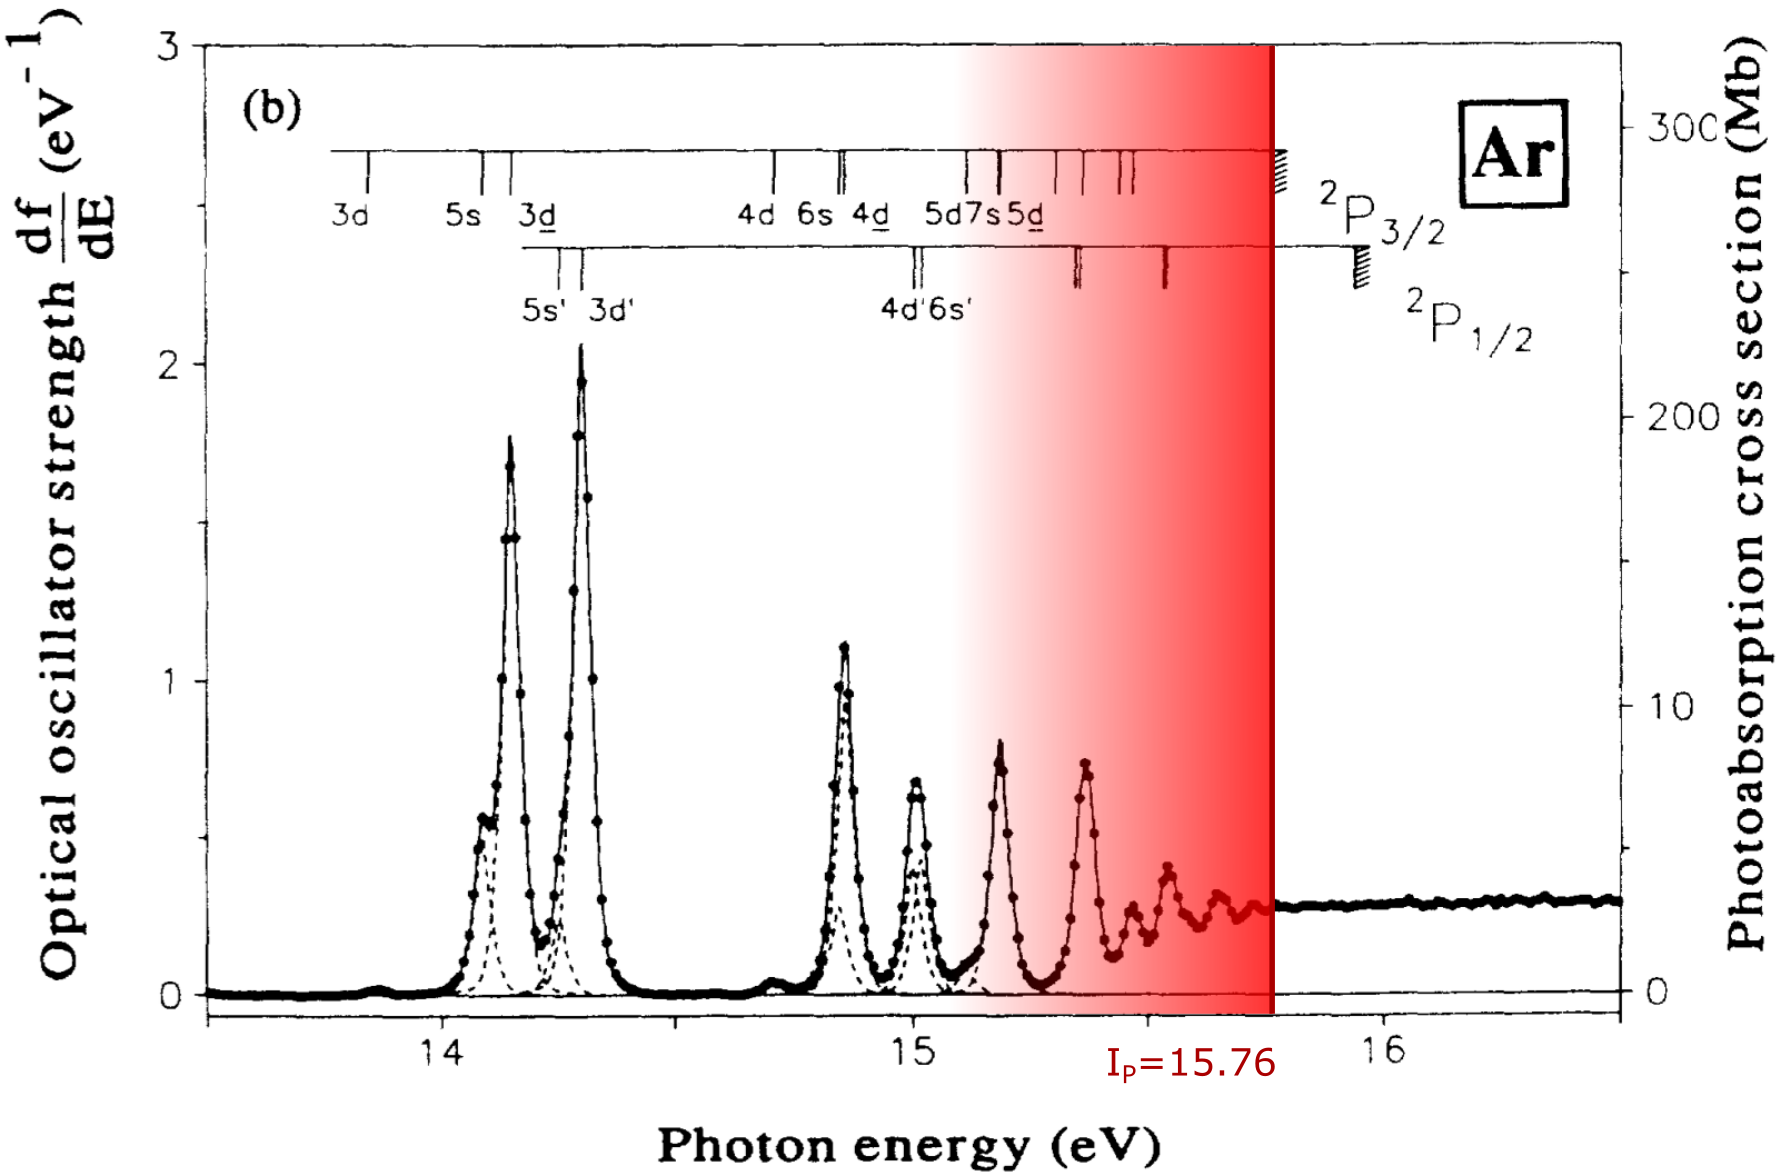
\includegraphics[width=0.9\columnwidth]{Figures/ResonantArgon/argon_spectrum.png}%
%%\caption{Section efficace de photoabsorption de l'argon dans la gamme 13.5-16.5 eV. Les lignes pointillées correspondent aux pics déconvolués. Tiré de \mycite{ChanPRA1992}.}
%%\label{fig:ArIp}%
%%\end{figure}
%%
%%Nous allons voir que cette structure bien particulière donne lieu à plusieurs phénomènes intéressants. L'argon est un système de choix car son potentiel d'ionisation ($I_p = \SI{15.76}{eV}$) est très proche de l'énergie de 10 photons d'un laser Ti:Sa ($10\times 1.55 = 15.5$ eV). L'étude de la GHOE au voisinage du potentiel d'ionisation a été réalisée expérimentalement par \mycite{ChiniNP2014}, qui observèrent une émission à la fois en dessous et au dessus du seuil. Cette émission semble avoir des caractéristiques inhabituelles par rapport à la GHOE classique. En particulier, les auteurs remarquent une augmentation du signal avec la pression sans observer de phénomène de saturation, mais n'expliquent pas le mécanisme sous-jacent. Ensuite, \mycite{XiongPRL2014} et surtout \mycite{CampPRA2015} expliquent ce mécanisme en détail et montrent qu'il est lié à la présence des états de Rydberg de la figure \ref{fig:ArIp}. Deux effets distincts interviennent dans la génération.
%%
%%Le premier est un mécanisme de GHOE résonante ayant lieu pendant l'ionisation de l'atome. Pendant la durée du pulse, tous les niveaux énergétiques de l'atome sont décalés par effet Stark. Pour les états de Rydberg de la figure \ref{fig:ArIp}, ce décalage vaut environ $U_p$, l'énergie pondéromotrice \mycite{GaardePRA2001,FiguieraPRA2002}. Ainsi, l'énergie d'un de ces niveaux peut devenir égale à l'énergie de $n$ photons infrarouges (dans notre cas, $n=10$). On a alors une résonance multi-photonique, qui augmente drastiquement l'intensité de la $n$-ième harmonique. La condition de résonance s'écrit : $n\hbar\omega = |E_R-E_0|+U_p$, où $E_R$ et $E_0$ sont respectivement les énergies de l'état fondamental et de l'état de Rydberg. Ce phénomène était déjà connu en ionisation au-dessus du seuil (ATI pour \textit{Above Threshold Ionization}) avec des impulsions courtes \mycite{FreemanPRL1987,AgostiniPRL1989}. On remarquera que pour l'argon, l'ordre harmonique résonant est le 10ème, qui n'est pas généré dans les conditions habituelles. Pour observer cet effet, on utilisera donc soit des impulsions infrarouges très courtes, soit on choisira une autre longueur d'onde de génération. Dans la suite, nous utiliserons une longueur d'onde de 400 nm, pour laquelle on a une résonance à 5 photons au seuil de l'argon.
%%
%%Le second effet ne correspond pas à la GHOE, mais produit quand même un rayonnement ultraviolet dans cette région. Dans ce mécanisme, le faisceau infrarouge crée une superposition d'état cohérente entre l'état fondamental d'énergie $E_0$ et quelques états de Rydberg d'énergie $E_R$, via une transition multiphotonique. Le dipôle ainsi créé émet une radiation d'énergie $E_R-E_0$ pendant une durée correspond à la durée de vie de l'état de Rydberg, c'est-à-dire bien plus longtemps que l'émission harmonique. Ce rayonnement a donc une structure spectrale très fine. Ce processus s'appelle \textit{Free Induction Decay} ultraviolet (xFID) \mycite{BengtssonLarsenEtAl2015}, et était déjà connu en Résonance Magnétique Nucléaire \mycite{BlockPR1946} et dans l'infrarouge \mycite{BrewerPRA1972}. 
%%
%%L'influence de ces deux effets a été étudiée expérimentalement en détail au CELIA Bordeaux par \mycite{beaulieuArXiv2016}. Des expériences réalisées à 800 nm ont permis d'observer les rayonnements issus de chacun de ces deux effets et d'étudier leurs propriétés de cohérence temporelle. Un spectre typique obtenu avec une impulsion de 7 fs est présenté sur la figure \ref{fig:xFID}. Les auteurs démontrent également la possibilité d'avoir ionisation à partir d'un état de Rydberg excité et recombinaison sur l'état fondamental, ce qui donne l'émission pointée par la ligne violette sur la figure \ref{fig:xFID}. 
%%
%%\begin{figure}[!ht]
%%\centering
%%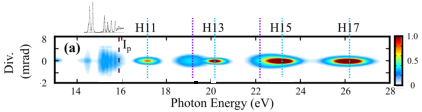
\includegraphics[width=1.1\columnwidth]{Figures/ResonantArgon/xFID.pdf}%
%%\caption{Spectre obtenu dans l'argon avec une impulsion de 7 fs à 800 nm. L'intensité est de $\SI{5.2e13}{W/cm^2}$. On observe le rayonnement xFID en dessous du seuil d'ionisation, que l'on compare avec le spectre d'absorption tiré de la figure \ref{fig:ArIp}. Ensuite, on observe les harmoniques non résonantes (lignes verticales bleues) ainsi que celles provenant d'états de Rydberg excités (lignes verticales violettes). Tiré de \mycite{beaulieuArXiv2016}.}
%%\label{fig:xFID}
%%\end{figure}
%%
%%
%
%\subsection{Ellipticité du rayonnement près du seuil de l'argon}
%\label{sec:resonant_argon_exp}
%%Pour avoir une résonance multiphonique au seuil de l'argon, nous choisissons de travailler à 400 nm. L'utilisation de cette longueur d'onde a deux autres avantages : (1) La GHOE est plus efficace, l'efficacité évolue en effet en $\lambda^{\simeq-6}$ \mycite{ShinerPRL2009}. (2) La largeur spectrale entre chaque harmonique est doublée et l'énergie de coupure diminue, on aura donc très peu d'harmoniques. Comme on le verra, ceci est très favorable dans les expériences de dichroïsme circulaire présentées plus loin. 
%%
%%Ces expériences et toutes celles qui vont suivre ont été réalisées sur le système Aurore du CELIA Bordeaux, qui délivre des impulsions de 8mJ, 25 fs à environ 800 nm et à un taux de répétition de 1 kHz. Ce faisceau est ensuite doublé en fréquence par un BBO de type 1 et de $\SI{200}{\micro\meter}$ d'épaisseur. On mesure qu'à partir de 4 mJ du fondamental, on obtient 1 mJ à 404 nm. Le 800 nm restant est filtré à l'aide de miroir dichroïques, tandis que le 400 nm est focalisé par une lentille mince de Si$\text{O}_\text{2}$ de 50 cm de focale. Le reste du dispositif est similaire à celui présenté sur la figure \ref{Fig:ExpG} : des harmoniques sont générées dans un jet de gaz continu (ouverture de $\SI{300}{\micro\meter}$) puis imagées par un réseau de diffraction couplé à une galette de micro-canaux. 
%%
%%Dans ce dispositif de GHOE assez typique, nous souhaitons rajouter une mesure de l'état de polarisation du rayonnement. Nous choisissons de mesurer des \textit{loi de Malus}. Habituellement, ces lois sont obtenues en mesurant l'intensité transmise par un polariseur parfait en fonction de l'angle du polariseur $\theta_p$ par rapport au champ électrique. Si le champ électrique est polarisé linéairement, l'intensité sera totalement transmise lorsque le polariseur est orienté parallèlement à la direction de polarisation du champ, et non transmise s'il est orthogonal. A contrario, si le champ est circulaire, l'intensité transmise ne variera pas en fonction de $\theta_p$. De manière générale, on obtient un signal oscillant de la forme 
%%\[I(\theta_p) = \epsilon^2+(1-\epsilon^2)\cos^2(\eta-\theta_p),\]
%%où $\epsilon$ et $\eta$ ont été définis dans la partie \ref{sec:polardef}. Remarquons que ce type de mesure est insensible à la partie non polarisée de la lumière, dont la contribution ne dépend pas de $\theta_p$. Ainsi, la valeur d'$\epsilon$ mesurée ici est encore une fois uniquement une borne supérieure, $\epsilon^{max}$. On voit donc que seulement pour une onde totalement polarisée, la mesure d'une loi de Malus donne accès à tous les paramètres de Stokes, définis plus haut. 
%%
%%Il reste donc à réaliser un polariseur pour le rayonnement harmonique. Nous avons déjà mentionné que les surfaces métalliques présentaient des réflexions $R_s$ et $R_p$ différentes selon chaque dimension transverse (voir section \ref{sec:metalsurface}). Ainsi, en utilisant plusieurs de ces surfaces à la suite, on peut quasiment filtrer la composante $s$ ou $p$. Nous choisissons d'utiliser trois miroirs avec revêtement en or placés à 75\degres-60\degres-75\degres, ce qui donne un rapport total $R_s/R_p$ valant 5 à 20 pour la gamme spectrale étudiée. Enfin, plutôt que de motoriser et de faire tourner ce polariseur sous vide, on préfère tourner l'orientation du champ de génération et garder le polariseur fixe, ce qui est équivalent. Ce polariseur imparfait doit être pris en compte dans l'analyse de la loi de Malus (voir \mycite{AntoinePRA1997} ainsi que \mycite{gruson}), mais n'empêche pas de mesurer les paramètres recherchés, comme l'illustre la figure \ref{fig:malus} pour l'harmonique 5. Pour plus de détail sur ce dispositif de polarimétrie harmonique on se reportera à la thèse d'Amélie Ferré \mycite{ferre}.
%%
%%\begin{figure}[!ht]
%%\centering
%%\def\svgwidth{0.7\columnwidth}
%%\import{Figures/ResonantArgon/}{malus.pdf_tex}
%%\caption{Lois de Malus pour l'harmonique 5 du faisceau à 404 nm. On mesure l'intensité transmise par le polariseur XUV en fonction de la direction de polarisation du champ de génération, lorsqu'il est polarisé linéairement (rouge) ou elliptiquement (vert). On voit que le champ harmonique est maximal en $\theta_p = \eta$, ce qui donne la direction de son ellipse de polarisation. Par ailleurs, on observe une diminution du contraste des oscillations avec $\epsilon_{IR}$, signe d'une ellipticité harmonique plus élevée. L'analyse des oscillations donne ici $\epsilon_q^{max} \simeq 0.6$ quand $\epsilon_{IR}=0.287$.}
%%\label{fig:malus}
%%\end{figure}
%%
%%La figure \ref{fig:resonant_argon_exp} présente les résultats obtenus lorsque le laser de génération porte une ellipticité $\epsilon_{IR} = 0.4$. On observe les harmoniques 5, 7 et 9 du fondamental à 404 nm. Les harmoniques 7 et 9 présentent un profil gaussien spectralement, tandis que l'harmonique 5 est structurée. Cette structure est due au xFID, effet présenté plus haut. Le rayonnement xFID est superposé à l'émission harmonique, qui est résonante due à la résonance à 5 photons.  On mesure ensuite l'ellipticité en fonction de l'énergie de photon. On voit que l'ellipticité apparente des harmoniques non résonantes est de l'ordre de $\epsilon_{IR}$, tandis que celle de l'harmonique résonante est presque doublée (valeur maximale de 0.77).  
%%
%%\begin{figure}[!ht]
%%\centering
%%\def\svgwidth{1\columnwidth}
%%\import{Figures/ResonantArgon/}{exp_result.pdf_tex}
%%\caption{Mesure d'ellipticité dans l'argon près du seuil d'ionisation. Le laser à 404 nm a une ellipticité de $\epsilon_{IR}=0.4$. Sur l'échelle de gauche (bleue), intensité en fonction de l'énergie de photon. On observe trois harmoniques, desquelles on mesure l'ellipticité apparente. On obtient les courbes rouges, échelle de droite.}
%%\label{fig:resonant_argon_exp}
%%\end{figure}
%%
%%Pour confirmer que cette forte ellipticité est due à la présence de résonances, Bernard Pons et Baptiste Fabre, du CELIA Bordeaux, ont réalisé une étude théorique du problème. On résout l'équation de Schrödinger dépendante du temps (TDSE, \textit{Time-Dependant Schrödinger Equation}) à deux dimensions, en utilisant un potentiel de Coulomb de "cœur mou", qui reproduit la présence du potentiel d'ionisation et des états sous-jacents. La figure \ref{fig:resonant_argon_th_bound} illustre ce potentiel ainsi que le spectre harmonique obtenu. On observe des structures spectrales similaires à l'expérience, à la fois dans l'intensité et dans l'ellipticité de l'harmonique 5. L'ellipticité est en particulier très modulée, mais ne prend pas des valeurs aussi élevées que celles mesurées. Au contraire, elle devient même négative à 14 eV. Les calculs ont été répétés et ont permis d'observer qu'une très légère modification du potentiel atomique donnaient lieu à de très fortes modifications de l'ellipticité. On s'attend donc à n'avoir qu'un accord qualitatif.
%%
%%\begin{figure}[!ht]
%%\centering
%%\def\svgwidth{1\columnwidth}
%%\import{Figures/ResonantArgon/}{th_result_bound.pdf_tex}
%%\caption{Résultat théorique en utilisant un potentiel de Coulomb de cœur mou. En haut, on représente le profil de ce potentiel, qui peut être ajusté pour obtenir la bonne valeur d'$\text{I}_{\text{p}}$. En bas, mêmes grandeurs que celles mesurées expérimentalement sur la figure \ref{fig:resonant_argon_exp}.}
%%\label{fig:resonant_argon_th_bound}
%%\end{figure}
%%
%%En conclusion, nous voyons que la présence de résonances sous le seuil induit une modulation de l'ellipticité. Nous mesurons de plus qu'elle augmente très fortement. On obtient donc un rayonnement aux propriétés intéressantes sans véritable perte de signal : une mesure par une photodiode calibrée montre que l'harmonique 5 contient $\num{7e6}$ photons par impulsion. De plus, le caractère résonant de l'harmonique 5 fait qu'elle ne subit pas d'effet de réabsorption \mycite{ChiniNP2014}. Son flux peut donc être facilement augmenté par une pression de génération plus élevée.  Toutefois, cette méthode est restreinte à des énergies de photons relativement basses, correspondant au seuil d'ionisation du gaz utilisé. Les gaz habituellement utilisés pour avoir un flux important sont l'argon, $\text{I}_{\text{p}}=15.76$ eV, le krypton, $\text{I}_{\text{p}}=14$ eV, ou le xénon, $\text{I}_{\text{p}}=12.13$ eV. Il serait donc intéressant de généraliser notre approche à d'autres résonances d'énergie plus élevée. Dans la section suivante, nous étudions le cas de résonances dans le continuum.
%
%\section{Génération autour d'une résonance dans le continuum}
%%Ces résonances se manifestent de la même façon que celles présentées plus haut : une augmentation de la section efficace de photoionisation. Nous nous intéressons au cas des \textit{résonances de forme} \mycite{Dehmer1972}, couramment observées dans le spectre de petites molécules. Bien qu'elles aient été observées assez tôt, leur interprétation et leur définition fait régulièrement débat, comme en témoigne l'article de \mycite{Piancastelli1999}, intitulé "\textit{The neverending story of shape resonances}" . Une interprétation courante est la suivante. Ces résonances sont dues à une barrière présente dans le potentiel moléculaire. Cette barrière est la résultante de forces attractives (e.g. coulombienne) et répulsives (effets d'écrantage, force centrifuge). Quand un photoélectron possède l'énergie correspond à cette barrière, il se retrouve dans un état métastable \mycite{simons1984roles}, piégé dans la barrière de potentiel, dont il finit par s'échapper par effet tunnel. La figure \ref{fig:shaperesonance} illustre ce principe : à l'énergie résonante, la fonction d'onde électronique est localisée sur le puit central et temporairement piégée.
%%
%%\begin{figure}[!ht]
%%\centering
%%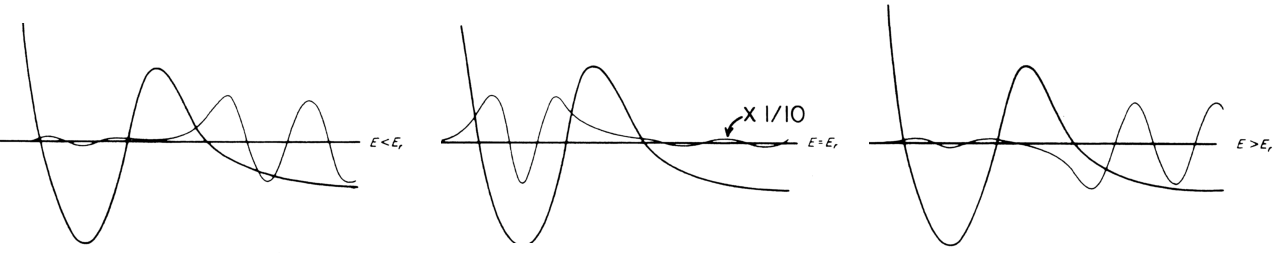
\includegraphics[width=1\columnwidth]{Figures/ResonantArgon/shape_resonance.pdf}%
%%\caption{Principe d'une résonance de forme. De gauche à droite, $E<E_r$, $E=E_r$ et $E>E_r$, où $E$ et $E_r$ sont les énergies du photoélectron et de la résonance. Tiré de \mycite{Piancastelli1999}.}
%%\label{fig:shaperesonance}
%%\end{figure}
%%
%%De par sa nature, cette barrière de potentiel se situe relativement proche de la molécule. L'électron est ainsi spatialement localisé, ce qui augmente la densité électronique et produit en général un signal de photoionisation intense. Un autre intérêt de ces résonances et que la présence d'une barrière est liée à la forme de la molécule, d'où son nom. Ainsi, de nombreux travaux ont essayé de relier l'énergie des résonances de forme aux longueurs de liaisons de molécules adsorbées, méthodes astucieusement baptisées "\textit{Bond length with a ruler}" \mycite{StohrPRL1984}.
%%
%%Nous étudions ici cet effet en ajoutant une barrière au potentiel de la figure \ref{fig:resonant_argon_th_bound} pour induire une résonance de forme vers l'énergie de l'harmonique 7. Ce potentiel ne correspond pas forcément à un système physique, mais nous permet de démontrer l'effet de la résonance du continuum. Le spectre obtenu est présenté sur la figure \ref{fig:resonant_argon_th_continuum}. On y voit le potentiel choisi, ainsi que la position de la résonance de forme. En orange, on représente une seconde résonance assez large du continuum, apparue après la modification du potentiel.
%%
%%\begin{figure}[!ht]
%%\centering
%%\def\svgwidth{1\columnwidth}
%%\import{Figures/ResonantArgon/}{th_result_continuum.pdf_tex}
%%\caption{Résultat théorique en utilisant un potentiel de Coulomb de cœur mou auquel on ajoute une barrière. Le potentiel est représenté en haut de la figure. La ligne turquoise indique la position de la résonance de forme, tandis que la zone orange est une résonance large dans le continuum également apparue après modification du potentiel. En bas, mêmes grandeurs que celles mesurées expérimentalement sur la figure \ref{fig:resonant_argon_exp}.}
%%\label{fig:resonant_argon_th_continuum}
%%\end{figure}
%%
%%Nous voyons donc que l'ellipticité de l'harmonique 7 et 9 sont significativement augmentés par la présence des deux résonances. La relation entre résonance et haute ellipticité est donc générale, ce qui permet de générer un rayonnement elliptique dans de nombreuses gammes énergétiques. Comment maintenant comprendre physiquement l'augmentation de cette ellipticité ? \mycite{StrelkovPRL2010} décrit théoriquement la GHOE près d'une résonance d'autoionisation, qui apparaît également lorsque le potentiel présente une barrière. Il montre que le modèle à trois étape habituel doit être modifié : au moment de la recombinaison, l'électron est piégé par la barrière de potentiel, le système se retrouve donc dans un état résonant du même type que celui de la figure \ref{fig:shaperesonance} avant de finalement se relaxer vers l'état fondamental en émettant un rayonnement XUV. Ce processus explique l'augmentation du signal harmonique près de la résonance par une forte section efficace de diffusion inélastique (qui contrôle le peuplement de l'état résonant) ainsi qu'une forte force d'oscillateur pour la transition entre l'état résonant et l'état fondamental.
%%Cette interprétation est tout à fait analogue à celle d'une résonance de forme en photoionisation donnée plus haut, ce qui illustre bien le caractère conjugué de ces deux effets.
%%
%%Pour vérifier que l'ellipticité est bien créée par cette étape de piégeage, Bernard Pons et Baptiste Fabre ont effectué des calculs TDSE au moment de la recombinaison. On s'intéresse au paquet d'onde électronique d'abord ionisé, qui se propage puis recombine sur l'état fondamental. Le potentiel est le même que celui présenté sur la figure \ref{fig:resonant_argon_th_continuum}. Ce paquet d'onde $\Psi(\bm{r},t)$ se décompose sur une base d'états propres de l'hamiltonien du système (voir Supplementary Information de \mycite{FerreNP2015} pour plus de détails) :
%%\[ \Psi(\bm{r},t)=\sum_{E_n>0,l} a_{E_n,l}^{(o,e)}(t)\phi_{E_n,l}^{(o,e)}(\bm{r})e^{-(\rmi E_n t)},\]
%%où $\phi_{E_n,l}^{(o,e)}$ est l'état propre d'énergie $E_n$, positive puisqu'on cherche les électrons dans le continuum, de moment angulaire $l$, et $a_{E_n,l}^{(o,e)}$ est l'amplitude. $(o,e)$ correspondent à la symétrie de l'état par rapport à l'axe $\bm{e_x}$. Si on considère la recombinaison sur un état fondamental de symétrie $s$, seulement $\phi_{E_n,1}^{e}$ et $\phi_{E_n,1}^{o}$ contribuent. Ils correspondent respectivement à l'état propre parallèle $p_x$ et perpendiculaire $p_y$. La probabilité de trouver l'électron dans un de ces états est $P_{x,y}(E_n,t) = |a_{E_n,l}^{(o,e)}(t)|^2$. On choisit $E_n$ proche de l'énergie de résonance et on considère des instants proches de l'instant de recombinaison correspondant à l'harmonique 7. Les probabilités $P_x$ et $P_y$ sont représentées sur la figure \ref{fig:resonant_proba}.
%%
%%\begin{figure}[!ht]
%%\centering
%%\def\svgwidth{1\columnwidth}
%%\import{Figures/ResonantArgon/}{electron_dynamics_resonance.pdf_tex}
%%\caption{\'{E}volution temporelle des probabilités $P_x$ (tirets bleus) et $P_y$ (traits pleins rouges) du paquet d'onde électronique arrivant sur un système présentant une résonance de forme. Le champ électrique a un cycle optique à 400 nm, une intensité pic de $\SI{10e14}{W/cm^2}$ et une ellipticité de 0.3.}
%%\label{fig:resonant_proba}
%%\end{figure}
%%
%%Nous observons que la probabilité perpendiculaire $P_y$ augmente graduellement, jusqu'à dépasser $P_x$. Ceci signifie que la résonance de forme modifie géométriquement le paquet d'onde électrique alors qu'il s'approche de l'atome. Cette augmentation de $P_y$ se manifeste dans la GHOE par une augmentation de la composante perpendiculaire du champ émis et donc de son l'ellipticité.
%
%\section{Application à la molécule de \sf6}
%\label{sec:sf6ghoe}
%%Nous appliquons maintenant expérimentalement ce résultat. L'équipe du CELIA Bordeaux a étudié en détail la génération d'harmoniques dans un gaz de molécules de \sf6 (hexafluorure de soufre). Cette molécule a une structure octaédrique avec l'atome de soufre en son centre. Le panneau du haut de la figure \ref{fig:sf6_cross_section} montre la section efficace de photoionisation de \sf6. Le canal noté C correspond à une résonance d'autoionisation \mycite{fano1968}, tandis que le canal noté A est une résonance de forme. Un calcul numérique donne la contribution de ces canaux à la GHOE (panneau du bas), qui permet de voir que la génération autour des ordres 15 à 19 est dominée par ces deux canaux. On s'attend donc à avoir un transfert efficace d'ellipticité dans cette région spectrale.
%%
%%\begin{figure}[!ht]
%%\centering
%%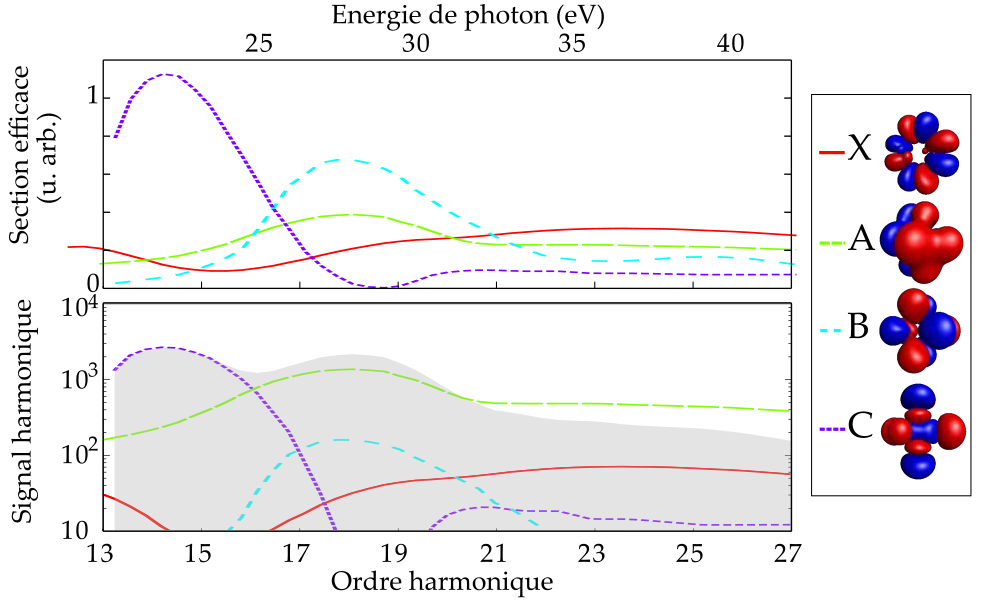
\includegraphics[width=.8\columnwidth]{Figures/SF6/sf6_cross_section.png}%
%%\caption{(Haut) Section efficace de photoionisation XUV de différents canaux d'ionisation. Extrait de \mycite{Yang98}. (Bas) Intensités des harmoniques générées par chaque canal, obtenues numériquement. La zone grisée est la superposition cohérente de tous les canaux d'ionisation. La longueur d'onde du champ de génération est 800 nm. (Droite) Orbitales moléculaires correspondant à chaque canal. Tiré de \mycite{FerreNC2015}.}
%%\label{fig:sf6_cross_section}
%%\end{figure}
%%
%%Nous avons mesuré l'ellipticité apparente du rayonnement dans cette gamme spectrale en utilisant le polariseur décrit plus haut. Les résultats sont présentés sur la figure \ref{fig:sf6_ell}. Dans un premier temps, on utilise un champ de génération à 800 nm. On observe de très hautes valeurs d'ellipticité pour les harmoniques résonantes, atteignant presque 0.8 pour l'harmonique 15 avec seulement une ellipticité de génération de 0.2. 
%%
%%\begin{figure}[!ht]
%%\centering
%%\def\svgwidth{1\columnwidth}
%%\import{Figures/SF6/}{sf6_ellipticite.pdf_tex}
%%\caption{En haut, signal harmonique produit dans \sf6 en variant l'ellipticité de génération $\epsilon_0$. En marron à jaune, impulsions de 800 nm, $\SI{1.3e14}{W/cm^2}$. En bleu foncé à clair, impulsions de 400 nm, $\SI{1.0e14}{W/cm^2}$. En bas, ellipticité apparente du rayonnement harmonique. L'erreur sur la mesure, déterminée en répétant les mesures, est de $\pm0.03$.}
%%\label{fig:sf6_ell}
%%\end{figure}
%%
%%Pour les mêmes raisons qu'expliqué auparavant, il est avantageux d'utiliser un laser de génération à 400 nm. L'expérience montre que l'on garde une ellipticité très satisfaisante : les harmoniques 5 et 7 portent respectivement une ellipticité de $\simeq 0.75$ et $\simeq 0.5$ avec $\epsilon_0=0.45$. On dispose ainsi d'une source aux propriétés remarquables, le flux étant amélioré par la génération à 400 nm. Une mesure par une photodiode calibrée montre que l'harmonique 5 contient $\num{7e6}$ photons par impulsion quand $\epsilon_0=0.3$, c'est-à-dire $\num{2e9}$ photons par seconde. Cette valeur peut être encore augmentée en utilisant par exemple des impulsions plus énergétiques et une longueur focale plus élevée.
%%
%%En conclusion, nous avons construit une source de rayonnement ultraviolet ultra-bref polarisé circulairement. Chaque harmonique considérée séparément a en effet une durée de l'ordre de la durée de l'impulsion de génération, c'est-à-dire $\simeq 20$ femtosecondes, ce qui en fait une alternative particulièrement intéressante aux sources synchrotrons malgré son flux moindre. Comparé aux lasers à électron libre, eux aussi capables de produire des polarisation circulaires \mycite{AllariaPRX2014}, le flux est bien sûr bien moindre, mais le taux de répétition et la résolution temporelle fournis par la GHOE sont très avantageux pour des mesures de spectroscopie moléculaire. Dans la suite nous démontrerons ce point en effectuant des expériences de photoionisation sur des molécules chirales. 
%%%
%\chapter{Polarisation circulaire et chiralité}
%\section{Définitions de la chiralité}
%\subsection{Molécules chirales}
%%Le concept de polarisation de la lumière est historiquement lié à celui de la \textit{chiralité}. En 1808, Malus observa que la lumière réfléchie par une substance diaphane possédait une polarisation (mot qu'il introduisit en 1810). Cette polarisation était mise en évidence par une transmission à travers un cristal de calcite. Cette propriété fut observée par Arago dans des cristaux de quartz, avant d'être étudiée par Biot qui en 1812 montra que différents types de quartz tournaient la direction de polarisation soit à droite soit à gauche, propriété appelée \textit{activité optique}. Il mesura le même effet dans des substances organiques telles que des molécules de camphre. En 1848, Pasteur relia cette propriété optique à la géométrie du cristal ou de la molécule considérée. Il émit l'idée que certaines molécules existaient sous des formes géométriques dissymétriques tout en ayant les mêmes propriétés chimiques. Le mot de \textit{chiralité} fut introduit en 1893 par Lord Kelvin durant la deuxième "Robert Boyle Lecture" à l'université d'Oxford \mycite{kelvin1894} :
%%\begin{quotation}
%%I call any geometrical figure, or group of points, 'chiral', and say that it has chirality if its image in a plane mirror, ideally realized, cannot be brought to coincide with itself.
%%\end{quotation}
%%Le terme de chiralité dérive du mot grec sigifiant "main", un exemple d'objet chiral (voir figure \ref{fig:chirality}). Les deux formes possèdent un pouvoir rotatoire opposé et sont nommées \textit{énantiomères} (formes opposées en grec). On peut les nommer selon le signe de la rotation qu'ils imposent à la lumière : on parle alors de molécule dextrogyre (D ou +) ou lévogire (L ou -). Cependant, une même molécule peut imposer une rotation gauche ou droite selon la longueur d'onde de la lumière utilisée. On utilise donc également la configuration absolue de la molécule, définie à partir de sa structure tri-dimensionelle. On note alors les énantiomère R (rectus) et S (sinister). La configuration absolue d'une molécule est habituellement mesurée par diffraction X \mycite{Bijvoet1951}, par explosion coulombienne \mycite{pitzer2013} ou encore par spectroscopie micro-onde \mycite{patterson2013}.
%%
%%\begin{figure}[!ht]
%%\centering
%%\includegraphics[width=.5\columnwidth]{Figures/Chirality/chirality_with_hands.pdf}%
%%\caption{Une molécule "chirale" n'est pas superposable à son image dans un miroir. De même que les mains gauches et droites ont un pouce et des doigts dans le même ordre, les molécules chirales ont les mêmes atomes dans le même ordre mais ne sont pas images l'une de l'autre dans un miroir.}
%%\label{fig:chirality}
%%\end{figure}
%
%\subsection{La chiralité de la lumière}
%%Deux énantiomères ont les mêmes propriétés chimiques. Cependant, elles interagiront différemment avec un objet lui-même chiral. Par exemple, la plupart des récepteurs biologiques sont chiraux et réagiront très différemment à une protéine R ou S. Le contrôle et la mesure des propriétés chirales sont donc centraux dans l'industrie alimentaire, pharmaceutique et cosmétique. 
%%
%%Les expériences mentionnées montrent que la lumière permet de caractériser une molécule chirale, ce qui implique que la lumière elle-même doit être un objet chiral. La définition donnée plus haut est insuffisante, car comme noté par Lord Kelvin dans ses \textit{Baltimore Lecture}, elle ne permet pas de distinguer les effets due à la chiralité de ceux dues à d'autres types de dissymétries telles que l'effet Faraday. \mycite{Barron1986} donne une définition généralisable à la chiralité de particules élémentaires telles qu'un photon :
%%
%%\begin{quotation}
%%True chirality is exhibited by systems that exist in two distinct enantiomeric (enantiomorphic) states that are interconverted by space inversion, but not by time reversal combined with any proper spatial rotation.
%%\end{quotation}
%%
%%Cette définition permet de distinguer la "vraie" chiralité de la fausse, c'est-à-dire une chiralité indépendante du temps. Les opérations spatiales et temporelles décrites sont représentées sur la figure \ref{fig:truefalsechir}, où elles sont notées T (inversion du temps), P (inversion de l'espace), et $\text{R}_{\pi}$ (rotation, ici d'angle $\pi$). 
%%
%%\begin{figure}[!ht]
%%\centering
%%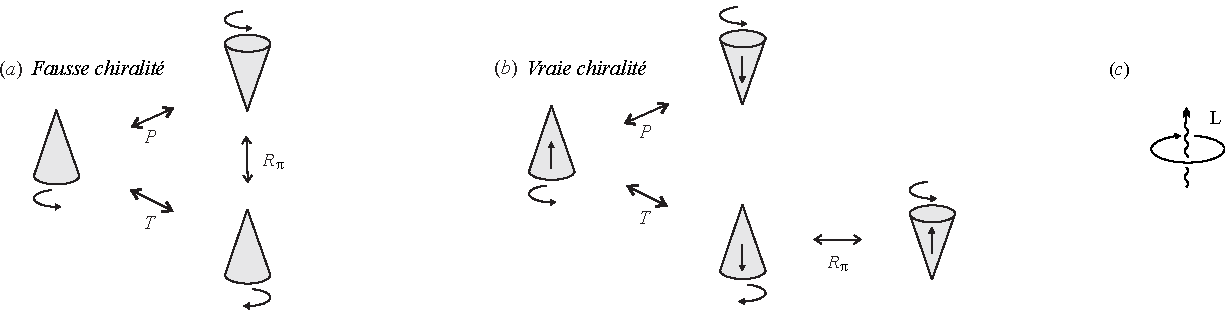
\includegraphics[width=.9\columnwidth]{Figures/Chirality/truefalsechir.pdf}%
%%\caption{Vraie et fausse chiralité. \textit{(a)} Cône en rotation immobile. P (inversion de l'espace) donne le même résultat que T (inversion du temps) suivi de $\text{R}_{\pi}$ (rotation d'angle $\pi$). \textit{(b)} Cône en rotation en translation. Il présente cette fois une vraie chiralité. \textit{(c)} Lumière polarisée circulairement : un photon est analogue au cône en translation. Tiré de \mycite{barron}.}
%%\label{fig:truefalsechir}
%%\end{figure}
%%
%%Dans cette figure, on prend l'exemple d'un cône en rotation. Si le cône est immobile, P donne la même chose que T suivi de $\text{R}_{\pi}$, il ne présente pas de vraie chiralité. Au contraire, s'il est en translation, il a une vraie chiralité. Le cas du photon est similaire, l'hélicité du photon pouvant être vue classiquement comme une rotation. Le photon ne peut de plus pas être immobile, la lumière polarisée circulairement est donc chirale selon cette définition. Pour des molécules chirales, on appelle mélange \textit{racémique} un mélange composé d'autant de chacun des deux énantiomères. Ceci est analogue à une lumière polarisée linéairement, constituée d'autant de photons polarisés circulairement droit que gauche. 
%%
%%La lumière polarisée circulairement est donc un outil de choix pour sonder et caractériser les molécules chirales. De nombreuses interactions sont possibles, nous décrirons dans la section suivante celle nommée dichroïsme circulaire, avant de présenter le dichroïsme circulaire de photoélectron, que nous mesurerons avec la source décrite dans la partie \ref{CH:Circular_HHG}.
%
%\section{Dichroïsme circulaire d'absorption}
%%Fresnel expliqua le phénomène d'activité optique par une différence de vitesse de propagation de la composante circulaire droite (notée D) et gauche (G) d'une onde polarisée linéairement. Le milieu présente donc un indice de réfraction pour chaque composante. Considèrons un champ polarisé linéairement tel que les vecteurs champs électriques RCP et LCP soient parallèles à $z = 0$. Après une propagation sur une distance $L$, les champs auront tourné de $\theta^{G}=2\pi\rmc L/(\lambda v^{G})$ et $\theta^{R}=-2\pi\rmc L/(\lambda v^{RCP})$. L'angle de rotation de la direction du champ s'écrit alors :
%%\begin{align*}
%%\chi = \frac{1}{2}(\theta^{G}+\theta^{D}) &= \frac{\pi\rmc L}{\lambda}\left(\frac{1}{v^{G}}-\frac{1}{v^{D}}\right)\\
%%&= \frac{\pi}{\lambda}\left(n^{G}-n^{D}\right).
%%\end{align*}
%%
%%Mais si $n^{G}$ et $n^{D}$ sont différents, le milieu doit également absorber différemment chaque composante du champ. Cet effet a été mesuré pour la première fois par \mycite{Haidinger1847} puis étudié par \mycite{Cotton1895}, qui le nomma \textit{dichroïsme circulaire}. Cet effet est toujours couramment utilisé avec des longueurs d'ondes visibles ou infrarouges. Il est généralement préféré à la mesure de l'activité optique car il évolue plus rapidement avec la longueur d'onde, et permet donc de distinguer plus facilement différentes bandes spectrales. Le dichroïsme circulaire est ainsi utilisé pour la détermination de structures de protéines, de changements de structures induits par par exemple le pH ou le solvant, de repliements/dépliements de protéines, ou encore de liaison de ligands.
%%
%%L'absorption correspond à une transition d'un état initial vers un état excité. Lorsque la lumière traverse un ensemble de molécule, son intensité est gouvernée par la loi de Beer-Lambert, c'est-à-dire une décroissance exponentielle en fonction de la longueur parcourue. On note $\alpha^{D}$ et $\alpha^{G}$ les coefficients d'absorption de chacune des composantes du champ. Le dichroïsme circulaire vaut :
%%\[\Delta \alpha = \alpha^{G}-\alpha^{D}.\]
%%En pratique, on préfère utiliser le ratio entre le dichroïsme circulaire et l'absorption habituelle, appelé facteur de dissymétrie \mycite{Kuhn1930} : 
%%\begin{equation}
%%g = \frac{\alpha^{G}-\alpha^{D}}{\frac{1}{2}(\alpha^{G}+\alpha^{D})}.
%%\label{eq:kuhn}
%%\end{equation}
%%
%%Relions $\alpha$ aux propriétés de la molécule. Pour une longueur de propagation $\delta z$ dans le milieu infinitésimale, l'intensité absorbée par unité de surface $\delta I$ s'écrit :
%%\begin{align*}
%%\frac{\delta I}{I} = \alpha c \delta z,
%%\end{align*}
%%où $c$ est le nombre de molécule par mètre cube. On note $w$ l'énergie moyenne absorbée par molécule, on a donc $\delta I = c \delta z w$. On obtient alors :
%%\begin{align}
%%\alpha = \frac{\delta I}{Ic \delta z} = \frac{c \delta z w}{Ic \delta z} = \frac{w}{I}.
%%\label{eq:cd1}
%%\end{align}
%%Notons qu'un facteur de proportionnalité s'ajoute à cette expression si on choisit d'utiliser un coefficient d'absorption molaire.
%%
%%Considérons maintenant la transition électronique $i\rightarrow f$. \`A cette transition est associé un élément de matrice de transition qu'on note $V_{if}$. La bande d'absorption a un profil spectral qui donne la probabilité de transition en fonction de la fréquence, qu'on note $\rho(\omega)$. \mycite{schellman1975} montre que ces quantités sont reliés à $w$ par la relation :
%%\begin{equation}
%%w(\omega) = \frac{\pi \omega |V_{if}|^2 \rho(\omega)}{2\hbar}.
%%\label{eq:cd2}
%%\end{equation}
%%
%%Il faut donc déterminer $V_{if}$ pour obtenir $\alpha$. Commençons dans l'approximation dipolaire électrique. Dans ce cas, le champ électrique se couple avec le moment dipolaire de la molécule : $V_{if} = -\bm{\mu}_{if}\cdot \bm{E}$, où $\mu_{if}$ est le moment dipolaire (voir partie \ref{sec:multipolar}). \mycite{schellman1975} montre que si le champ est polarisé circulairement droite ou gauche, on a $(V_{if}^{D/G})^2 = (\bm{\mu}_{if})^2E^2_0/3$, où la division par 3 provient d'une moyenne sur les orientation possibles des moments dipolaires.
%%On utilise alors les équations \ref{eq:cd1} et \ref{eq:cd2} :
%%\begin{align*}
%%\alpha^{D/G}(\omega) &= \frac{w^{D/G}(\omega)}{I} = \frac{\pi \omega |V_{if}^{D/G}|^2 \rho(\omega)}{2\hbar I} 
%%= \frac{\pi \omega |\mu_{if}E_0|^2 \rho(\omega)}{6\hbar I} 
%%= \frac{\pi \omega |\mu_{if}|^2 \rho(\omega)E^2_0}{6\hbar I} \\
%%&= \frac{4\pi^2 \omega |\mu_{if}|^2 \rho(\omega)}{3\hbar n \rmc} 
%%\end{align*}
%%On obtient donc directement le dichroïsme circulaire : $\Delta\alpha = \alpha^G-\alpha^D = 0$. Dans l'approximation dipolaire, le dichroïsme circulaire est donc nul. \par Il faut considérer le terme suivant du développement multipolaire : 
%%\[V_{if} = -\bm{\mu}_{if}\cdot \bm{E} - \bm{m}_{if}\cdot \bm{B}.\] 
%%\mycite{schellman1975} réalise le calcul de $V_{if}$ pour une polarisation circulaire :
%%\begin{align*}
%%(V_{if}^{D/G})^2 &= \frac{(\bm{\mu}_{if})^2E^2_0}{3}+\frac{(\bm{m}_{if})^2B^2_0}{3} \mp \frac{2}{3}\text{Im}(\bm{\mu}_{if}\cdot\bm{m}_{if})E_0B_0 \\
%%&= \frac{8\pi I}{3 \rmc}\left[\frac{(\bm{\mu}_{if})^2}{n} +  n(\bm{m}_{if})^2 \mp 2 \text{Im}(\bm{\mu}_{if}\cdot\bm{m}_{if})\right]. 
%%\end{align*}
%%Chacun des trois terme a sa propre probabilité de transition, qu'on note $\rho(\omega)$, $\tau(\omega)$ et $\sigma(\omega)$. On obtient donc pour le coefficient d'atténuation :
%%\begin{equation*}
%%\alpha^{D/G}(\omega) = \frac{4\pi^2 \omega}{3\hbar \rmc}\left[\frac{\rho(\omega)(\bm{\mu}_{if})^2}{n} +  n\tau(\omega)(\bm{m}_{if})^2 \mp 2 \sigma(\omega)\text{Im}(\bm{\mu}_{if}\cdot\bm{m}_{if})\right] 
%%\end{equation*}
%%
%%Les trois termes obtenus correspondent à l'absorption dipolaire électrique, l'absorption dipolaire magnétique, et le dichroïsme circulaire. En effet, on obtient :
%%\[ \Delta \alpha = \alpha^G-\alpha^D = \frac{16\pi^2 \omega\sigma(\omega)\text{Im}(\bm{\mu}_{if}\cdot\bm{m}_{if})}{3\hbar \rmc}. \]
%%Le fait que l'on ait besoin d'utiliser l'approximation dipolaire magnétique pour observer du dichroïsme circulaire signifie que cet effet sera faible en général. Ainsi, le facteur d'asymétrie $g$ (équation \ref{eq:kuhn}) a des valeurs typiques de $10^{-5}\text{-}10^{-3}$ \mycite{Levi1980}. Ceci impose de réaliser des mesures à densité élevée, c'est-à-dire en phase liquide ou sur des films minces. La mesure est alors parasitée par la contribution du solvant ou du substrat, empêchant la mesure du dichroïsme de la molécule libre.
%%\clearpage
%\section{Dichroïsme circulaire de photoélectron (PECD)}
%\label{sec:PECD}
%%On s'intéresse désormais à un autre type de dichroïsme, qui comme nous allons voir a des propriétés très différentes. Jusque ici, nous avons présenté des techniques chiroptiques (terme désignant l'étude de molécule chirales par la lumière) dans le domaine visible ou proche infrarouge. Le passage à des énergies de photon plus élevées donne accès à un phénomène supplémentaire : la photoionisation. Nous allons donc décrire l'émission d'un électron par une molécule chirale suite à l'absorption de lumière polarisée circulairement. 
%%
%%On considère une impulsion lumineuse se propageant selon la direction $e_z$. On place une molécule chirale au centre d'un repère sphérique $(r,\theta,\phi)$, où $r$ est la position du photoélectron, $\theta$ est l'angle par rapport à l'axe $e_z$, comme représenté sur la figure \ref{fig:geomPECD}.
%%
%%\begin{figure}[!ht]
%%\centering
%%\def\svgwidth{0.5\columnwidth}
%%\import{Figures/PECD/}{geomPECD.pdf_tex}
%%\caption{Géométrie de photoionisation.}
%%\label{fig:geomPECD}
%%\end{figure}
%%
%%Dans le cas de molécules chirales d'orientation aléatoire et d'un champ parfaitement polarisé, le phénomène ne dépend pas de $\phi$. En 1976, \mycite{RitchiePRA1976} obtint l'expression de la distribution angulaire des photoélectrons éjectés et montra qu'elle prend la forme suivante :
%%\begin{equation}
%%I^p(r,\theta) = b_0^p(r) + b_1^p(r) P_1(\cos\theta) + b_2^p(r) P_2(\cos\theta)
%%\label{eq:angulardistrib}
%%\end{equation}
%%où les $b_i$ sont des fonctions du potentiel moléculaire, de l'énergie $h\nu$ et de la polarisation $p$ du photon incident ($p = 0$, polarisation linéaire, $p =\pm1$ polarisation circulaire gauche/droite). Les $P_i$ sont les polynômes de Legendre, qui valent $P_1(x) = x$ et $P_2(x) = (3x^2-1)/2$. Il est important de noter que contrairement à celui du dichroïsme circulaire, ce calcul a été réalisé dans l'approximation dipolaire électrique. Le calcul complet des $b_i$ permet d'obtenir les propriétés suivantes :
%%\begin{align}
%%b_0^1 &= b_0^{-1} \nonumber\\
%%b_1^0 &= 0\nonumber\\
%%b_1^1 &= -b_1^{-1}\nonumber\\
%%b_2^1 &= b_2^{-1}.
%%\label{eq:bi}
%%\end{align}
%%$b_0$ est couramment appelé PES (Photo Emission Spectrum), et correspond simplement à la section efficace de photoionisation de la molécule. $b_2$ est souvent noté $\beta$ et appelé paramètre d'anisotropie. Quant à $b_1$, on remarque qu'il fait apparaître un dichroïsme :
%%\begin{equation}
%%I^{1}(r,\theta)-I^{-1}(r,\theta) = (b_1^1(r)-b_1^{-1}(r))P_1(\cos\theta) = 2b_1^1(r)\cos\theta
%%\label{eq:pecddef}
%%\end{equation}
%%On obtient donc une asymétrie autour de $\theta = 90\degres$, c'est-à-dire avant-arrière par rapport à la direction de propagation de la lumière. Cet effet est appelé dichroïsme circulaire de photoélectron (PECD, \textit{PhotoElectron Circular Dichroism}), et $b_1$ est le \textit{paramètre dichroïque}. On note souvent $PECD = 2b_1$. L'équation \ref{eq:bi} montre directement que le PECD change de signe si on change l'hélicité de la lumière. De même, le signe change si on change d'énantiomère.
%%
%%\mycite{PowisJPCA2000} obtint théoriquement des asymétries allant jusqu'à 40\% de la section efficace totale. Des démonstrations expérimentales n'ont pas tardé à arriver, profitant du développement de sources synchrotrons fournissant de la lumière XUV polarisée circulairement. \mycite{BoweringPRL2001} ont mesuré le PECD du bromocamphre en 2001, avant que \mycite{GarciaJCP2003} étudient le camphre et \mycite{TurchiniJACS2004} le methyloxirane. L'asymétrie la plus haute aujourd'hui mesurée est de 32\% \mycite{DalyJCP2011}. Ces valeurs élevées s'expliquent par le caractère purement dipolaire électrique du PECD et permettent de réaliser des études chiroptiques en phase gazeuse.
%%Par la suite, l'étude du PECD a montré son impressionnante sensibilité aux finesses du potentiel moléculaire. Tout d'abord, $b_1$ est différent selon l'orbitale ionisée, comme démontré dans le camphre par \mycite{NahonJCP2006}. Ensuite, le PECD peut varier drastiquement avec des substitutions chimiques, comme illustré sur la figure \ref{fig:substitution}, tirée de \mycite{Tia2014}. On y voit qu'en changeant un élément de la molécule, la section efficace et le paramètre $\beta$ ne changent presque pas, car l'orbitale ionisée est localisé sur l'atome d'oxygène. Cependant, le paramètre $b_1$ évolue drastiquement, permettant de différencier les quatres molécules. Un autre exemple est celui des conformères, qui sont des molécules de même formule mais dont les atomes ont tourné autour d'une liaison chimique. Le PECD est également capable de distinguer ces deux molécules \mycite{GarciaPCCP2008}. Pour finir, il a récemment été observé que le PECD était sensible aux modes de vibration, c'est-à-dire aux mouvements des noyaux \mycite{GarciaNC2013}.
%%
%%\begin{figure}[!ht]
%%\centering
%%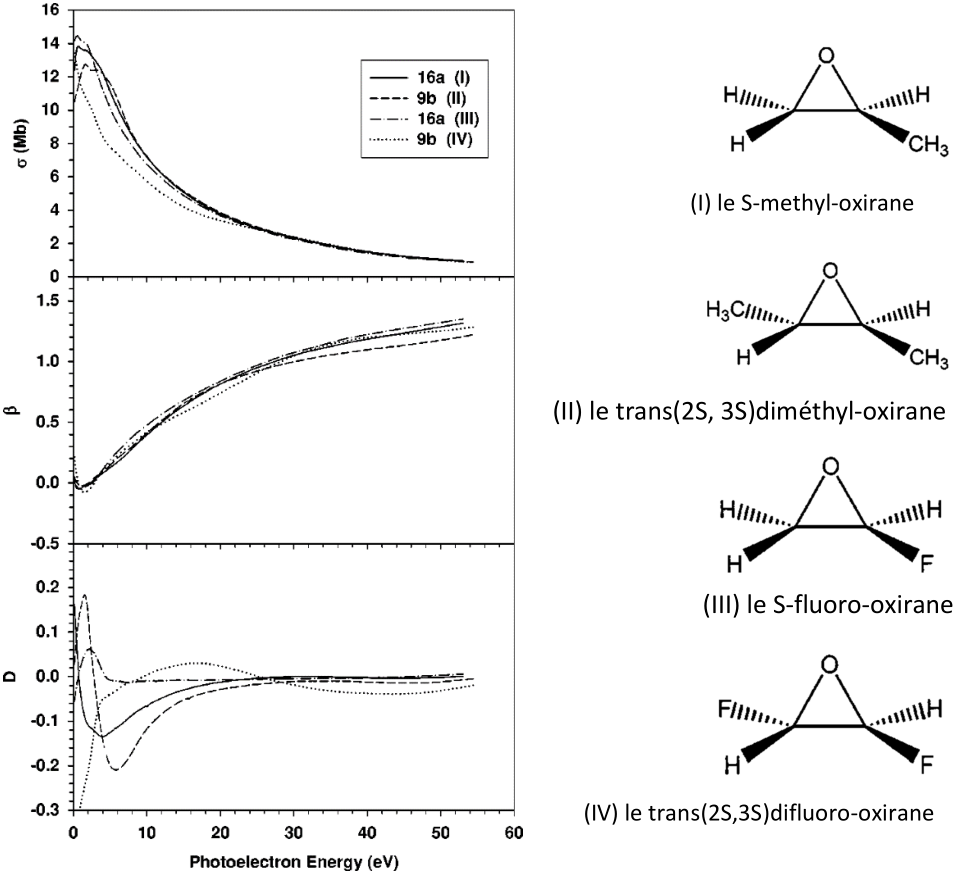
\includegraphics[width=.7\columnwidth]{Figures/PECD/substitution.png}%
%%\caption{Effet d'une substitution sur le PECD. Quatres molécules sont représentées à droite. \`A gauche, on voit leur section efficace de photoionisation $\sigma$, leur paramètre d'anisotropie $\beta$ et le paramètre dichroïque $b_1$, ici noté D. Tiré de \mycite{Tia2014}.}
%%\label{fig:substitution}
%%\end{figure}
%%
%%Cette haute sensibilité au détails fins du potentiel moléculaire peut être expliquée dans un modèle où un électron diffuse sur la molécule après avoir été ionisé. On part d'un état initial où l'électron est lié, et on observe l'électron dans le continuum après qu'il ait diffusé sur le potentiel moléculaire. \mycite{DillDehmer1974} montrent que la fonction d'onde du photoélectron dans le continuum se décompose en différentes composantes de moment angulaire défini. Chacune de ces composante est déphasée différemment par le potentiel moléculaire. La phase de chaque composante $\ell$, que l'on note $\sigma_\ell$, est responsable d'interférences dans le continuum entre ondes partielles. Ainsi, une observable sera d'autant plus sensible au potentiel moléculaire qu'elle est sensible à des petites variations de $\sigma_\ell$. Le calcul de \mycite{RitchiePRA1976} donne les dépendances en $\sigma_\ell$ des $b_i$ :
%%
%%\begin{itemize}
%%\renewcommand{\labelitemi}{$\bullet$}
%%\setlength\itemsep{1em}
%%\item $b_0$ ne dépend pas du tout de $\sigma_\ell$. La section efficace intégrée sur tout l'espace ne présente donc que peu d'information.
%%\item $b_2$ dépend de $\sigma_\ell$ pour une valeur de $\ell$ sur deux. Plus précisément, $b_2$ présente un terme $\cos(\sigma_\ell-\sigma_{\ell+2})$. $b_2$ fournit donc davantage d'information que la section efficace totale.
%%\item Le cas qui nous intéresse est celui de $b_1$, qui lui présente un terme $\sin(\sigma_\ell-\sigma_{\ell+1})$. Toutes les composantes $\ell$ influent donc sur sa valeur. De plus, on a une dépendance en sinus, qui varie significativement pour des petites valeurs de déphasage entre composantes $\ell$. Au contraire, le cosinus dans l'expression de $b_2$ est relativement plat au voisinnage de $\sigma_\ell-\sigma_{\ell+2} = 0$.
%%\end{itemize}
%%
%%Nous avons jusque ici mentionné des études réalisées sur synchrotron. Ces travaux présentent une très bonne résolution spectrale, mais faute de source adaptée, aucune étude \textit{dynamique} du PECD n'a été réalisée. Nous allons utiliser la source présentée en partie \ref{CH:Circular_HHG} à cet effet.
%%%
%\chapter{Mesures de PECD avec une source d'harmoniques d'ordre élevé}
%\section{Dispositif expérimental}
%\subsubsection{Source de lumière}
%%Nous utilisons la source décrite en partie \ref{CH:Circular_HHG}, dont nous rappelons brièvement les propriétés : le système laser Aurore délivre des impulsions à $\simeq$800 nm, qui sont doublées dans un cristal de BBO de type 1 de 200 $\si{\micro\metre}$. On dispose alors d'impulsions de 1 mJ à 404 nm à une fréquence de 1 kHz. Pour mesurer un PECD, il est pratique d'alterner successivement polarisations circulaires droite et gauche et de faire la différence entre elles, de sorte à éviter des effets de dérive lente. Pour ce faire, il faut alterner la polarisation du champ de génération à 404 nm. On utilise une lame demi-onde d'ordre 0 large bande placée avant une lame quart d'onde. L'orientation de la lame quart d'onde est fixe selon l'axe vertical. On peut ainsi tourner la lame demi-onde d'un angle $\pm\beta/2$ pour obtenir une ellipticité $\epsilon_0 = \pm \tan\beta$, tout en gardant l'axe de l'ellipse vertical après les lames d'onde. On choisit ici $\epsilon_0 = \pm 0.3$. La figure \ref{fig:waveplates} illustre le fonctionnement du dispositif. Le rayonnement est ensuite focalisé dans un jet de \sf6 par lentille de $\text{SiO}_2$ de 50 cm de focale. Les harmoniques générées sont alors polarisées elliptiquement et d'ellipticité de même signe que celui du fondamental. Les valeurs d'ellipticité apparentes ont été présentées plus haut (voir figure \ref{fig:sf6_ell}).
%%
%%\begin{figure}[!ht]
%%\centering
%%\def\svgwidth{0.7\columnwidth}
%%\import{Figures/PECD/}{waveplates.pdf_tex}
%%\caption{Contrôle de l'état de polarisation du fondamental. De gauche à droite : état de polarisation avant les lames d'onde, état après une lame demi-onde d'angle $\pm\beta/2$, état après une lame quart d'onde orientée verticalement.}
%%\label{fig:waveplates}
%%\end{figure}
%
%\subsubsection{Détection : spectromètre imageur de vecteur vitesse}
%%Le champ harmonique produit par les molécules de \sf6 est alors utilisé pour photoioniser un gaz de molécules chirales. Pour ne pas modifier l'état de polarisation du champ, on n'introduit aucune optique entre la source et la zone de détection. Seul un iris permet d'ajuster l'intensité envoyée dans le gaz de molécule. La mesure du PECD de ces molécules nécessite de connaître l'énergie et la direction d'émission des photoélectron créés lors de la photoionisation. Expérimentalement, ceci est réalisé à l'aide d'un spectromètre imageur de vecteur vitesse (VMI pour \textit{Velocity Map Imager}). 
%%
%%Le fonctionnement de cet appareil est représenté sur la figure \ref{fig:vmi}. Le faisceau harmonique croise un jet moléculaire, dont le recouvrement définit la zone d'interaction. La photoionisation a lieu dans cette zone, et crée un nuage d'espèces chargées (ions et électrons). Autour de cette zone sont positionnées trois électrodes servant à collecter ces espèces chargées. Ces électrodes forment une \textit{lentille électrostatique} qui vient focaliser les espèces chargées sur un détecteur placé perpendiculairement à l'axe de propagation de la lumière, constitué de galettes de micro-canaux (MCP) et d'un écran de phosphore. L'électrode la plus éloignée du détecteur repousse les espèces et est donc appelée répulseur. L'électrode intermédiaire est appelée extracteur, tandis que la troisième est l'électrode de masse car son potentiel est nul. Le signe des potentiels permet de collecter les ions ou bien les électrons émis lors de l'interaction. 
%%
%%\begin{figure}[!ht]
%%\centering
%%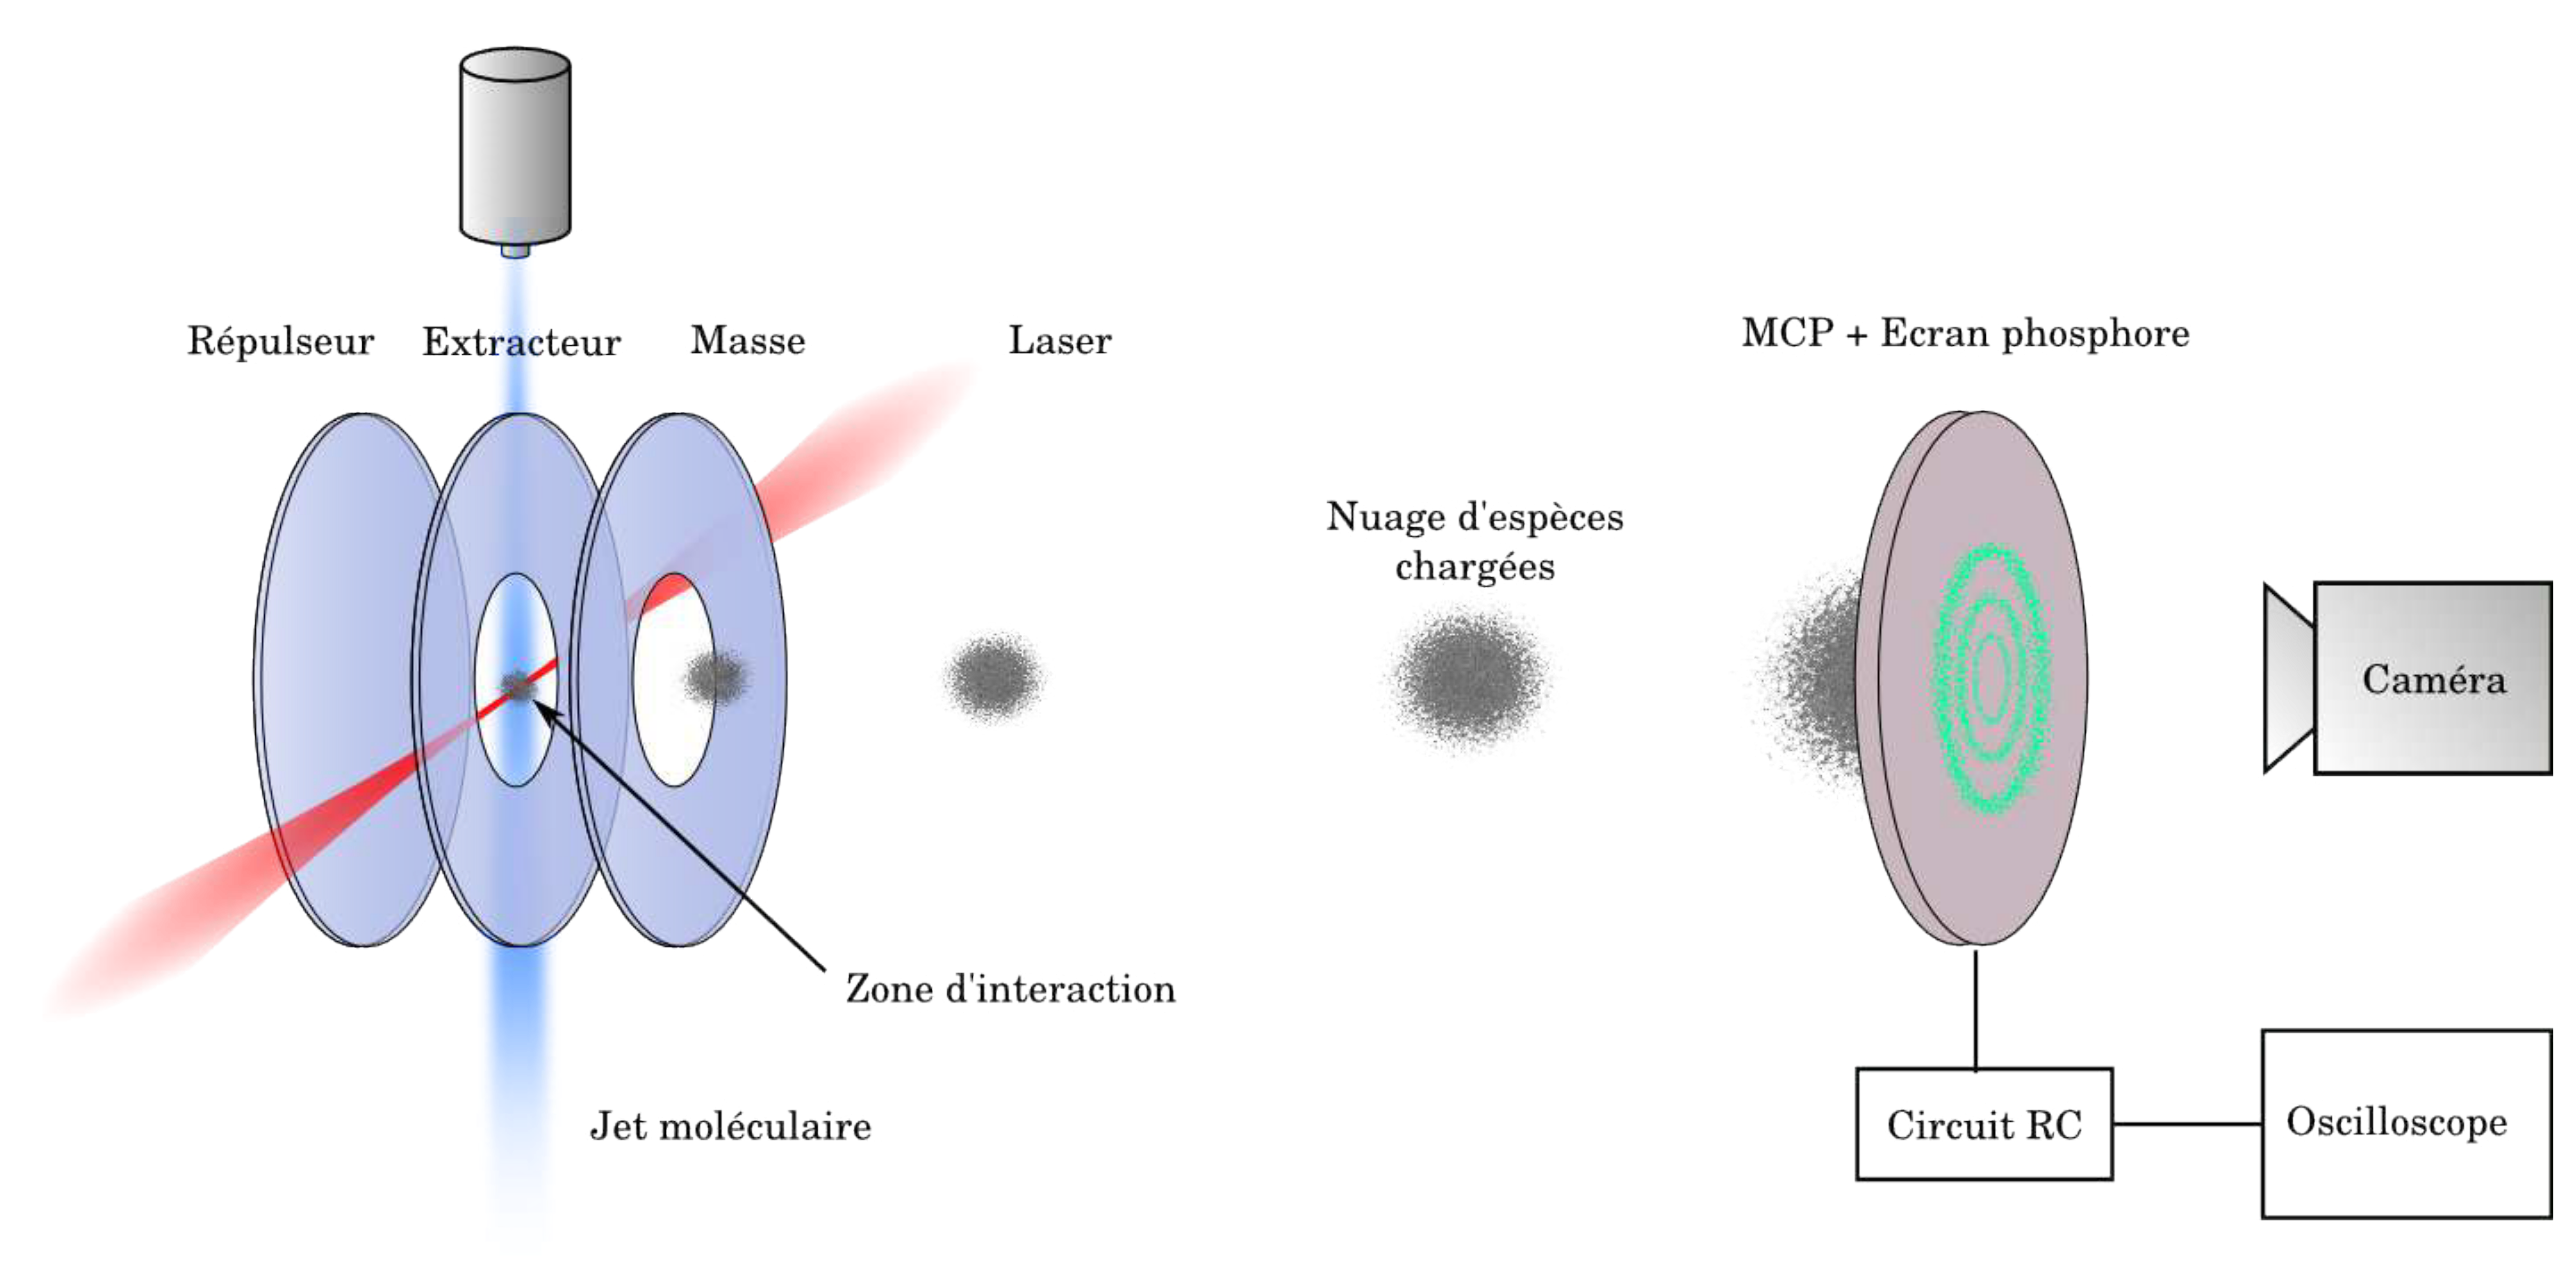
\includegraphics[width=1\columnwidth]{Figures/PECD/vmi.png}%
%%\caption{Schéma représentatif du fonctionnement d'un VMI (Spectromètre imageur de vecteur vitesse). Tiré de \mycite{handschin}.}
%%\label{fig:vmi}
%%\end{figure}
%%
%%Les deux dernières électrodes de l'appareil sont percées en leur centre, amélioration majeure proposée par \mycite{EppinkParker1997}. L'instrument ainsi réalisé possède des propriétés remarquables. D'abord, les particules sont collectées dans un angle solide avoisinant les $4\pi$ stéradians. De plus, quand la lentille électrostatique est optimisée, toutes les particules de même vecteur vitesse sont focalisées en un unique point du détecteur, quelque soit le lieu où elles ont été émises. C'est cette propriété qui donne son nom à ce spectromètre de vecteur vitesse. On trouvera une discussion très détaillée sur la conception de cet appareil dans la thèse de C. Handschin \mycite{handschin}.
%
%\section{Résultats dans la fenchone}
%\label{sec:results_fenchone}
%%Nous choisissons un système déjà étudié sur synchrotron : la molécule de fenchone ($\text{C}_{10}\text{H}_{16}\text{O}$). Elle possède deux énantiomères, représentés sur la figure \ref{fig:fenchone}. On notera Fenchone (+) l'énantiomère de nom systématique  (1S,4R)-1,3,3-triméthylbicyclo[2.2.1]heptan-2-one et Fenchone (-) l'énantiomère (1R,4S)-1,3,3-triméthylbicyclo[2.2.1]heptan-2-one. L'orbitale moléculaire la plus haute occupée (HOMO) est d'énergie $\simeq$8.6 eV. Les suivantes sont HOMO-1 (10.4 eV), HOMO-2 (10.7 eV), HOMO-3 (11.2 eV), etc. Les valeurs de potentiel d'ionisation ont été obtenus expérimentalement sur synchrotron \mycite{PowisCPC2008}. On voit donc que la troisième harmonique, d'énergie 9 eV, est suffisante pour ioniser la HOMO.
%%
%%\begin{figure}[!ht]
%%\centering
%%\def\svgwidth{0.7\columnwidth}
%%\import{Figures/PECD/}{fenchone.pdf_tex}
%%\caption{\'{E}nantiomères de la molécule de fenchone.}
%%\label{fig:fenchone}
%%\end{figure}
%%
%%Pour la mesure de PECD, nous avons utilisé un VMI initialement développé par Valérie Blanchet et Charles Handschin. Un réservoir rempli d'un des deux énantiomères (fourni par Sigma-Aldrich, pureté énantiomérique $\simeq$99\%) est connecté à une buse métallique chauffée à 120\degres C de 300 $\si{\micro\metre}$ de diamètre, placée à 7 cm de la zone d'interaction. 
%%
%%\begin{figure}[!ht]
%%\centering
%%\def\svgwidth{0.8\columnwidth}
%%\import{Figures/PECD/}{Setup_pecd.pdf_tex}
%%\caption{Principe de mesure de PECD avec une source d'harmoniques elliptiques.}
%%\label{fig:pecdsetup}
%%\end{figure}
%%
%%La figure \ref{fig:pecdsetup} illustre le principe de l'intégralité du dispositif de mesure de PECD. On alterne successivement polarisation elliptique droite et gauche, en accumulant à chaque fois le signal pendant une dizaine de minutes. On fait ensuite la moyenne de toutes les images obtenues pour chaque polarisation, pour obtenir les grandeurs $I^{1}(r,\theta)$ et $I^{-1}(r,\theta)$, en reprenant les notations de la partie \ref{sec:PECD}. L'approche la plus directe consiste à calculer un paramètre d'asymétrie de Kuhn (voir équation \ref{eq:kuhn}) :
%%\[g(r,\theta) = 2\frac{I^{1}(r,\theta)-I^{-1}(r,\theta)}{I^{1}(r,\theta)+I^{-1}(r,\theta)}\]
%%
%%On obtient alors l'image présentée en figure \ref{fig:asym_diff}. Les images des deux énantiomères sont presque parfaitement miroirs l'une de l'autre, ce qui valide la technique de mesure et démontre la qualité de notre source harmonique. Sur une image VMI, la coordonnée radiale $r$ est relié à l'énergie des photoélectrons détectés par une loi de la forme $E = a_0 r^2$. La constante $a_0$ est déterminée en mesurant la section efficace d'une espèce connue, dans notre cas l'argon. Cette constante dépend des tensions appliquées aux électrodes, c'est-à-dire de la focale de la lentille électrostatique du VMI. L'énergie maximale mesurable est donc déterminée par cette focale ainsi que par la taille du détecteur. 
%%
%%\begin{figure}[!ht]
%%\centering
%%\def\svgwidth{0.8\columnwidth}
%%\import{Figures/PECD/}{asym_diff.pdf_tex}
%%\caption{Mesure de l'asymétrie avant-arrière pour les deux énantiomères de la fenchone étudiés. Extrait de \mycite{ferre}.}
%%\label{fig:asym_diff}
%%\end{figure}
%%
%%Sur la figure \ref{fig:asym_diff}, on observe un pic d'asymétrie très fort ($\simeq$5\%) proche du centre, c'est-à-dire correspondant à des photoélectrons d'énergie faible. On distingue ensuite trois anneaux concentriques supplémentaires d'énergie plus élevée. Ces différents anneaux correspondent à des photoélectrons provenant de différentes orbitales moléculaires et/ou ionisés par des harmoniques différentes. On observe des inversions de signe entre les anneaux, résultat de la sensitivité du PECD aux états liés (i.e. orbitale ionisé) et aux états du continuum (i.e. à l'énergie de photon utilisée). 
%%
%%On désire désormais extraire le paramètre $b_1(r)$ (équivalent à $b_1(E)$), ayant montré qu'il portait de nombreuses informations sur le potentiel moléculaire (voir partie \ref{sec:PECD}). Remarquons pour commencer qu'on utilise une galette de micro-canaux, détecteur à deux dimensions, pour mesurer une distribution de vecteur vitesse tridimensionnelle. Par exemple, si on suppose que les photoélectrons de même énergie sont émis de façon isotrope, on a une sphère 3D autour de la molécule ionisée, appelée sphère de Newton. Les différentes contributions donneront différentes sphères concentriques. La figure \ref{fig:sphere_projection} illustre la projection de ces sphères selon la dimension verticale $y$ ($z$ est l'axe optique et $x$ est l'axe du VMI). On voit que la projection est bien plus importante aux pôles qu'à l'équateur de la sphère. 
%%
%%\begin{figure}[!ht]
%%\centering
%%\def\svgwidth{0.6\columnwidth}
%%\import{Figures/PECD/}{sphere_projection.pdf_tex}
%%\caption{Projection d'une sphère 3D sur un détecteur 2D. Une coupe selon l'axe $y$ de l'image 2D est tracée.}
%%\label{fig:sphere_projection}
%%\end{figure}
%%
%%Pour passer de la figure 2D à la distribution 3D, on peut appliquer une transformée d'Abel inverse \mycite{heck1995}. Cette transformée requiert d'avoir une symétrie de révolution autour d'un axe contenu dans le plan du détecteur, ce qui est le cas de l'axe optique si on a une polarisation purement circulaire. Nous supposons donc que la polarisation du rayonnement est quasi-circulaire et utilisons un algorithme permettant de réaliser ce traitement de manière efficace, appelé pBasex \mycite{GarciaNahonPowis2004}. L'image \ref{fig:asym_diff} a été analysée en utilisant cette méthode par Gustavo A. Garcia et Laurent Nahon, ce qui dans l'approximation d'un rayonnement quasi-circulaire permet d'extraire $b_1(E)$. Le résultat est présenté sur la figure \ref{fig:pecdfenchone}, où on a noté $\text{PECD}(E) = 2b_1(E)$.
%%
%%\begin{figure}[!ht]
%%\centering
%%\def\svgwidth{1\columnwidth}
%%\import{Figures/PECD/}{pecdfenchone.pdf_tex}
%%\caption{PECD mesuré dans la fenchone (+) (pointillés rouges) et (-) (traits bleus) par une source d'harmoniques produites dans \sf6par un champ à 400 nm avec $\epsilon_0=0.3$. Les lignes verticales montrent les différentes orbitales ionisés par les trois harmoniques utilisées.}
%%\label{fig:pecdfenchone}
%%\end{figure}
%%
%%Dans cette figure, on observe différents maxima d'asymétrie, le premier à une énergie d'environ $3\hbar\omega - E_{HOMO}= 0.7$ eV. Les suivants sont environ à $5\hbar\omega - E_{HOMO-1}= 5.1$ eV, $5\hbar\omega - E_{HOMO}= 6.9$ eV, $7\hbar\omega - E_{HOMO-1}= 11.3$eV et $7\hbar\omega - E_{HOMO}= 13.1$ eV. Ces positions sont repérées par les pointillés verticaux. De manière intéressante, le PECD a un signe différent selon l'orbitale ionisée, ce qui est en accord avec des mesures synchrotron \mycite{PowisCPC2008} et met en avant la sensibilité du PECD. Le PECD prend des valeurs très importantes pour l'harmonique 3, ce qui peut être signe d'une très forte ellipticité. Malheureusement aucune mesure de polarimétrie optique n'a été réalisée sur cette harmonique faute de bande passante suffisante du détecteur. La question de l'état de polarisation du rayonnement sera abordée dans la partie suivante.
%%
%%En conclusion, ces mesures démontrent la possibilité de mesurer un PECD à partir d'une source harmonique. Nous avons récemment étudié le phénomène de PECD dans d'autres régimes d'ionisation. En plus du régime d'ionisation à un photon présenté ici, nous avons mesuré le PECD de la fenchone en ionisation multi-photonique, en ionisation au-dessus du seuil et en ionisation tunnel. Le but est ici de démontrer l'universalité du phénomène de PECD et de montrer la complémentarité des informations obtenues dans les différents régimes d'ionisation. Nous avons de plus cherché à fournir un modèle physique commun à tous les régimes. Ces travaux font l'objet de l'article \ref{pap:BeaulieuNJP2016}, disponible à la fin du manuscrit.
%%
%%Nous terminerons cette partie par une autre vision du PECD : à la place d'effectuer la spectroscopie d'une molécule grâce à la lumière, nous allons chercher à caractériser l'état de polarisation du rayonnement harmonique grâce à une molécule chirale.
%
%\chapter{Le PECD comme outil de caractérisation du rayonnement}
%\section{Le PECD en polarisation elliptique}
%%Jusqu'à présent, nous avons décrit le PECD en supposant que le rayonnement harmonique était quasi-circulaire. Ce n'est pas exact pour trois raisons :
%%
%%\begin{itemize}
%%\renewcommand{\labelitemi}{$\bullet$}
%%\setlength\itemsep{1em}
%%\item L'ellipticité de chaque harmonique $\epsilon_q$ n'est pas égale à 1, comme le montrent les mesures optique de la figure \ref{fig:sf6_ell}, qui donnent une borne supérieure $\epsilon_q^{max}<1$. En terme de paramètres de Stokes, cela signifie $s_3<1$.
%%\item L'ellipse de polarisation du rayonnement produit par la GHOE résonante n'est pas verticale : comme le montre la figure \ref{fig:antoinepra}, l'ellipse est tournée d'un angle $\eta$ qui augmente avec l'ellipticité du fondamental $\epsilon_0$. On a donc à la fois $s_1$ et $s_2\neq 0$.
%%\item Le rayonnement n'est pas complètement polarisé : on a un degré de polarisation $P<1$. La valeur de $s_3$ est alors diminuée : $s_3 \rightarrow Ps_3$.
%%\end{itemize}
%%
%%
%%Nous devons calculer la distribution angulaire de photoélectron produite par ce rayonnement imparfait. Pour ce faire, il faut calculer la section différentielle de photoionisation dans le référentiel du laboratoire. Nous reprenons les notations de la partie \ref{sec:PECD}, où les coordonnées sphériques $(r,\theta,\phi)$ sont définies sur la figure \ref{fig:geomPECD}. Le calcul complet de la section différentielle de photoionisation dans ce cas est réalisé dans l'annexe de \mycite{ferre}. Elle est ensuite exprimée en fonction des paramètres de Stokes du rayonnement. L'expression finale est :
%%\begin{align}
%%\frac{\rmd\sigma^p}{\rmd\Omega_{\vec{k}}}(r,\theta,\phi) &\propto b_0^p(r)+s_3b_1^p(r)P_1(\cos\theta)+b_2^p(r)P_2(\cos\theta)\\
%%&+b_2'^p(r)\left[s_1\cos(2\phi)+s_2\sin(2\phi)\right]P_2^2(\cos\theta),
%%\label{eq:sigma_ell}
%%\end{align}
%%
%%où $p=\pm1$ correspond à une polarisation elliptique gauche ou droite. On voit que $s_1$, $s_2$ et $s_3$ interviennent dans cette nouvelle expression. Dans la pratique, la mesure se fait en deux dimensions et intègre donc l'équation \ref{eq:sigma_ell} selon $\phi$. Avec notre convention d'angle, l'élément de volume infinitésimal s'écrit $\rmd V = r\rmd r \rmd \phi \sin\theta \rmd \theta$. Ainsi, l'image 2D obtenue correspond à :
%%\begin{equation*}
%%I^p(r,\theta) = \int_{\phi=0}^{2\pi}\frac{\rmd\sigma}{\rmd\Omega_{\vec{k}}}(r,\theta,\phi)\rmd\phi,
%%%\label{eq:sigma_ell}
%%\end{equation*}
%%On peut réécrire le terme de l'équation \ref{eq:sigma_ell} dépendant de $\phi$. On a (équation \ref{eq:stokes2}) :
%%\begin{align*}
%%s_1 &= Ps_0\cos 2\chi\cos 2\eta ,\\
%%s_2 &= Ps_0\cos 2\chi\sin 2\eta,
%%\end{align*}
%%où on rappelle que $\eta$ est l'angle de l'ellipse par rapport au repère cartésien, et l'ellipticité vaut $\epsilon=\tan\chi$. On réécrit donc :
%%\begin{align*}
%%\left[s_1\cos(2\phi)+s_2\sin(2\phi)\right] &= PS_0\cos 2\chi\left[\cos(2\eta)\cos(2\phi)+\sin(2\eta)\sin(2\phi)\right]\\
%%&= PS_0\cos 2\chi \cos(2(\phi+\eta)).
%%\end{align*}
%%Si on a une polarisation circulaire pure, $\epsilon = 1 = \tan\chi$, donc $\cos2\chi = 0$. Le terme en $b_2'$ est donc non nul seulement pour une polarisation elliptique. De plus, son intégrale selon $\phi$ s'annule. On retrouve donc l'image 2D mesurée expérimentalement :
%%\begin{equation*}
%%I^p(r,\theta) = \int_{\phi=0}^{2\pi}\frac{\rmd\sigma}{\rmd\Omega_{\vec{k}}}(r,\theta,\phi)\rmd\phi = b_0^p(r)+s_3b_1^p(r)P_1(\cos\theta)+b_2^p(r)P_2(\cos\theta),
%%\end{equation*}
%%On peut donc toujours calculer $\text{PECD} = I^1-I^{-1} = 2s_3b_1P_1(\cos\theta)$. Par contre, le terme dépendant de $\phi$ dans la section différentielle de photoionisation vient quand même briser la symétrie autour de l'axe optique. Cette brisure de symétrie est illustrée dans la figure \ref{fig:sphere_ell}. On y trace des isosurfaces de $\rmd\sigma/\rmd\Omega$, où on a choisi un profil gaussien de $b_0$, centré sur une énergie qui correspondrait à celle du photoélectron. Cette discussion ne concernant pas $b_2$, on le choisi nul, tandis que $b_1$ et $b_2'$ sont pris proportionnels à $b_0$. Leurs coefficients de proportionnalité sont choisis volontairement bien plus importants que dans un cas réel pour accentuer leurs effets. On voit que pour une polarisation linéaire, la distribution est isotrope. Pour une polarisation circulaire, elle est plus dirigée vers l'avant. Quand on considère une polarisation elliptique, on a une distribution plus complexe, non symétrique selon $\phi$ et qui dépend de $\eta$.
%%
%%\begin{figure}[!ht]
%%\centering
%%\def\svgwidth{1\columnwidth}
%%\import{Figures/PECD/}{sphere_ellipse.pdf_tex}
%%\caption{Isosurfaces de la section efficace différentielle de photoionisation, pour une polarisation linéaire, circulaire et elliptique avec un angle de l'ellipse $\eta=0,\;45,\;90,\;135$\degres.}
%%\label{fig:sphere_ell}
%%\end{figure}
%%
%%En conclusion, les hypothèses nécessaires à l'application des techniques usuelles d'inversion, comme pBasex, ne sont pas vérifiées. Cet algorithme ne donnera une valeur exacte que dans le cas d'une polarisation parfaitement circulaire. En particulier, il introduira un artefact sur la valeur de $b_0$, le spectre de photoémission. Par contre, $b_1$ peut toujours être retrouvé dans la différence $I^1-I^{-1}$. Pour effectuer une normalisation et exprimer $b_1$ en pourcentage, il faudrait diviser cette différence par $b_0$ mesuré en polarisation linéaire, comme suggéré dans le chapitre 5 de \mycite{ferre}.
%%
%%Une fois ces précautions prises, on voit que le PECD dépend linéairement de $s_3$. En tant que phénomène chiroptique, le PECD est sensible à la \textit{vraie} ellipticité du rayonnement, contrairement aux méthodes optiques utilisées jusqu'à présent. On a donc la possibilité de caractériser complètement l'état de polarisation du rayonnement harmonique grâce au PECD. Pour ce faire, trois mesures sont nécessaires :
%%\begin{itemize}
%%\renewcommand{\labelitemi}{$\bullet$}
%%\setlength\itemsep{1em}
%%\item Une mesure de PECD de référence sur une source ayant $s_3 = 1$ et $P = 1$ à la même énergie de photon. 
%%\item Une mesure utilisant la source harmonique. Le rapport des PECD avec la mesure précédente donnera sa valeur de $s_3$.
%%\item Une mesure de loi de Malus sur la source harmonique dans les mêmes conditions, qui donnera $s_1$, $s_2$ et la borne supérieure de l'ellipticité. Le rapport entre cette borne supérieure et la véritable ellipticité donnera la valeur de $P$.
%%\end{itemize}
%%\vspace{12pt}
%%L'élément manquant est donc la mesure de référence sur une source complètement polarisée. Des études précédentes donnent des valeurs pour le PECD de la fenchone (\mycite{PowisCPC2008}) mais pas dans la gamme spectrale correspondant à notre spectre harmonique, en particulier aux énergies de photon faibles ($E_{H3} = 9.3$ eV). Ceci a motivé une campagne d'expériences au synchrotron SOLEIL en Février 2015, dont il est question dans la partie suivante.
%
%\section{Mesures de référence sur synchrotron}
%\subsection{La ligne DESIRS au synchrotron SOLEIL}
%%Sur un synchrotron, des paquets d'électrons sont d'abord accélérés dans un accélérateur linéaire avant de passer dans un onduleur, qui génère un champ magnétique perpendiculaire à la trajectoire des électrons. Le champ magnétique crée une oscillation du paquet d'électrons, qui s'accompagne d'une émission de lumière appelée rayonnement synchrotron. En jouant sur les paramètres des électrons, on peut modifier ceux de la lumière générée. Ainsi, il est possible d'obtenir un rayonnement ultra-violet intense et complètement accordable en énergie. De plus, si on applique des champs magnétiques différents selon les axes $x$ et $y$, on peut créer des oscillations selon chaque direction déphasées entre elles. On peut ainsi contrôler la polarisation de la lumière émise.
%%
%%Nous avons réalisé une campagne sur la ligne DESIRS du synchrotron SOLEIL \mycite{NahonJSR2012}, ligne construite pour la spectroscopie et la mesure de dichroïsmes avec une haute résolution en énergie. Elle fournit un rayonnement d'énergie 5 à 40 eV, qui est sélectionné spectralement par une série de 4 réseaux de diffraction, permettant d'atteindre jusqu'à $\SI{54}{\micro\eV}$ de résolution à 13 eV.
%%
%%Sur la ligne DESIRS, la polarisation de la lumière est contrôlée à l'aide de l'onduleur électromagnétique OPHELIE, représenté sur la figure \ref{fig:onduleur}. Les deux onduleurs croisés peuvent être translatés l'un par rapport à l'autre, de sorte à avoir un déphasage variable entre -90\degres et 90\degres. Les courants sont également ajustables pour contrôler l'amplitude des champs magnétiques appliqués. Pour la spectroscopie, il est important de caractériser l'état de polarisation de la lumière émise. Il peut varier à cause d'imperfections de l'onduleur, de la géométrie de la ligne optique, ou de dépôts sur les optiques utilisées. Pour ce faire, la ligne DESIRS est équipée d'un polarimètre VUV permettant de caractériser complètement l'état de la lumière, y compris le degré de polarisation \mycite{NahonAO2004}. Ce polarimètre est placé après un monochromateur et utilise 6 réflexions sur des prismes qui déphasent et analysent l'état du champ. Ce dispositif est unique au monde et est très efficace lorsqu'on dispose d'un flux tel que celui d'un synchrotron. Les paramètres de l'onduleur ont ainsi été optimisés jusqu'à obtenir des performances remarquables : le champ polarisé circulairement droit vérifie en moyenne $s_3/s_0=92.1\pm2.3$\% tandis que le polarisé circulairement gauche a $s_3/s_0=95.2\pm2.9$\% \mycite{NahonAO2004}.
%%
%%\begin{figure}[!ht]
%%\centering
%%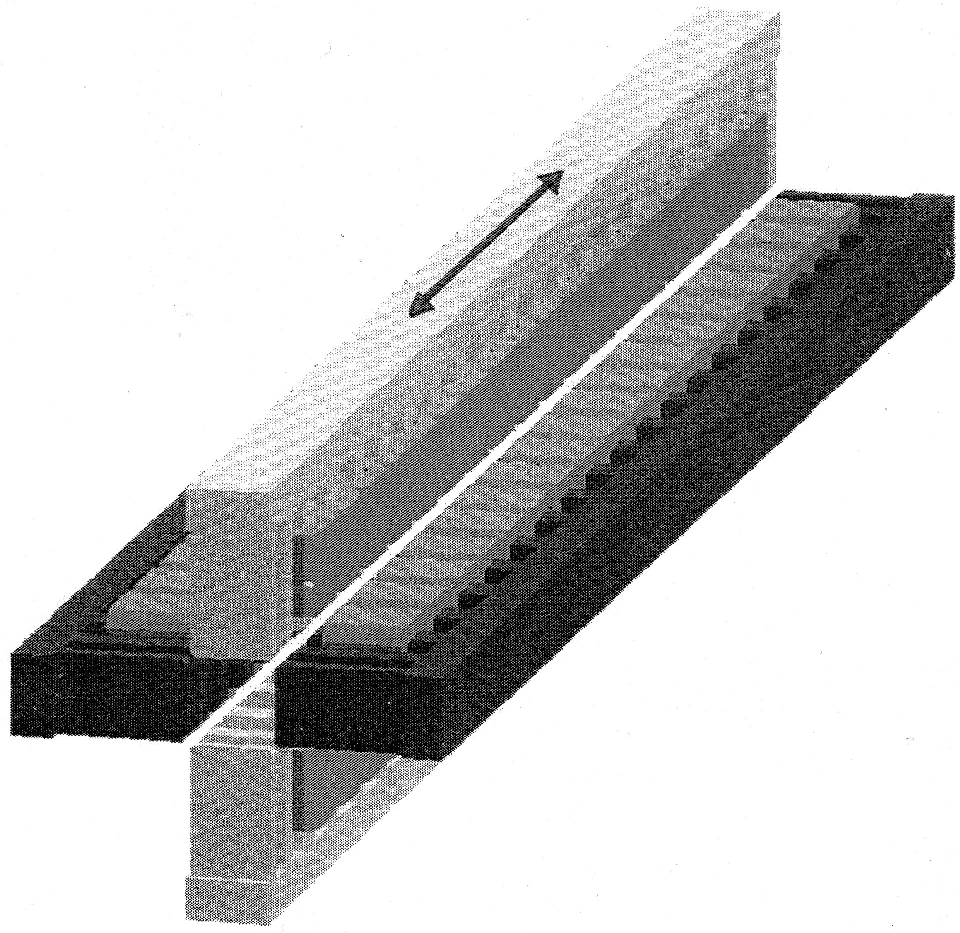
\includegraphics[width=0.4\columnwidth]{Figures/Soleil/onduleur.jpg}%
%%\caption{Schéma de l'onduleur croisé OPHELIE. Un onduleur peut être translaté par rapport à l'autre, permettant d'ajuster le déphasage entre les deux composantes de la lumière émise. Tiré de \mycite{NahonAO2004}.}
%%\label{fig:onduleur}
%%\end{figure}
%%
%%Pour la mesure de PECD, le polarimètre est retiré et le champ est envoyé dans la zone d'interaction du spectromètre VMI Delicious. Ce spectromètre est amélioré par rapport à celui présenté plus haut car il est capable de mesurer à la fois la distribution de vecteur vitesse des électrons et le temps de vol des ions créés par le champ VUV. Le temps de vol donne la masse des ions, ce qui permet d'effectuer une analyse de corrélation et de sélectionner les électrons provenant d'une espèce donnée. On résout également les différents rapports de branchement de l'espèce chirale, même si nous ne nous sommes pas encore intéressés à cette quantité.
%
%\subsection{Comparaison entre PECD en polarisation elliptique ou circulaire}
%%Commençons par étudier expérimentalement l'effet d'une polarisation elliptique sur la mesure de PECD. Comme expliqué plus haut, la polarisation du rayonnement synchrotron est modifiée en ajustant les paramètres de l'onduleur puis mesurée par le polarimètre VUV. On se place à une énergie de photon de 9.3 eV (énergie de la troisième harmonique dans la mesure réalisée au CELIA), et on choisit un rayonnement purement circulaire ou bien elliptique. Le champ elliptique a les paramètres de Stokes suivants :
%%\[ s_1=0.53\quad s_2=0.03\quad s_3=0.82, \]
%%ce qui correspond à une ellipse de polarisation tournée de $\eta=1.61$\degres~et d'ellipticité $\epsilon = 0.54$ (voir formules \ref{eq:stokes2inv}), tracée plus bas sur la figure \ref{fig:circ_ell_b0} .
 %%
%%On utilise un jet de fenchone (Sigma Aldrich). \`{A} cette énergie de photon, seule l'orbitale HOMO, d'énergie 8.6 eV, peut être ionisée. La figure \ref{fig:circ_ell_b0} présente le $b_0$ (spectre de photoémission) obtenu avec le rayonnement circulaire et elliptique. Le traitement utilise ici l'agorithme pBasex. L'échelle horizontale utilisée est l'énergie d'ionisation, définie comme $E_I = \hbar\omega - E_{\text{\'electron}}$. Les profils de $b_0$ sont remarquablement similaires. Leur amplitude est légèrement différente mais on rappelle que, pBasex ayant été utilisé, la valeur absolue de $b_0$ n'est pas correcte dans le cas elliptique.
%%
%%\begin{figure}[!ht]
%%\centering
%%\def\svgwidth{0.8\columnwidth}
%%\import{Figures/Soleil/}{Circ_Ell_b0.pdf_tex}
%%\caption{Mesures de $b_0$ dans la fenchone réalisées sur la ligne DESIRS à une énergie de photon de 9.3 eV. En traits pleins, polarisation circulaire. En pointillés, polarisation elliptique. Les deux ellipses de polarisation correspondantes sont tracées à droite de la figure.}
%%\label{fig:circ_ell_b0}
%%\end{figure}
%%
%%Sur la figure \ref{fig:circ_ell_b1} est représenté le paramètre dichroïque $b_1$ dans les cas circulaire et elliptique. On étudie ici la valeur de $b_1$ non normalisée par $b_0$, c'est-à-dire la simple différence $I^1-I^{-1}$. Les données pour le cas circulaire ont été prises dans la fenchone (+), tandis que celles du cas elliptique dans la fenchone (-). On a donc tracé $-b_1^{\text{circ}}$ et $b_1^{\text{ell}}$. En changeant d'énantiomère, on doit normalement mesurer une inversion parfaite de $b_1$. Au cours de cette campagne, nous avons observé une différence systématique entre les deux énantiomères. Une étude plus poussée, qui fait l'objet de l'article \ref{pap:NahonPCCP2016} \mycite{NahonNagGarciaEtAl2016}, a montré que cette différence était due à une différence de pureté énantiomérique des échantillons. Si l'échantillon de fenchone (+) était énantiopur à 99\%, celui de fenchone (-) ne l'était qu'à 82\%. Dans cette étude nous démontrons la possibilité de mesurer l'excès énantiomérique grâce au PECD avec une précision de $\pm1$\%. $b_1^{\text{ell}}$ ainsi que toutes les autres données dans la fenchone (-) ont donc été corrigées en fonction.
%%
%%\begin{figure}[!ht]
%%\centering
%%\def\svgwidth{0.8\columnwidth}
%%\import{Figures/Soleil/}{Circ_Ell_b1.pdf_tex}
%%\caption{Mesures de $b_1$ dans la fenchone (-) pour des polarisations circulaires et elliptiques. Les barres d'erreurs sont issues d'une analyse statistique.}
%%\label{fig:circ_ell_b1}
%%\end{figure}
%%
%%On voit que là où le signal est significatif (entre $\simeq8.5$ et $\simeq 9$ eV), les deux courbes de $b_1$ sont très ressemblantes, à un facteur de proportionnalité près. Sur la largeur à mi-hauteur du pic, on mesure $b_1^{\text{ell}}/b_1^{\text{circ}} = 0.83 \pm 0.03$. Rappelons qu'on a mesuré $s_3^{\text{ell}} = 0.82$ et que la ligne fournit en moyenne $s_3^{\text{circ}} \simeq 1$. Le PECD évoluant linéairement en $s_3$, on s'attend donc à une valeur théorique de $b_1^{\text{ell}}/b_1^{\text{circ}} \simeq 0.82$, ce qui est tout à fait dans notre intervalle de confiance. Nous avons donc vérifié expérimentalement la dépendance du PECD pour une polarisation imparfaite telle que celle du rayonnement harmonique.
%
%\subsection{Mesures de $b_1$ aux énergies harmoniques}
%%Nous présentons ici les mesures réalisées aux énergies correspondant aux harmoniques de la source présentée à la partie \ref{sec:sf6ghoe} : 9.3 eV (H3), 15.5 eV (H5) et 21.7 eV (H7). Nous avons également mesuré le PECD de la fenchone aux énergies correspondant à H4 et H6, ainsi que dans la zone 9.3 à 11.5 eV. Ces mesures, non présentées ici, serviront de données de référence pour de futures expériences dans lesquelles on prévoit d'observer des dynamiques vibrationnelles grâce au PECD résolu en temps.
%%
%%\begin{figure}[!ht]
%%\centering
%%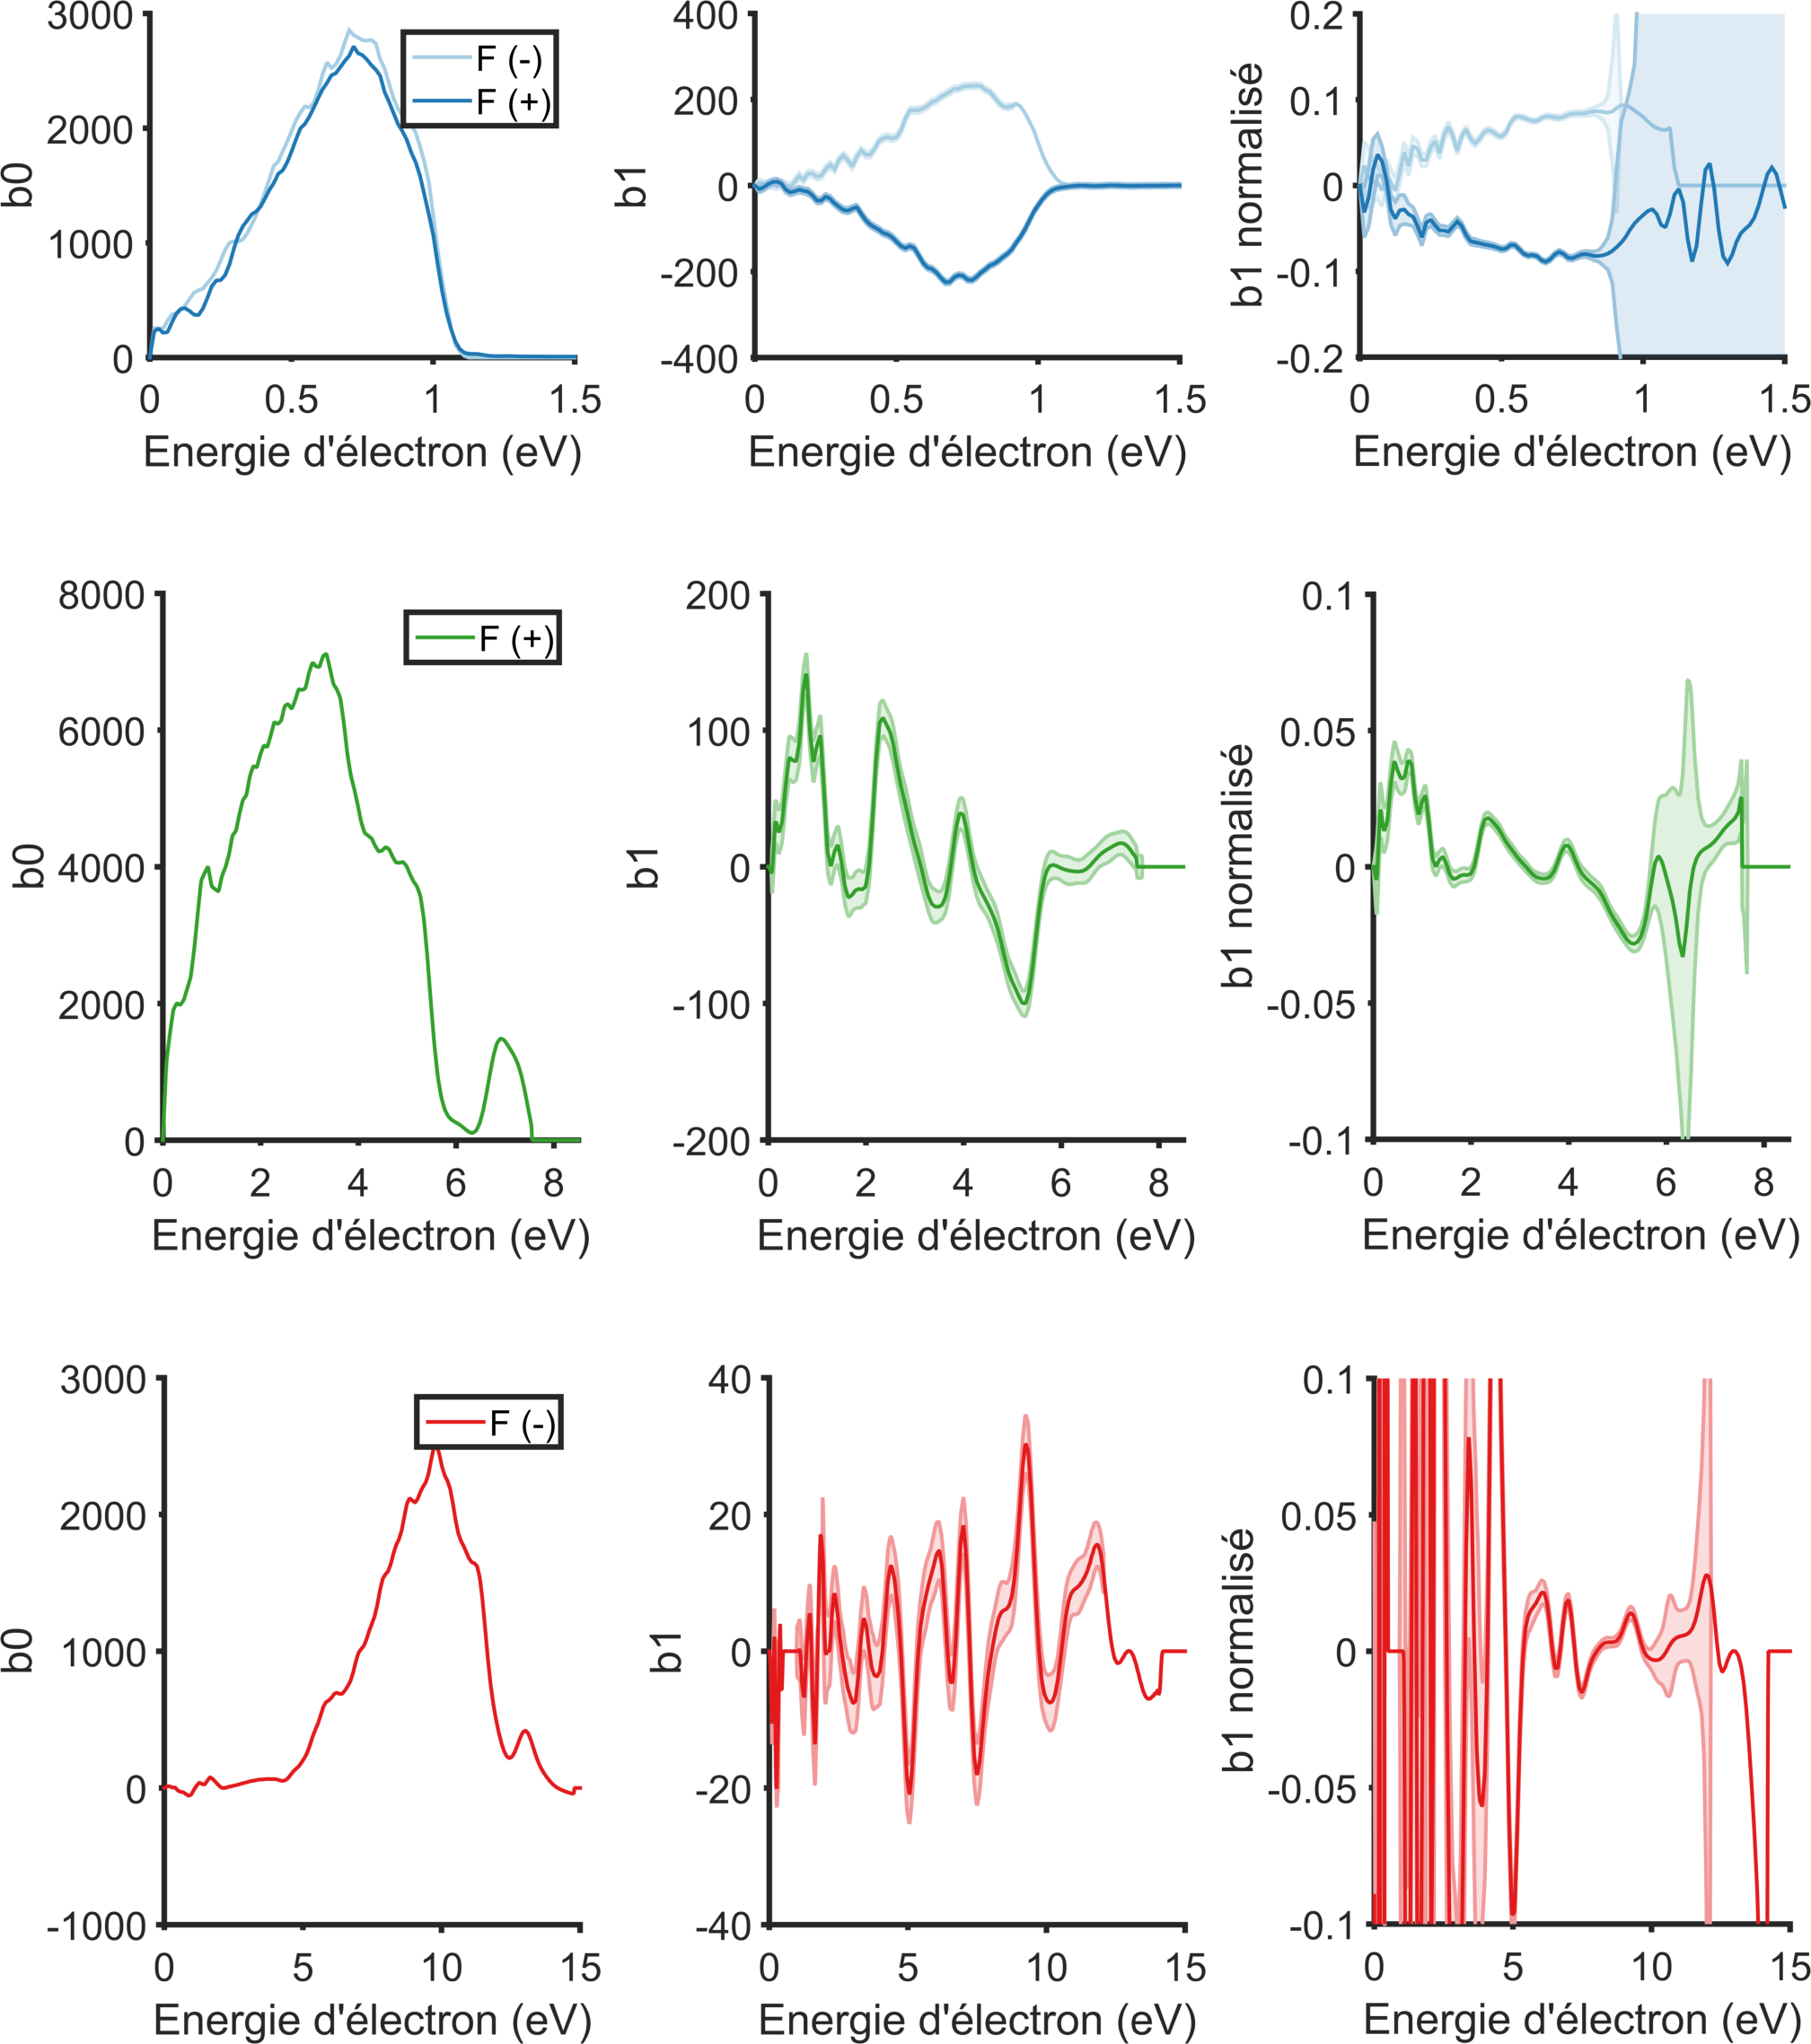
\includegraphics[width=1\columnwidth]{Figures/Soleil/Results_PECD.pdf}%
%%\caption{Résumé des mesures de PECD réalisées sur la ligne DESIRS. De gauche à droite : $b_0$ (spectre de photoémission), $b_1$, et $b_1$ normalisé par $b_0$. De haut en bas, énergies de photon égales à 9.3 eV, 15.5 eV et 21.7 eV. Pour la première énergie on a tracé la mesure pour les deux énantiomères.}
%%\label{fig:results_pecd}
%%\end{figure}
%%
%%Dans la figure \ref{fig:results_pecd}, on trace $b_0$, $b_1$, et $b_1/b_0$ pour les trois énergies harmoniques et pour un ou deux énantiomère. La polarisation étant ici complètement circulaire, l'utilisation de pBasex est justifiée. Quand on augmente l'énergie de photon, l'énergie maximale de photoélectron observée augmente également. Dans tous les cas, on observe clairement l'ionisation depuis la HOMO, à une énergie égale à $\hbar\omega-I_P^\text{HOMO}$, c'est-à-dire $\simeq \SI{0.7}{eV},\; \SI{6.9}{eV},\text{ et }\SI{13.1}{eV}$ respectivement pour H3, H5 et H7. Pour les énergies de photons plus élevées, la contribution d'orbitales plus basses apparaît. Les énergies de ces orbitales sont de plus en plus proches, et leurs contributions sont sommées dans le $b_1$ observé. $b_1$ est différent pour chacune d'entre elles et peut changer de signe, ce qui explique les profils riches observés dans cette région. Précisons pour terminer qu'à cause de problèmes de calibration en énergie aux hautes énergies de photon, certaines courbes ont été interpolées pour être cohérentes avec potentiels d'ionisation des différentes orbitales publiés dans la littérature \mycite{PowisCPC2008}.
%%\newpage
%\section{Comparaison entre mesures synchrotron et harmoniques}
%\label{sec:soleil_vs_celia}
%\subsubsection{Formulation mathématique}
%%Nous dispose désormais des données synchrotron nécessaires à la caractérisation complète de l'état de polarisation du champ harmonique. Toutefois, nous allons voir que nos mesures harmoniques sont incomplètes. Nous illustrerons ici le principe à suivre mais nous pourrons pas donner de véritable valeurs numériques en l'état.
%%
%%On considère donc le spectre constitué des 3 première harmoniques du fondamental à 400 nm. Quand il ionise la molécule de fenchone, on observe un spectre de photoémission qui est la somme de la contribution de chaque harmonique :
%%\[ b^{\text{GHOE}}_0(E) = \sum_{q={3,5,7}} s^{\text{GHOE},q}_0 \times b^{\hbar\omega=E_q}_0(E),\]
%%où $E_q$ et $s^{\text{GHOE},q}_0$ sont respectivement l'énergie et le $s_0$ (= l'intensité) de la q-ième harmonique.
%%
%%Les trois mesures synchrotrons donnent quant à elles pour $q=3,5,7$ :
%%\[ b^{\text{Sync},q}_0(E) =  s^{\text{Sync},q}_0 \times b^{\hbar\omega=E_q}_0(E),\]
%%
%%Notons les inconnues du problème $a_q = s^{\text{GHOE},q}_0/s^{\text{Sync},q}_0$ pour $q=3,5,7.$ On les obtient par un calcul d'ajustement, par exemple au sens des moindres carrés :
%%\begin{equation}
%%\min_{a_q} \sqrt{\int_{E=0}^{E_\text{max}} \left(b^{\text{GHOE}}_0(E)-\sum_{q={3,5,7}} a_q \times b^{\text{Sync},q}_0(E)\right)^2\rmd E}.
%%\label{eq:minb0}
%%\end{equation}
%%
%%La figure \ref{fig:sumb0} présente le profil de $\sum_{q={3,5,7}} b^{\text{Sync},q}_0(E)$, en utilisant les $b_0$ mesurés à la partie précédente (voir figure \ref{fig:results_pecd}). Elle permet de voir les régions dans lesquelles contribuent chaque énergie de photon.
%%
%%\begin{figure}[!ht]
%%\centering
%%\def\svgwidth{0.8\columnwidth}
%%\import{Figures/Soleil/}{sumPES.pdf_tex}
%%\caption{Sommes des $b_0$ mesurés au synchrotron à chaque énergie harmonique, en les supposant chacun normalisés et de poids égal.}
%%\label{fig:sumb0}
%%\end{figure}
%%
%%De la même manière, le paramètre dichroïque $b_1$ s'écrit pour les harmoniques :
%%\[ b^{\text{GHOE}}_1(E) = \sum_{q={3,5,7}} s^q_3 s^{\text{GHOE},q}_0 \times b^{\hbar\omega=E_q}_1(E),\]
%%et pour les mesures synchrotron, où on considère $s_3=1$ :
%%\[ b^{\text{Sync},q}_1(E) =  s^{\text{Sync},q}_0 \times b^{\hbar\omega=E_q}_1(E).\]
%%
%%La quantité à minimiser en fonction des trois inconnues $s_3^3,\;s_3^5,\;s_3^7$ est alors :
%%\begin{equation}
%%\min_{s_3^q} \sqrt{\int_{E=0}^{E_\text{max}} \left(b^{\text{GHOE}}_1(E)-\sum_{q={3,5,7}} s^q_3 \times a_q \times b^{\text{Sync},q}_1(E)\right)^2\rmd E}.
%%\label{eq:minb1}
%%\end{equation}
%%
%%En pratique, on minimise à la fois les problèmes \ref{eq:minb0} et \ref{eq:minb1} :
%%\begin{equation}
%%\min_{a_q,\;s_3^q} \sqrt{
	%%\begin{aligned}
	%%\int_{E=0}^{E_\text{max}}&\alpha_0\left(b^{\text{GHOE}}_0(E)-\sum_{q={3,5,7}} a_q \times b^{\text{Sync},q}_0(E)\right)^2 \\
	%%&+ \alpha_1\left(b^{\text{GHOE}}_1(E)-\sum_{q={3,5,7}} s^q_3 \times a_q \times b^{\text{Sync},q}_1(E)\right)^2	\rmd E
	%%\end{aligned}
	%%}
%%\label{eq:min_total}
%%\end{equation}
%%où $\alpha_0$ et $\alpha_1$ sont les poids relatifs qu'on donne arbitrairement à l'ajustement du $b_0$ et du $b_1$. Cette procédure donnera la valeur optimale de $s_3^3,\;s_3^5$ et $s_3^7$, valeurs inaccessible par des méthodes optiques.
%
%\subsubsection{Première application de la méthode}
%%Pour les données synchrotron, nous choisissons d'utiliser la mesure sur la fenchone (+) pour H5, et sur la fenchone (-) pour H3 et H7 où on inversera le $b_1$. Ces mesures sont les plus précises du fait d'un très bon niveau de signal, et ne présentent pas de problème de calibration. On prend également soin de corriger les mesures dans la fenchone (-) de l'erreur due à l'excès énantiomérique inférieur à 1.
%%
%%Pour les données harmoniques, les seules dont nous disposons actuellement sont celles présentées sur la figure \ref{fig:pecdfenchone}. Le problème est qu'elles ont été obtenues par application de l'algorithme pBasex, qui introduit un artefact pour une polarisation non circulaire. On peut toujours étudier le $b_1$ non normalisé par $b_0$ (c'est-à-dire la différence directe entre les deux images), mais la formule \ref{eq:min_total} montre bien la nécessité de connaître $b_0$ pour comparer les deux mesures.
%%
%%En plus de ce problème d'analyse, ces données ne sont pas parfaites : des zones du détecteurs étaient brûlées (visible sur la figure \ref{fig:pecdfenchone} vers 6 eV), et un bruit de fond n'a pas été correctement soustrait. Nous appliquerons donc le calcul présenté plus haut tout en gardant à l'esprit que les valeurs finales seront incorrectes. 
%%
%%Le problème \ref{eq:min_total} est résolu au sens des moindres carrés par un algorithme à région de confiance réflectif \mycite{BranchColemanLi1999}. On restreint de plus le domaine d'énergie sur lequel on minimise la fonction, de sorte à ne garder que les pics significatifs. $b_1$ étant le paramètre qui nous intéresse le plus, on choisit des facteurs de pondération $\alpha_1/\alpha_0 = 100$. La figure \ref{fig:results_minim_P} illustre le résultat de l'algorithme, qui converge en quelques dizaines d'itérations, pour la fenchone (+). Les $b_1$ des mesures synchrotrons sont ensuite inversés pour analyser le cas de la fenchone (-), illustré sur la figure \ref{fig:results_minim_M}.
%%
%%\begin{figure}[!ht]
%%\centering
%%\def\svgwidth{0.75\columnwidth}
%%\import{Figures/Soleil/}{results_minim_P.pdf_tex}
%%\caption{Détermination des $s_3$ harmoniques par comparaison avec les données synchrotron dans la fenchone (+). En traits pleins bleus, résultats de l'algorithme de minimisation. En pointillés rouges, mesures faites avec la source d'harmoniques d'ordre élevé. Les rectangles verts illustrent le domaine d'énergie où a été effectuée la minimisation. Les valeurs de $s_3$ obtenues sont indiquées.}
%%\label{fig:results_minim_P}
%%\end{figure}
%%
%%\begin{figure}[!ht]
%%\centering
%%\def\svgwidth{0.75\columnwidth}
%%\import{Figures/Soleil/}{results_minim_M.pdf_tex}
%%\caption{Détermination des $s_3$ harmoniques par comparaison avec les données synchrotron dans la fenchone (-). En traits pleins bleus, résultats de l'algorithme de minimisation. En pointillés rouges, mesures faites avec la source d'harmoniques d'ordre élevé. Les rectangles verts illustrent le domaine d'énergie où a été effectuée la minimisation. Les valeurs de $s_3$ obtenues sont indiquées.}
%%\label{fig:results_minim_M}
%%\end{figure}
%%
%%On note tout d'abord un accord très satisfaisant sur le $b_1$. Ceci démontre la possibilité d'effectuer des mesures précises de PECD avec une source harmonique. L'accord sur le $b_0$ est moins bon, du fait du choix d'un $\alpha_0\ll\alpha_1$. Les valeurs de $s_3$ obtenues sont précisées sur les figures. Précisons encore une fois que ces valeurs ne sont pas correctes à cause des artefacts sur $b_0$ introduits par l'utilisation de pBasex et les défauts expérimentaux. Ce point est bien visible puisque les valeurs de $s_3^5$ et $s_3^7$ diffèrent entre les deux énantiomères, alors que la source est restée la même entre les deux expériences.\par
%%Toutefois, nous montrons ici la possibilité de réaliser une caractérisation de l'état de polarisation du rayonnement. Pour l'obtenir complètement (ellipticité, dépolarisation, angle de l'ellipse), il faudrait en plus connaître les $s_1$ et $s_2$. Une nouvelle campagne d'expérience est prévue au CELIA Bordeaux, dans laquelle on réalisera les mesures pour l'instant manquantes :
%%
%%
%%\begin{itemize}
%%\renewcommand{\labelitemi}{$\bullet$}
%%\setlength\itemsep{1em}
%%\item Les données seront cette fois analysées par une autre méthode, en prenant en compte la polarisation elliptique du rayonnement. On obtiendra alors la véritable valeur de $b_0$, permettant de déterminer les $a_q$ correctement.
%%\item Le détecteur du VMI a été remplacé et ne présente plus de dommage.
%%\item Un polarimètre a été installé juste après le VMI. Il permet de réaliser des loi de Malus et de mesurer $s_1$, $s_2$, et la borne supérieure $s_3^{\text{max}}$. Il est également adapté à la mesure des paramètres de la troisième harmonique, ce qui n'était pas le cas jusqu'à présent (voir figure \ref{fig:sf6_ell}). Les mesures de PECD et de loi de Malus seront effectuées dans des conditions identiques, ce qui permettra de déterminer $\eta$, $P$, et $\epsilon$. 
%%\end{itemize}
%
%\chapternonum{Conclusion et perspectives}
%%Dans cette partie, nous avons d'abord développé une source d'harmoniques d'ordre élevé polarisées elliptiquement. En plus du contrôle du moment angulaire orbital, démontré à la partie précédente, nous contrôlons ici le moment angulaire de spin dans le domaine ultraviolet. En tant qu'objet chiral, la lumière polarisée circulairement est sensible à la chiralité de molécules, ce que nous avons démontré en effectuant des mesures de dichroïsme circulaire de photoélectron. Nous avons réalisé ces mêmes mesures sur un synchrotron, source de lumière parfaitement caractérisée. La comparaison entre les deux montre d'abord que les deux sources donnent des mesures spectroscopiques comparables. Nous avons ensuite étudié la possibilité de caractériser l'état de polarisation de notre source harmonique grâce au PECD.

%% We want the conclusion at the part level in the table of content but look like a chapter
% -> we shift the toclevel of everything
%\makeatletter
%\def\toclevel@chapter{-1}
%\def\toclevel@section{0}
%\def\toclevel@subsection{1}
%\makeatother

% we also want the numbering to start back at A
\renewcommand{\thesection}{\Roman{section}}
\setcounter{section}{0}
%it is going to mess hyperref links because it will have the same name as previous sections -> we change it
\renewcommand*{\theHsection}{CL.\the\value{section}}
% same for figures
\renewcommand{\thefigure}{\Roman{section}.\arabic{figure}}
\setcounter{figure}{0}


\chapternonumtoc{Conclusions et Perspectives}

Nous avons étudié le comportement des deux types de moment angulaire dans la génération d'harmonique d'ordre élevé. Nous avons pu observer sa conservation, ce qui soutient la représentation de la GHOE comme un processus paramétrique. Cela permet également de transférer ces propriétés au rayonnement harmonique, c'est-à-dire à des impulsions ultra-brèves de très courte longueur d'onde. Dans ce chapitre de conclusion, nous récapitulons ces résultats et présentons les développements envisagés à partir de ces sources de lumière uniques. Nous discuterons successivement des deux composantes du moment angulaire de la lumière.

\section{Perspectives d'utilisation de rayonnement XUV portant du moment angulaire orbital}
Dans la partie \ref{CH:OAM_HHG}, nous avons d'abord discuté de la génération d'harmoniques d'ordre élevé à partir d'un faisceau de Laguerre-Gauss. Cette expérience s'ajoute à deux précédentes \mycite{ZurchNP2012,GariepyPRL2014} et étend l'étude du transfert de MAO à une gamme de paramètre bien plus large. Le moment angulaire orbital porté par le rayonnement harmonique a été caractérisé en utilisant les propriétés de divergences des faisceaux de Laguerre-Gauss, qui permet d'obtenir la loi de transfert $\ell_q=q\times\ell_1$ attendue théoriquement \mycite{HernandezPRL2013}. Contrairement aux études précédentes, qui utilisent une méthode de caractérisation directe, notre raisonnement se base uniquement sur une observation du profil d'intensité harmonique en champ lointain. Il s'appuie sur des calculs analytiques et numériques (chapitre \ref{sec:OAM_analysis}) et sur le fait que dans un processus non-linéaire, les maxima du champ émis au foyer coïncident avec ceux du champ de génération, qui est lui bien caractérisé. Cette approche indirecte est applicable quelque soit la longueur d'onde générée, ce qui nous a permis d'étudier les cas où le laser de génération porte $\ell_1=1$, $2$ ou $3$ unités de MAO. La plus haute valeur de MAO harmonique est obtenue pour $\ell_1=3$, où $\ell_{19} = 57$. Nous avons également pu étendre l'étude à des longueurs d'ondes très courtes, jusqu'à $\lambda_{41} = 19.5$ nm, en utilisant le néon comme gaz de génération.

\subsection{Génération de moment angulaire orbital arbitraire}
Ces résultats nous amènent à envisager des applications utilisant ce rayonnement aux propriétés particulière. Dans un premier temps, il serait toutefois souhaitable de disposer d'un rayonnement XUV portant de faibles valeurs de MAO. Le schéma direct présenté ici n'est pas très flexible puisque gouverné par la loi $\ell_q=q\times\ell_1$. Pour répondre à ce problème, nous avons implémenté un schéma à deux faisceaux non-colinéaires, initialement proposé par \mycite{GariepyPRL2014}. On y utilise un faisceau à 800 nm Gaussien qui croise un faisceau à 400 nm portant $\ell_1 = 1$ dans la zone d'interaction avec le jet de gaz. Ce dispositif est très similaire à celui présenté à la partie \ref{sec:calib} et se comprend dans une image photonique : l'harmonique d'ordre $q$ peut être générée par l'absorption de $q$ photons rouges, mais également de $q-4n$ photons rouges et $2n$ photons bleu. Le faisceau bleu étant non-colinéaire, la contribution du chemin $(q-4n,2n)$ sera décalée en champ lointain à mesure que $n$ augmente. De plus, le faisceau bleu portant $\ell_1=1$, la conservation du MAO impose que la contribution du chemin $(q-4n,2n)$ porte un MAO égal à $2n$. Ainsi, on peut générer à une longueur d'onde quelconque des faisceaux portant des valeurs très faibles de MAO.

Cette expérience a été réalisé à l'université de Nova Gorica, en collaboration avec le groupe de Prof. G. De Ninno. Nous présentons des résultats préliminaires sur la figure \ref{fig:gauthier}, où on observe le spectre harmonique en champ lointain. 

\begin{figure}[!ht]
\centering
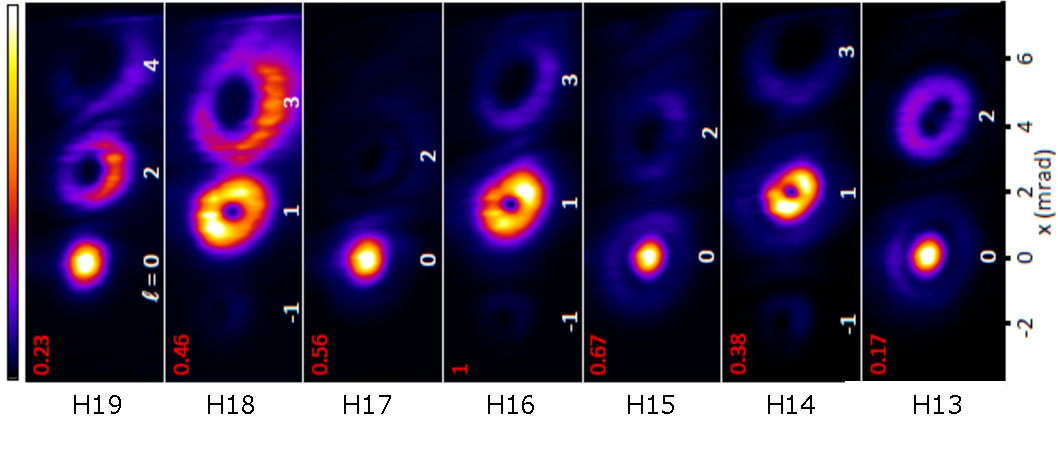
\includegraphics[width=0.8\columnwidth]{Figures/Conclusion/gauthier.pdf}%
\caption{Intensité en champ lointain obtenue à partir du schéma à deux couleurs non-colinéaires. Chaque mode est repéré par le nombre de photons bleus absorbés, c'est-à-dire par leur moment angulaire orbital.}
\label{fig:gauthier}
\end{figure}
Pour chaque harmonique, on observe de nombreux ordres de diffractions portant des valeurs de MAO différentes. Ces valeurs ont été confirmées par une mesure de front d'onde à l'aide d'un capteur de Hartmann, capable de résoudre la phase hélicoïdale pour ces faibles valeurs de $\ell$.

\subsection{Des impulsions attosecondes couplées spatio-temporellement : les light springs}
Dans un second temps, nous avons présenté une caractérisation complète du train d'impulsion attoseconde généré à partir d'un faisceau de Laguerre-Gauss. Pour ce faire, nous avons utilisé la technique RABBIT, qui permet de mesurer la phase relative entre chaque harmonique constituant le train d'impulsions. Ces mesures ont mis en évidence un problème intéressant : dans la technique RABBIT, le signal mesuré est intégré sur la totalité du volume d'interaction. Si on utilise une impulsion attoseconde portant du MAO et une impulsion d'habillage Gaussienne, la phase entre les deux faisceaux varie entre 0 et $2\pi$ dans le volume et la somme cohérente de ces contributions donne un résultat nul : les pics satellites de la trace RABBIT n'oscilleront pas. Nous avons donc utilisé une impulsion d'habillage portant le même MAO que celle de génération, de sorte à avoir un accord parfait entre les deux faisceaux au sein de la zone d'interaction. Il s'agit à notre connaissance de la première mesure de phase spectrale pour un faisceau non-Gaussien.

\subsubsection{Mesures de phase spectrale résolues spatialement}
Il est communément supposé que la phase spectrale varie peu selon les coordonnées spatiales, principalement car cette variation ne peut être résolue. En vérité, de nombreuses inhomogénéités peuvent introduire des couplages \textit{spatio-temporaux} dès l'impulsion laser de génération. On se reportera à la thèse de Gustave Pariente pour une discussion très complète sur la caractérisation de ces couplages dans le domaine infrarouge. Ils sont bien sûr transmis et amplifiés dans la GHOE, ce qui enlève une grande part de validité aux mesures intégrées spatialement. Un des axes principaux de recherche dans le domaine de la GHOE est la production d'impulsion attoseconde très énergétique, à partir de lasers de génération intenses qui interagissent sur plusieurs centimètres avec le milieu gazeuse. Il est très probable que dans ces régimes extrêmes, les couplages spatio-temporaux dans l'XUV seront un facteur limitant à l'augmentation de l'intensité sur cible.

Nos résultats suggèrent que la technique RABBIT habituelle pourrait être modifiée pour obtenir une partie de ces informations \textit{spectro-spatiales}. En effet, nous avons mis en évidence la possibilité de modifier le faisceau d'habillage pour avoir accord ou non avec le faisceau harmonique. Plutôt que d'accorder habillage et génération sur tout le volume, on pourrait restreindre de manière contrôlée la zone d'accord de sorte à mesurer la phase spectrale provenant seulement de cette partie du faisceau. Pour ce faire, il est plus simple d'utiliser l'intensité que la phase : si on utilise un faisceau d'habillage plus petit spatialement, seule la zone où les intensités des deux faisceaux sont nulles contribuera à la trace RABBIT. 

Nous avons réalisé des expériences préliminaires pour tester ce principe, dans le cadre d'une collaboration avec le groupe de Prof. L.F. DiMauro de la Ohio State University (Columbus OH, USA). Comme cas test, on cherche à caractériser un mode de Laguerre-Gauss XUV, pour lequel la phase varie linéairement avec la coordonnée azimutale. Pour le faisceau d'habillage, nous avons utilisé une lame de phase présentant une marche de $\pi$ \mycite{CamperPRA2014}. Cette lame crée au foyer deux tâches focales séparées de $\sim \SI{100}{\micro\metre}$, comme représenté sur la figure \ref{fig:spatialrabbit}. 

\begin{figure}[!ht]
\centering
\def\svgwidth{\columnwidth}
\import{Figures/Conclusion/}{spatial_rabbit.pdf_tex}
\caption{Principe d'une expérience RABBIT résolue spatialement. Le faisceau de génération (a) donne un profil de LG aux harmoniques générées. Le faisceau d'habillage (b) présente deux tâches focales, séparées d'une distance similaire au diamètre de l'anneau de génération. Ce profil peut être tourné d'un angle noté $\theta$. (c) La contribution à la mesure RABBIT est déterminée par le recouvrement entre ces deux profils d'intensité. (d) Pour chaque valeur de $\theta$, on mesure les oscillations des pics satellites dans la trace RABBIT. La phase de ces pics satellites nous donne $\phi_q(\theta)$.}
\label{fig:spatialrabbit}
\end{figure}

Si le faisceau d'habillage (\ref{fig:spatialrabbit}.b) est ajusté pour avoir une taille similaire à l'anneau du faisceau de génération (\ref{fig:spatialrabbit}.a), on peut limiter la zone contribuant à la mesure RABBIT (\ref{fig:spatialrabbit}.c). La lame de phase $0-\pi$ est montée sur une rotation motorisée, permettant de sélectionner l'angle contribuant à la trace RABBIT. Pour chaque valeur de cette angle $\theta$, on mesure les oscillations à 2$\omega$ des pics satellites. La phase de ces oscillations donne donc la phase spectrale résolue angulairement, $\phi_q(\theta)$. La figure (\ref{fig:spatialrabbit}.d) illustre le décalage entre $\theta_1$ et $\theta_1+\pi/2$ pour une phase quelconque. Pour un faisceau de Laguerre-Gauss idéal de moment $\ell_q$, on s'attend à mesurer $\phi_q(\theta) = \ell_q\theta+2\Delta t_e\omega_q$, où $\Delta t_e$ est le temps d'émission de l'atome de détection utilisé. Ces expériences n'ont pour l'instant pas été conclues, mais ce principe pourrait être généralisé à des mesures spatiales selon d'autres coordonnées.

\subsubsection{Utilisation du couplage spatio-temporel en physique ultra-rapide}
Les mesures RABBIT réalisées nous ont permis de reconstruire complètement le profil spatio-temporel du train attoseconde généré. Dans le cas de faisceaux portant du MAO, on obtient un profil d'intensité très particulier à deux spirales imbriquées. Cela met en évidence un couplage spatio-temporel très fort, où l'intensité est retardée temporellement avec la coordonnée azimutale. Nous discutons ici des possibilités d'utiliser les couplages spatio-temporels des faisceaux de LG en physique ultra-rapide.

Comme on l'a mentionné, les couplages spatio-temporels sont souvent non désirables en physique des champs forts. Toutefois, \mycite{VincentiPRL2012} ont montré qu'ils pouvaient aussi être introduits volontairement pour contrôler l'émission harmonique. Dans leur schéma, on utilise un prisme cale (\textit{wedge} en anglais) pour introduire une rotation de front d'onde au foyer au cours du temps, qui émet chaque impulsion attoseconde selon une direction angulaire donnée. \linebreak
Un faisceau de Laguerre-Gauss, de par sa phase $\ell\theta$, présente également un couplage spatio-temporel. La phase en un point donné évolue entre 0 et $\ell 2\pi$ pendant un cycle optique, on peut donc l'utiliser pour observer des phénomènes sub-cycles. Nous illustrons cette possibilité en commençant par un faisceau de Laguerre-Gauss infrarouge.

Intéressons-nous à la génération d'harmonique à deux couleurs. Dans ce schéma, des harmoniques sont générées par un faisceau à 800 nm superposé à sa deuxième harmonique, à 400 nm. Cette seconde couleur brise la centro-symétrie de la GHOE, qui était responsable de la génération d'harmoniques impaires uniquement. On obtient donc un spectre composé des harmoniques paires et impaires du laser de génération. \mycite{DudovichNP2006} ont montré que quand le champ à 400 nm est très faible, il vient simplement perturber le phénomène de GHOE habituel : au cours de l'étape de propagation du modèle à trois étapes, la trajectoire électronique est légèrement modifiée. Une analyse perturbative montre qu'en changeant le délai entre les deux couleurs, il est possible de remonter au temps d'émission électronique, ainsi qu'aux paramètres $t_i$ et $\bm{p}$ du modèle SFA \mycite{PedatzurNP2015}. L'observable mesurée ici est l'intensité harmonique en fonction du délai rouge-bleu noté $\tau$. Elle s'écrit dans le cas perturbatif et si les polarisations des champs sont parallèles :
\begin{equation}
I_q(\tau)=
\begin{cases}
I_1 + I^q_0\left|\cos(\omega_{800}\tau+\phi_q)\right|^2\text{ si $q$ impair}\\
I_2 + I^q_0\left|\sin(\omega_{800}\tau+\phi_q)\right|^2\text{ si $q$ pair}
\end{cases}
\label{eq:oren}
\end{equation}
L'information à extraire est $\phi_q$, on peut donc effectuer un scan de délai entre les deux faisceaux (figure \ref{fig:rb_mapping}.a). Une autre approche est de paramétrer ce délai spatialement de sorte à ne pas avoir à faire de scan. Prenons par exemple des faisceaux rouges et bleus portant chacun $\ell=1$. Leur phase s'écrit au point $(r,\theta)$ :
\begin{align}
\varphi_{400}(r,\theta,t) &= \omega_{400}(t + \theta/\omega_{400}),\\
\varphi_{800}(r,\theta,t) &= \omega_{800}(t + \theta/\omega_{800}).
\end{align}
Le délai les séparant s'écrit donc en tout point $\tau(r,\theta) = \theta/\omega_{800}-\theta/\omega_{400} = \theta/\omega_{400}$, ce qui est tracé en \ref{fig:rb_mapping}.b. On a donc un délai variant spatialement : le délai rouge-bleu est paramétré sur la coordonnée azimutale. On retrouvera donc l'évolution temporelle de l'intensité des harmoniques sur leur coordonnée azimutale, comme illustré sur la figure \ref{fig:rb_mapping}.c.
\begin{figure}[!ht]
\centering
\def\svgwidth{\columnwidth}
\import{Figures/Conclusion/}{rb_lg_mapping.pdf_tex}
\caption{Principe d'expériences de GHOE à deux couleurs utilisant le couplage spatio-temporel des faisceaux de LG. L'expérience habituelle est de mesurer le spectre harmonique en fonction du délai rouge-bleu (a). Si on utilise des faisceaux de LG, on a un délai variant azimutalement (b). Les harmoniques générées sont donc modulées selon $\theta$, ce qui permet de mesurer $\phi_q$ sans effectuer de scan (lignes pointillées rouges).}
\label{fig:rb_mapping}
\end{figure}
Expérimentalement, les harmoniques sont observées en champ lointain. Nous ne pouvons pas réaliser le calcul de propagation car nous ne connaissons pas la phase spatiale des harmoniques, elle aussi perturbée par le champ à 400 nm. Nous prévoyons d'effectuer des calculs SFA 4D complets pour prédire et quantifier cet effet. Dans tous les cas, l'observable $\phi_q$ se retrouvera dans le profil spatial en champ lointain. On peut donc mesurer la quantité recherchée en un seul tir laser, plutôt qu'en effectuant un scan de délai.

Dans le cas de faisceaux de Laguerre-Gauss dans l'XUV, on a la même propriété de phase paramétrée avec l'angle. De plus, si on considère non plus une harmonique donnée mais l'impulsion attoseconde entière, l'intensité a un profil de \textit{light spring}. Chaque point de l'espace $(r,\theta)$ voit donc un train d'impulsion attoseconde qui se décale temporellement de façon linéaire avec $\theta$. Cette propriété pourrait être utilisée dans une expérience d'absorption transitoire, dans laquelle on mesure habituellement l'intensité transmise par un échantillon, intégrée spatialement, au cours du temps. Avec un light spring, on pourrait plutôt résoudre spatialement l'intensité transmise, dans laquelle chaque valeur de $\theta$ correspond à une valeur de délai différente.

\subsection{Spectroscopies utilisant le moment angulaire orbital XUV}
En plus de ces couplage spatio-temporels, les faisceaux de Laguerre-Gauss possèdent un intérêt plus fondamental : les photons y portent un moment angulaire orbital bien défini. Il est très tentant de voir cette grandeur comme un paramètre supplémentaire pour contrôler et étudier l'interaction laser-matière. Par exemple, la perspective de nouvelles règles de sélection en photoionisation suggère la possibilité d'étudier des niveaux atomiques normalement interdits. Dans la partie \ref{sec:selectionrules}, nous avons montré que la réalité n'était pas si clémente : le MAO se couple préférentiellement au moment externe d'un atome. Le couplage avec le moment interne de l'atome n'apparaît qu'au second ordre. C'est également ce qui est observé dans nos mesures RABBIT : si la photoionisation était modifiée par la présence de MAO, on aurait mesuré un temps d'émission différent de celui obtenu en faisceau gaussien\footnote{En effet, le temps d'émission dépend du niveau électronique ionisé. Par exemple, \mycite{SchultzeScience2010} ont mesuré un délai de 21 as entre les électrons issus de l'orbitale 2p du néon par rapport à ceux issus de la 2s.}.

Dans notre expérience, nous disposions d'un faisceau de diamètre $\sim \SI{100}{\micro\metre}$ au foyer, à comparer avec un atome d'argon dont le diamètre est de l'ordre de l'Angström. Là est le problème principal : à l'échelle de l'atome, la phase du faisceau de LG est plate. Il n'y a qu'au centre du faisceau que la phase varie à l'échelle de l'atome, mais l'intensité y est nulle. Une transition quadripolaire dépendant du gradient du champ électrique, il est naturel qu'on ne les observe pas  dans notre cas. Pour cette raison, l'intégralité des prédictions théoriques sont jusqu'à présent limitées à des valeur d'intensité et de focalisation non réalisables en pratique. Par exemple, \mycite{PiconOE2010} prédit une modification des règles de sélection pour l'atome d'hydrogène, avec un faisceau à 27.2 eV, de waist $\SI{4.79}{\micro\metre}$ et d'intensité égale à $\SI{6.8e18}{\W\per\centi\metre\squared}$. De même, \mycite{WatzelPRA2016} proposent une mesure de délais attosecondes de nouveaux niveaux atomiques dans l'argon à partir d'un faisceau à 90 eV et d'intensité $\SI{5.6e19}{\W\per\centi\metre\squared}$.

De telles intensités dans l'XUV dépassent l'état de l'art actuel de nombreux ordres de grandeurs. S'il est certain que les intensités XUV disponibles continueront d'augmenter dans le futur, il est sûrement plus simple de chercher des systèmes plus adaptés, c'est-à-dire plus gros par rapport au faisceau harmonique. Par exemple, un atome de Rydberg a un rayon déjà bien plus important : pour le niveau n=137 de l'hydrogène, il vaut $\sim\SI{1}{\micro\metre}$. D'autres candidats sont les agrégats d'atome, ou bien des molécules de $\text{C}_{60}$, un des plus gros objets dans lequel a été observée la dualité onde-particule \mycite{ArndtNat1999}. Leur interaction avec un faisceau portant du MAO est étudié par \mycite{WatzelPRA2016}, qui observent un effet pour une intensité de $\SI{3.2e17}{\W\per\centi\metre\squared}$. L'intensité est réduite par rapport à l'argon mais pas de manière suffisante pour envisager une expérience.\linebreak
Peut-être que les cibles adaptées aux capacités expérimentales actuelles ne doivent pas être cherchées parmi les molécules, mais plutôt dans la phase condensée. Il est en effet possible de créer optiquement des excitations collectives à la surface ou dans le volume d'un solide, dont certaines pourraient être sensibles au MAO. Deux propositions intéressantes existent en ce sens : \mycite{VanVeenendaalPRL2007} prédit un dichroïsme induit par le MAO dans l'absorption au point K de métaux de transitions, tandis que \mycite{VanVeenendaalPRB2015} discute de l'interaction entre un faisceau de LG XUV et un vortex magnétique. Nous sommes en train d'évaluer la faisabilité expérimentale de ces propositions.

En conclusion, il nous semble très intéressant de continuer à développer le contrôle de faisceaux harmoniques portant du moment angulaire orbital. Les utilisations les plus immédiates nous paraissent être celles utilisant les propriétés macroscopiques de ces faisceaux. Nous avons mentionné l'utilisation de la structure spatio-temporelle des modes de LG et des impulsions attosecondes générées, qui survit dans le cas d'impulsions attosecondes isolées \mycite{HernandezPRL2013}. Il serait également assez direct d'utiliser les faisceaux de LG XUV en imagerie. En effet, ils sont déjà utilisés dans le domaine visible pour la microscopie \mycite{FurhapterOL2005} et commencent à être étudiés pour l'imagerie par diffraction cohérente \mycite{wangOE2009}. La résolution de ces deux techniques est grandement améliorée par l'utilisation de rayonnement XUV; nos résultats permettent donc d'envisager la combinaison avantageuse de faibles longueurs d'ondes et de modes de LG. \linebreak
Quant aux applications d'impulsions attosecondes portant du MAO en spectroscopie, il est probablement trop tôt pour prédire la marche à suivre. L'étude théorique de l'interaction doit continuer à se développer en se dirigeant vers des conditions plus réalistes expérimentalement, tandis que la production expérimentale de faisceaux intenses et fortement focalisés doit être optimisée dans l'XUV. Mentionnons pour terminer une autre voie de recherche ouverte par de récentes propositions \mycite{RibiPRL2014,HemsingPRL2011,HemsingPRL2012}. Elles visent à contrôler le moment angulaire orbital de lasers à électron libre, qui fournissent un rayonnement XUV très intense. Nous avons eu la chance de participer aux premiers essais d'implémentation sur FERMI (Trieste, Italie) et tenons à remercier Prof. G. De Ninno et D. Gauthier pour cette opportunité.

\section{Conclusions et perspectives sur les mesures de dichroïsme circulaire de photoélectron}
Dans la partie \ref{PA:Spin_HHG}, nous avons étudié l'effet du moment angulaire de spin dans la génération d'harmoniques d'ordre élevé. Nous avons vu qu'il y est conservé, mais que l'efficacité du processus habituel chute fortement à mesure que l'ellipticité du laser de génération augmente. Nous avons étudié la GHOE au voisinage d'une résonance du milieu de génération, dans le cas d'une résonance près du seuil de l'argon, et d'une résonance de forme dans le continuum d'une molécule, ici \sf6. Aux énergies résonantes, on observe une forte augmentation de l'ellipticité harmonique attribuée à une modification de la dynamique électronique au moment de la recombinaison. Cette interprétation est soutenue par des calculs TDSE, réalisés par B. Pons et B. Fabre. 

\subsection{GHOE proche du seuil de l'argon : l'effet xFID}
Dans le cas particulier de l'argon, ces expériences ont mis en évidence le phénomène de xFID. Il a été étudié en détail par \mycite{beaulieuArXiv2016}. En collaboration avec Samuel Beaulieu, \'{E}tienne Bloch, Valérie Blanchet et Yann Mairesse, nous avons poursuivi ces expériences en utilisant une longueur d'onde de 400 nm et en choisissant des conditions de focalisation favorisant grandement le xFID. Dans ce processus, on crée une superposition cohérente entre l'état fondamental et plusieurs états de Rydberg de l'atome. Le paquet d'onde ainsi créé se désexcite en émettant un rayonnement XUV cohérent. Cette technique est très proche de l'absorption transitoire attoseconde (ATAS, pour \textit{Attosecond Transient Absorption Spectroscopy}) \mycite{BeckNJP2014}, dans laquelle les oscillations d'un dipôle induit par une excitation XUV sont observées à l'aide d'une seconde impulsion infrarouge. Il est possible de réaliser une expérience pompe-sonde similaire en perturbant l'émission xFID à l'aide d'une impulsion infrarouge de délai variable. Des expériences préliminaires démontrent la possibilité de résoudre les battements femtoseconde du paquet d'onde électronique créé dans l'argon. \`A ces mesures d'amplitude nous prévoyons d'ajouter une mesure de phase en utilisant la technique d'interférométrie à deux sources développée par \mycite{CamperThesis2014}. Dans cette technique, on crée deux sources de xFID séparées spatialement qui interfèrent en champ lointain. En perturbant une seule des deux sources avec une impulsion infrarouge, on retrouve le déphasage induit dans ces interférences spatiales. La figure \ref{fig:xfid_deuxsources} présente un exemple de franges observées à l'aide de ce dispositif. Ces expériences sont toujours en cours au CELIA Bordeaux. 

\begin{figure}[!ht]
\centering
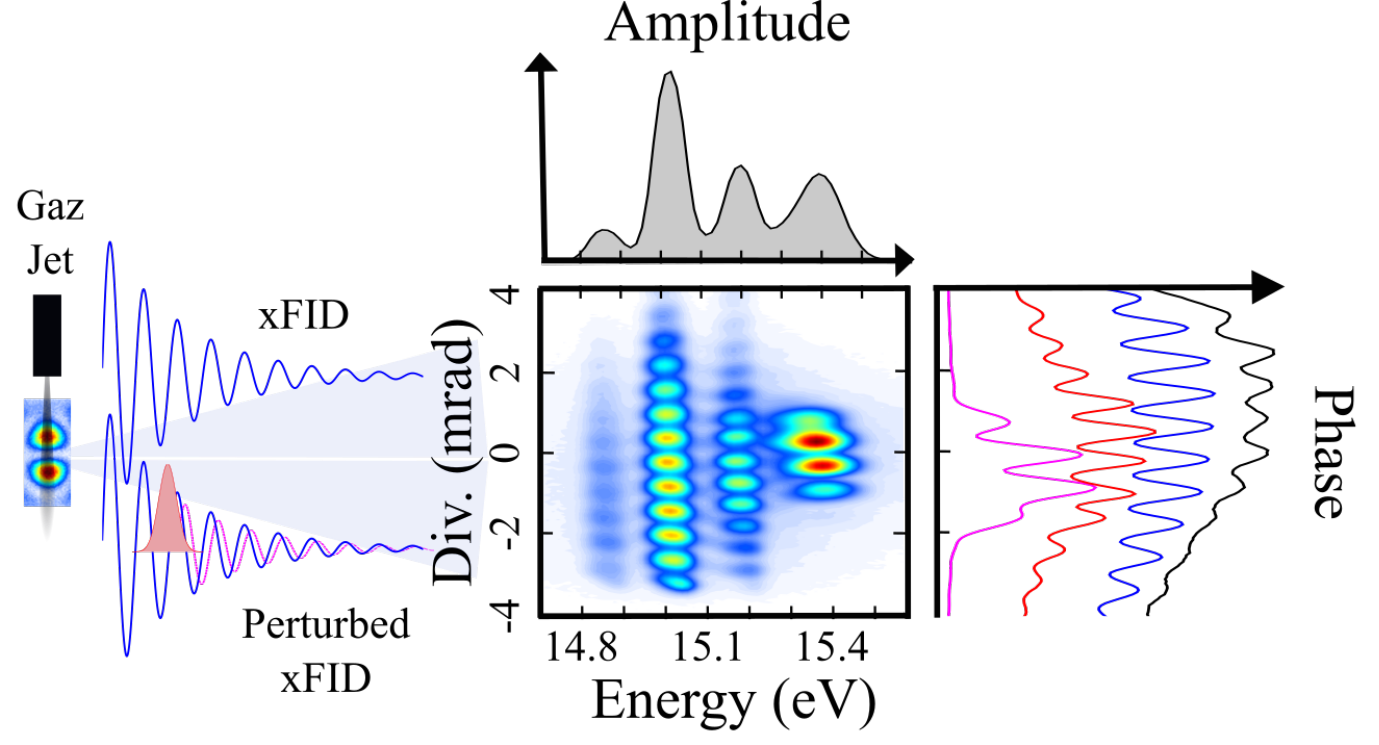
\includegraphics[width=.8\columnwidth]{Figures/Conclusion/xfid_deuxsources.png}%
\caption{Interférences observées en champ lointain entre deux sources de xFID séparées spatialement. Chacune des deux sources émet un rayonnement XUV à des énergies correspondant à 4 états de Rydberg de l'argon. Une impulsion infrarouge vient perturber et introduire un déphasage sur la source du bas, créant un décalage de ces franges. On mesure ainsi la phase relative des deux sources pour chacun des états.}
\label{fig:xfid_deuxsources}
\end{figure}

\subsection{Mesures de PECD résolue en temps}
Après avoir développé une source d'harmoniques polarisées elliptiquement, nous avons montré qu'elle pouvait être utilisée pour mesurer des dichroïsmes circulaires de photoélectron (PECD) dans des molécules chirales. Nous avons démontré cet effet dans la fenchone avant de comparer les résultats obtenus à des mesures réalisées sur la ligne DESIRS du synchrotron SOLEIL. En plus de présenter un accord satisfaisant, cette comparaison nous permet d'envisager une caractérisation complète de l'état de polarisation du rayonnement harmonique. Des mesures complémentaires doivent être réalisées pour conclure cette étude, comme détaillé en partie \ref{sec:soleil_vs_celia}. Une fois réalisées, nous envisageons d'utiliser le PECD pour caractériser le rayonnement produit par les différentes techniques de génération de polarisations elliptiques dans l'XUV, dans le but de choisir la plus adaptée à l'étude de dynamiques de molécules chirales.

\`A ce sujet, nous n'avons présenté ici que des mesures de PECD \textit{statiques}. Cette technique était jusque ici résolue en fréquence dans des expériences réalisées sur synchrotron. Nos travaux permettent de réaliser ces mêmes mesures sur une source ultra-brève et d'y ajouter une résolution temporelle. Nous avons commencé une série d'expériences pompe-sondes dans lesquelles on explore les dynamiques électroniques dans des potentiels chiraux. Dans un premier temps, nous nous sommes intéressés au cas plus simple à mettre en œuvre du PECD multi-photonique \mycite{LuxAC2012}. La première expérience réalisée, toujours au CELIA Bordeaux, utilise une impulsion de pompe polarisée linéairement à 200 pour exciter la molécule de fenchone vers les états de Rydberg 3s. L'impulsion de sonde, à 400 nm, est polarisée circulairement et ionise la molécule. Un PECD significatif est observé, signe que même pour un état de Rydberg éloigné du centre chiral, l'électron ionisé est toujours sensible au potentiel chiral. Ce PECD est ensuite étudié au cours du temps.

Un résultat étonnant est obtenu lorsque les impulsions de pompe et de sonde sont échangées. Dans ce cas, on observe toujours un PECD alors que l'impulsion de sonde est polarisée linéairement. L'asymétrie observée est surprenante car elle ne s'explique pas dans la description habituelle du PECD. En vérité, l'asymétrie est créée non pas durant l'ionisation, mais lors de l'excitation. L'impulsion de pompe, polarisée circulairement, crée une densité macroscopique chirale dans la molécule, révélée dans un second temps dans la distribution angulaire de photoélectron. 

Ces résultats, qui feront l'objet de prochaines publications, montrent une dynamique très riche due au potentiel moléculaire chiral. Ils constituent les premières mesures \textit{dynamiques} de PECD et plus généralement démontrent la possibilité d'effectuer des mesures chiroptiques ultra-rapides, très difficiles à réaliser par ailleurs. Dans la suite logique de cette démarche, nous prévoyons d'effectuer des expériences pompe-sondes XUV-Infrarouge, où on pourrait utiliser l'ionisation à deux photons pour observer des traces similaires au RABBIT (voir section \ref{sec:omabbit}). En plus de l'intensité des pics satellites habituels ($b_0$ dans le formalisme du PECD), on aura également accès à leur paramètre dichroïque, $b_1$. Comme on l'a vu, ce paramètre est très sensible aux finesses du potentiel chiral. Une analyse de type RABBIT pourrait donner accès aux délais de photoionisation entre les différents canaux d'ionisation et permettre d'observer des dynamiques moléculaires chirales, à l'échelle attoseconde. 

%% we want the numbering to start back at A
\renewcommand{\thesection}{\Roman{section}}
\setcounter{section}{0}
%it is going to mess hyperref links because it will have the same name as previous sections -> we change it
\renewcommand{\theHsection}{CL.\the\value{section}}
% same for figures
\renewcommand{\thefigure}{\Roman{section}.\arabic{figure}}
\setcounter{figure}{0}

\chapternonumtoc{Conclusions et Perspectives}
\makeatletter
\def\toclevel@chapter{-1}
\def\toclevel@section{0}
\def\toclevel@subsection{1}
\makeatother
%
%Nous avons étudié le comportement des deux types de moment angulaire dans la génération d'harmonique d'ordre élevé. Nous avons pu observer sa conservation, ce qui soutient la représentation de la GHOE comme un processus paramétrique. Cela permet également de transférer ces propriétés au rayonnement harmonique, c'est-à-dire à des impulsions ultra-brèves de très courte longueur d'onde. Dans ce chapitre de conclusion, nous récapitulons ces résultats et présentons les développements envisagés à partir de ces sources de lumière uniques. Nous discuterons successivement des deux composantes du moment angulaire de la lumière.
%
%\section{Perspectives d'utilisation de rayonnement XUV portant du MAO}
%Dans la partie \ref{CH:OAM_HHG}, nous avons d'abord discuté de la génération d'harmoniques d'ordre élevé à partir d'un faisceau de Laguerre-Gauss. Cette expérience s'ajoute à deux précédentes \mycite{ZurchNP2012,GariepyPRL2014} et étend l'étude du transfert de MAO à une gamme de paramètre bien plus large. Le moment angulaire orbital porté par le rayonnement harmonique a été caractérisé en utilisant les propriétés de divergences des faisceaux de Laguerre-Gauss, qui permettent d'obtenir la loi de transfert $\ell_q=q\times\ell_1$ attendue théoriquement \mycite{HernandezPRL2013}. Contrairement aux études précédentes, qui utilisent une méthode de caractérisation directe, notre raisonnement se base uniquement sur une observation du profil d'intensité harmonique en champ lointain. Il s'appuie sur des calculs analytiques et numériques (chapitre \ref{sec:OAM_analysis}) et sur le fait que dans un processus non-linéaire, les maxima du champ émis au foyer coïncident avec ceux du champ de génération, qui est lui bien caractérisé. Cette approche indirecte est applicable quelque soit la longueur d'onde générée, ce qui nous a permis d'étudier les cas où le laser de génération porte $\ell_1=1$, $2$ ou $3$ unités de MAO. La plus haute valeur de MAO harmonique est obtenue pour $\ell_1=3$, où $\ell_{19} = 57$. Nous avons également pu étendre l'étude à des longueurs d'ondes très courtes, jusqu'à $\lambda_{41} = 19.5$ nm, en utilisant le néon comme gaz de génération.
%
%\subsection{Génération de moment angulaire orbital arbitraire}
%Ces résultats nous amènent à envisager des applications utilisant ce rayonnement aux propriétés particulière. Notons pour commencer qu'il serait utile de disposer d'un rayonnement XUV portant de faibles valeurs de MAO. Le schéma direct présenté ici n'est pas très flexible puisque gouverné par la loi $\ell_q=q\times\ell_1$. Pour répondre à ce problème, nous avons implémenté un schéma à deux faisceaux non-colinéaires, initialement proposé par \mycite{GariepyPRL2014}. On y utilise un faisceau à 800 nm Gaussien qui croise un faisceau à 400 nm portant $\ell_1 = 1$ dans la zone d'interaction avec le jet de gaz. Ce dispositif est très similaire à celui présenté à la partie \ref{sec:calib} et se comprend dans une image photonique : l'harmonique d'ordre $q$ peut être générée par l'absorption de $q$ photons rouges, mais également de $q-4n$ photons rouges et $2n$ photons bleu. Le faisceau bleu étant non-colinéaire, la contribution du chemin $(q-4n,2n)$ sera décalée en champ lointain à mesure que $n$ augmente. De plus, le faisceau bleu portant $\ell_1=1$, la conservation du MAO impose que la contribution du chemin $(q-4n,2n)$ porte un MAO égal à $2n$. Ainsi, on peut générer à une longueur d'onde quelconque des faisceaux portant des valeurs très faibles de MAO.
%
%Cette expérience a été réalisé à l'université de Nova Gorica, en collaboration avec le groupe du Prof. G. De Ninno. Nous présentons des résultats préliminaires sur la figure \ref{fig:gauthier}, où on observe le spectre harmonique en champ lointain. 
%
%\begin{figure}[!ht]
%\centering
%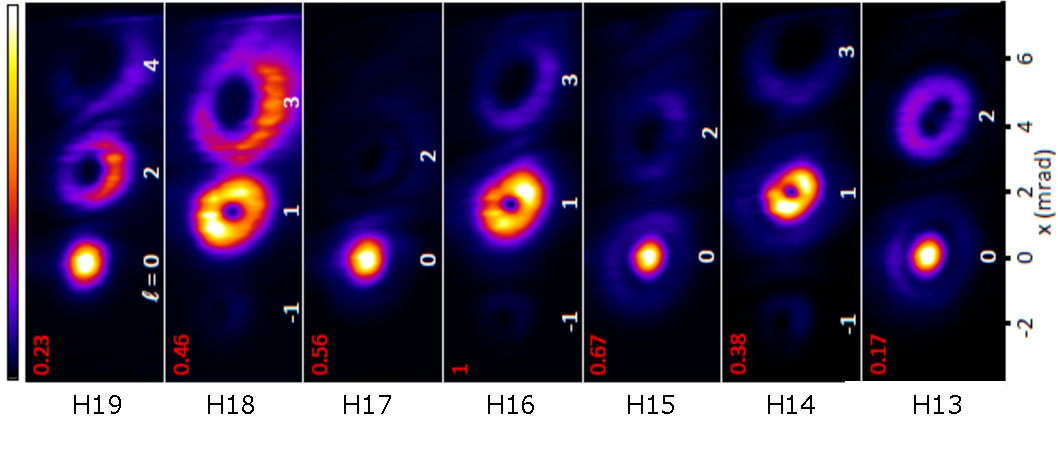
\includegraphics[width=0.8\columnwidth]{Figures/Conclusion/gauthier.pdf}%
%\caption{Intensité en champ lointain obtenue à partir du schéma à deux couleurs non-colinéaires. Chaque mode est repéré par le nombre de photons bleus absorbés, c'est-à-dire par leur moment angulaire orbital.}
%\label{fig:gauthier}
%\end{figure}
%Pour chaque harmonique, on observe de nombreux ordres de diffractions portant des valeurs de MAO différentes. Ces valeurs ont été confirmées par une mesure de front d'onde à l'aide d'un capteur de Hartmann, capable de résoudre la phase hélicoïdale pour ces faibles valeurs de $\ell$.
%
%\subsection{Impulsions ultra-courtes couplées spatio-temporellement}
%Dans un second temps, nous avons présenté une caractérisation complète du train d'impulsion attoseconde généré à partir d'un faisceau de Laguerre-Gauss. Pour ce faire, nous avons utilisé la technique RABBIT, qui permet de mesurer la phase relative entre chaque harmonique constituant le train d'impulsions. Ces mesures ont mis en évidence un problème intéressant : dans la technique RABBIT, le signal mesuré est intégré sur la totalité du volume d'interaction. Si on utilise une impulsion attoseconde portant du MAO et une impulsion d'habillage Gaussienne, la phase entre les deux faisceaux varie entre 0 et $2\pi$ dans le volume et la somme cohérente de ces contributions donne un résultat nul : les pics satellites de la trace RABBIT n'oscilleront pas. Nous avons donc utilisé une impulsion d'habillage portant le même MAO que celle de génération, de sorte à avoir un accord parfait entre les deux faisceaux au sein de la zone d'interaction. Il s'agit à notre connaissance de la première mesure de phase spectrale pour un faisceau non-Gaussien.
%
%\subsubsection{Mesures de phase spectrale résolues spatialement}
%Il est communément supposé que la phase spectrale varie peu selon les coordonnées spatiales, principalement car cette variation ne peut être résolue. En vérité, de nombreuses inhomogénéités peuvent introduire des couplages \textit{spatio-temporaux} dès l'impulsion laser de génération. On se reportera à la thèse de Gustave Pariente pour une discussion très complète sur la caractérisation de ces couplages dans le domaine infrarouge. Ils sont bien sûr transmis et amplifiés dans la GHOE, ce qui enlève une grande part de validité aux mesures intégrées spatialement. Un des axes principaux de recherche dans le domaine de la GHOE est la production d'impulsion attoseconde très énergétique, à partir de lasers de génération intenses qui interagissent sur plusieurs centimètres avec le milieu gazeux. Il est très probable que dans ces régimes extrêmes, les couplages spatio-temporaux dans l'XUV seront un facteur limitant à l'augmentation de l'intensité sur cible.
%
%Nos résultats suggèrent que la technique RABBIT habituelle pourrait être modifiée pour obtenir une partie de ces informations \textit{spectro-spatiales}. En effet, nous avons mis en évidence la possibilité de modifier le faisceau d'habillage pour avoir accord ou non avec le faisceau harmonique. Plutôt que d'accorder habillage et génération sur tout le volume, on pourrait restreindre de manière contrôlée la zone d'accord de sorte à mesurer la phase spectrale provenant seulement de cette partie du faisceau. Pour ce faire, il est plus simple d'utiliser l'intensité que la phase : si on utilise un faisceau d'habillage plus petit spatialement, seule la zone où les intensités des deux faisceaux sont non nulles contribuera à la trace RABBIT. 
%
%Nous avons réalisé des expériences préliminaires pour tester ce principe, dans le cadre d'une collaboration avec le groupe du Prof. L.F. DiMauro de la Ohio State University (Columbus OH, USA). Comme cas test, on cherche à caractériser un mode de Laguerre-Gauss XUV, pour lequel la phase varie linéairement avec la coordonnée azimutale. Pour le faisceau d'habillage, nous avons utilisé une lame de phase présentant une marche de $\pi$ \mycite{CamperPRA2014}. Cette lame crée au foyer deux tâches focales séparées de $\sim \SI{100}{\micro\metre}$, comme représenté sur la figure \ref{fig:spatialrabbit}. 
%
%\begin{figure}[!ht]
%\centering
%\def\svgwidth{\columnwidth}
%\import{Figures/Conclusion/}{spatial_rabbit.pdf_tex}
%\caption{Principe d'une expérience RABBIT résolue spatialement. Le faisceau de génération (a) donne un profil de LG aux harmoniques générées. Le faisceau d'habillage (b) présente deux tâches focales, séparées d'une distance similaire au diamètre de l'anneau de génération. Ce profil peut être tourné d'un angle noté $\theta$. (c) La contribution à la mesure RABBIT est déterminée par le recouvrement entre ces deux profils d'intensité. (d) Pour chaque valeur de $\theta$, on mesure les oscillations des pics satellites dans la trace RABBIT. La phase de ces pics satellites nous donne $\phi_q(\theta)$.}
%\label{fig:spatialrabbit}
%\end{figure}
%
%Si le faisceau d'habillage (\ref{fig:spatialrabbit}.b) est ajusté pour avoir une taille similaire à l'anneau du faisceau de génération (\ref{fig:spatialrabbit}.a), on peut limiter la zone contribuant à la mesure RABBIT (\ref{fig:spatialrabbit}.c). La lame de phase $0-\pi$ est montée sur une rotation motorisée, permettant de sélectionner l'angle contribuant à la trace RABBIT. Pour chaque valeur de cette angle $\theta$, on mesure les oscillations à 2$\omega$ des pics satellites. La phase de ces oscillations donne donc la phase spectrale résolue angulairement, $\phi_q(\theta)$. La figure (\ref{fig:spatialrabbit}.d) illustre le décalage entre $\theta_1$ et $\theta_1+\pi/2$ pour une phase spectrale quelconque. Pour un faisceau de Laguerre-Gauss idéal de moment $\ell_q$, on s'attend à mesurer $\phi_q(\theta) = \ell_q\theta+2\Delta t_e\omega_q$, où $\Delta t_e$ est le temps d'émission de l'atome de détection utilisé. Ces expériences n'ont pour l'instant pas été conclues, mais ce principe pourrait être généralisé à des mesures spatiales selon d'autres coordonnées.
%
%\subsubsection{Utilisation du couplage spatio-temporel en physique ultra-rapide}
%Les mesures RABBIT réalisées nous ont permis de reconstruire complètement le profil spatio-temporel du train attoseconde généré. Dans le cas de faisceaux portant du MAO, on obtient un profil d'intensité très particulier à deux spirales imbriquées. Cela met en évidence un couplage spatio-temporel très fort, où l'intensité est retardée temporellement avec la coordonnée azimutale. Nous discutons ici des possibilités d'utiliser les couplages spatio-temporels des faisceaux de LG en physique ultra-rapide.
%
%Comme on l'a mentionné, les couplages spatio-temporels sont souvent non désirables en physique des champs forts. Toutefois, \mycite{VincentiPRL2012} ont montré qu'ils pouvaient aussi être introduits volontairement pour contrôler l'émission harmonique. Dans leur schéma, on utilise un prisme cale (\textit{wedge} en anglais) pour introduire une rotation de front d'onde au foyer au cours du temps, qui émet chaque impulsion attoseconde selon une direction angulaire donnée. \linebreak
%Un faisceau de Laguerre-Gauss, de par sa phase $\ell\theta$, présente également un couplage spatio-temporel. La phase en un point donné évolue entre 0 et $\ell 2\pi$ pendant un cycle optique, on peut donc l'utiliser pour observer des phénomènes sub-cycles. Nous illustrons cette possibilité en commençant par un faisceau de Laguerre-Gauss infrarouge.
%
%Intéressons-nous à la génération d'harmonique à deux couleurs. Dans ce schéma, des harmoniques sont générées par un faisceau à 800 nm superposé à sa deuxième harmonique, à 400 nm. Cette seconde couleur brise la centro-symétrie de la GHOE, qui était responsable de la génération d'harmoniques impaires uniquement. On obtient donc un spectre composé des harmoniques paires et impaires du laser de génération. \mycite{DudovichNP2006} ont montré que quand le champ à 400 nm est très faible, il vient simplement perturber le phénomène de GHOE habituel : au cours de l'étape de propagation du modèle à trois étapes, la trajectoire électronique est légèrement modifiée. Une analyse perturbative montre qu'en changeant le délai entre les deux couleurs, il est possible de remonter au temps d'émission électronique, ainsi qu'aux paramètres $t_i$ et $\bm{p}$ du modèle SFA \mycite{PedatzurNP2015}. L'observable mesurée ici est l'intensité harmonique en fonction du délai rouge-bleu noté $\tau$. Elle s'écrit dans le cas perturbatif et si les polarisations des champs sont parallèles :
%\begin{equation}
%I_q(\tau)=
%\begin{cases}
%I_1 + I^q_0\left|\cos(\omega_{800}\tau+\phi_q)\right|^2\text{ si $q$ impair}\\
%I_2 + I^q_0\left|\sin(\omega_{800}\tau+\phi_q)\right|^2\text{ si $q$ pair}
%\end{cases}
%\label{eq:oren}
%\end{equation}
%L'information à extraire est $\phi_q$, on peut donc effectuer un scan de délai entre les deux faisceaux (figure \ref{fig:rb_mapping}.a). Une autre approche est de paramétrer ce délai spatialement de sorte à ne pas avoir à faire de scan. Prenons par exemple des faisceaux rouges et bleus portant chacun $\ell=1$. Leur phase s'écrit au point $(r,\theta)$ :
%\begin{align}
%\varphi_{400}(r,\theta,t) &= \omega_{400}(t + \theta/\omega_{400}),\\
%\varphi_{800}(r,\theta,t) &= \omega_{800}(t + \theta/\omega_{800}).
%\end{align}
%Le délai les séparant s'écrit donc en tout point $\tau(r,\theta) = \theta/\omega_{800}-\theta/\omega_{400} = \theta/\omega_{400}$, ce qui est tracé en \ref{fig:rb_mapping}.b. On a donc un délai variant spatialement : le délai rouge-bleu est paramétré sur la coordonnée azimutale. On retrouvera donc l'évolution temporelle de l'intensité des harmoniques sur leur coordonnée azimutale, comme illustré sur la figure \ref{fig:rb_mapping}.c.
%\begin{figure}[!ht]
%\centering
%\def\svgwidth{\columnwidth}
%\import{Figures/Conclusion/}{rb_lg_mapping.pdf_tex}
%\caption{Principe d'expériences de GHOE à deux couleurs utilisant le couplage spatio-temporel des faisceaux de LG. L'expérience habituelle est de mesurer le spectre harmonique en fonction du délai rouge-bleu (a). Si on utilise des faisceaux de LG, on a un délai variant azimutalement (b). Les harmoniques générées sont donc modulées selon $\theta$, ce qui permet de mesurer $\phi_q$ sans effectuer de scan (lignes pointillées rouges).}
%\label{fig:rb_mapping}
%\end{figure}
%Expérimentalement, les harmoniques sont observées en champ lointain. Nous ne pouvons pas réaliser le calcul de propagation car nous ne connaissons pas la phase spatiale des harmoniques, elle aussi perturbée par le champ à 400 nm. Nous prévoyons d'effectuer des calculs SFA 4D complets pour prédire et quantifier cet effet. Dans tous les cas, l'observable $\phi_q$ se retrouvera dans le profil spatial en champ lointain. On peut donc mesurer la quantité recherchée en un seul tir laser, plutôt qu'en effectuant un scan de délai.
%
%Dans le cas de faisceaux de Laguerre-Gauss dans l'XUV, on a la même propriété de phase paramétrée avec l'angle. De plus, si on considère non plus une harmonique donnée mais l'impulsion attoseconde entière, l'intensité a un profil de \textit{light spring}. Chaque point de l'espace $(r,\theta)$ voit donc un train d'impulsion attoseconde qui se décale temporellement de façon linéaire avec $\theta$. Cette propriété pourrait être utilisée dans une expérience d'absorption transitoire, dans laquelle on mesure habituellement l'intensité transmise par un échantillon, intégrée spatialement, au cours du temps. Avec un light spring, on pourrait plutôt résoudre spatialement l'intensité transmise, dans laquelle chaque valeur de $\theta$ correspond à une valeur de délai différente.
%
%\subsection{Spectroscopies utilisant le moment angulaire orbital XUV}
%En plus de ces couplage spatio-temporels, les faisceaux de Laguerre-Gauss possèdent un intérêt plus fondamental : les photons y portent un moment angulaire orbital bien défini. Il est très tentant de voir cette grandeur comme un paramètre supplémentaire pour contrôler et étudier l'interaction laser-matière. Par exemple, la perspective de nouvelles règles de sélection en photoionisation permettrait d'étudier des niveaux atomiques normalement interdits. Dans la partie \ref{sec:selectionrules}, nous avons montré que la réalité n'était pas si clémente : le MAO se couple préférentiellement au moment externe d'un atome. Le couplage avec le moment interne de l'atome n'apparaît qu'au second ordre. C'est également ce qui est observé dans nos mesures RABBIT : si la photoionisation était modifiée par la présence de MAO, on aurait mesuré un temps d'émission différent de celui obtenu en faisceau gaussien\footnote{En effet, le temps d'émission dépend du niveau électronique ionisé. Par exemple, \mycite{SchultzeScience2010} ont mesuré un délai de 21 as entre les électrons issus de l'orbitale 2p du néon par rapport à ceux issus de la 2s.}.
%
%Dans notre expérience, nous disposions d'un faisceau de diamètre $\sim \SI{100}{\micro\metre}$ au foyer, à comparer avec un atome d'argon dont le diamètre est de l'ordre de l'Angström. Là est le problème principal : à l'échelle de l'atome, la phase du faisceau de LG est plate. Il n'y a qu'au centre du faisceau que la phase varie à l'échelle de l'atome, mais l'intensité y est nulle. Une transition quadripolaire dépendant du gradient du champ électrique, il est naturel qu'on ne les observe pas  dans notre cas. Pour cette raison, l'intégralité des prédictions théoriques se sont jusqu'à présent limitées à des valeur d'intensité et de focalisation non réalisables en pratique. Par exemple, \mycite{PiconOE2010} prédisent une modification des règles de sélection pour l'atome d'hydrogène, avec un faisceau à 27.2 eV, de waist $\SI{4.79}{\micro\metre}$ et d'intensité égale à $\SI{6.8e18}{\W\per\centi\metre\squared}$. De même, \mycite{WatzelPRA2016} proposent une mesure de délais attosecondes de sous-niveaux magnétiques de l'argon à partir d'un faisceau à 90 eV et d'intensité $\SI{5.6e19}{\W\per\centi\metre\squared}$.
%
%De telles intensités dans l'XUV dépassent l'état de l'art actuel de nombreux ordres de grandeurs. S'il est certain que les intensités XUV disponibles continueront d'augmenter dans le futur, il est sûrement plus simple de chercher des systèmes plus adaptés, c'est-à-dire plus gros par rapport au faisceau harmonique. Par exemple, un atome de Rydberg a un rayon déjà bien plus important : pour le niveau n=137 de l'hydrogène, il vaut $\sim\SI{1}{\micro\metre}$. D'autres candidats sont les agrégats d'atome, ou bien des molécules de $\text{C}_{60}$, un des plus gros objets dans lequel a été observée la dualité onde-particule \mycite{ArndtNat1999}. Leur interaction avec un faisceau portant du MAO est étudié théoriquement par \mycite{WatzelPRA2016}, qui observent un effet pour une intensité de $\SI{3.2e17}{\W\per\centi\metre\squared}$ à 90 eV. L'intensité est réduite par rapport à l'argon mais pas de manière suffisante pour envisager une expérience.\linebreak
%Peut-être que les cibles adaptées aux capacités expérimentales actuelles ne doivent pas être cherchées parmi les molécules, mais plutôt dans la phase condensée. Il est en effet possible de créer optiquement des excitations collectives à la surface ou dans le volume d'un solide, dont certaines pourraient être sensibles au MAO. Deux propositions intéressantes existent en ce sens : \mycite{VanVeenendaalPRL2007} prédit un dichroïsme induit par le MAO dans l'absorption au point K de métaux de transitions, tandis que \mycite{VanVeenendaalPRB2015} discute de l'interaction entre un faisceau de LG XUV et un vortex magnétique. Nous sommes en train d'évaluer la faisabilité expérimentale de ces propositions.
%
%En conclusion, il nous semble très intéressant de continuer à développer le contrôle de faisceaux harmoniques portant du moment angulaire orbital. Les utilisations les plus immédiates nous paraissent être celles utilisant les propriétés macroscopiques de ces faisceaux. Nous avons mentionné l'utilisation de la structure spatio-temporelle des modes de LG et des impulsions attosecondes générées. Notons au passage que cette structure survit dans le cas d'impulsions attosecondes isolées \mycite{HernandezPRL2013}. Il serait également assez direct d'utiliser les faisceaux de LG XUV en imagerie. En effet, ils sont déjà utilisés dans le domaine visible pour la microscopie \mycite{FurhapterOL2005} et commencent à être étudiés pour l'imagerie par diffraction cohérente \mycite{wangOE2009}. La résolution de ces deux techniques est grandement améliorée par l'utilisation de rayonnement XUV; nos résultats permettent donc d'envisager la combinaison avantageuse de faibles longueurs d'ondes et de modes de LG. \linebreak
%Quant aux applications de rayonnement XUV portant du MAO en spectroscopie, il est probablement trop tôt pour prédire la marche à suivre. L'étude théorique de l'interaction doit continuer à se développer en se dirigeant vers des conditions plus réalistes expérimentalement, tandis que la production expérimentale de faisceaux intenses et fortement focalisés doit être optimisée dans l'XUV. La focalisation dans ces gammes spectrales est particulièrement étudiée par la communauté des lasers à électron libre, où des tâches focales de l'ordre de 10 nm ont été obtenues \mycite{ChaoNature2005}. Ces grands instruments ouvrent d'ailleurs une autre voie de recherche, illustrée par de récentes propositions \mycite{RibiPRL2014,HemsingPRL2011,HemsingPRL2012}. Elles visent à contrôler le moment angulaire orbital de lasers à électron libre, qui fournissent un rayonnement XUV très intense. Nous avons eu la chance de participer aux premiers essais d'implémentation sur FERMI (Trieste, Italie) et tenons à remercier Prof. G. De Ninno et D. Gauthier pour cette opportunité.
%
%\section{Conclusions et perspectives sur le moment angulaire de spin}
%Dans la partie \ref{PA:Spin_HHG}, nous avons étudié l'effet du moment angulaire de spin dans la génération d'harmoniques d'ordre élevé. Nous avons vu qu'il y est conservé, mais que l'efficacité du processus habituel chute fortement à mesure que l'ellipticité du laser de génération augmente. Nous avons étudié la GHOE au voisinage d'une résonance du milieu de génération, dans le cas d'une résonance près du seuil de l'argon, et d'une résonance de forme dans le continuum d'une molécule, ici \sf6. Aux énergies résonantes, on observe une forte augmentation de l'ellipticité harmonique attribuée à une modification de la dynamique électronique au moment de la recombinaison. Cette interprétation est soutenue par des calculs TDSE, réalisés par B. Pons et B. Fabre. 
%
%\subsection{GHOE proche du seuil de l'argon : l'effet xFID}
%Dans le cas particulier de l'argon, ces expériences ont mis en évidence le phénomène de xFID. Il a été étudié en détail par \mycite{beaulieuArXiv2016}. En collaboration avec Samuel Beaulieu, \'{E}tienne Bloch, Valérie Blanchet et Yann Mairesse, nous avons poursuivi ces expériences en utilisant une longueur d'onde de 400 nm et en choisissant des conditions de focalisation favorisant grandement le xFID. Dans ce processus, on crée une superposition cohérente entre l'état fondamental et plusieurs états de Rydberg de l'atome. Le paquet d'onde ainsi créé se désexcite en émettant un rayonnement XUV cohérent. Cet effet n'est pas très différent de celui utilisé en absorption transitoire attoseconde (ATAS, pour \textit{Attosecond Transient Absorption Spectroscopy}) \mycite{BeckNJP2014}, dans laquelle les oscillations d'un dipôle induit par une excitation XUV sont observées à l'aide d'une seconde impulsion infrarouge. Il est possible de réaliser une expérience pompe-sonde similaire en perturbant l'émission xFID à l'aide d'une impulsion infrarouge de délai variable. Des expériences préliminaires démontrent la possibilité de résoudre les battements femtoseconde du paquet d'onde électronique créé dans l'argon. \`A ces mesures d'amplitude nous prévoyons d'ajouter une mesure de phase en utilisant la technique d'interférométrie à deux sources développée par \mycite{CamperThesis2014}. Dans cette technique, on crée deux sources de xFID séparées spatialement qui interfèrent en champ lointain. En perturbant une seule des deux sources avec une impulsion infrarouge, on retrouve le déphasage induit dans ces interférences spatiales. La figure \ref{fig:xfid_deuxsources} présente un exemple de franges observées à l'aide de ce dispositif. Ces expériences sont toujours en cours au CELIA Bordeaux. 
%
%\begin{figure}[!ht]
%\centering
%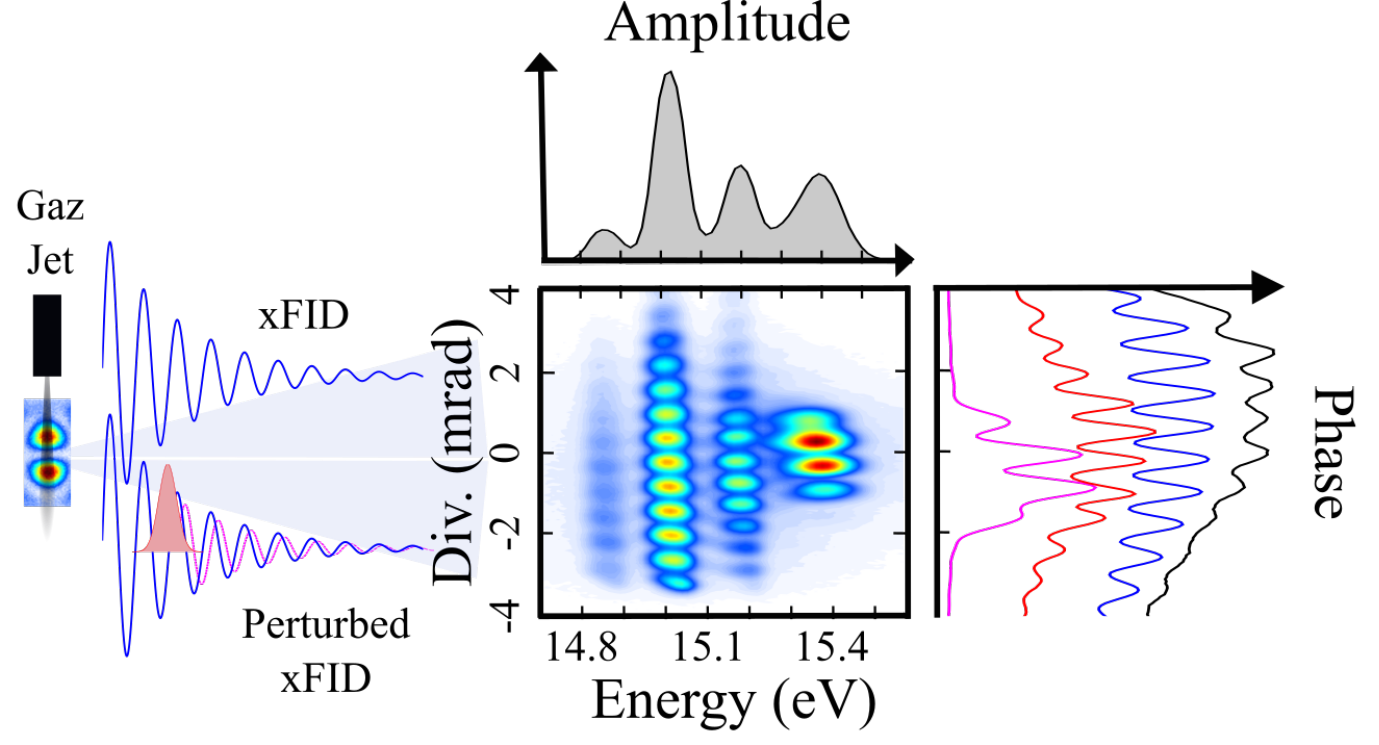
\includegraphics[width=.8\columnwidth]{Figures/Conclusion/xfid_deuxsources.png}%
%\caption{Interférences observées en champ lointain entre deux sources de xFID séparées spatialement. Chacune des deux sources émet un rayonnement XUV à 4 énergies différentes qui correspondent aux états de Rydberg de l'argon. Une impulsion infrarouge vient perturber et introduire un déphasage sur la source du bas, créant un décalage de ces franges. On mesure ainsi la phase relative des deux sources pour chacun des états.}
%\label{fig:xfid_deuxsources}
%\end{figure}
%
%\subsection{Mesures de PECD résolue en temps}
%Après avoir développé une source d'harmoniques polarisées elliptiquement, nous avons montré qu'elle pouvait être utilisée pour mesurer des dichroïsmes circulaires de photoélectron (PECD) dans des molécules chirales. Nous avons démontré cet effet dans la fenchone avant de comparer les résultats obtenus à des mesures réalisées sur la ligne DESIRS du synchrotron SOLEIL. En plus de présenter un accord satisfaisant, cette comparaison nous permet d'envisager une caractérisation complète de l'état de polarisation du rayonnement harmonique. Des mesures complémentaires doivent être réalisées pour conclure cette étude, comme détaillé en partie \ref{sec:soleil_vs_celia}. Une fois réalisées, nous envisageons d'utiliser le PECD pour caractériser le rayonnement produit par les différentes techniques de génération de polarisations elliptiques dans l'XUV, dans le but de choisir la plus adaptée à l'étude de dynamiques de molécules chirales.
%
%Dans ce manuscrit, nous n'avons présenté que des mesures de PECD \textit{statiques}. Nous reproduisons donc les mesures synchrotron, bien résolues en fréquence. En plus de les reproduire, nos travaux permettent de réaliser ces mesures sur une source ultra-brève et d'y ajouter une résolution temporelle. Nous avons commencé une série d'expériences pompe-sondes dans lesquelles on explore les dynamiques électroniques dans des potentiels chiraux. Dans un premier temps, nous nous sommes intéressés au cas plus simple à mettre en œuvre du PECD multi-photonique \mycite{LuxAC2012}. La première expérience réalisée, toujours au CELIA Bordeaux, utilise une impulsion de pompe polarisée linéairement à 200 nm pour exciter la molécule de fenchone vers les états de Rydberg 3s. L'impulsion de sonde, à 400 nm, est polarisée circulairement et ionise la molécule. Un PECD significatif est observé, signe que même pour un état de Rydberg éloigné du centre chiral, l'électron ionisé est toujours sensible au potentiel chiral. Ce PECD est ensuite étudié au cours du temps.
%
%Un résultat étonnant est obtenu lorsque les impulsions de pompe et de sonde sont échangées. Dans ce cas, on observe toujours un PECD alors que l'impulsion de sonde est polarisée linéairement. L'asymétrie observée est surprenante car elle ne s'explique pas dans la description habituelle du PECD. En vérité, l'asymétrie est créée non pas durant l'ionisation, mais lors de l'excitation. L'impulsion de pompe, polarisée circulairement, crée une densité macroscopique chirale dans la molécule, révélée dans un second temps dans la distribution angulaire de photoélectron. 
%
%Ces résultats, qui feront l'objet de prochaines publications, montrent une dynamique très riche due au potentiel moléculaire chiral. Ils constituent les premières mesures \textit{dynamiques} de PECD et plus généralement démontrent la possibilité d'effectuer des mesures chiroptiques ultra-rapides, extrêmement difficiles à réaliser par ailleurs. Dans la suite logique de cette démarche, nous prévoyons d'effectuer des expériences pompe-sondes XUV-Infrarouge, où on pourrait utiliser l'ionisation à deux photons pour observer des traces similaires au RABBIT (voir section \ref{sec:omabbit}). En plus de l'intensité des pics satellites habituels ($b_0$ dans le formalisme du PECD), on aura également accès à leur paramètre dichroïque, $b_1$. Comme on l'a vu, ce paramètre est très sensible aux finesses du potentiel chiral. Une analyse de type RABBIT pourrait donner accès aux délais de photoionisation entre les différents canaux d'ionisation et permettre d'observer des dynamiques moléculaires chirales, à l'échelle attoseconde. 
%
%\section{Le couplage spin-orbite optique}
%Notons pour conclure qu'au cours de cette thèse, nous nous sommes efforcés de séparer moment angulaire de spin et orbital. La séparabilité de ces deux quantités est un sujet d'étude à part entière, mais en général leur effet respectif dans une interaction laser-matière est identifiable. L'exemple le plus visuel est le mouvement d'une particule, mise en rotation sur elle-même par le MAS et autour du centre du faisceau par le MAO. Toutefois, en 2002 apparaît la première observation d'un couplage spin-orbite optique \mycite{BomzonAPL2001}. Dans certains processus, on peut avoir conservation du moment angulaire total mais une variation du MAS et du MAO. S'ensuivent plusieurs études de milieux exotiques où on a conversion entre MAS et MAO, tels que les cristaux uniaxiaux \mycite{BrasseletOL2009}, des milieux présentant un gradient de constante diélectrique, qui montrent des "effets Hall de spin" \mycite{OnodaPRL2004} et des "effets Hall de MAO" \mycite{BliokhPRL2006}, ou encore dans des "q-plates" \mycite{MarrucciPRL2006}. On a également un effet de conversion dans des faisceaux très fortement focalisés \mycite{ZhaoPRL2007}. S'il est difficile d'affirmer aujourd'hui quand et comment un couplage spin-orbite optique sera observé dans l'XUV, nos travaux nous autorisent au moins à envisager cette question. 
%


%
%%Nous disposons désormais d'une source de lumière unique : nous pouvons générer un rayonnement dans l'XUV portant du moment angulaire orbital, et temporellement extrêmement bref. Pour améliorer encore la flexibilité de la source, il serait intéressant de dévier de la loi $\ell_q=q\times\ell_1$ et de pouvoir accorder le MAO de chaque harmonique. Des expériences à cet effet sont en cours à Saclay et en collaboration avec le groupe du professeur G. De Ninno à l'université de Nova Gorica (Slovénie). Enfin, nous avons également participé aux premières expériences visant à transférer du MAO dans un laser à électron libre selon le principe proposé par \mycite{RibiPRL2014}. Les premiers essais ont été réalisés sur le laser à électron libre Fermi à Trieste (Italie). 
%%
%%Ces développements nous amènent à réfléchir aux applications à donner à ces sources de lumière uniques. D'un point de vue fondamental, il serait très intéressant d'observer un effet du MAO dans la photoionisation, c'est-à-dire d'identifier des contributions quadripolaires où plus d'une unité de $\ell$ est échangée. Comme on l'a observé dans l'expérience de RABBIT, un atome est un système bien trop petit par rapport à $\lambda$ pour espérer voir un tel effet. Au contraire, il est probable que des systèmes plus gros tels que de grosses molécules ou des solides soient plus intéressants. Parmi les rares études théoriques du sujet disponible, on trouve quand même quelques prédictions d'effets remarquables, comme le \textit{dichroïsme hélicoïdal} \mycite{VanVeenendaalPRL2007}.
%%D'un point de vue plus pratique, la structure d'intensité et de phase d'un champ de Laguerre-Gauss peut être directement utilisée. Par exemple, les développements de microscopie par faisceau de LG dans le domaine visible \mycite{FurhapterOL2005} pourraient être avantageusement transféré dans le domaine XUV. La diffraction cohérente, une autre technique d'imagerie, peut également bénéficier de l'utilisation de modes de LG \mycite{wangOE2009}. Enfin, les couplages spatio-temporels mis en évidence plus haut peuvent être mis à profit dans de nombreuses expériences résolues en temps, en utilisant le correspondance angle/retard de ces faisceaux. \mycite{ParienteOL2015} présente également des applications en accélération laser-plasma.


%Appendices
\appendix
\addcontentsline{toc}{part}{Annexes}
\renewcommand{\theHsection}{AN.\the\value{section}}
\makeatletter
\def\toclevel@chapter{0}
\def\toclevel@section{1}
\def\toclevel@subsection{2}
\makeatother

\chapter{Démonstrations de la partie I}
\section{Invariance de l'équation de Lagrange par changement de coordonnées}
Nous démontrons ici l'équation \ref{eq:lagq}. L'espace des configurations est décrit par ${q_j}$, $j\in[1,\;3N]$, qui s'écrivent en fonction des coordonnées cartésiennes ${x_i}$ et du temps :
\begin{equation}
\begin{split}
\forall j, q_j=q_j(x_1,\ldots,x_N,t)\text{ et inversement, }
\end{split}
\begin{split}
\forall i, x_i=x_i(q_1,\ldots,q_N,t).
\end{split}
\end{equation}

L'équation de Lagrange s'écrit :
\begin{equation}
\label{eq:lagapp}
\frac{d}{dt}\frac{\partial L}{\partial \dot{x}_i}-\frac{\partial L}{\partial x_i}=0,
\end{equation}

Réécrivons \ref{eq:lagapp} en fonction des ${q_j}$. On a : 
\begin{equation}
\label{eq:lag1}
\frac{\partial L}{\partial \dot{x}_i} = \sum_j \frac{\partial L}{\partial q_j} \frac{\partial q_j}{\partial \dot{x}_i}+ \sum_j\frac{\partial L}{\partial \dot{q}_j}\frac{\partial \dot{q}_j}{\partial \dot{x}_i}.
\end{equation}
$q_j$ ne dépend que de $x_i$ et $t$, donc ${\partial q_j}/{\partial \dot{x}_i}=0$ et le premier terme s'annule. De plus,
\begin{equation}
\dot{q}_j = \sum_i \frac{\partial q_j}{\partial x_i}\dot{x}_i+\frac{\partial q_j}{\partial t}\text{,  donc  }
\frac{\partial \dot{q}_j}{\partial \dot{x}_i}=\frac{\partial q_j}{\partial x_i}.
\label{eq:lag3}
\end{equation}
\ref{eq:lag1} donne donc :
\begin{equation}
\label{eq:lag2}
\frac{\partial L}{\partial \dot{x}_i} = \sum_j\frac{\partial L}{\partial \dot{q}_j}\frac{\partial q_j}{\partial x_i}.
\end{equation}
L'équation de Lagrange en coordonnées cartésiennes comprend la dérivée temporelle de cette expression, qui s'écrit :
\begin{align}
\frac{d}{dt}\frac{\partial L}{\partial \dot{x}_i} &= 
\sum_j\left(\frac{d}{dt}\frac{\partial L}{\partial \dot{q}_j}\right)\frac{\partial q_j}{\partial x_i}+
\sum_j\frac{\partial L}{\partial \dot{q}_j}\left(\frac{d}{dt}\frac{\partial q_j}{\partial x_i}\right) \\
&=\sum_j \left(\frac{d}{dt}\frac{\partial L}{\partial \dot{q}_j}\right)\frac{\partial q_j}{\partial x_i}+\sum_j\frac{\partial L}{\partial \dot{q}_j}\left(\sum_k \frac{\partial^2q_j}{\partial x_i \partial x_k}\dot{x}_k + \frac{\partial^2q_j}{\partial x_i \partial t}\right).
\end{align}
Par ailleurs, le second terme de l'équation de Lagrange s'écrit :
\begin{align}
\frac{\partial L}{\partial x_i}&= \sum_j \frac{\partial L}{\partial q_j} \frac{\partial q_j}{\partial x_i}+ \sum_j\frac{\partial L}{\partial \dot{q}_j}\frac{\partial \dot{q}_j}{\partial x_i} \\
&=\sum_j \frac{\partial L}{\partial q_j} \frac{\partial q_j}{\partial x_i}+ \sum_j\frac{\partial L}{\partial \dot{q}_j}\left(\sum_k \frac{\partial^2q_j}{\partial x_i \partial x_k}\dot{x}_k + \frac{\partial^2q_j}{\partial x_i \partial t}\right),
\end{align}
où on a utilisé \ref{eq:lag3}. On connaît maintenant tous les termes de l'équation de Lagrange en fonction des ${q_j}$, et en les soustrayant un terme s'annule, ce qui donne :
\begin{equation}
\sum_j\left(\frac{d}{dt}\frac{\partial L}{\partial \dot{q}_j}-\frac{\partial L}{\partial q_j}\right)\frac{\partial q_j}{\partial x_i}=0.
\end{equation}
$\frac{\partial q_j}{\partial x_i}$ est non singulière puisque son inverse est $\frac{\partial x_i}{\partial q_j}$, une quantité finie. Comme les $q_j$ sont tous indépendants, on obtient l'équation de Lagrange en coordonnées généralisées : 
\begin{equation}
\label{eq:lagqapp}
\frac{d}{dt}\frac{\partial L}{\partial \dot{q}_i}-\frac{\partial L}{\partial q_i}=0.
\end{equation}
Nous avons donc démontré que l'équation de Lagrange est invariante par changement des coordonnées utilisées pour décrire le système, ce qui en fait une formulation très pratique. 

\section{Composantes longitudinale et transverse du moment angulaire classique}
\label{app:calculj}
On démontre ici les relation \ref{eq:Jlong4} puis \ref{eq:Jtran}, expressions des composantes longitudinales et transverse de $\bm{J}$ en électromagnétisme classique.

\subsubsection{Composante longitudinale}
On considère le système {lumière+particules}. La contribution de $E_{\parallel}$ au moment angulaire du système s'écrit : 
\begin{align}
\bm{J}_{\parallel}&=\int{\epsilon_0\bm{r}\times(\bm{E}_{\parallel}\times\bm{B})\rmd\bm{r}}\nonumber\\
&=\epsilon_0\int{\bm{r}\times(\bm{E}_{\parallel}\times\left[\bm{\nabla}\times\bm{A}_{\bot}\right])\rmd\bm{r}}\text{, où on a utilisé \ref{eq:para15}}%&=\epsilon_0\int{\left(\sum_{a=x,y,z} E^a_{\parallel}(\bm{r}\times\bm{\nabla})A^a_{\bot}-\bm{r}\times(\bm{E}_{\parallel}\cdot\bm{\nabla})\bm{A}_{\bot}\right)\rmd\bm{r}}.
\label{eq:Jlong1app}
\end{align}

\'Ecrivons la $n$-ième composante de $\bm{r}\times(\bm{E}_{\parallel}\times\left[\bm{\nabla}\times\bm{A}_{\bot}\right])$. On utilise la convention d'écriture où une somme sur les indices indice répétés est implicite. Tout d'abord,
\begin{align}
\left(\bm{E}_{\parallel}\times\left[\bm{\nabla}\times\bm{A}_{\bot}\right]\right)_n &= 
(E_i\nabla_nA_i-E_i\nabla_iA_n)
\end{align}
On utilise ensuite le symbole de Levi-Civita $\epsilon_{lmn}$, défini par 
\begin{equation}
\epsilon_{lmn}=\left\lbrace
\begin{array}{rl}
0,& \mbox{si un des trois indices apparaît plus d'une fois}\\
1,&\mbox{si }l,m,n\mbox{ est une permutation paire de 1,2,3}\\
-1,&\mbox{si }l,m,n\mbox{ est une permutation impaire de 1,2,3}\\
\end{array}
\right.
\end{equation}
On écrit le produit vectoriel comme :
\begin{align}
r\times\left(\bm{E}_{\parallel}\times\left[\bm{\nabla}\times\bm{A}_{\bot}\right]\right)_l &= 
\epsilon_{lmn}r_m(E_i\nabla_nA_i-E_i\nabla_iA_n)\\
&=\epsilon_{lmn}r_mE_i\nabla_nA_i-\epsilon_{lmn}E_i\nabla_i(r_mA_n)+\epsilon_{lmn}E_i\nabla_i(r_m)A_n.
\end{align}
On a $\nabla_i(r_m)=\delta_{im}$, donc
\begin{align}
r\times\left(\bm{E}_{\parallel}\times\left[\bm{\nabla}\times\bm{A}_{\bot}\right]\right)_l 
&=E_i\epsilon_{lmn}r_m\nabla_nA_i-E_i\nabla_i\epsilon_{lmn}(r_mA_n)+\epsilon_{lmn}E_mA_n.
\end{align}
On repasse en notation vectorielle et on obtient :
\begin{equation}
\bm{J}_{\parallel}=\epsilon_0\int{\left(\sum_{i=x,y,z} E^i_{\parallel}(\bm{r}\times\bm{\nabla})A^i_{\bot}-
(\bm{E}_{\parallel}\cdot\bm{\nabla})(\bm{r}\times\bm{A}_{\bot})+\bm{E}_{\parallel}\times\bm{A}_{\bot}\right)\rmd\bm{r}}.
\label{eq:Jlongnew}
\end{equation}

On intègre ensuite le deuxième de cette relation par partie :
\begin{equation}
\int{(\bm{E}_{\parallel}\cdot\bm{\nabla})(\bm{r}\times\bm{A}_{\bot})\rmd\bm{r}}=
\int{-(\bm{\nabla}\cdot\bm{E}_{\parallel})(\bm{r}\times\bm{A}_{\bot})\rmd\bm{r}}+\oint_{\partial V}{\bm{E}_{\parallel}(\bm{r}\times\bm{A}_{\bot})\rmd S}
\label{eq:Jlong5}
\end{equation}
L'intégrale de surface s'annule si $\bm{E}$ tend vers zéro suffisamment rapidement. De plus, l'équation de Maxwell-Gauss donne 
$(\bm{\nabla}\cdot\bm{E}_{\parallel}) = \rho/\epsilon_0$. On réécrit maintenant l'équation \ref{eq:Jlongnew} en remplaçant $\bm{E}_{\parallel}$ par $-\bm{\nabla}\Phi$, où $\Phi$ est le potentiel vecteur dans la jauge de Coulomb.
\begin{equation}
\bm{J}_{\parallel}=\int{\left[-\epsilon_0\sum_{i=x,y,z}(\nabla^i\Phi)(\bm{r}\times\bm{\nabla})A^i_{\bot}
+\rho(\bm{r}\times\bm{A}_{\bot})
-\epsilon_0(\bm{\nabla}\Phi)\times\bm{A}_{\bot}
\right]\rmd\bm{r}}
\label{eq:Jlong2}
\end{equation}
Montrons maintenant que le premier et le dernier terme de cette expression s'annulent. En les intégrant par partie et en considérant les intégrales de surface nulles, on obtient :
\begin{align}
\int[\sum_{i=x,y,z}(\nabla^i\Phi)(\bm{r}\times\bm{\nabla})A^i_{\bot}+(\bm{\nabla}\Phi)\times\bm{A}_{\bot}]\rmd\bm{r}
&=\int[\sum_{i=x,y,z}\Phi\nabla^i(\bm{r}\times\bm{\nabla})A^i_{\bot}+\Phi(\bm{\nabla}\times\bm{A}_{\bot})]\rmd\bm{r}.
\label{eq:Jlong3}
\end{align}
De plus (Complément $\text{B}_{\text{I}}$ de \mycite{Cohen1997}),
\begin{align}
\sum_{i=x,y,z}\Phi\nabla^i(\bm{r}\times\bm{\nabla})A^i_{\bot}=\Phi(\bm{r}\times\bm{\nabla})(\bm{\nabla}\cdot\bm{A}_{\bot})-\Phi(\bm{\nabla}\times\bm{A}_{\bot})
\end{align}
Dans la jauge de Coulomb, $\bm{\nabla}\cdot\bm{A}_{\bot}=0$, donc le premier terme est nul. Le second s'annule avec le dernier terme de \ref{eq:Jlong3}. Il ne reste donc qu'un terme à \ref{eq:Jlong2} :
\begin{equation}
\bm{J}_{\parallel}=\int{\rho(\bm{r}\times\bm{A}_{\bot})\rmd\bm{r}}
\label{eq:Jlong4app}
\end{equation}
$\bm{A}_{\bot}$ est invariant par transformation de jauge (voir I.B.4 de \mycite{Cohen1997}), donc l'expression \ref{eq:Jlong4app} l'est aussi.

\subsubsection{Composante transverse}
Le calcul réalisé pour la composante longitudinale est valable en remplaçant $\bm{E}_{\parallel}$ par $\bm{E}_{\bot}$. On a de plus $\bm{\nabla}\cdot\bm{E}_{\bot}=0$, donc l'intégration par partie \ref{eq:Jlong5} donne zéro.

On obtient donc simplement 
\begin{align}
\bm{J_{\bot}}&=\int{\epsilon_0\bm{r}\times(\bm{E_{\bot}}\times\bm{B})\rmd\bm{r}}\nonumber\\
&=\epsilon_0\int{\bigl[\sum_{i=x,y,z} \bm{E}^i_{\bot}(\bm{r}\times\bm{\nabla})\bm{A}^i_{\bot}+\bm{E_{\bot}}\times\bm{A_{\bot}}\bigr]\rmd\bm{r}}.
\label{eq:Jtranapp}
\end{align}
%% End matter
\backmatter


\setSingleSpace{1.0} \SingleSpace
	\phantomsection
	\addcontentsline{toc}{part}{\bibname}

%%\settypeblocksize{*}{\mytextwidth+4cm}{*}   
	\SingleSpacing \footnotesize
	%\bibliographystyle{numeric-comp}
		\bibliographystyle{Bib/mybibstyle}
	\bibliography{Bib/RG_Bibliography}
%\bibliography{Q:/SPAM/AttoPhysique/Bibliotheque/Reflib}
  \cleardoublepage
	
	
	
	%% Papers
% Papers
\part*{Publications}

% Fill out with empty line in toc
%\addtocontents{toc}{\clearpage}
\addtocontents{toc}{\string\contentsline{part}{Publications}{}{}}
\addtocontents{toc}{\protect\mbox{}\protect\hrulefill\par}

% Change style to show papers
\chapterstyle{papers}

%%%%%%%%%%%%%%%%%%%%%%%%%%%%%%%%%%%%%%%%%%%%%%%%%%%%%%%%%%%%%%%%%%%%%%%%%%%
%%%%%%%%%%%%%%%%%%%%%%%%%%%%%%%%%%%%%%%%%%%%%%%%%%%%%%%%%%%%%%%%%%%%%%%%%%%
%40 05 40 15 
\paper{WeberRSI2015}{40 33 40 35}{13}{Flexible attosecond beamline for high harmonic spectroscopy and XUV-IR pump probe experiments requiring long acquisition times}
{S. J. Weber, B. Manschwetus, M. Billon, M. Böttcher, M. Bougeard, P. Breger, M. Géléoc, V. Gruson, A. Huetz, Y. J. Picard, T. Ruchon, P. Salières, B. Carré} 
{Review of Scientific Instruments}{14}{\textbf{86}, 033108 (2015), DOI:10.1063/1.4914464}
{J'ai participé au développement et à l'installation du dispositif expérimental.}
\par\noindent


	
\end{document}